%  ========================================================================
%  Copyright (c) 1985 The University of Washington
%
%  Licensed under the Apache License, Version 2.0 (the "License");
%  you may not use this file except in compliance with the License.
%  You may obtain a copy of the License at
%
%      http://www.apache.org/licenses/LICENSE-2.0
%
%  Unless required by applicable law or agreed to in writing, software
%  distributed under the License is distributed on an "AS IS" BASIS,
%  WITHOUT WARRANTIES OR CONDITIONS OF ANY KIND, either express or implied.
%  See the License for the specific language governing permissions and
%  limitations under the License.
%  ========================================================================
%

% Documentation for University of Washington thesis LaTeX document class
% by Jim Fox
% fox@washington.edu
%
%    Revised 2020/02/24, added \caption()[]{} option.  No ToC.
%
%    Revised for version 2015/03/03 of uwthesis.cls
%    Revised, 2016/11/22, for cleanup of sample copyright and title pages
%
%    This document is contained in a single file ONLY because
%    I wanted to be able to distribute it easily.  A real thesis ought
%    to be contained on many files (e.g., one for each chapter, at least).
%
%    To help you identify the files and sections in this large file
%    I use the string '==========' to identify new files.
%
%    To help you ignore the unusual things I do with this sample document
%    I try to use the notation
%       
%    % --- sample stuff only -----
%    special stuff for my document, but you don't need it in your thesis
%    % --- end-of-sample-stuff ---


%    Printed in twoside style now that that's allowed
%
 
\documentclass[11pt, proquest]{uwthesis}[2016/11/22]

\usepackage[hidelinks]{hyperref}
\usepackage[round]{natbib}
\usepackage{graphicx}
\usepackage{notoccite}
\usepackage{amsmath}
\usepackage{amssymb}
\usepackage{multirow}
\usepackage{setspace}
\usepackage{tabularx}
\usepackage{ltablex}
\usepackage{setspace}

\renewcommand{\arraystretch}{1.0}

%
% The following line would print the thesis in a postscript font 

% \usepackage[round]{natbib}
% \def\bibpreamble{\protect\addcontentsline{toc}{chapter}{Bibliography}}

\setcounter{tocdepth}{2}  % Print the chapter and sections to the toc
 
% ==========   Local defs and mods
%

\begin{document}
 
% ==========   Preliminary pages
%
% ( revised 2012 for electronic submission )
%

\prelimpages
 
%
% ----- copyright and title pages
%
\Title{Biosignatures, the Origin of Life, and the Early Earth Atmosphere}
\Author{Nicholas Wogan}
\Year{2023}
\Program{Earth and Space Sciences}
\Chair{David C. Catling}{Professor}{Earth and Space Sciences}
\Signature{Kevin J. Zahnle}
\Signature{Roger Buick}
\Signature{Rory Barnes}

\copyrightpage

\titlepage  

 
%
% ----- signature and quote are gone
%

%
% ----- abstract
%


\setcounter{page}{-1}
\abstract{
Here is the abstract
}
 
%
% ----- contents & etc.
%
\tableofcontents
\listoffigures
\listoftables
 
%
% ----- acknowledgments
%
\acknowledgments{
Acknowledge stuff
}

%
% ----- dedication
%
\dedication{\begin{center}
  To my parents, Cam and Mary Lou.
\end{center}}

%
% end of the preliminary pages
 
%
% ==========      Text pages
%

\textpages

% ========== Chapters

% Chapter 1
\chapter{Introduction}

Intro.

% Part 1
\part{Atmospheric Biosignatures, and Life's Impact on the Early Earth}
 
% Chapter 2
\chapter{Atmospheric Chemical Disequilibrium from Dead to Living Worlds}
\newpage
\section*{\centering Summary}

Chemical disequilibrium in exoplanetary atmospheres (detectable with remote spectroscopy) can indicate life. The modern Earth's atmosphere-ocean system has a much larger chemical disequilibrium than other solar system planets with atmospheres because of oxygenic photosynthesis. However, no analysis exists comparing disequilibrium on lifeless, prebiotic planets to disequilibrium on worlds with primitive chemotrophic biospheres that live off chemicals and not light. Here, we use a photochemical-microbial ecosystem model to calculate the atmosphere-ocean disequilibria of Earth with no life and with a chemotrophic biosphere. We show that the prebiotic Earth likely had a relatively large atmosphere-ocean disequilibrium due to the coexistence of water and volcanic H$_2$, CO$_2$, and CO. Subsequent chemotrophic life probably destroyed nearly all of the prebiotic disequilibrium through its metabolism, leaving a likely smaller disequilibrium between N$_2$, CO$_2$, CH$_4$, and liquid water. So, disequilibrium fell with the rise of chemotrophic life then later rose with atmospheric oxygenation due to oxygenic photosynthesis. We conclude that big prebiotic disequilibrium between H$_2$ and CO$_2$ or CO and water is an anti-biosignature because these easily metabolized species can be eaten due to redox reactions with low activation energy barriers. However, large chemical disequilibrium can also be a biosignature when the disequilibrium arises from a chemical mixture with biologically insurmountable activation energy barriers, and clearly identifiable biogenic gases. Earth's modern disequilibrium between O$_2$, N$_2$, and liquid water along with minor CH$_4$ is such a case. Thus, the interpretation of disequilibrium requires context. With context, disequilibrium can be used to infer dead or living worlds.

\section{Introduction}

It will soon be possible to look for biosignature gases in exoplanet atmospheres with telescopes. Within several years, the James Webb Space Telescope (JWST) will measure the composition of exoplanet atmospheres with transit spectroscopy \citep{Fischer_2019,Gaudi_2019}. Ground-based telescopes, such as the Extremely Large Telescope, will also play a role in the spectroscopic search for life by the mid 2020s \citep{Lopez_2019,Snellen_2013}.

Much biosignature research suggests that telescopes look for O$_2$ produced by oxygenic photosynthesis \citep{Meadows_2017,Meadows_2018,Owen_1980}. Molecular oxygen can be a relatively easy biogenic gas to detect on an exoplanet \citep{Meadows_2017}, and it is generated in large quantities by relatively few abiotic processes \citep{Meadows_2018}.

However, Earth's O$_2$ biosignature has been strongly detectable for only the past $\sim$ 1/8th of Earth's inhabited history. Fossil stromatolites show that the origin of life was before $\sim 3.5$ Ga \citep{Walter_1980}, while geochemical data suggest that oxygenic photosynthesis could have arisen by $\sim 3$ Ga \citep{Planavsky_2014_photo}. Despite the possible early rise of oxygenic photosynthesis, there was negligible atmospheric O$_2$ in the Archean eon (4.0 to 2.5 Ga) \citep{Farquhar_2000}. Earth had O$_2$ in the Proterozoic Eon (2.5 to 0.541 Ga), but some atmospheric proxies \citep{Planavsky_2014_proto} indicate that O$_2$ may not have been plentiful enough to detect over interstellar distances with upcoming and future space-based telescopes \citep{KrissansenTotton_2018_detect,Reinhard_2017}. Also, oxygenic photosynthesis is a complex metabolism that only evolved once on Earth \citep{Fischer_2016}, and it is unknown whether its origin on an exoplanet is likely.

An alternative to looking for any single biogenic gas (e.g., O$_2$, CH$_4$, or N$_2$O), is to look for chemical disequilibrium, i.e., the long-term coexistence of two or more chemically incompatible species \citep{Lovelock_1965,Lovelock_1975}. On the modern Earth, different metabolisms produce different waste gases, which have a thermodynamic drive to react over long periods of time. Thus, incompatible waste gases, or disequilibria, are maintained in Earth's environment by biogenic fluxes. The persistence of CH$_4$ and O$_2$ (which react through a series of intermediates) in Earth's modern atmosphere is an example and indicates continuous replenishment of these gases by biology. 

\citet{Lovelock_1965} first proposed searching for life on other planets by looking for disequilibrium gases in planetary atmospheres, and subsequently \citet{Lovelock_1975} attempted to quantify the disequilibrium of Solar System planets. Unfortunately, knowledge of atmospheric composition of the Solar System planets, and computational methods for thermodynamic calculations were insufficient at the time for accurate calculations.

Using modern computational techniques and thermodynamics, \citet{KrissansenTotton_2016} calculated the atmosphere or atmosphere-ocean disequilibrium of several Solar System planets, Titan, and Earth. They found that Earth's atmosphere-ocean system has more than an order of magnitude disequilibrium (in joules per mole of atmosphere) than any other planet due to biogenic fluxes. They propose high atmosphere-ocean chemical disequilibrium as a biosignature for exoplanets similar to the modern Earth, with photosynthetic biospheres. Subsequently, \citet{KrissansenTotton_2018_diseq} used atmospheric proxy and model-based estimates of Earth's Archean and Proterozoic atmosphere and ocean to calculate chemical disequilibrium over Earth history. They showed that disequilibrium rose to its present value because of atmospheric oxygen released from oxygenic photosynthesis, and N$_2$ put into the atmosphere from bacterial denitrification (conversion of NO$_x$ to N$_2$) which uses organic carbon from photosynthesis (for further explanation see Section 4.1 in \citet{KrissansenTotton_2016}).

Despite this prior work, interpretation of disequilibrium as a sign of life is unclear. A planet without life might have a large disequilibrium of untapped free energy because life is not consuming it, so disequilibrium in that case is the very opposite of a sign of life: an anti-biosignature. If chemotrophic life evolves, its metabolism uses environmental free energy and tends to push environments toward thermodynamic equilibrium. Thus, we expect no big disequilibrium on a purely chemotrophic world. Finally, the modern state of high disequilibrium is a biosignature, but depends on the presence of a large, oxygenic photosynthetic biosphere.

To elucidate these subtleties quantitatively, we use a photochemical model to calculate the plausible atmosphere-ocean disequilibrium of the prebiotic Earth and then couple the model to a simple microbial biosphere to investigate the Earth immediately after the origin of life. We demonstrate that atmosphere-ocean disequilibrium drops when chemotrophic life appears because such life destroys volcanically generated atmospheric free energy and can easily catalyze the reactions. However, the mixture of gases from phototrophs is not all consumed by chemotrophs because of insurmountable activation energy barriers, so this disequilibrium persists. Our results build upon previous studies \citep{KrissansenTotton_2016,KrissansenTotton_2018_diseq} to provide conservative estimates of chemical disequilibrium through Earth history by including the Hadean Earth. With our results, we distinguish the general cases when disequilibrium indicates life versus when disequilibrium is an anti-biosignature. 

\section{Methods}

We model the change in atmosphere-ocean chemical disequilibrium between the prebiotic Earth, and Earth influenced by a chemotrophic ecosystem in two steps. First, we simulate atmospheric composition using a photochemical model coupled to a microbial biosphere (in the biotic case), and second, we calculate the atmosphere-ocean disequilibrium of this simulated atmosphere with multiphase Gibbs energy minimization. The following sections briefly describe both of these steps, and the Appendices 
\ref{} % A
and \ref{} % B
contain more detailed methods. The Python, Fortran and MATLAB source code is available on Github at \url{https://github.com/Nicholaswogan/Wogan_and_Catling_2020}.

\subsection{Modeling the Hadean Atmosphere}

For both the prebiotic and biotic atmospheric compositions, we use the 1-D photochemical-climate code contained within the open source software package \textit{Atmos}. \textit{Atmos} is derived from a model originally developed by the Kasting group \citep{Pavlov_2001}, and versions of this code have been used to simulate the Archean and Proterozoic Earth atmosphere \citep{Zahnle_2006}, Mars \citep{Sholes_2019,Smith_2014,Zahnle_2008}, and exoplanet atmospheres \citep{Arney_2016,Schwieterman_2019}. We use \textit{Atmos} to model the prebiotic atmosphere and the atmosphere influenced by a chemotrophic ecosystem by setting lower boundary conditions appropriate to each scenario. Every model run achieves redox balance (i.e., conservation of chemical oxidants and reductants in the atmosphere) to better than approximately 0.01\% (for an explanation of redox balance see Chapter 8 in \citet{Catling_2017}).

\subsubsection{Hadean Volcanic Outgassing}

Modeling the atmosphere requires estimates of volcanic outgassing fluxes on the Hadean Earth. These fluxes depend on the redox state of the mantle, which is quantified by the mantle's oxygen fugacity ($f_\mathrm{O_2}$). A more reduced mantle (lower O$_2$ fugacity) expels more reduced gases (e.g., H$_2$) relative to oxidized gases (e.g., H$_2$O). Recent oxygen fugacity proxies indicate that Earth's mantle was more reduced several billion years ago and slowly oxidized \citep{Aulbach_2016,Nicklas_2019}. We linearly extrapolate O$_2$ fugacity data obtained by \citet{Aulbach_2016} backward in time to estimate an O$_2$ fugacity of $\log_{10}\left(f_\mathrm{O_2}\right) = \mathrm{FMQ} - 1.48$ at $\sim 4$ Ga 
(Appendix \ref{}) % A
to represent mantle redox state around the time of the origin of life. Here, FMQ is the fayalite-magnetite-quartz buffer which is a synthetic reference $f_\mathrm{O_2}$ value at fixed temperature-pressure conditions. Sensitivity of calculated disequilibrium to $f_\mathrm{O_2}$ is relatively small. Changing the oxygen fugacity by 1 log unit changes the calculated atmosphere-ocean chemical disequilibrium by a factor of $\sim 2$ 
(Appendix \ref{}), % B.3
which is small compared to other uncertainties in chemical disequilibrium for an assumed prebiotic Earth at 4 Ga.

Volcanic outgassing in prebiotic times also depends on the total flux of all volcanic gases. This total depends on the tectonic regime of the ancient Earth, which is debated \citep{Rosas_2018}. If Earth lacked plate tectonics and was in a ``stagnant lid'' regime, then the average heat flux could have been comparable to the modern flux despite a much warmer interior \citep{Korenaga_2009}. On the other hand, if plate tectonics was active in the Hadean, the heat flux on the 4 Ga Earth could have been 5 times higher than today \citep{Sleep_2001}.

Volcanic outgassing is proportional to the heat flux to a power between 1 and 2. To be conservative, we take volcanic outgassing proportional to the square of heat flux \citep{Sleep_2001}, so lower and upper bounds on heat flux suggest volcanic outgassing rates between 1 and 25 times the modern outgassing rate. We adopt this range here to estimate total volcanic outgassing fluxes ($F_x$) of hydrogen, carbon and sulfur at $\sim 4$ Ga with the formulas

\begin{equation}
  \label{eq:h_volc_flux}
  F_\mathrm{hydrogen} = C F_\mathrm{hydrogen}^\mathrm{mod}
\end{equation}
\begin{equation}
  \label{eq:c_volc_flux}
  F_\mathrm{carbon} = C F_\mathrm{carbon}^\mathrm{mod}
\end{equation}
\begin{equation}
  \label{eq:s_volc_flux}
  F_\mathrm{sulfur} = C F_\mathrm{suflur}^\mathrm{mod}
\end{equation}
Here, $F_x^\mathrm{mod}$ is the modern outgassing flux of species $x$, and $C$ is an outgassing multiplier that we vary between 1 and 25. Fluxes are calculated in units of molecules cm$^{-2}$ s$^{-1}$.

With estimates of O$_2$ fugacity and total outgassing fluxes, we use equilibrium chemistry of the mantle to calculate plausible outgassing fluxes of individual gases, H$_2$, H$_2$O, CH$_4$, CO$_2$, CO, H$_2$S, and SO$_2$ for $C$ between 1 and 25. Details of these calculations are in 
Appendix \ref{}. % A

\subsubsection{Modeling a Prebiotic Atmosphere}

We model the Earth's prebiotic atmosphere for each volcanic outgassing scenario between 1 and 25 times modern outgassing. We use calculated outgassing fluxes of H$_2$, CO, SO$_2$, and H$_2$S as lower boundary conditions to the \textit{Atmos} photochemical model. Additionally, we set a CO deposition velocity to $10^{-8}$ cm s$^{-1}$ to reflect the abiotic uptake of CO by the ocean \citep{Kharecha_2005}. We assume that the abiotic surface flux of CH$_4$ is negligible. This assumption is supported by a recent work on the abiotic formation CH$_4$ on the modern Earth \citep{Fiebig_2019} but is disputed by other studies \citep{Etiope_2013}. All other boundary conditions are specified in 
Appendix \ref{}. % B.1
Given volcanic outgassing fluxes and other boundary conditions, \textit{Atmos} calculates the mixing ratios of all species when the atmosphere is at photochemical equilibrium.

\subsubsection{Modeling an Atmosphere Influenced by a Chemotrophic Ecosystem}

For each volcanic outgassing scenario, we also model atmospheric composition influenced by a marine ecosystem of chemotrophic microbes. Our oceanic ecosystem is composed of four chemotrophic microorganisms with the following metabolisms:

\begin{equation}
  \label{eq:methanogens}
  \mathrm{CO_2} + 4 \mathrm{H_2} \rightarrow \mathrm{CH_4} + 2 \mathrm{H_2O}
\end{equation}
\begin{equation}
  \label{eq:acetogenic_bac}
  2 \mathrm{CH_2O} \rightarrow \mathrm{CH_3COOH}
\end{equation}
\begin{equation}
  \label{eq:acetotrophic_meth}
  \mathrm{CH_3COOH} \rightarrow \mathrm{CH_4} + \mathrm{CO_2}
\end{equation}
\begin{equation}
  \label{eq:acetogenic_co}
  4 \mathrm{CO} + 2 \mathrm{H_2O} \rightarrow 2 \mathrm{CO_2} + \mathrm{CH_3COOH}
\end{equation}
These equations represent the metabolisms of chemosynthetic methanogens (Equation \eqref{eq:methanogens}), acetogenic bacteria (Equation \eqref{eq:acetogenic_bac}), acetotrophic methanogens (Equation \eqref{eq:acetotrophic_meth}), and CO-consuming acetogens (Equation \eqref{eq:acetogenic_co}). We have chosen this ecosystem to represent Earth's biosphere after the origin of life and before the origin of photosynthesis. The actual make-up Earth's biosphere at this time is unknown, but all organisms in our chosen ecosystem are phylogenetically ancient and should have preceded photosynthesis \citep{Adam_2018,Schonheit_2016,Wolfe_2018}, so they are a reasonable representation. 

We model the impact of these various organism on atmospheric composition by setting lower boundary conditions in the photochemical model that reflect their metabolisms. This technique was used by \citet{Kharecha_2005}, and our ecosystem model is nearly identical to their ``case 2'' atmosphere-ecosystem model. The only difference is that the \textit{Atmos} photochemical code is an updated version of the one used by \citet{Kharecha_2005}. Below, we briefly describe how the model works, although a more in-depth account can be found in \citet{Kharecha_2005} p. 58-61. 
Appendix \ref{} % B.1 
contains all the boundary conditions that are not listed in the main text.

Ground-level H$_2$ was likely much more plentiful than CH$_4$ on the prebiotic Earth because H$_2$ was produced by mantle-sourced volcanoes, and CH$_4$ was not because it is not thermodynamically favored compared to CO$_2$. When chemotrophic methanogens originated, they would have converted some of the prebiotic H$_2$ to CH$_4$ through their metabolism, although the total amount of hydrogen stored in these molecules would not have changed significantly. In other words, the weighted sum of the ground-level H$_2$ and CH$_4$ mixing ratios on the prebiotic Earth (denoted $n_\mathrm{H_2}^\mathrm{pre}$ and $n_\mathrm{CH_4}^\mathrm{pre}$, respectively) would have been approximately equal to the weighted sum of the ground-level H$_2$ and CH$_4$ mixing ratios on the Earth influenced by methanogens (denoted $n_\mathrm{H_2}^\mathrm{eco}$ and $n_\mathrm{CH_4}^\mathrm{eco}$, respectively):

\begin{equation}
  \label{eq:h_balance}
  n_\mathrm{H_2}^\mathrm{eco} + 2 n_\mathrm{CH_4}^\mathrm{eco} \approx n_\mathrm{H_2}^\mathrm{pre} + 2 n_\mathrm{CH_4}^\mathrm{pre}
\end{equation}

Equation \eqref{eq:h_balance} is only approximately valid because burial of organic carbon, which contains hydrogen, would cause $n_\mathrm{H_2}^\mathrm{eco} + 2 n_\mathrm{CH_4}^\mathrm{eco}$ to be less than $n_\mathrm{H_2}^\mathrm{pre} + 2 n_\mathrm{CH_4}^\mathrm{pre}$ by no more than $\sim 1\%$. The precise difference depends on how efficiently organic carbon was buried in the past. Since this difference is small, we ignore organic carbon is burial, and assume that acetogenic bacteria and acetotrophic methanogens living in the ocean convert all organic carbon to methane and carbon dioxide. Our assumptions implicitly include heterotrophs in the model.

How much of the prebiotic atmospheric H$_2$ was converted to CH$_4$ by methanogens? Methanogens lived in the ocean, so their consumption or generation of atmospheric H$_2$ and CH$_4$ was modulated by gas transfer across the atmosphere-ocean interface. We model gas exchange using a stagnant boundary layer model \citep{Kharecha_2005,Liss_1974}. Within the ocean, life was probably energy limited, and not nutrient limited (i.e., life was not limited by phosphorus or biologically available nitrogen) on Earth before the advent of oxygenic photosynthesis \citep{Canfield_2006,Kharecha_2005,Ward_2019}. Therefore, we assume that methanogens consumed H$_2$ and expelled CH$_4$ in the ocean until they obtain 30 kJ mol$^{-1}$ from Equation \eqref{eq:methanogens}, which is the approximate Gibbs energy required to create 1 mol of ATP.

In practice, we simulate methanogens for each outgassing rate with the following steps. First, we arbitrarily set the ground-level H$_2$ and CH$_4$ mixing ratios in the photochemical model such that they satisfy Equation \eqref{eq:h_balance}. Second, we run the photochemical model to retrieve the surface flux of H$_2$ and CH$_4$. Third, we check whether the calculated H$_2$ and CH$_4$ fluxes reflect energy-limited methanogens in an ocean which exchanges gases with the atmosphere via a stagnant boundary layer. Fourth, if the fluxes do not satisfy this requirement, then we select new H$_2$ and CH$_4$ mixing ratios which are closer to satisfying step 3 (which still satisfy Equation \eqref{eq:h_balance}). We iterate steps 2 through 4 until step 3 is satisfied. 

To simulate CO-consuming acetogens, we set the CO deposition velocity to its maximum value of $1.2 \times 10^{-4}$ cm s$^{-1}$. This maximum deposition velocity assumes that acetogens consume CO as soon as it enters the ocean. This assumption is reasonable because an energy limited chemotrophic biosphere which contains CO consumers should draw CO concentrations to negligible amounts in the ocean \citep{Kharecha_2005,Schwieterman_2019}. The photochemical code calculates the mixing ratio of CO corresponding to the maximum deposition velocity.

\subsection{Quantification of Chemical Disequilibrium}

For each prebiotic and biotic atmosphere, we calculate the atmosphere-ocean chemical disequilibrium with Gibbs energy minimization, using code described previously \citep{KrissansenTotton_2018_diseq}. Given the chemical composition of an atmosphere-ocean system, the code reacts all molecules and atoms to thermodynamic equilibrium. The chemical disequilibrium is then defined by the Gibbs free energy difference between the initial and equilibrium state:

\begin{equation}
  \Phi = G_{(T,P)} \left( \textbf{n}_\mathrm{initial} \right) - G_{(T,P)} \left( \textbf{n}_\mathrm{final} \right)
\end{equation}
Here, $\Phi$ is the available Gibbs energy (J/mol atmosphere). The vector containing the abundance of all atmospheric and ocean species is $\textbf{n}_\mathrm{initial}$, while $\textbf{n}_\mathrm{final}$ contains abundances of the final equilibrium state. The quantification of chemical disequilibrium, $\Phi$, is the maximum chemical energy that can be extracted from the atmosphere-ocean system that can be used to do work.

We determined the initial state of the atmosphere using the surface mixing ratios from the photochemical model (as described in the previous two sections), while the assumed initial state of the ocean is given in Table \ref{tab:assumed_comp}. Unless stated otherwise in Table \ref{tab:assumed_comp}, dissolved gas abundances were determined with Henry's law constants derived from NASA's thermodynamic database \citep{Burcat_2005} and SUPCRT database \citep{Johnson_1992}. Additionally, we assumed atmospheric temperature and pressure to be 25$^\circ$C and 1 bar respectively. Chemical disequilibrium is fairly insensitive to ocean composition, atmospheric pressure and temperature \citep{KrissansenTotton_2018_diseq}; consequently, order of magnitude errors in these assumptions will result in a fairly small error (well within a factor of $\sim 2$) in the available Gibbs energy.

\begin{table}
  \caption{Assumed initial atmosphere-ocean composition for the prebiotic and biotic early Earth.}
  \label{tab:assumed_comp}
  \begin{center}
  \begin{tabularx}{0.95\linewidth}{p{0.2\linewidth} p{0.25\linewidth} p{0.45\linewidth}}
    \hline \hline
    Ocean Species & Molality (mol/kg) & Reference/explanation \\
    \hline
    Na$^{+}$ & 0.586 & Charge balance 
    \\
    Cl$^{-}$ & 0.545 & Modern value
    \\
    SO$_4^{2-}$ & 0 & \citep{Crowe_2014}
    \\
    NH$_3$ & $6.40 \times 10^{-9}$ & Henry's law from atmospheric NH$_3$
    \\
    NH$_4^{+}$ & $2.9 \times 10^{-6}$ & Equilibrium with NH$_3$ and pH
    \\
    H$_2$S & 0 & \citep{KrissansenTotton_2018_diseq}
    \\
    pH & 6.6 (dimensionless) & \citep{KrissansenTotton_2018_carbon}
    \\
    HCO$_3^{-}$ & 0.02674 & Equilibrium with CO$_2$ and pH
    \\
    CO$_3^{2-}$ & $8.03 \times 10^{-5}$ & Equilibrium with HCO$_3^{-}$ and pH 
    \\
    \hline \hline
    Atmospheric Species & Mixing Ratio & Reference/explanation \\
    \hline
    NH$_3$ & $10^{-10}$ & \citet{Wolf_2010}. Negligible, so not in photochemical model
    \\
    H$_2$O & 0.025 & Global average value 
    \\
    CO$_2$ & 0.2 & Nominal value \citep{Kadoya_2020,KrissansenTotton_2018_carbon}
  \end{tabularx}
  \end{center}
\end{table}

\section{Results}

\subsection{Chemical disequilibrium on the prebiotic and chemotrophic Earth}

The modeled mixing ratios of H$_2$, CH$_4$ and CO for both prebiotic and chemotrophic simulations are shown in Figure \ref{fig:diseq_figure1} as a function of the volcanic outgassing multiplier (from Equations \eqref{eq:h_volc_flux} - \eqref{eq:s_volc_flux}). All mixing ratios increase with increased volcanic outgassing, and CO in the prebiotic atmosphere increases rapidly. This behavior has been observed in other photochemical modeling studies and has been termed ``CO runaway'' \citep{Kasting_1983,Zahnle_1986}. The CO consumers in the chemotrophic model prevent ``CO runaway''. Additionally, $> 95\%$ of the H$_2$ present in the prebiotic model is converted to CH$_4$ by methanogens once we implement the chemotrophic model. 

\begin{figure}
  \centering
  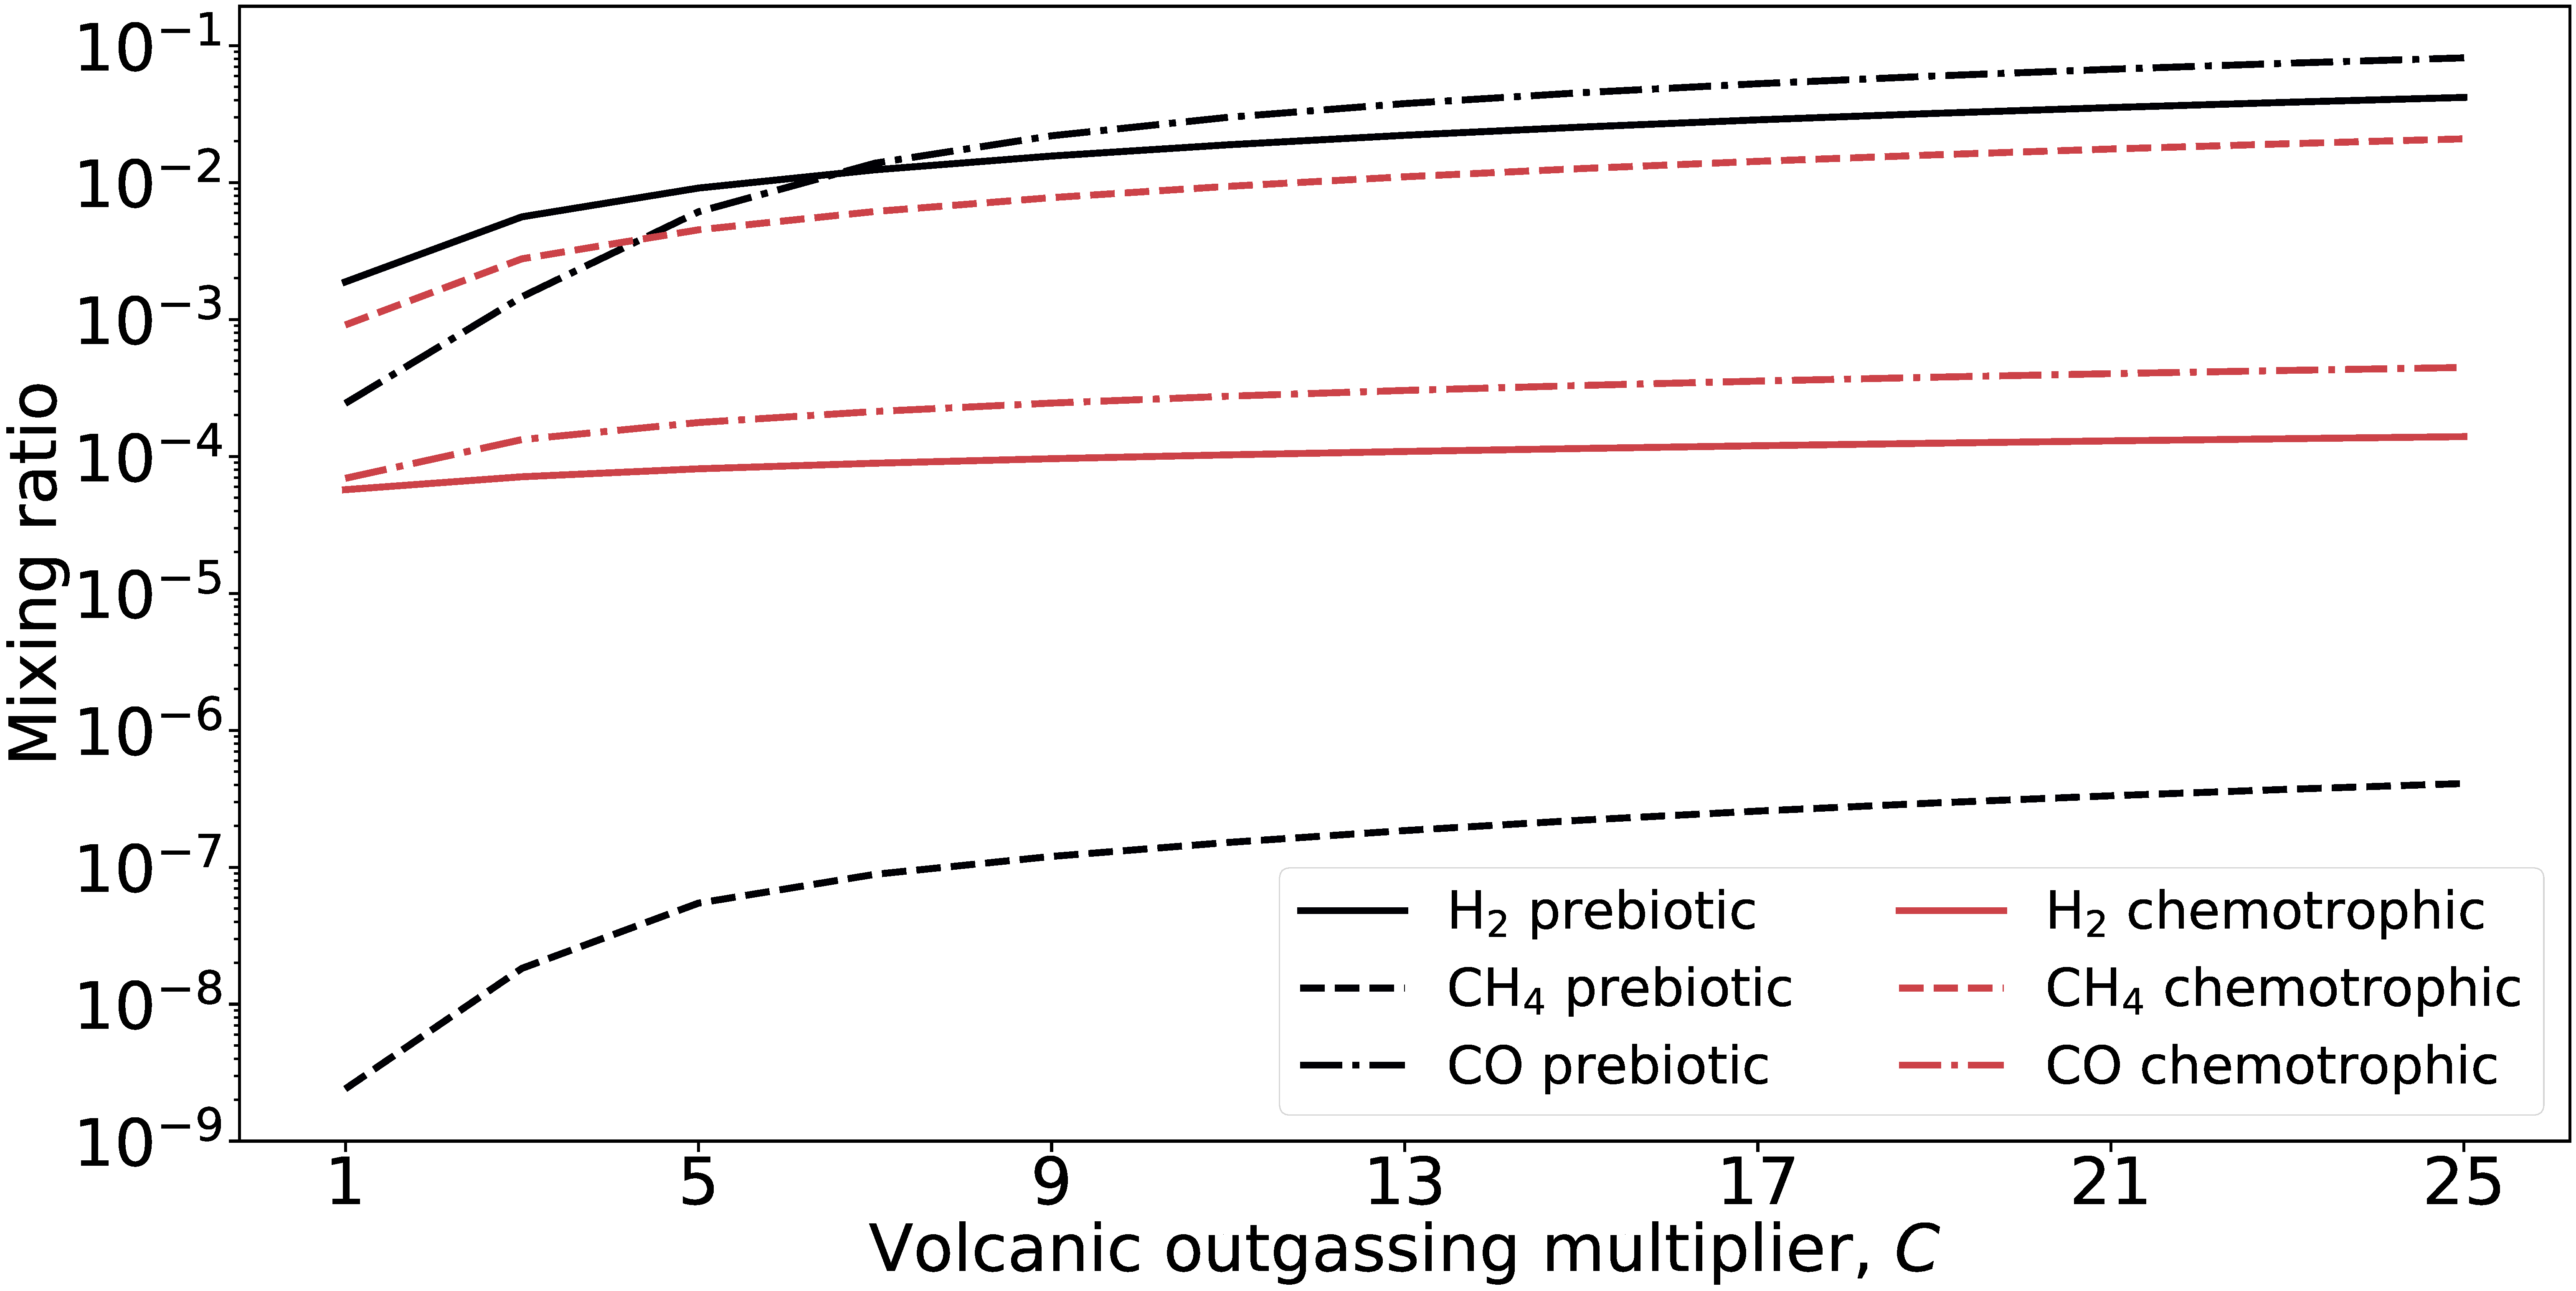
\includegraphics[width=0.9\textwidth]{tex/2diseq/Figure1.pdf}
  \caption{The mixing ratio of H$_2$, CH$_4$ and CO in the modeled prebiotic and chemotrophic early Earth atmospheres as a function of volcanic outgassing, relative to modern. Black lines represent mixing ratios for the prebiotic case. Red lines represent mixing ratios for the chemotrophic case where we have assumed an energy-limited ocean ecosystem. For both simulations, we also assume the mixing ratios of N$_2$ and CO$_2$ are 0.75 and 0.2 respectively. The presence of a chemotrophic biosphere drastically lowers H$_2$ abundances and increases CH$_4$ abundances due to methanogenesis, and lowers CO abundances because of acetogenesis.}
  \label{fig:diseq_figure1}
\end{figure}

Figure \ref{fig:diseq_figure2} shows the modeled atmosphere-ocean thermodynamic disequilibrium for the prebiotic and chemotrophic atmosphere as a function of the volcanic outgassing multiplier. For all outgassing scenarios, the chemotrophic atmosphere-ocean disequilibrium is lower than the prebiotic atmosphere-ocean disequilibrium because the biosphere exploits free energy for metabolism. Additionally, the atmosphere-only disequilibrium is always lower in the chemotrophic ecosystem than in the prebiotic ecosystem for the same reason.

\begin{figure}
  \centering
  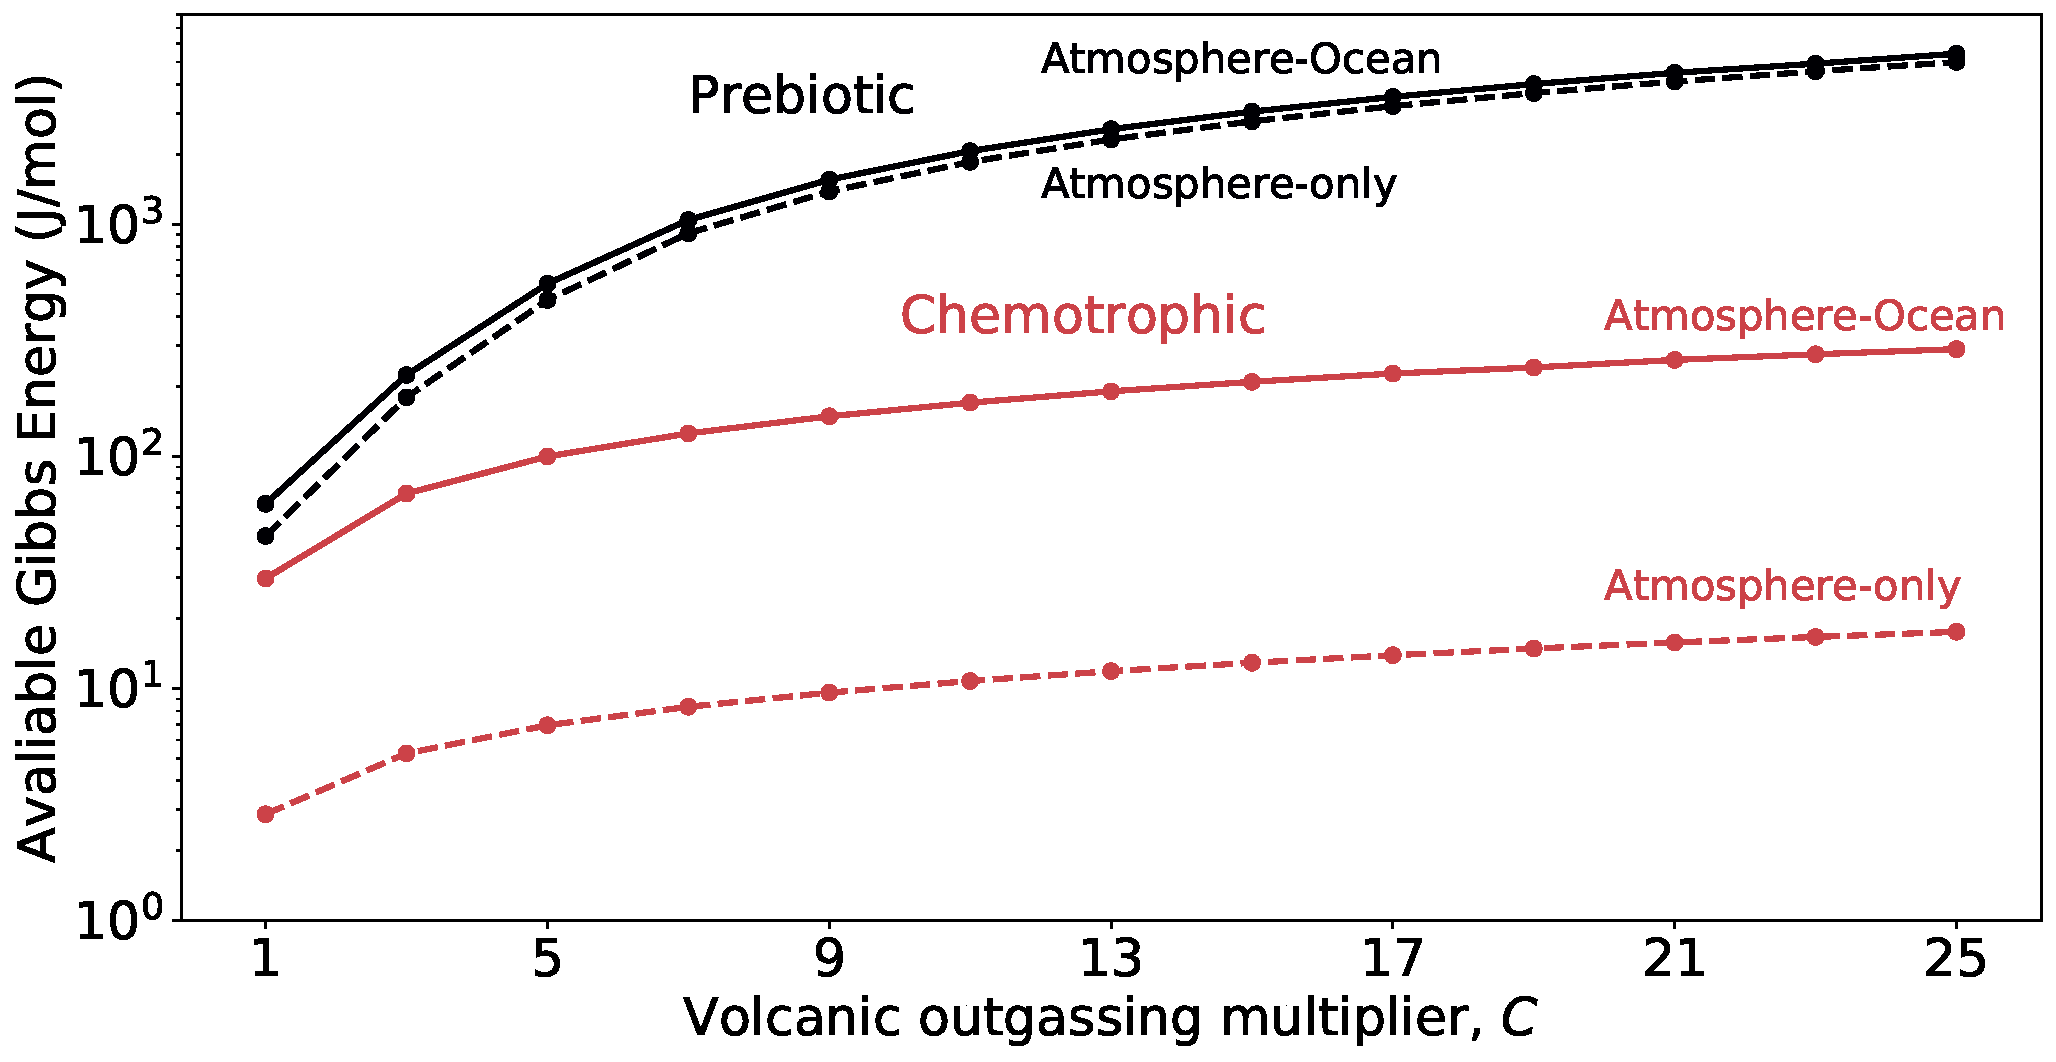
\includegraphics[width=0.9\textwidth]{tex/2diseq/Figure2.pdf}
  \caption{Chemical disequilibrium, as measured by available Gibbs energy, of the prebiotic (black lines) and chemotrophic (red lines) Earth as a function of a volcanic outgassing multiplier, relative to modern. The dotted lines are atmosphere-only Gibbs energy calculations, and the solid lines are atmosphere-ocean calculations. The presence of a chemotrophic ecosystem lowers both the atmosphere-ocean and atmosphere-only chemical disequilibrium by using the free energy for metabolism.}
  \label{fig:diseq_figure2}
\end{figure}

The following sections explain which species contribute most to the available Gibbs energy in both the prebiotic and chemotrophic model.

\subsection{The prebiotic disequilibrium and the species that contribute to it}

The available Gibbs energy of the prebiotic atmosphere-ocean system for modern volcanic outgassing rates ($C = 1$) is 62 J/mol of atmosphere (compared to 2326 J/mol for the modern biotic Earth \citep{KrissansenTotton_2016}). The largest source of disequilibrium is due to the coexistence of CO$_2$ and H$_2$ which accounts for $\sim 40$ J/mol (65\%) of this total available Gibbs energy. These molecules should react and form CH$_4$ and water vapor in equilibrium:

\begin{equation}
  4 \mathrm{H_2} + \mathrm{CO_2} \leftrightarrow \mathrm{CH_4} + 2 \mathrm{H_2O}
\end{equation}

The coexistence of CO and water vapor contributes $\sim 10$ J/mol (16\%), which is the second most important contributor to this available Gibbs energy. At equilibrium, H$_2$ and CO$_2$ will be replaced by CH$_4$ and CO$_2$ from the reaction

\begin{equation}
  4 \mathrm{CO} + 2 \mathrm{H_2O} \leftrightarrow 3 \mathrm{CO_2} + \mathrm{CH_4}
\end{equation}

Both the H$_2$-CO$_2$ and CO-H$_2$O disequilibrium ultimately come from volcanic outgassing. Gases were once in equilibrium with magma but have been emitted into a colder environment of the atmosphere where they are in disequilibrium. For higher outgassing scenarios, the H$_2$-CO$_2$ and CO-H$_2$O reactions remain the most import contributors to the available Gibbs energy. Since these reactions are in the gas phase, the atmosphere-only disequilibrium is nearly as large ($\sim 80\%$) as the atmosphere-ocean disequilibrium for all outgassing rates. For a possible Hadean outgassing rate of $C = 9$, $\Phi$ is 1555 J/mol.

\subsection{The chemotrophic disequilibrium and species that contribute to it}

The atmosphere-ocean available Gibbs energy of the chemotrophic Earth for modern volcanic outgassing rates ($C = 1$) is 30 J/mol. The coexistence of CO$_2$, CH$_4$, N$_2$, and liquid water contribute $\sim 24$ J/mol (80\%) to this available Gibbs energy. These four species should react and deplete 99.9\% of atmospheric methane in equilibrium

\begin{equation}
  \label{eq:chemo_diseq}
  5 \mathrm{CO_2} + 4 \mathrm{N_2} + 3 \mathrm{CH_4} + 14 \mathrm{H_2O} \leftrightarrow 8 \mathrm{NH_4^{+}} + 8 \mathrm{HCO_3^{-}}
\end{equation}
For volcanic outgassing 25 times modern fluxes ($C = 25$), this reaction accounts for $\sim 273$ J/mol (94\%) of the available Gibbs energy (290 J/mol), which shows that these species are the most important for all modeled chemotrophic systems. The atmosphere-only disequilibrium is always much smaller than the atmosphere-ocean disequilibrium because Equation \eqref{eq:chemo_diseq} involves disequilibrium with the liquid water ocean.

The H$_2$-CO$_2$ and CO-H$_2$O disequilibria, which dominate the prebiotic available Gibbs energy, contribute only $\sim 0.8$ J/mol and $\sim 2.4$ J/mol, respectively, for modern volcanic outgassing ($C = 1$). The minor contribution of these disequilibria persists for all volcanic outgassing scenarios.

\subsection{Disequilibrium though Earth history}

Figure \ref{fig:diseq_figure3} shows our estimates of the evolution of Earth's atmosphere-ocean and atmosphere-only disequilibrium through its history. The prebiotic and chemotrophic disequilibrium ranges are from this study (i.e., Figure \ref{fig:diseq_figure2}), and the estimates from the late Archean to the present are from \citet{KrissansenTotton_2018_diseq}. Figure \ref{fig:diseq_figure3} has a broken axis between the chemotrophic ecosystem and the Archean because the advent of anoxygenic photosynthesis would have likely influenced how disequilibrium changed between these two eras. Our modeling does not capture this transition for reasons discussed below.

\begin{figure}
  \centering
  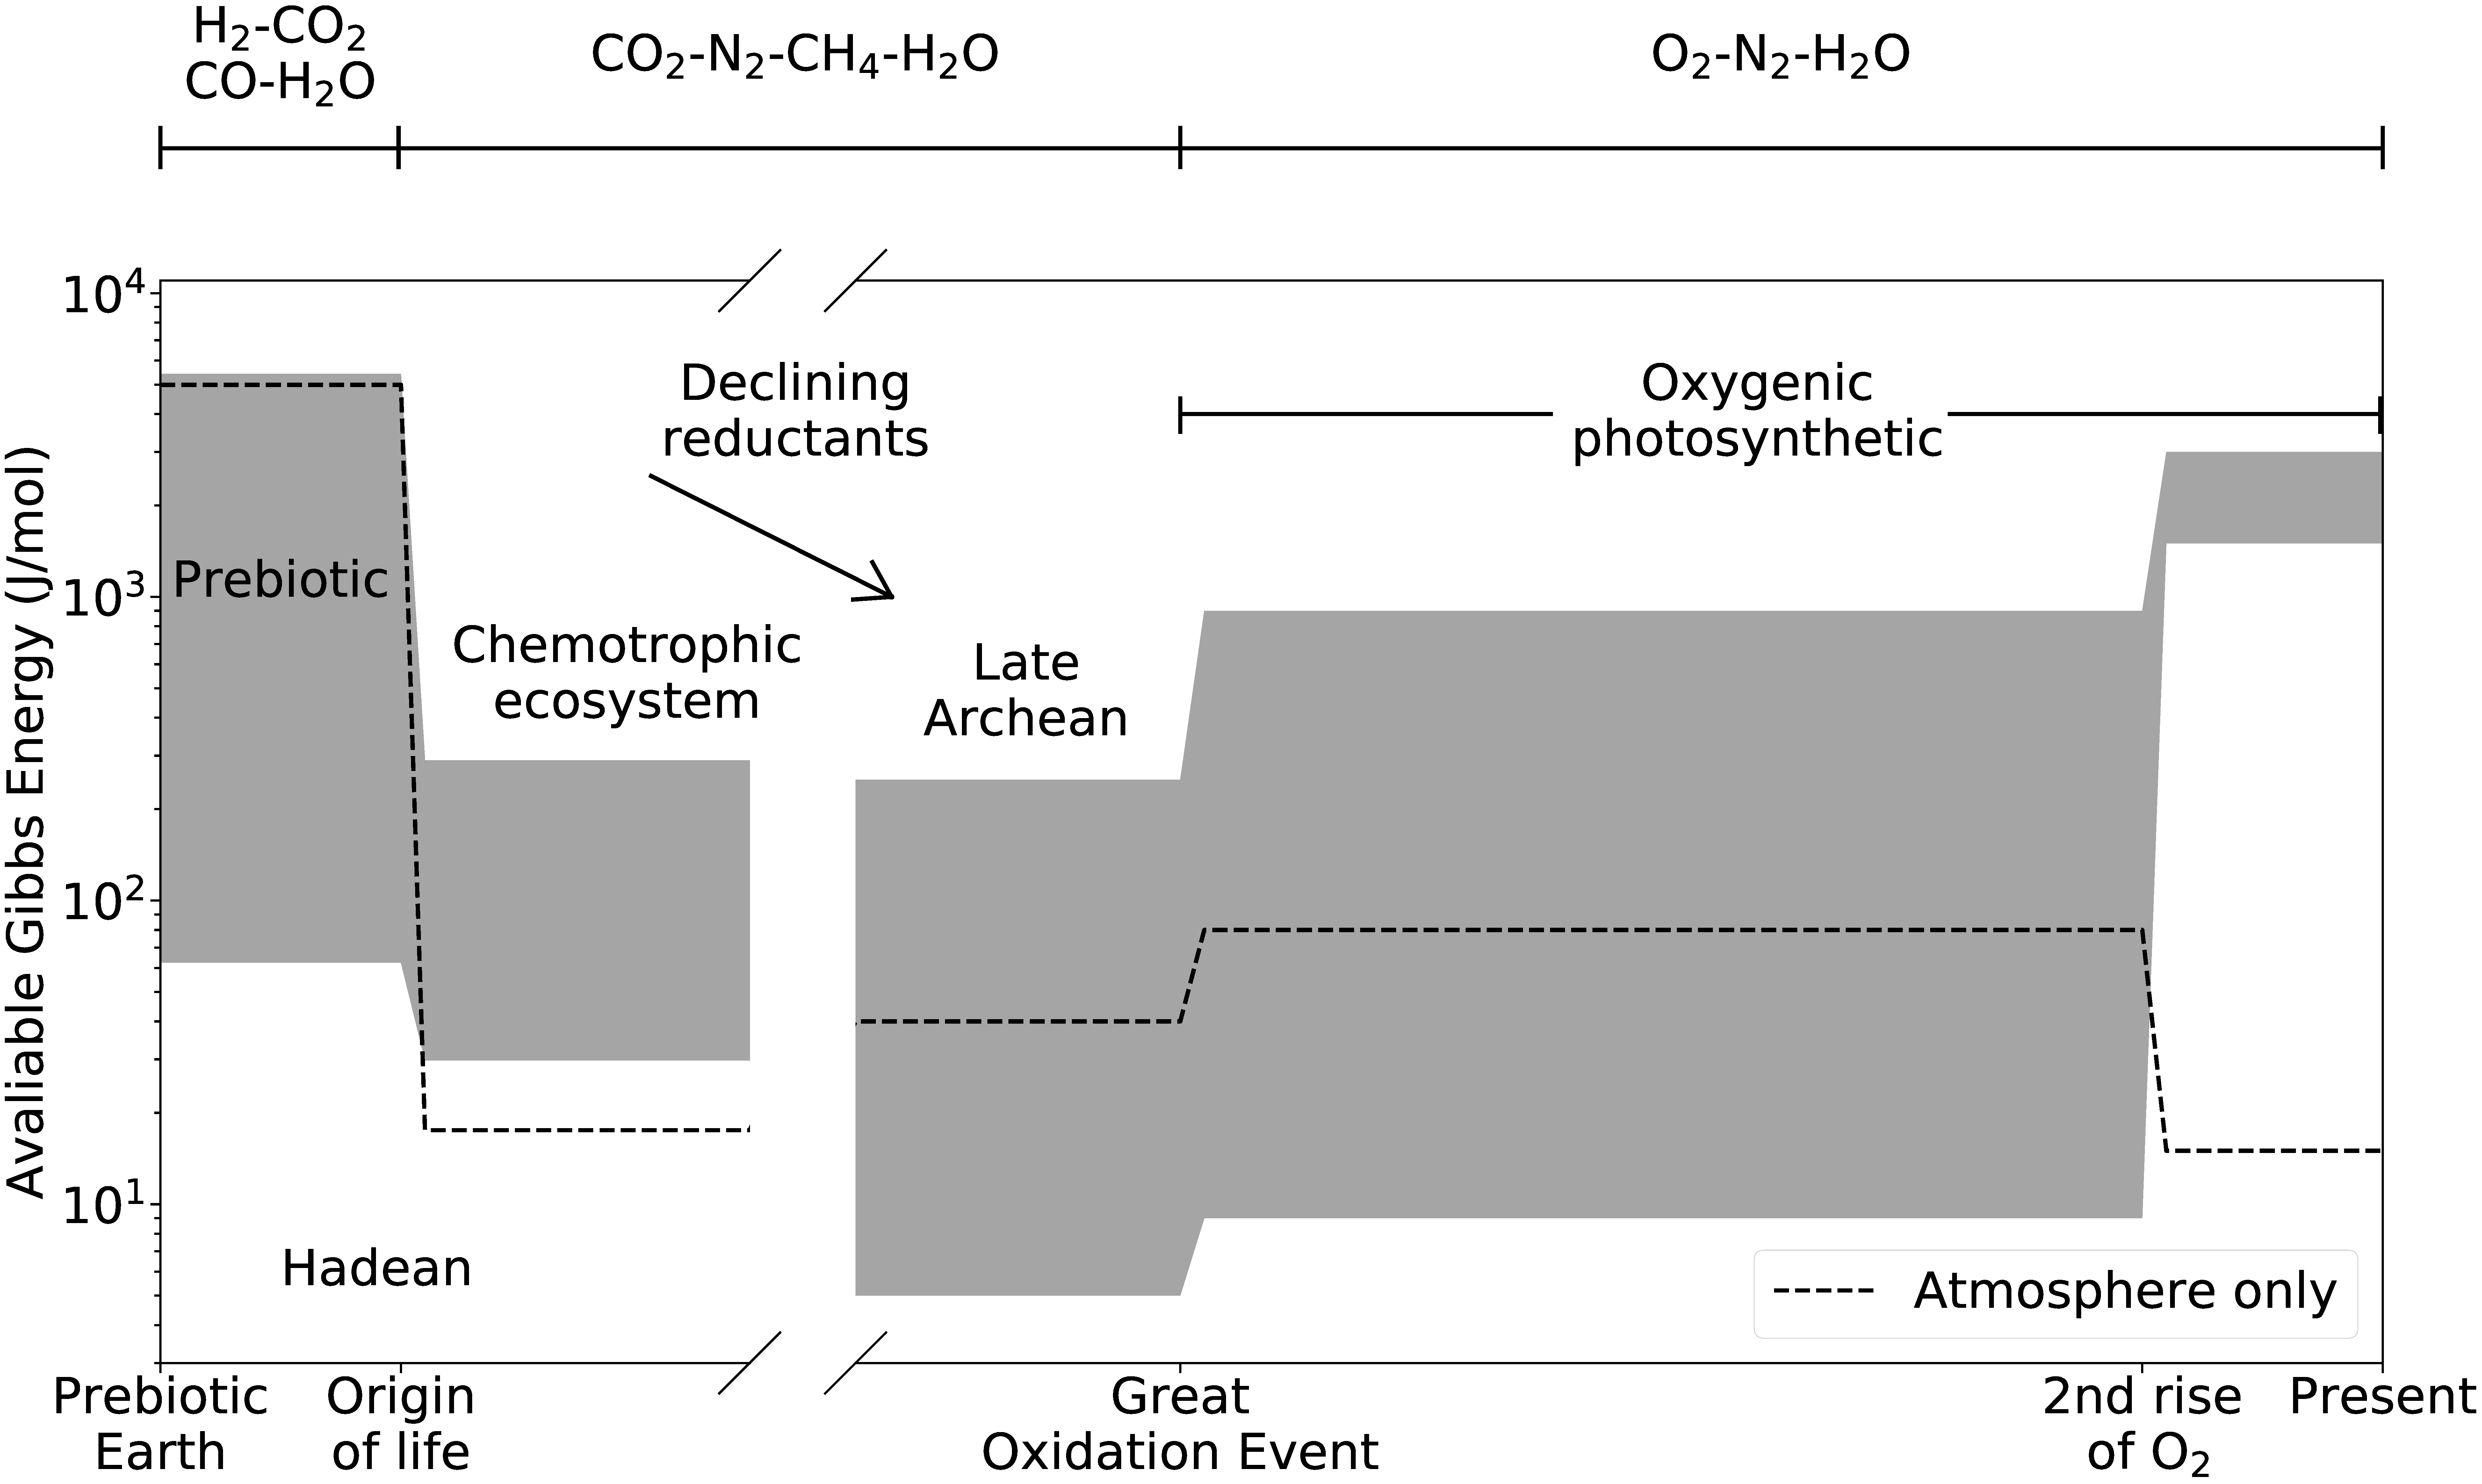
\includegraphics[width=1.0\textwidth]{tex/2diseq/Figure3.pdf}
  \caption{The chemical disequilibrium of Earth's atmosphere-ocean system through time. The shading indicates plausible ranges of atmosphere-ocean disequilibrium during intervals of Earth's history based on modeling (this study), and atmospheric proxies and models \citep{KrissansenTotton_2018_diseq}. The plot is broken between the ``chemotrophic ecosystem'' and ``Archean'' because the advent of anoxygenic photosynthesis would have likely influenced how disequilibrium changed between these two eras which is uncertain. The dotted line is the maximum atmosphere-only disequilibrium. Above the plot are the disequilibria (e.g., H$_2$-CO$_2$) that contribute most to the atmosphere-ocean available Gibbs energy. Throughout Earth's history, disequilibrium fell with the rise of chemotrophic life, and rose after of the oxygenation of Earth's atmosphere from oxygenic photosynthesis.}
  \label{fig:diseq_figure3}
\end{figure}

Like the chemotrophic Earth, the Archean disequilibrium was dominated by the coexistence of CO$_2$, CH$_4$, N$_2$, and liquid water \citep{KrissansenTotton_2018_diseq}. After the Great Oxidation Event, the magnitude of the available Gibbs energy rose, and was instead dominated by the coexistence O$_2$, N$_2$ and liquid water, which should react to form nitric acid at equilibrium:

\begin{equation}
  \label{eq:o2n2h2o_diseq_react}
  5 \mathrm{O_2} + 2 \mathrm{N_2} + 2 \mathrm{H_2O} \leftrightarrow 4 \mathrm{H^{+}} + 4 \mathrm{NO_3^{-}}
\end{equation}
The magnitude of the O$_2$-N$_2$-H$_2$O disequilibrium increased with the rise of O$_2$ until the present available Gibbs energy of 2326 J/mol \citep{KrissansenTotton_2016}. 

\section{Discussion}

\subsection{Life's impact on disequilibria through Earth's history}

Our results show that life has both generated and destroyed chemical disequilibrium in Earth's atmosphere-ocean system (Figure \ref{fig:diseq_figure3}). Pioneering work by \citet{Lovelock_1975}, which proposed using disequilibrium as a sign of life, argued that abiotic worlds would be close to thermodynamic equilibrium. However, this thinking ignored volcanically active planets. We showed that disequilibrium was likely high ($10^2$ to $10^3$ J/mol) in prebiotic times due to the volcanically produced H$_2$-CO$_2$ and CO-H$_2$O disequilibria.

Subsequently, if the first life was chemotrophic and metabolized H$_2$, CO$_2$, and CO, then the atmosphere-ocean disequilibrium would have dropped to $\sim 10^2$ J/mol with the rise of microbial life. This is an example of chemotrophic life destroying the disequilibrium of its environment and promoting chemical equilibrium on a global scale.

The invention of anoxygenic photosynthesis, which we did not consider, may have added to the Atmosphere-ocean disequilibrium in the late Archean. Iron oxidizing photosynthesis is an example: 

\begin{equation}
  4 \mathrm{Fe^{2+}} + \mathrm{CO_2} + 11 \mathrm{H_2O} + h\nu \rightarrow 4 \mathrm{Fe(OH)_3} + \mathrm{CH_2O} + 8 \mathrm{H^{+}}
\end{equation}

The CH$_2$O produced could have been processed by heterotrophs and methanogens yielding CH$_4$, which would have added to the Archean CO$_2$-N$_2$-CH$_4$-H$_2$O disequilibrium without the need for additional volcanic outgassing \citep{KrissansenTotton_2018_diseq}. Additionally, the CH$_2$O would also degrade into CO in the ocean, which would have added a small amount to the CO-H$_2$O disequilibrium \citep{Schwieterman_2019}. Figure \ref{fig:diseq_figure3} does not explicitly capture these effects because the evolutionary history of anoxygenic photosynthesis is uncertain, but Archean disequilibrium estimates allow for such photosynthesis \citep{KrissansenTotton_2018_diseq}.

Even though the rise of anoxygenic photosynthesis would have added to the late Archean disequilibrium, overall disequilibrium may have dropped because a lower flux of reductants would have been available to the biosphere. Before the rise of oxygenic photosynthesis, which uses ubiquitous water and sunlight, the biosphere is hypothesized to have been probably limited by the available reductants such as H$_2$, Fe$^{2+}$, and CO \citep{Canfield_2006}. For example, H$_2$-using anoxygenic phototrophs ($\mathrm{CO_2} + 2 \mathrm{H_2} + h\nu \rightarrow \mathrm{CH_2O} + \mathrm{H_2O}$) were likely limited by volcanically outgassed H$_2$. Volcanic outgassing of reductants probably declined from the Hadean to the late Archean as the Earth's interior cooled. Fewer available reductants would have lowered biological CH$_4$ production, resulting in smaller disequilibrium in the late Archean.

The increase of the available Gibbs energy and the rise of the O$_2$-N$_2$-H$_2$O disequilibrium after the Great Oxidation Event was primarily caused by oxygenic photosynthesis. Atmospheric O$_2$ comes directly from oxygenic photosynthesis, and N$_2$ is generated, in part, from denitrifying bacteria that are ultimately powered by organic material from photosynthesis. Disequilibrium increased again to near modern levels with a rise of O$_2$ to near modern levels through the Neoproterozoic and Paleozoic \citep{Krause_2018}.

\subsection{Why disequilibrium persists in Earth's atmosphere-ocean system despite the presence of biology}

Chemotrophs consumed a large fraction of Earth's prebiotic disequilibrium (Figure \ref{fig:diseq_figure2}), but microbes left the CO$_2$-N$_2$-CH$_4$-H$_2$O and O$_2$-N$_2$-H$_2$O disequilibrium uneaten in the Archean and Proterozoic eons and in modern times. Thus, a pertinent question is: Why didn't microbes evolve metabolisms to consume the ``free lunch'' that has persisted in Earth's atmosphere?

We propose that this lack of consumption is due to the kinetic barriers of the CO$_2$-N$_2$-CH$_4$-H$_2$O and O$_2$-N$_2$-H$_2$O reactions, which we hypothesize are insurmountable by enzymes. To illustrate this idea, consider the disequilibrium of O$_2$-N$_2$-H$_2$O. These species would react slowly in the atmosphere in the absence of life via a number of steps:

\begin{equation}
\begin{aligned}
  \mathrm{N_2} + 2 \mathrm{O} &\rightarrow 2 \mathrm{NO} + 2 \mathrm{N} \\
  2 \mathrm{N} + 2 \mathrm{O_2} &\rightarrow 2 \mathrm{NO} + 2 \mathrm{O} \\
  4 \mathrm{NO} + 2 \mathrm{O_2} &\rightarrow 4 \mathrm{NO_2} \\
  4 \mathrm{NO_2} + \mathrm{O_2} + 2 \mathrm{H_2O} &\rightarrow 4 \mathrm{HNO_3} \\
  4 \mathrm{HNO_3} &\rightarrow 4 \mathrm{H^{+}} + 4 \mathrm{NO_3^{-}}
\end{aligned}
\end{equation}

The first two reactions, which make NO, are Zeldovich's reactions \citep{Dixon_1984} and require lightning to heat the air to $\sim 20,000$ K \citep{Chameides_1977}. The third reaction occurs very quickly after the NO is generated \citep{Murray_2016}. The final two reactions are ultimately (partially) responsible for acid rain \citep{Platt_1986}. The rate limiting step to the net reaction is the first one, which has an activation energy of 316 kJ/mol \citep{Dixon_1984}. We take this to be a lower bound on the uncatalyzed activation energy of reacting O$_2$, N$_2$ and H$_2$O. This must be a lower bound because the rate limiting step requires the presence of atomic oxygen, which could only have come from splitting O$_2$ with additional energy.

Life harnesses the free energy of disequilibria by lowering activation energy barriers with enzymes. Figure \ref{fig:diseq_figure4}a is a classic textbook graph of free energy during an exothermic chemical reaction. Uncatalyzed reactions can only occur if a relatively large activation energy barrier is overcome. Therefore, many uncatalyzed reactions (between disequilibria) occur extremely slowly because ambient thermal energy is insufficient. Microbes tap into the free energy stored in disequilibria by using enzymes to lower activation energy barriers to levels where thermal energy allows reactions to proceed at appreciable rates. 

\begin{figure}
  \centering
  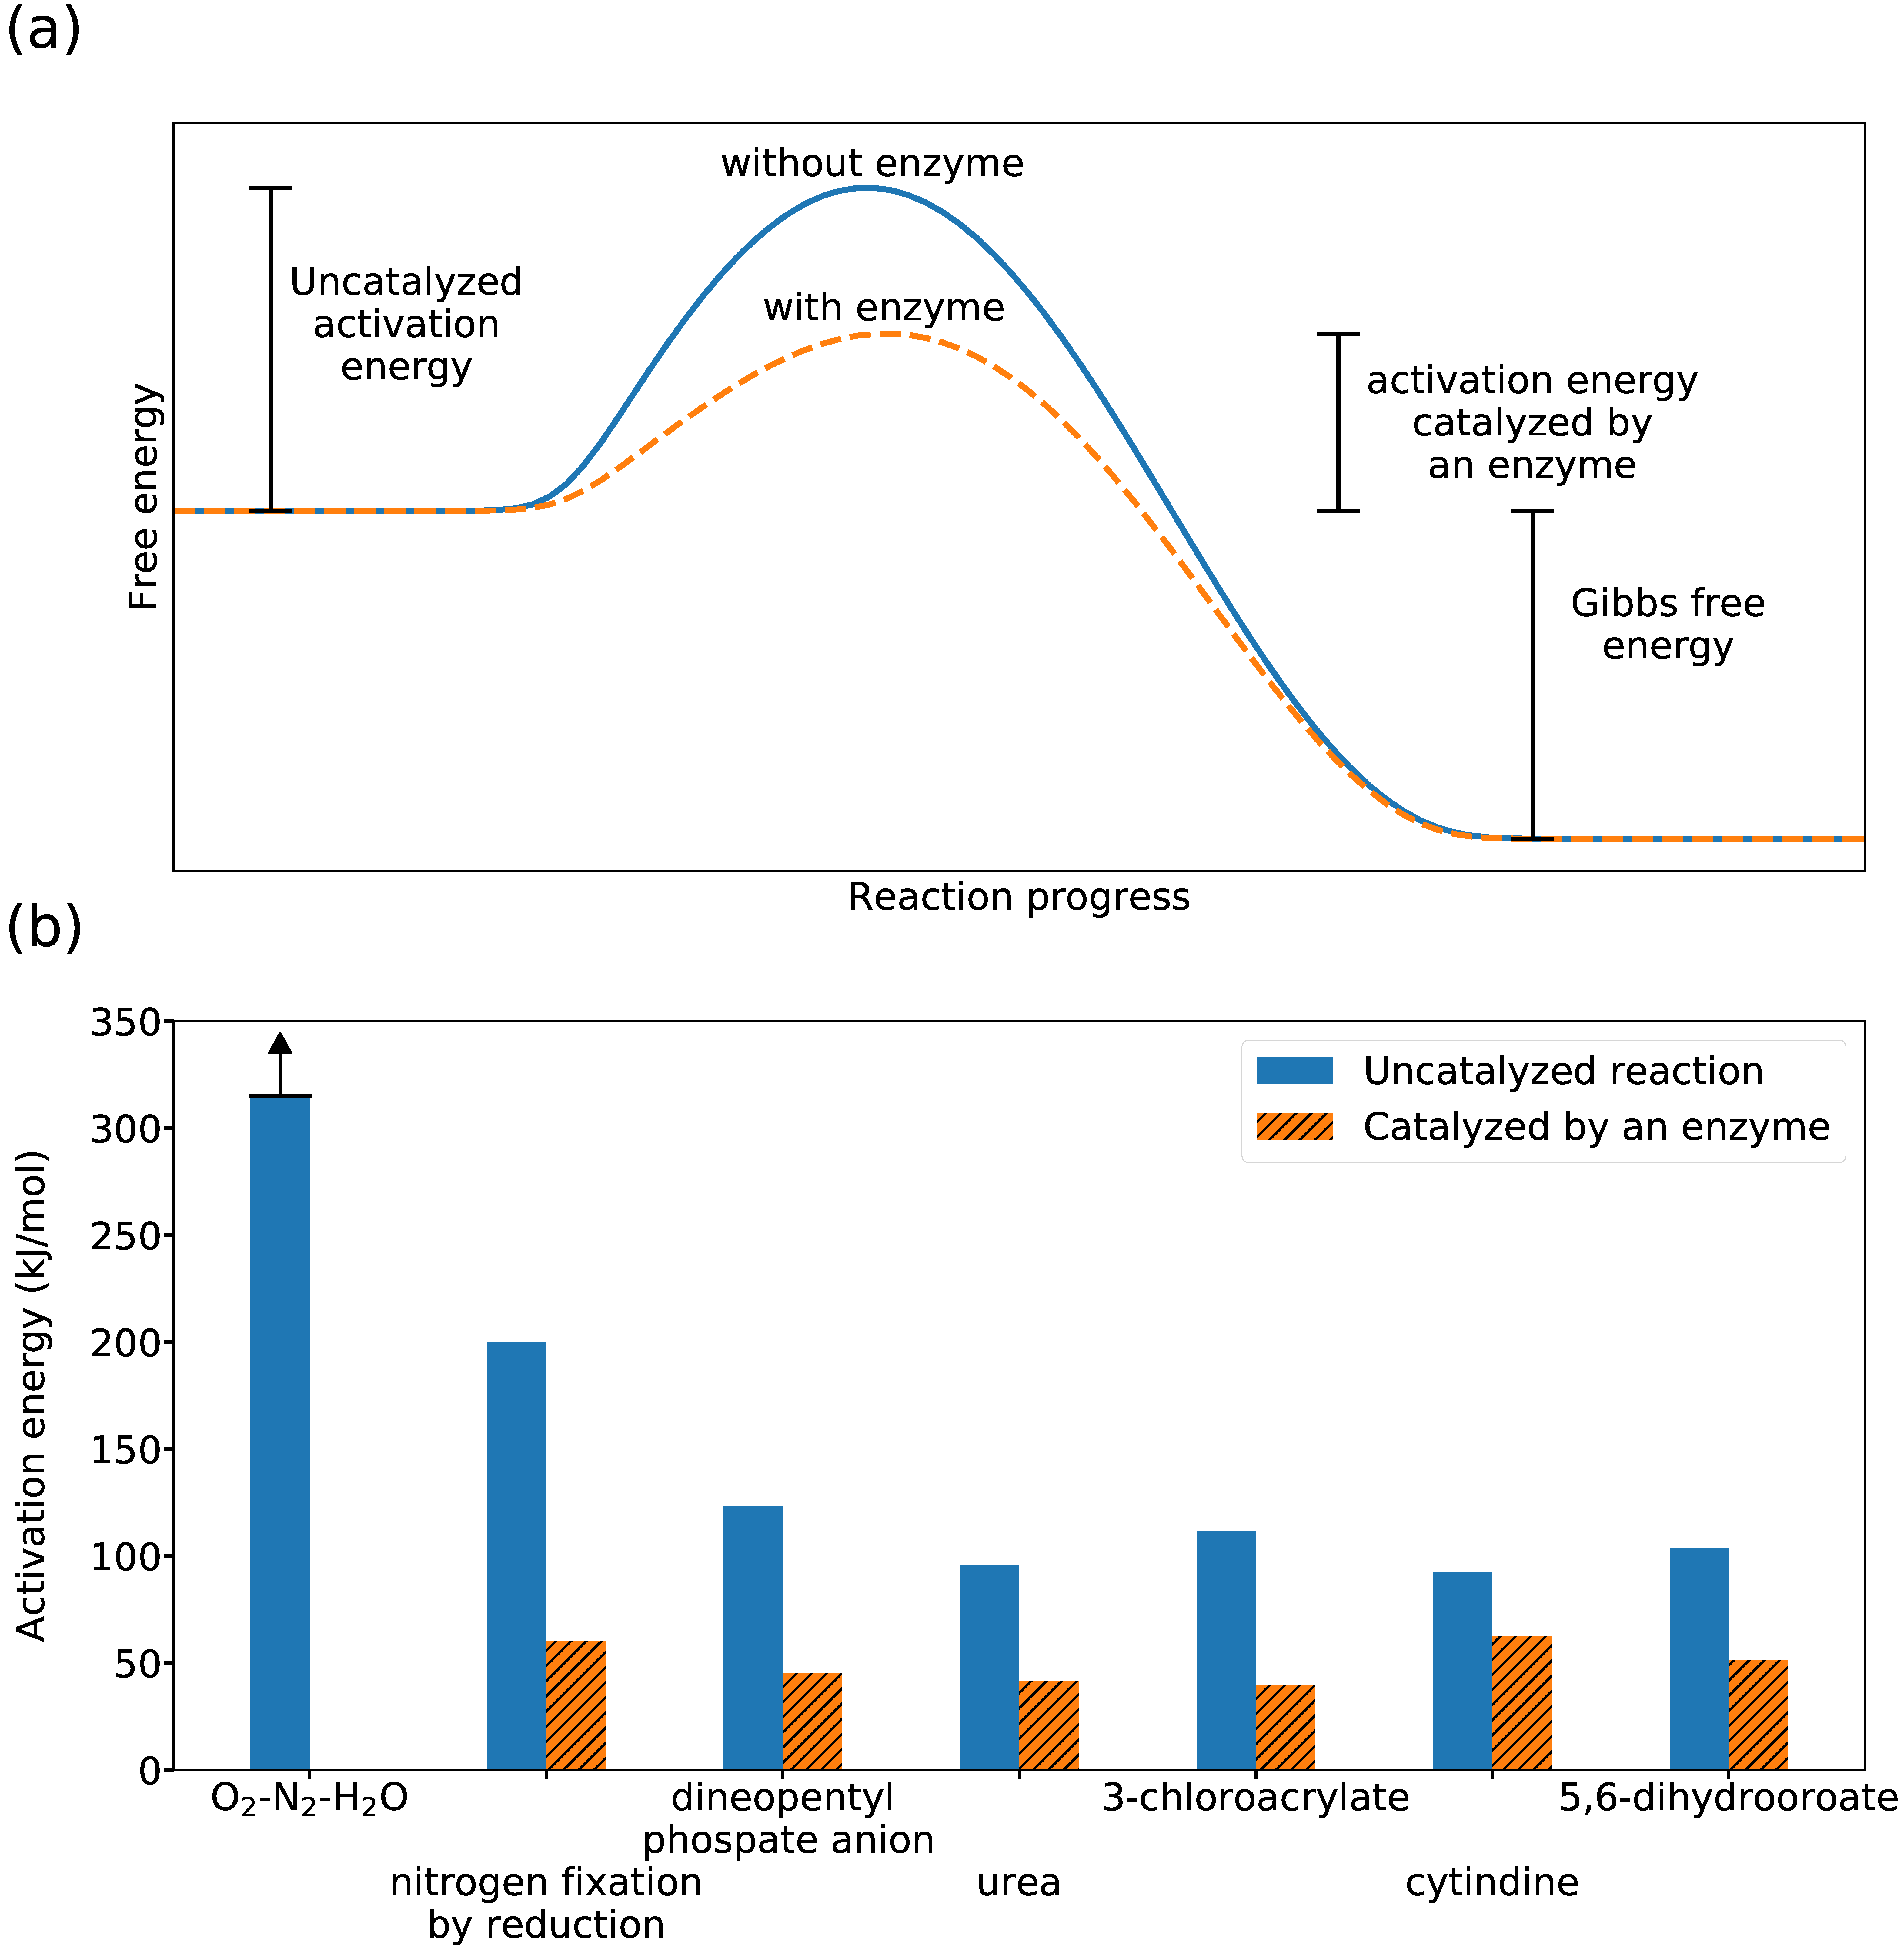
\includegraphics[width=1.0\textwidth]{tex/2diseq/Figure4.pdf}
  \caption{(a) Schematic of free energy during a chemical reaction. (b) The activation energy of several uncatalyzed reactions (blue), and reactions catalyzed by enzymes (orange). The lower bound for the uncatalyzed activation energy of O$_2$-N$_2$-H$_2$O (a reaction that life doesn't perform) is from \citet{Dixon_1984}, and the activation energy of nitrogen fixation is from a number of references \citep{Andersen_1977,Hageman_1980} (see 
  Appendix \ref{} % C
  for a summary of our literature search of nitrogen fixation kinetics). The rest of the activation energies are from 
  Table \ref{} % 4 
  in \citet{Wolfenden_2006}. The uncatalyzed activation energy of O$_2$-N$_2$-H$_2$O is notably larger than the uncatalyzed activation energy of reactions that life manages to perform, which we hypothesize explains why no life has evolved that can exploit the O$_2$-N$_2$-H$_2$O disequilibrium.}
  \label{fig:diseq_figure4}
\end{figure}

Figure \ref{fig:diseq_figure4}b compares the uncatalyzed activation energy of O$_2$-N$_2$-H$_2$O to the uncatalyzed activation energy (blue bars) of reactions that enzymes lower to $\sim 30$ to 60 kJ/mol, which allow reactions to proceed at normal temperatures. The reaction between O$_2$, N$_2$, and H$_2$O, which is not performed by life, has an activation energy that is higher than all other uncatalyzed reactions. This suggests that Reaction \eqref{eq:o2n2h2o_diseq_react} is not amenable to biological catalysis. The activation energy of O$_2$-N$_2$-H$_2$O is probably high because it involves breaking the triple bond in $\mathrm{N \equiv N}$ by oxidation. The reaction between CO$_2$, N$_2$, CH$_4$, and H$_2$O (Equation \eqref{eq:chemo_diseq}) also involves breaking an N$_2$ bond, so it potentially has an activation energy comparable to Reaction \eqref{eq:o2n2h2o_diseq_react} ($> 300$ kJ/mol).

Nitrogen fixing bacteria are the only organisms that break $\mathrm{N \equiv N}$ bonds by chemical reduction with the aid of the nitrogenase enzyme. The literature suggests that the uncatalyzed activation energy of nitrogen fixation by reduction is $\sim 200$ kJ/mol \citep{Hageman_1980}, which is $< 63\%$ of the uncatalyzed activation energy of Reaction \eqref{eq:o2n2h2o_diseq_react}. These differing energy barriers might explain why biology has managed to catalyze nitrogen fixation by reduction of N$_2$ but not by direct oxidation of N$_2$.

In summary, we speculate that life has not evolved to consume the CO$_2$-N$_2$-CH$_4$-H$_2$O and O$_2$-N$_2$-H$_2$O disequilibrium because these reactions are kinetically insurmountable for biology. We hypothesize that these reactions will be biochemically prohibited elsewhere on Earth-like exoplanets, which is a testable hypothesis 
(Section \ref{}).

\subsection{Chemical disequilibrium as a biosignature or anti-biosignature}


% Chapter 3
\chapter{The Likelihood of CH\textsubscript{4}+CO\textsubscript{2} Biosignature False Positives from Volcanism}
\newpage

\noindent \textit{This chapter was originally published in collaboration with Joshua Krissansen-Totton and David C. Catling in the Planetary Science Journal \citep{Wogan_2020_methane}, and is reproduced below with the permission of the journal.}

\section*{\centering Summary}

The disequilibrium combination of abundant methane and carbon dioxide has been proposed as a promising exoplanet biosignature that is readily detectable with upcoming telescopes such as the James Webb Space Telescope. However, few studies have explored the possibility of non-biological CH$_4$ and CO$_2$ and related contextual clues. Here, we investigate whether magmatic volcanic outgassing on terrestrial planets can produce atmospheric CH$_4$ and CO$_2$ with a thermodynamic model. Our model suggests that volcanoes are unlikely to produce CH$_4$ fluxes comparable to biological fluxes. Improbable cases where volcanoes produce biological amounts of CH$_4$ also produce ample carbon monoxide. We show, using a photochemical model, that high abiotic CH$_4$ abundances produced by volcanoes would be accompanied by high CO abundances, which could be a detectable false positive diagnostic. Overall, when considering known mechanisms for generating abiotic CH$_4$ on terrestrial planets, we conclude that observations of atmospheric CH$_4$ with CO$_2$ are difficult to explain without the presence of biology when the CH$_4$ abundance implies a surface flux comparable to modern Earth's biological CH$_4$ flux. A small or negligible CO abundance strengthens the CH$_4$+CO$_2$ biosignature because life readily consumes atmospheric CO, while reducing volcanic gases likely cause CO to build up in a planet's atmosphere. Furthermore, the difficulty of volcanically-generated CH$_4$-rich atmospheres suitable for an origin of life may favor alternatives such as impact-induced reducing atmospheres.

\section{Introduction} \label{sec:intro}

Large telescopes will soon be used to search for biogenic waste gases in exoplanet atmospheres. Oxygen is the most extensively studied biosignature gas \citep{Meadows_2017,Meadows_2018}. Although many studies have proposed ways of identifying scenarios where non-living processes might mimic life by producing oxygen, i.e. false positives \citep{Domagal-Goldman_2014,Harman_2015,Luger_2015,Schwieterman_2019,Tian_2014,Wordsworth_2014}, the circumstances are unusual and contextual clues can distinguish abiotic scenarios \citep{Meadows_2018}.

However, even when life is present, oxygen biosignatures may be uncommon. Oxygenic photosynthesis is a complex metabolism that only evolved once on Earth \citep{Fischer_2016}. Additionally, oxygen was slow to accumulate in the Earth's atmosphere \citep{Lyons_2014}, and other planets may have low O$_2$ concentrations for billions of years despite having oxygenic photosynthetic life if there are large oxygen sinks \citep{Claire_2006}. Accumulation of oxygen may be especially challenging on planets orbiting M-dwarf stars due to their low visible photon flux, which potentially limits primary production \citep{Lehmer_2018}.

One alternative to detecting oxygen-rich planets like the modern Earth is to look for methane on planets like the Archean Earth. Before the rise of oxygen, methanogenic life could have sustained a methane-rich atmosphere, which could be detected with remote spectroscopy \citep{Kasting_2003,Schindler_2000}. 

Recently, \citet{KrissansenTotton_2018_diseq} proposed a criterion for methane biosignatures: finding abundant CH$_4$ in the presence of CO$_2$ (abbreviated CH$_4$+CO$_2$). This combination is compelling if the CH$_4$ mixing ratio is greater than 0.1\% because it is difficult to explain such an abundance with the short atmospheric lifetime of CH$_4$ in terrestrial atmospheres and non-biological methane sources such as serpentinization \citep{KrissansenTotton_2018_diseq}. This 0.1\% threshold value is for planets that orbit stars like the Sun and must be adjusted for different stellar types. For example, planets orbiting M-stars typically receive less near-UV radiation than planets orbiting Sun-like stars resulting in different photochemistry that promotes the build up of CH$_4$ \citep{Segura_2005,Grenfell_2007,Grenfell_2014,Rugheimer_2015,Rugheimer_2018}. \citet{KrissansenTotton_2018_diseq} argued that the CH$_4$ biosignature is strengthened by a low CO abundance because volcanoes that produce CH$_4$ should also likely generate CO. Additionally, living planets might have low CO because microbes consume CO \citep{Kharecha_2005}; coupled ecosystem-planetary models of the early Earth suggest atmospheric CO/CH$_4$ ratios declined dramatically with the emergence of chemoautotrophic ecosystems \citep{Sauterey_2020}.

Exploring false positives for methane biosignatures is timely. Biogenic O$_2$ or O$_3$ detections with upcoming telescopes such as the James Webb Space Telescope (JWST) will be extremely difficult \citep{Barstow_2016,KrissansenTotton_2018_detect,Lustig-Yaeger_2019,Wunderlich_2020,Fauchez_2019}, whereas CH$_4$+CO$_2$ biosignatures are more readily detectable. Indeed, an Archean-Earth like CH$_4$+CO$_2$ biosignature is potentially detectable on the planet TRAPPIST-1e with just 10 transits \citep{KrissansenTotton_2018_detect}. Thus, exploration of potential methane biosignature false positives and their contextual discriminants is needed.

The literature exploring false positives for methane biosignatures has primarily focused on CH$_4$ generation in deep-sea serpentinizing hydrothermal vents. \citet{Guzman-Marmolejo_2013} estimated a maximum CH$_4$ surface flux of 0.18 Tmol/yr ($6.8\times10^8$ molecules cm$^{-2}$ s$^-1$) from hydrothermal vents for planets with the same mass as Earth. Additionally, \citet{KrissansenTotton_2018_diseq} used Monte-Carlo simulations to estimate a probability distribution for maximum abiotic CH$_4$ production from this process. They suggest that $>$10 Tmol CH4/yr is highly unlikely. These estimated maximum fluxes are small compared to modern Earth's biological CH$_4$ flux of 30 Tmol/yr. 

However, investigations of abiotic CH$_4$ on Earth suggest that these estimates of abiotic CH$_4$ from hydrothermal vents are potentially unrealistically large. Serpentinization reactions involving water and ultramafic oceanic crust generate H$_2$ then, purportedly, H$_2$ might react with inorganic carbon in hydrothermal systems to generate CH$_4$. \citet{KrissansenTotton_2018_diseq} and \citet{Guzman-Marmolejo_2013} both estimated abiotic CH$_4$ fluxes assuming efficient reactions between H$_2$ and inorganic carbon. However, laboratory experiments have shown that, uncatalyzed, this reaction is extremely slow at hydrothermal vent temperatures and pressures preventing chemical equilibrium on timescales of at least months \citep{Reeves_2020}. Additionally, various lines of evidence suggest that much of the CH$_4$ observed in deep-sea hydrothermal vent waters is ultimately from biology \citep{Reeves_2020}. Furthermore, lifeless planets without silica-secreting organisms should have high ocean-water SiO$_2$ concentrations which suppresses the H$_2$, and therefore abiotic CH$_4$, produced from serpentinization \citep{Tutolo_2020}.

Impacts can likely generate abiotic CH$_4$ \citep{Zahnle_2020}, although impact-generated CH$_4$ is only probable early in a solar system's lifetime. The cratering record on the Moon shows that Earth's impact flux decreased dramatically by 3.5 Ga \citep{Marchi_2014}. Thus, extra solar systems that are several billion years old are probably unlikely to have abiotic CH$_4$ from this source.

Here, we investigate another potential false-positive for the CH$_4$+CO$_2$ biosignature: magma-sourced volcanic outgassing (i.e., not metamorphic). Negligible CH$_4$ has been observed in gases emitted by magmatic volcanoes on Earth \citep{Reeves_2020,Catling_2017}, although it has not been investigated whether substantial CH$_4$ is feasible for volcanoes in vastly different thermodynamic regimes. We simulate outgassing speciation for a range of magma temperatures, outgassing pressures, oxygen fugacities, volatile composition, and variable partitioning between subaerial and submarine volcanism. We examine whether volcanoes can produce CH$_4$ fluxes comparable to biological fluxes. Using a photochemical model we also investigate atmospheric composition of hypothetical planets with reducing volcanic gases to see whether volcanic CH$_4$ coincides with large atmospheric CO, which could be a detectable false positive marker. 

\section{Methods} \label{sec:methods}

\subsection{Model for calculating volcanic outgassing speciation} \label{sec:volcmodel}

Below, we describe our model for predicting the gases produced by an erupting mantle-sourced volcano. We follow \citet{Gaillard_2014} and solve for the gas-gas and gas-melt equilibrium in a C-O-H system. Our model differs from \citet{Gaillard_2014} because we do not consider nitrogen or sulfur species. Despite these differences, we obtain similar results to calculations made in \citet{Gaillard_2014}. We have also validated our code against the work of \citet{Liggins_2020} and \citet{Ortenzi_2020}, which have independently constructed similar outgassing models. Our Python code is published as an open-source software on the Github page https://github.com/Nicholaswogan/VolcGases. 

Figure \ref{fig:imagine} shows a highly schematic conceptualization of volcanic degassing typical of low-viscosity magma. Gas bubbles form in the magma when molecules like H$_2$O and CO$_2$ are exsolved. Within the gas bubbles, reactions drive the system to chemical equilibrium. The oxygen fugacity ($f_{\mathrm{O_2}}$) of the gas bubble is controlled by equilibrium with the oxygen fugacity of the magma \citep[e.g.][]{Kadoya_2020}. Gases bubbles are released from the magma and enter the overlying atmosphere or ocean.

\begin{figure*}
    \centering
    \includegraphics[width=\textwidth]{tex/3methane/figures/whole_thing_pretty_filled_v2.pdf}
    \caption{Qualitative sketch of degassing typical of low viscosity magma (e.g., Hawaiian volcanoes). Here, gas bubble reaches thermal and chemical equilibrium with a melt (no crystals are present). Note, degassing can occur in many different ways depending on magma viscosity and volatile content \citep{Gonnermann_2013}.}
    \label{fig:imagine}
\end{figure*}

\renewcommand{\arraystretch}{1.1}
\begin{table}
\caption{Model constants and variables}
\label{tab:1}
\centering
\begin{tabularx}{\textwidth}{l c c c >{\raggedright\arraybackslash}p{4.5cm}}
\hline \hline
&Constant or Variable & Value & Units & Definition   \\
\hline
\multirow{11}{*}{Constants}& $d_\mathrm{H_2O}$     & 2.3   & ...     & Solubility constant$^a$ \\
&$a_\mathrm{CO_2}$     & 1     & ...     & Solubility constant$^a$ \\
&$a_\mathrm{H_2O}$     & 0.54  & ...     & Solubility constant$^a$ \\
&$S_1$     & ... & ...     & Solubility constant$^a$ \\
&$S_2$     & ... & ...     & Solubility constant$^a$ \\
&$\mu_\mathrm{magma}$     & 64.52 & $\frac{\text{g magma}}{\text{mol magma}}$ & Molar mass of magma$^b$ \\
&$\mu_\mathrm{H_2O}$     & 18.02 & $\frac{\mathrm{g\:H_2O}}{\mathrm{mol\:H_2O}}$ & Molar mass of H$_2$O \\
&$\mu_\mathrm{CO_2}$     & 44.01 & $\frac{\mathrm{g\:CO_2}}{\mathrm{mol\:CO_2}}$ & Molar mass of CO$_2$ \\
&$K_1$     & $e^{-29755/T+6.55}$ & bar$^{0.5}$ & Equilibrium constant$^c$ \\
&$K_2$     & $e^{-33979/T+10.42}$     & bar$^{0.5}$ & Equilibrium constant$^c$ \\
&$K_3$     & $e^{-96444/T+0.22}$     & -     & Equilibrium constant$^c$ \\

\hline
\multirow{5}{*}{Input} &$P$&...& bar   & Total pressure of degassing \\
      &$T$      &...& K     & Temperature of magma and gas \\
      &$f_{\mathrm{O_2}}$      &...& bar   & Oxygen fugacity of the magma \\
      &$m_{\mathrm{CO_2}}^{\mathrm{tot}}$       &...& $\frac{\mathrm{g\:CO_2}}{\mathrm{g\:gas\:and\:magma}}$ & mass fraction CO$_2$ in magma before degassing \\
      &$m_{\mathrm{H_2O}}^{\mathrm{tot}}$       &...& $\frac{\mathrm{g\:H_2O}}{\mathrm{g\:gas\:and\:magma}}$ & mass fraction H$_2$O in magma before degassing \\\hline
\multirow{8}{*}{Output} & $x_{\mathrm{H_2O}}$      &...& $\frac{\mathrm{mol\:H_2O}}{\mathrm{mol\:magma}}$ & mol fraction of H$_2$O in the magma after degassing \\
      &$x_{\mathrm{CO_2}}$       &...& $\frac{\mathrm{mol\:CO_2}}{\mathrm{mol\:magma}}$ & mol fraction of CO$_2$ in the magma after degassing \\
      &$P_{\mathrm{H_2O}}$       &...& bar   & Partial pressure of H$_2$O \\
      &$P_{\mathrm{CO_2}}$       &...& bar   & Partial pressure of CO$_2$ \\
      &$P_{\mathrm{H_2}}$       &...& bar   & Partial pressure of H$_2$ \\
      &$P_{\mathrm{CO}}$       &...& bar   & Partial pressure of CO \\
      &$P_{\mathrm{CH_4}}$       &...& bar   & Partial pressure of CH$_4$ \\
      &$\alpha_{\mathrm{gas}}$       &...& $\frac{\mathrm{mol\:gas}}{\mathrm{mol\:gas\:and\:magma}}$ & mol fraction in gas phase \\
\hline
\multicolumn{5}{>{\raggedright\arraybackslash}p{\textwidth}}{
$^a$From \citet{Iacono-Marziano_2012}. See Chapter Appendix \ref{sec:solu_constants} to calculate $S_1$ and $S_2$.

$^b$Molar mass of Mt. Etna magma.

$^c$Calculated from the NASA thermodynamic database \citep{Burcat_2005}.}
\end{tabularx}
\end{table}

A mathematical model describes the volatiles in gas bubbles and magma. The amount of carbon and hydrogen that are exsolved by the magma into bubbles is governed by the solubility of CO$_2$ and H$_2$O, which we calculate with the solubility relations for mafic magmas described in \citet{Iacono-Marziano_2012}:
\begin{equation}\label{eq:solu1}
    \ln ({x_{{\text{C}}{{\text{O}}_{\text{2}}}}}) = {x_{{{\text{H}}_{\text{2}}}{\text{O}}}}{d_{{{\text{H}}_{\text{2}}}{\text{O}}}} + {a_{{\text{C}}{{\text{O}}_{\text{2}}}}}\ln ({P_{{\text{C}}{{\text{O}}_{\text{2}}}}}) + S_1
\end{equation}
\begin{equation}\label{eq:solu2}
    \ln ({x_{{{\text{H}}_{\text{2}}}{\text{O}}}}) = {a_{{{\text{H}}_{\text{2}}}{\text{O}}}}\ln ({P_{{{\text{H}}_{\text{2}}}{\text{O}}}}) + {S_1}
\end{equation}
Here, $x_\mathrm{CO_2}$ and $x_\mathrm{H_2O}$ are mol fractions of CO$_2$ and H$_2$O in the magma, respectfully. Additionally, $P_\mathrm{CO_2}$ and $P_\mathrm{H_2O}$ are the partial pressure of CO$_2$ and H$_2$O in gas bubbles suspended in the magma. The other terms in Equations \eqref{eq:solu1} and \eqref{eq:solu2} are solubility parameters with values shown in Table \ref{tab:1} except $S_1$ and $S_2$, which are further described in Chapter Appendix \ref{sec:solu_constants}. We use solubility relations appropriate for mafic magmas because rocky planets and moons in our solar system usually have basaltic crusts which suggests that mafic magma is common to most terrestrial bodies.

Volatile mol fractions (e.g., $x_\mathrm{H_2O}$) can be converted to mass fractions with the formula
\begin{equation} \label{eq:convert}
    {m_i} = \frac{{x_i}{\mu_i}}{\mu_\mathrm{magma}}
\end{equation}
Here, $m_i$ is mass fraction, $\mu_i$ is the volatile's molar mass, and $i$ can be either H$_2$O or CO$_2$. Table \ref{tab:1} gives the units of each term. 

We assume that after the hot gas exsolves from the magma into bubbles, it achieves thermodynamic equilibrium from the reactions
\begin{equation}
    {{\text{H}}_{\text{2}}}{\text{O}} \leftrightarrow {{\text{H}}_{\text{2}}}{\text{ + }}\frac{{\text{1}}}{{\text{2}}}{{\text{O}}_{\text{2}}}
\end{equation}
\begin{equation}
    {\text{C}}{{\text{O}}_{\text{2}}} \leftrightarrow {\text{CO + }}\frac{{\text{1}}}{{\text{2}}}{{\text{O}}_{\text{2}}}
\end{equation}
\begin{equation}
    {\text{C}}{{\text{O}}_{\text{2}}}{\text{ + 2}}{{\text{H}}_{\text{2}}}{\text{O}} \leftrightarrow {\text{C}}{{\text{H}}_{\text{4}}}{\text{ + 2}}{{\text{O}}_{\text{2}}}
\end{equation}
At thermodynamic equilibrium, the ratios of the fugacities of volatile species (denoted $f_i$) are related to the equilibrium constant corresponding to each chemical reaction. We assume that we can replace fugacities with partial pressures (denoted $P_i$). This approximation is reasonable for the temperatures and pressures involved in volcanic outgassing \citep{Holland_1984}. Thus,
\begin{equation}\label{eq:react1}
    {K_1} = \frac{{{f_{{{\text{H}}_2}}}f_{{{\text{O}}_{\text{2}}}}^{0.5}}}{{{f_{{{\text{H}}_{\text{2}}}{\text{O}}}}}} \approx \frac{{{P_{{{\text{H}}_2}}}f_{{{\text{O}}_{\text{2}}}}^{0.5}}}{{{P_{{{\text{H}}_{\text{2}}}{\text{O}}}}}}
\end{equation}
\begin{equation}\label{eq:react2}
    {K_2} = \frac{{{f_{{\text{CO}}}}f_{{{\text{O}}_2}}^{0.5}}}{{{f_{{\text{C}}{{\text{O}}_2}}}}} \approx \frac{{{P_{{\text{CO}}}}f_{{{\text{O}}_2}}^{0.5}}}{{{P_{{\text{C}}{{\text{O}}_2}}}}}
\end{equation}
\begin{equation}\label{eq:react3}
    {K_3} = \frac{{{f_{{\text{C}}{{\text{H}}_4}}}f_{{{\text{O}}_2}}^2}}{{{f_{{\text{C}}{{\text{O}}_2}}}f_{{{\text{H}}_2}{\text{O}}}^2}} \approx \frac{{{P_{{\text{C}}{{\text{H}}_4}}}f_{{{\text{O}}_2}}^2}}{{{P_{{\text{C}}{{\text{O}}_2}}}P_{{{\text{H}}_2}{\text{O}}}^2}} 
\end{equation}
We calculate equilibrium constants (e.g. $K_1$) using the NASA thermodynamic database \citep{Burcat_2005}. We assume that the gas is thermally and chemically coupled to the magma so that the oxygen fugacity ($f_\mathrm{O_2}$) of the gas is set by the oxygen fugacity of magma, as observed \citep{Symonds_1994}.  So far, we have 7 unknowns ($x_{\mathrm{CO_2}}$, $x_{\mathrm{H_2O}}$, $P_{\mathrm{CO_2}}$, $P_{\mathrm{H_2O}}$, $P_{\mathrm{CO}}$, $P_{\mathrm{H_2}}$, $P_{\mathrm{CH_4}}$) and only 5 equations. To close the system, we add three more equations and one more unknown. The first equation requires that the partial pressures sum to the total pressure:
\begin{equation}\label{eq:pres}
    {P_{{{\text{H}}_{\text{2}}}}} + {P_{{{\text{H}}_{\text{2}}}{\text{O}}}} + {P_{{\text{CO}}}} + {P_{{\text{C}}{{\text{O}}_{\text{2}}}}} + {P_{{\text{C}}{{\text{H}}_{\text{4}}}}} = P
\end{equation}
The final two equations are atom conservation equations for carbon and hydrogen:
\begin{equation}\label{eq:C_con}
    {\frac{{m_{{\text{C}}{{\text{O}}_{\text{2}}}}^{{\text{tot}}}}\mu_\mathrm{magma}}{{{\mu_{{\text{C}}{{\text{O}}_{\text{2}}}}}}}} = \frac{{{P_{{\text{C}}{{\text{O}}_{\text{2}}}}} + {P_{{\text{CO}}}} + {P_{{\text{C}}{{\text{H}}_{\text{4}}}}}}}{P}{\alpha _{{\text{gas}}}} + (1 - {\alpha _{{\text{gas}}}}){x_{{\text{C}}{{\text{O}}_{\text{2}}}}}
\end{equation}
\begin{equation}\label{eq:H_con}
    {\frac{{m_{{{\text{H}}_{\text{2}}}{\text{O}}}^{{\text{tot}}}}\mu_\mathrm{magma}}{{{\mu_{{{\text{H}}_2}{\text{O}}}}}}} = \frac{{{P_{{{\text{H}}_{\text{2}}}{\text{O}}}} + {P_{{{\text{H}}_{\text{2}}}}} + 2{P_{{\text{C}}{{\text{H}}_{\text{4}}}}}}}{P}{\alpha _{{\text{gas}}}} + (1 - {\alpha _{{\text{gas}}}}){x_{{{\text{H}}_{\text{2}}}{\text{O}}}}
\end{equation}
Equations \eqref{eq:C_con} and \eqref{eq:H_con} state that the total moles of either carbon or hydrogen should be equal to the moles of either element in the gas phase plus the moles in the magma. Here, $\alpha_\mathrm{gas}$ is the final unknown. It is the total moles in the gas phase divided by the total moles in the gas and magma combined. See Chapter Appendix \ref{sec:Derivation_con} for a full derivation of Equations \eqref{eq:C_con} and \eqref{eq:H_con}.

Given a gas and magma temperature ($T$), pressure ($P$),  oxygen fugacity ($f_{\mathrm{O_2}}$), and the total mass fraction (or mol fraction) of CO$_2$ and H$_2$O in the magma ($m_\mathrm{CO_2}^{\mathrm{tot}}$, and $m_\mathrm{H_2O}^{\mathrm{tot}}$), Equations \eqref{eq:solu1}, \eqref{eq:solu2}, \eqref{eq:react1} - \eqref{eq:H_con} are a system of 8 equations and 8 unknowns ($x_{\mathrm{CO_2}}$, $x_{\mathrm{H_2O}}$, $P_{\mathrm{CO_2}}$, $P_{\mathrm{H_2O}}$, $P_{\mathrm{CO}}$, $P_{\mathrm{H_2}}$, $P_{\mathrm{CH_4}}$,$\alpha_\mathrm{gas}$). We solve this system of equations numerically with the Scipy Python package.

The solution to this system of equilibrium equations provides an estimate of amount of each volatile species in gas bubbles in magma immediately before the gas leaves the magma. We assume bubbles remain in thermodynamic equilibrium with the surrounding melt until they are released into the overlying atmosphere or ocean, and volatile speciation does not continue evolve upon release. This does not exactly reflect real degassing. Observed outgassing chemistry suggest that volcanic gas re-equilibrates to temperatures slightly lower than the magma as the gas leaves the magma and is no longer chemically buffered by it \citep{Moussallam_2019,Kadoya_2020,Oppenheimer_2018}. We do not capture this complexity in the main text, although, in Chapter Appendix \ref{sec:kinetics} we investigate the closed system re-equilibration of volcanic gases and show that this process does not change our conclusions.

Once the unknowns are solved for, they can be used to calculate the gas production, i.e., the moles of gas produced per kilogram of magma erupted:
\begin{equation}\label{eq:production}
    q_i = 10^3\left(\frac{\alpha_\mathrm{gas}}{\mathrm{\mu_\mathrm{magma}}(1-\alpha_\mathrm{gas})}\right) \frac{P_i}{P}
\end{equation}
Here, $q_i$ is the gas production of species $i$ in mol gas/kg magma. Calculating $q_i$ is useful because it is related to the flux $F_i$ of gas $i$ to the atmosphere by the magma production rate:
\begin{equation}\label{eq:Flux}
    F_i=q_iQ_{m}
\end{equation}
Here, $Q_m$ is the magma production rate in kg magma/yr, and $F_i$ is in mol/yr. 

Several authors have shown that degassing can be affected by graphite saturation of magma \citep{Hirschmann_2008} or by the solubility of CO, CH$_4$, and H$_2$ in magma \citep{Wetzel_2013,Ardia_2013,Hirschmann_2012}. The gas speciation model described above does not account for these processes. However, in Chapter Appendix \ref{sec:graphite_sat} we introduce a more complex model that accounts for graphite saturation and CO, CH$_4$, and H$_2$ solubility, and show that this model produces very similar results to the simplified model described here.

\subsection{Monte-Carlo Simulations}\label{sec:monte}
We investigate volcanic false positives to the CH$_4$+CO$_2$ biosignature on two types of worlds: An Earth-like world with subaerial and submarine outgassing (Figure \ref{fig:digram}), and an ocean-world with only submarine outgassing. For each type of planet, we search for false positive scenarios by calculating volcanic outgassing speciation with a wide range of input parameters.

\begin{figure*}
    \centering
    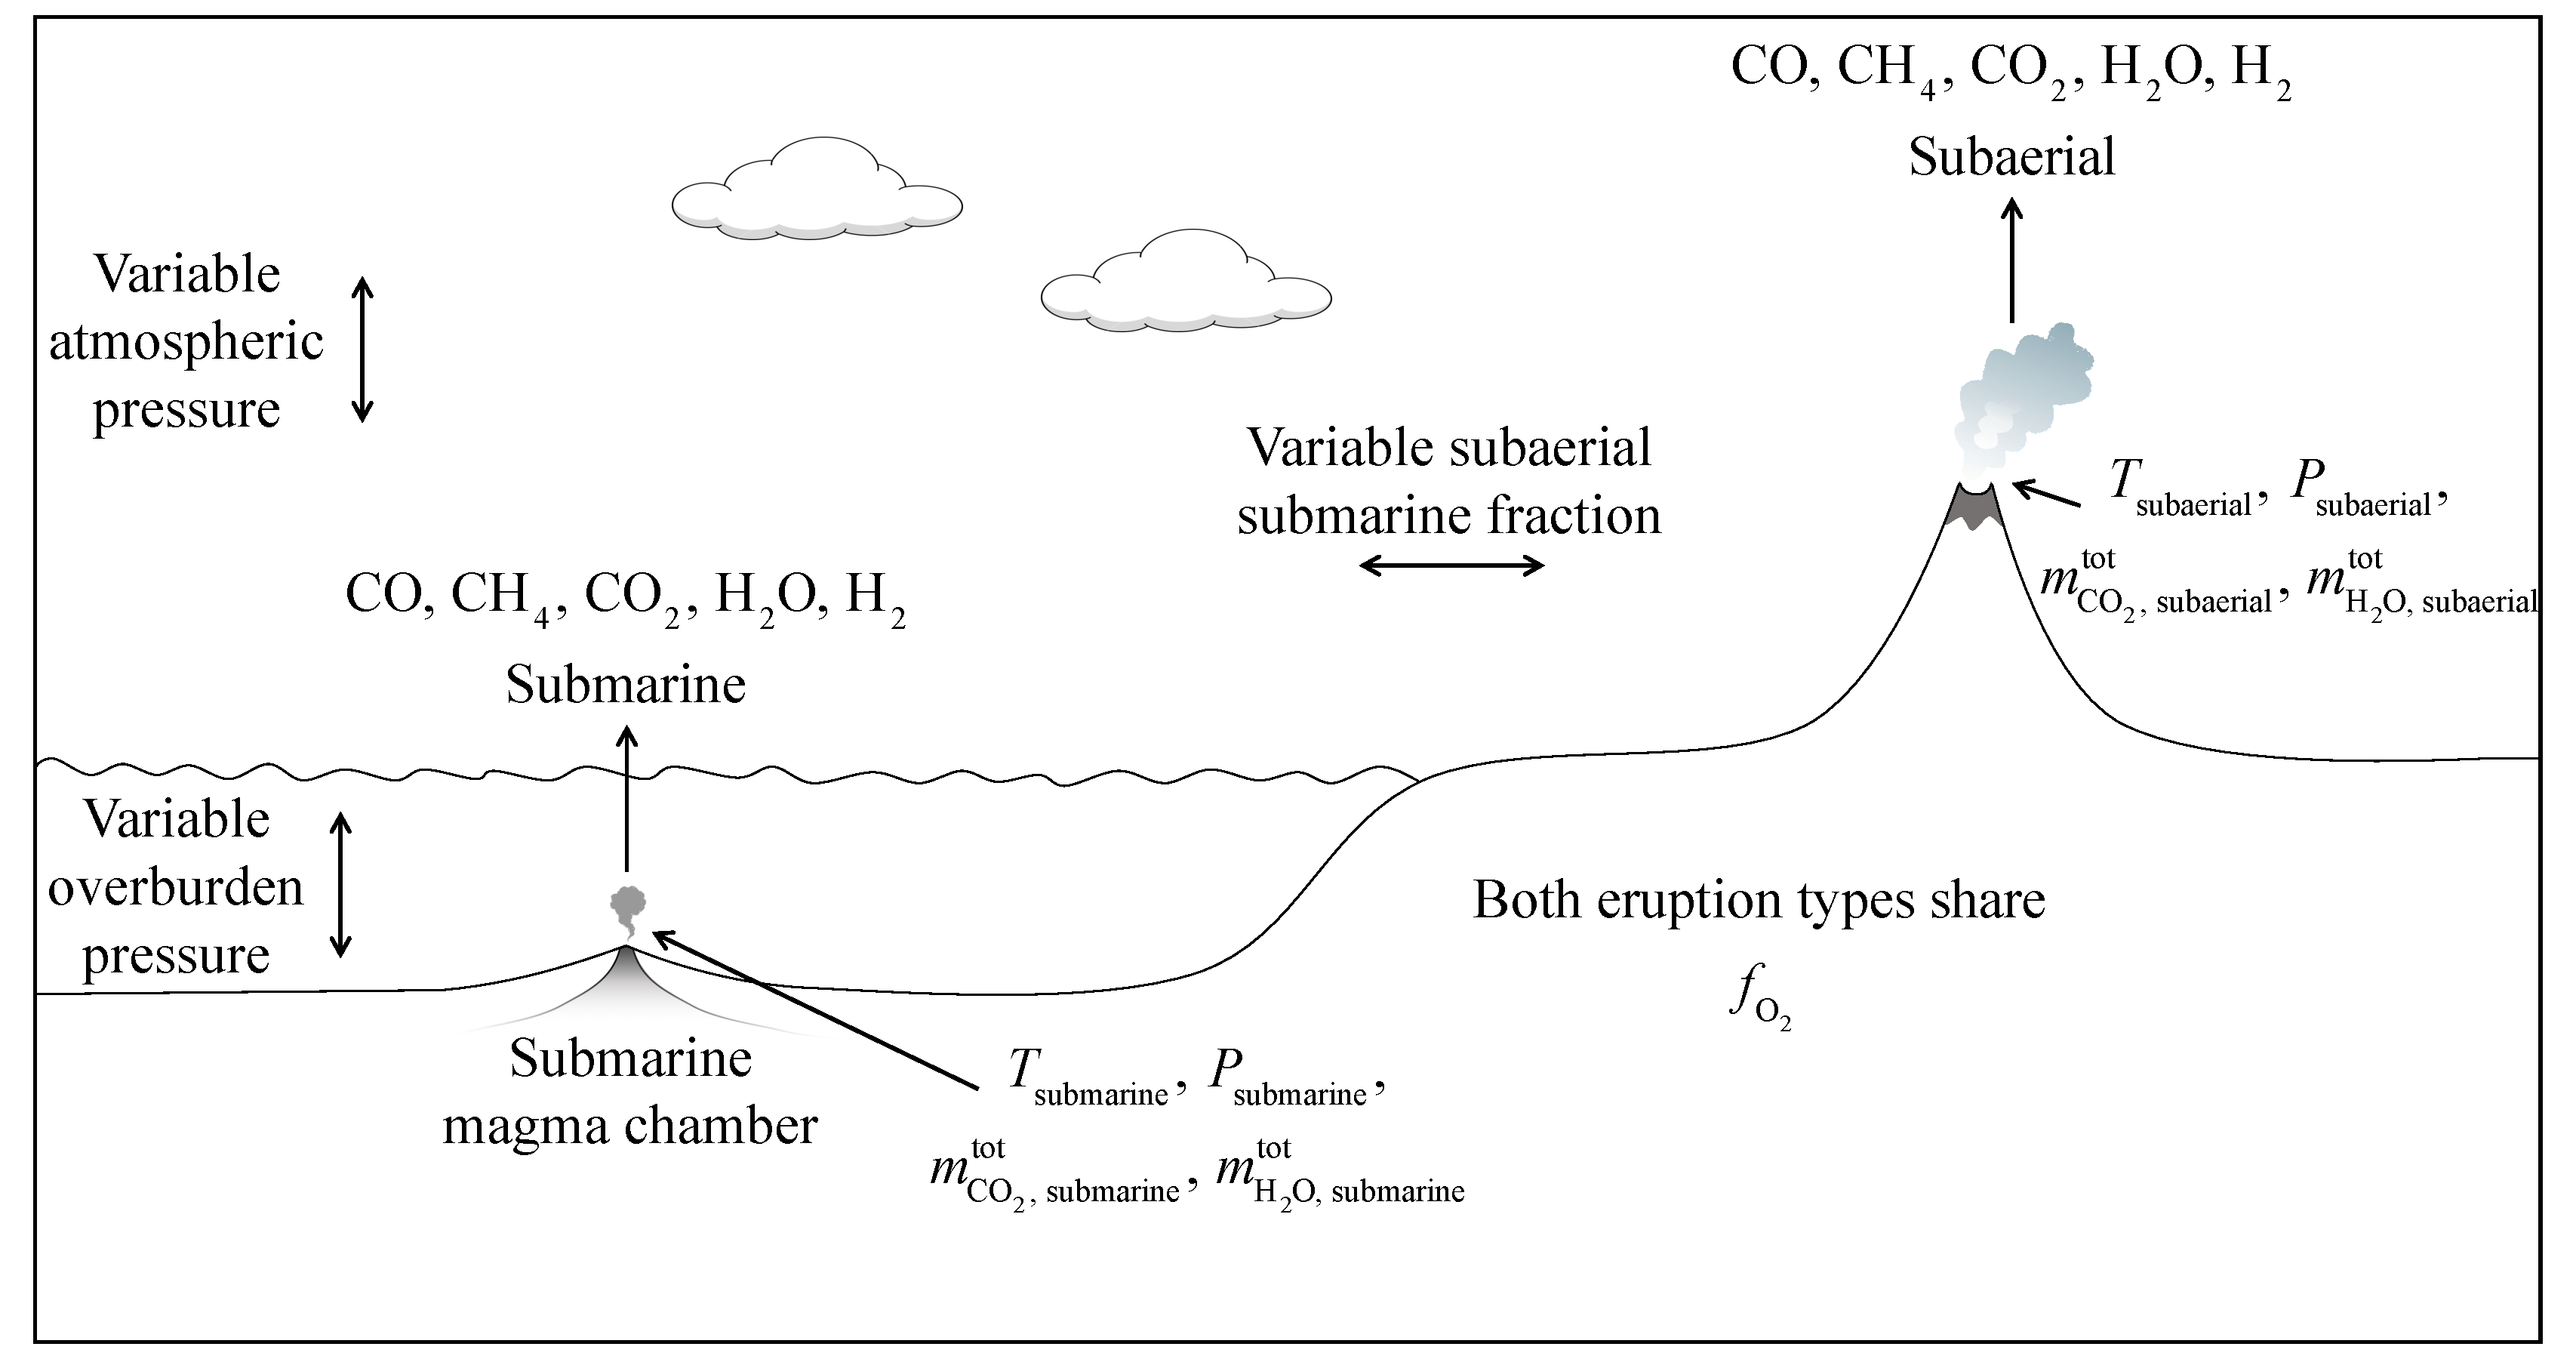
\includegraphics[width=\textwidth]{tex/3methane/figures/outgasing_diagram.pdf}
    \caption{Illustration of the parameters considered in the Monte-Carlo simulations.}
    \label{fig:digram}
\end{figure*}

\begin{table}
\caption{Monte-Carlo sampling distributions}
\label{tab:range}
\centering
\begin{tabularx}{0.95\linewidth}{p{0.15\linewidth} p{0.1\linewidth} p{0.1\linewidth} p{0.1\linewidth} p{0.4\linewidth}}
\hline \hline
  Variable & Low & High & Sampling method & Justification   \\
\hline
$T_\mathrm{submarine}$& 873 K & 1973 K   & linear uniform  & Range of submarine magma temperatures observed on Earth$^a$\\
$T_\mathrm{subaerial}$ & 873 K & 1973 K   & linear uniform  & Range of subaerial magma temperatures observed on Earth$^a$\\
$P_\mathrm{submarine}$ & 100 bar & 1000 bar  & linear uniform  & Degassing pressure at 1 km to 10 km ocean depth$^b$\\
$P_\mathrm{subaerial}$ & 0.001 bar & 100 bar  & log$_{10}$ uniform &    Rough range of subaerial degassing pressure in solar system \\
$m_\mathrm{CO_2,\:submarine}^\mathrm{tot}$ & $10^{-5}$ & $10^{-2}$ & log$_{10}$ uniform & Approx. CO$_2$ mass fraction range in Earth magma \citep{Wallace_2015,Wallace_2005,Anderson_2017,LeVoyer_2017} \\
$m_\mathrm{CO_2,\:subaerial}^\mathrm{tot}$ & $10^{-5}$ & $10^{-2}$   & log$_{10}$ uniform & Approx. CO$_2$ mass fraction range in Earth magma \citep{Wallace_2015,Wallace_2005,Anderson_2017,LeVoyer_2017}\\
$m_\mathrm{H_2O,\:submarine}^\mathrm{tot}$ & $10^{-5}$ & $10^{-1}$   & log$_{10}$ uniform & H$_2$O mass fraction range for Earth submarine outgassing \citep{Wallace_2015} \\
$m_\mathrm{H_2O,\:subaerial}^\mathrm{tot}$ & $10^{-5}$ & $10^{-1}$   & log$_{10}$ uniform & H$_2$O mass fraction range for Earth subaerial outgassing \citep{Wallace_2015} \\
$f_\mathrm{O_2}$ & FMQ-4 & FMQ+5   & log$_{10}$ uniform & Oxygen fugacity of most reducing Martian meteorite \citep{Catling_2017} to most oxidized magma on Earth \citep{Stamper_2014}$^c$ \\
$X$ & 0     & 1   & linear uniform & 0\% to 100\% subaerial volcanism\\
\hline
\multicolumn{5}{>{\raggedright\arraybackslash}p{\textwidth}}{
$^a$Coldest rhyolite magma, and hottest komatiites magmas \citep{Huppert_1984}

$^b$Assumes Earth's gravity. The solubility of H$_2$O in magma does not allow for significant CH$_4$ degassing at pressures greater than 1000 bar, equivalent to a depth of 10 km. 

$^c$FMQ is the fayalite-magnetite-quartz mineral redox buffer. See Chapter 7 in \citet{Catling_2017} for a description of mineral redox buffers. We use the parameterization for the FMQ buffer defined by \citet{Wones_1969}. This parameterization has only been experimentally validated to 1400 K \citep{ONeill_1987}, but we extrapolate using the parameterization to 1973 K}.
\end{tabularx}
\end{table}

To explore volcanism on Earth-like planets, we calculate outgassing speciation 10,000 times. For each calculation, we sample either uniform or log$_{10}$-uniform distributions (See Table \ref{tab:range}) of 10 parameters: $T_\mathrm{submarine}$, $P_\mathrm{submarine}$, $m_\mathrm{CO_2, \:\mathrm{submarine}}^{\mathrm{tot}}$, $m_\mathrm{H_2O, \:\mathrm{submarine}}^{\mathrm{tot}}$, $T_\mathrm{subaerial}$, $P_\mathrm{subaerial}$, $m_\mathrm{CO_2,\: \mathrm{subaerial}}^{\mathrm{tot}}$, $m_\mathrm{H_2O,\: \mathrm{subaerial}}^{\mathrm{tot}}$, $f_\mathrm{O_2}$, and $X$ . The width of each uniform sampling distribution are given and explained in Table \ref{tab:range}. We use inputs with subscripts “subaerial” to calculate subaerial volcanic speciation and inputs with subscripts “submarine” to calculate submarine volcanic speciation, and then we combine the results of each calculation with the formula
\begin{equation}
    {n_i} = \frac{{{P_{i{\text{, subaerial}}}}}}{{{P_{\text{subaerial}}}}}X + \frac{{{P_{i{\text{, submarine}}}}}}{{{P_{\text{submarine}}}}}(1 - X)
\end{equation}
Here, $n_i$ is the mixing ratio of averaged outgassed volatiles of species $i$ produced by the combination of subaerial and submarine volcanoes and $X$ is the fraction of subaerial volcanism ($0<X<1$). Also, $P_{i,\mathrm{\:subaerial}}$ and $P_{i,\mathrm{\: submarine}}$ are the partial pressure of species $i$ in subaerial and submarine outgassing, respectively.

To investigate volcanism on an ocean-world, we also calculate outgassing speciation 10,000 times. For each calculation, we sample either uniform or log$_{10}$-uniform distributions of inputs $T_\text{submarine}$, $P_\text{submarine}$ , $m_\mathrm{CO_2, \text{ submarine}}^{\mathrm{tot}}$, $m_\mathrm{H_2O, \text{ submarine}}^{\mathrm{tot}}$, and $f_\mathrm{O_2}$ with ranges defined and justified in Table \ref{tab:range}.

\subsection{Photochemical modeling: Uninhabited anoxic ocean-world with reducing volcanic gases}\label{method:photo}
We further investigate the CH$_4$+CO$_2$ biosignature by modeling the atmospheric composition of hypothetical uninhabited ocean-worlds with reducing volcanic gases. We consider planets orbiting the Sun, and a late M star - the latter because planets orbiting M-dwarfs are the most feasible targets for near-term telescopes like JWST \citep{Barstow_2016}.	Additionally, we simulate ocean-worlds because ocean-bottom degassing is most thermodynamically prone to produce CH$_4$, as revealed by our Monte-Carlo simulations and previous studies \citep{Kasting1998,French_1966} (see Section \ref{sec:water_solu} for further discussion).

To simulate atmospheres on uninhabited planets, we use the 1-D photochemical model contained within the open source software package \textit{Atmos}. \textit{Atmos} is derived from a model originally developed by the Kasting group \citep{Pavlov_2001}, and versions of this code have been used to simulate the Archean and Proterozoic Earth atmosphere \citep{Zahnle_2006}, Mars \citep{Sholes_2019,Smith_2014,Zahnle_2008}, and exoplanet atmospheres \citep{Harman_2015,Schwieterman_2019}. 

\section{Results}

\subsection{Monte-Carlo simulations}
\begin{figure*}
  \centering
  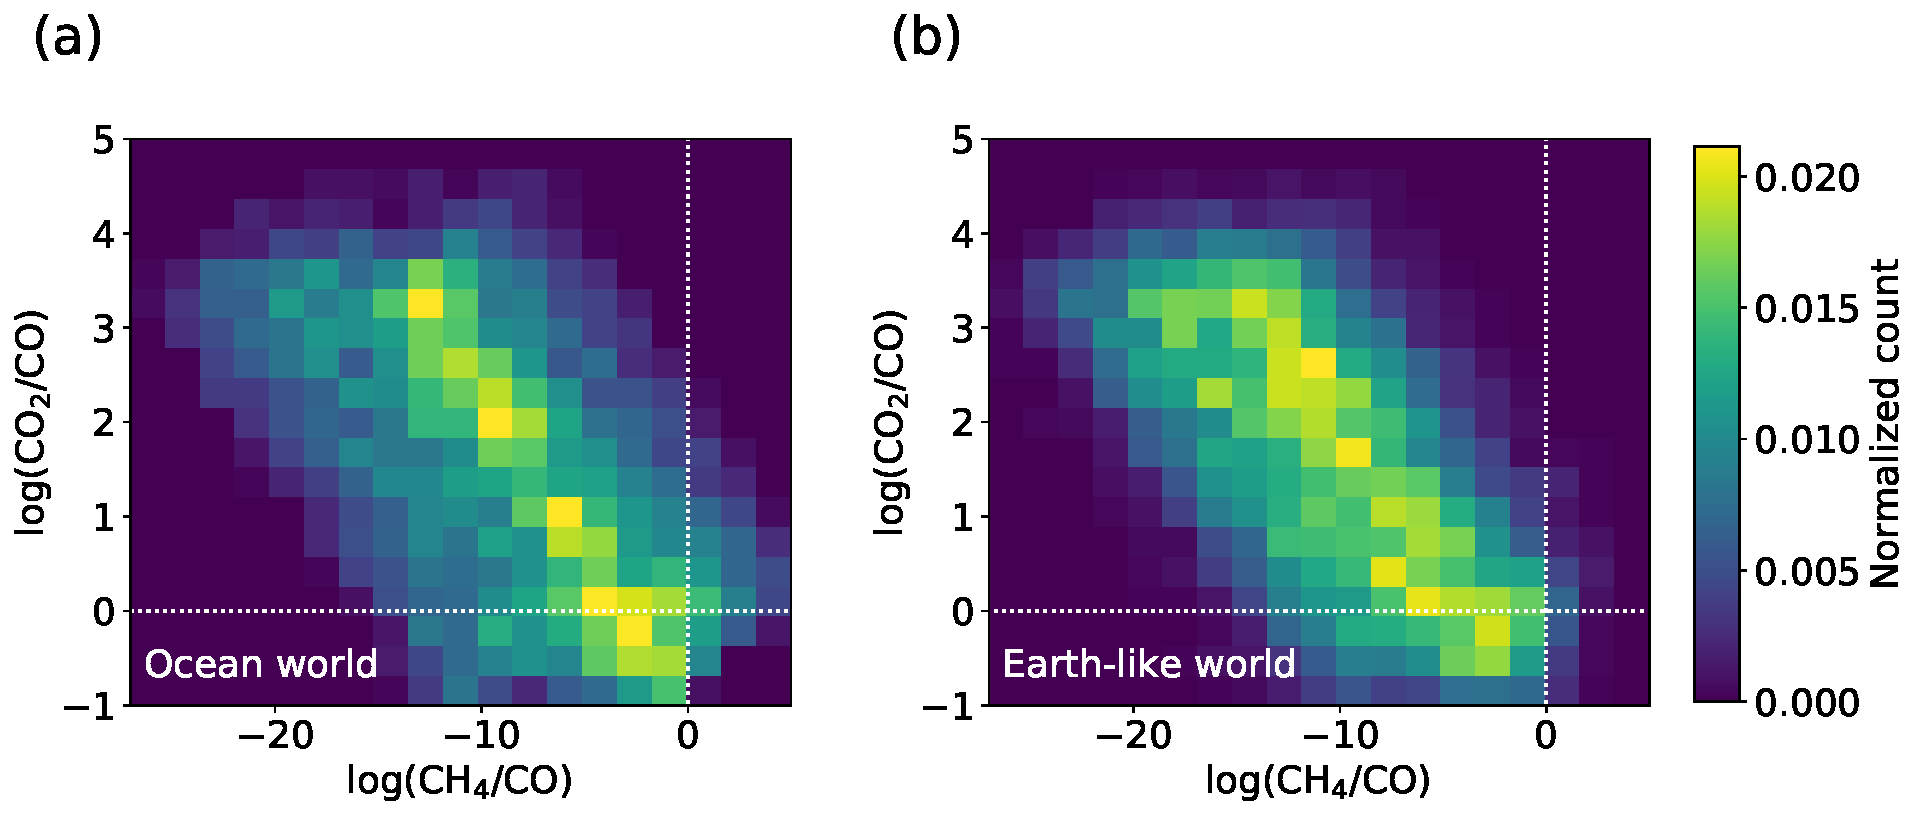
\includegraphics[width=\textwidth]{tex/3methane/figures/both.pdf}
  \caption{Results of the Monte-Carlo simulation described in Section 2.2. (a) and (b) show normalized count as a function of $\log(\mathrm{CH_4/CO})$ and $\log(\mathrm{CO_2/CO})$ for an ocean world and Earth-like world, respectively. The white dotted lines indicate where CH$_4$/CO = 1 and CO$_2$/CO = 1. For almost all calculated gas speciations, CO$_2$ and CO are much more abundant than CH$_4$.}
  \label{fig:result1}
\end{figure*}

Figure \ref{fig:result1} shows joint distributions of gas ratios CH$_4$/CO and CO$_2$/CO from the Monte-Carlo simulation described in Section \ref{sec:monte}. These results suggest that for most combinations of parameters volcanoes are most likely to produce more CO$_2$ than CO, and negligible CH$_4$, which is the case for the modern Earth \citep{Catling_2017}. About 7\% and 2\% of calculations produce more CH$_4$ than CO for ocean worlds and Earth-like worlds, respectfully. In the vast majority of cases, either CO or CO$_2$ is the dominant carbon-bearing species.

Figure \ref{fig:CH4}a and \ref{fig:CH4}b show CH$_4$ production from the Monte-Carlo simulations in terms of mol CH$_4$/kg magma. To give a sense for the gas fluxes implied by these CH$_4$ productions, we multiply the distributions in Figure \ref{fig:CH4}a and \ref{fig:CH4}b by the magma production rate of modern Earth of $9\times10^{13}$ kg/yr \citep{Crisp_1984}, which gives the gas fluxes shown in Figure \ref{fig:CH4}c and \ref{fig:CH4}d, respectively. About 0.1\% of calculations predict more than 10 Tmol CH$_4$/yr for both Earth-like worlds and ocean worlds. This small fraction suggests that for modern Earth magma production rates, volcanoes are unlikely to produce CH$_4$ fluxes comparable to modern Earth's biological flux of 30 Tmol/yr \citep{Hauglustaine_2007}.

Magma production rates larger than modern Earth's increase the probability that volcanic fluxes of CH$_4$ become comparable to biological CH$_4$ fluxes. For example, the early Archean Earth could have had magma production rates up to about 25 times modern Earth's \citep{Sleep_2001}. Such a magma production rate would shift the distributions in Figure \ref{fig:CH4}c and \ref{fig:CH4}d to larger values by a factor of 25 (or in log$_{10}$-space, by a factor of 1.4). In this case, $\sim$2\% of calculations (for either Earth-like world or ocean world) would predict more than 10 Tmol CH$_4$/yr. 

Crucially, large CH$_4$ fluxes should almost always coincide with even larger CO fluxes (horizontal axis in Figure \ref{fig:result1}). Therefore, the unlikely cases where volcanoes mimic biological CH$_4$ fluxes can be identified by detecting abundant CO in a planet's atmosphere. We further investigate CO as a CH$_4$+CO$_2$ biosignature discriminant using a photochemical model in the following section.

\begin{figure*}
  \centering
  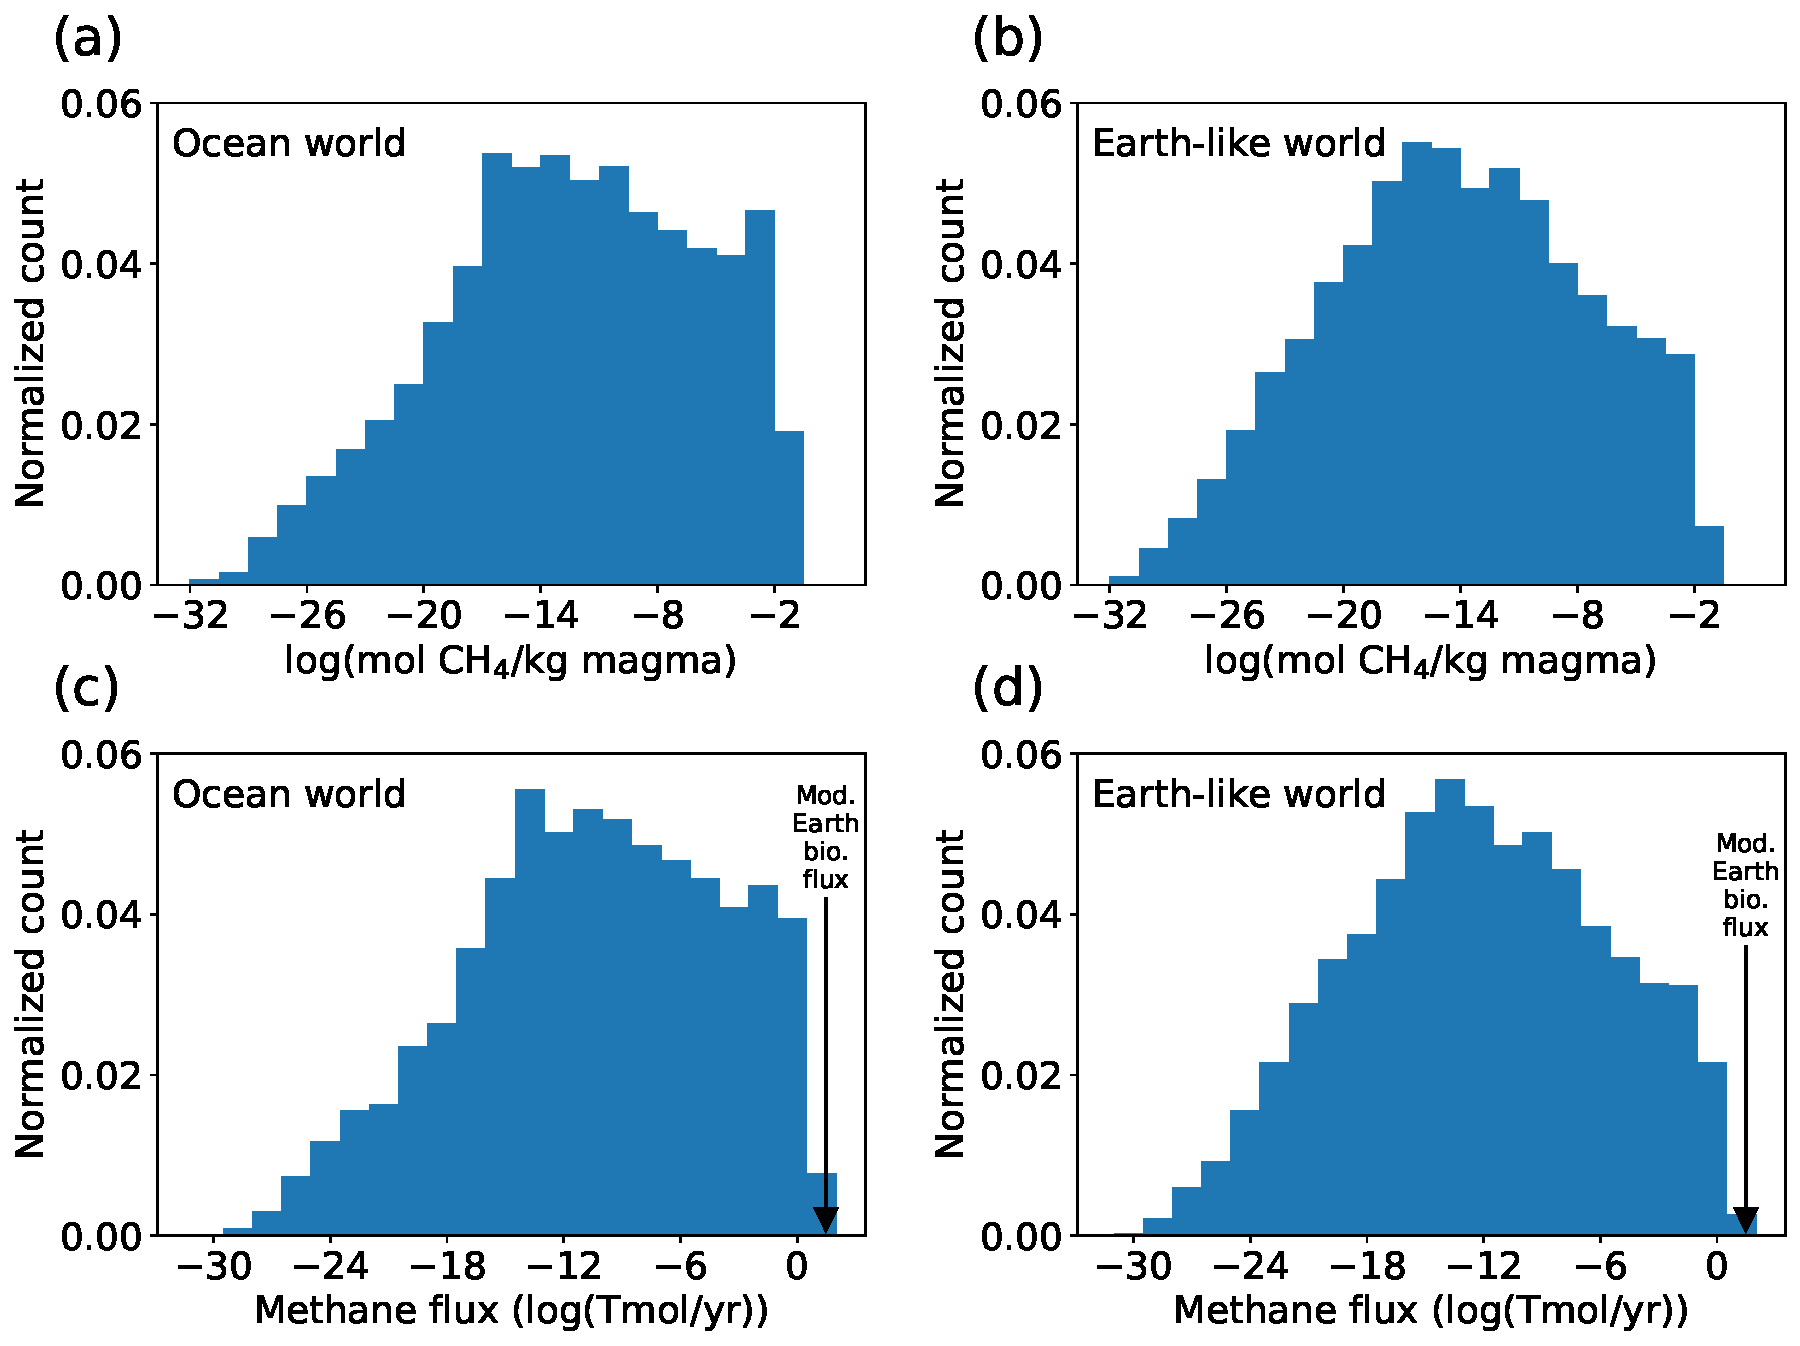
\includegraphics[width=\textwidth]{tex/3methane/figures/CH4_prod.pdf}
  \caption{Normalized count of methane production (mol gas/kg magma) for (a) ocean worlds and (b) Earth-like worlds. Distributions were calculated by sampling the ranges in Table \ref{tab:range}. Multiplying Earth's magma production rate of $9\times10^{13}$ kg magma/yr by (a) and (b) gives the methane fluxes in (c) and (d), respectively. For modern Earth's magma production rate, volcanoes are likely to produce negligible CH$_4$.}
  \label{fig:CH4}
\end{figure*}

\subsection{Photochemical modeling: Uninhabited anoxic ocean-world with reducing volcanic gases}\label{sec:photochem}

\begin{figure*}
  \centering
  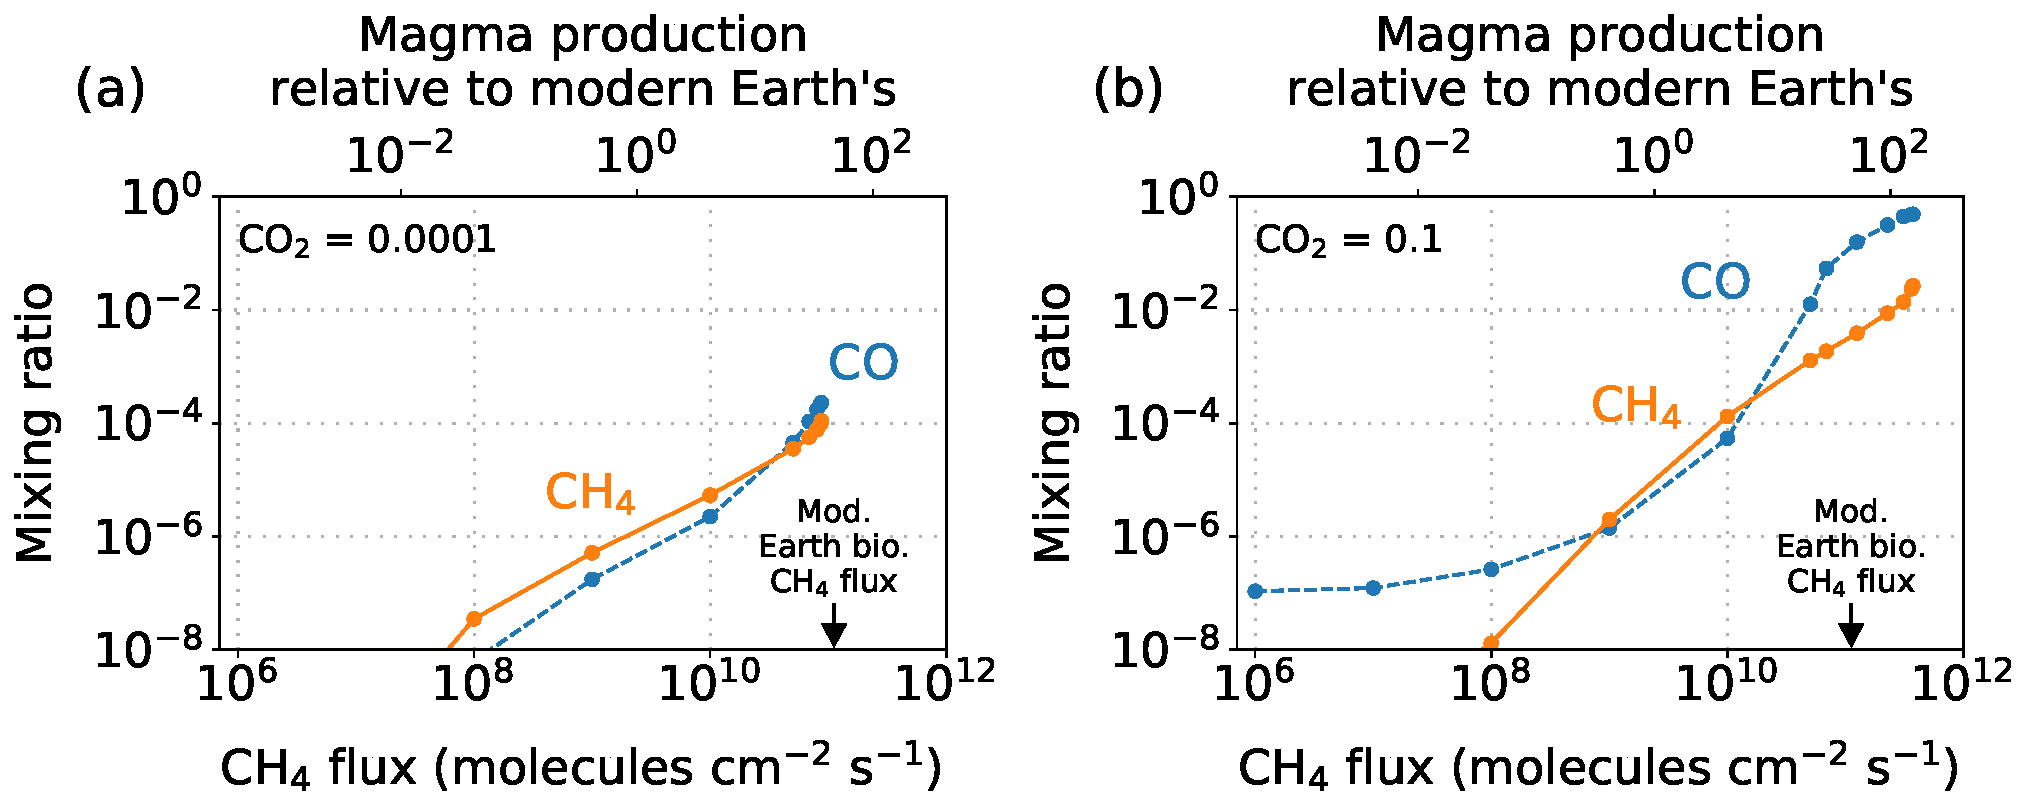
\includegraphics[width=\textwidth]{tex/3methane/figures/Figure4.pdf}
  \caption{Atmospheric mixing ratios of CO and CH$_4$ as a function of magma production rate relative to modern Earth's (or CH$_4$ flux) on an anoxic ocean-world with reducing volcanic gases orbiting a sun-like star. (a) and (b) are identical model runs, except (a) assumes a constant atmospheric CO$_2$ mixing ratio of 0.0001, and (b) assumes a constant atmospheric CO$_2$ mixing ratio of 0.1. Modern Earth's biological CH$_4$ flux is indicated on the horizontal axes. Archean Earth-like CH$_4$ fluxes and abundances are only mimicked by volcanoes for magma production rates $>$10 times modern Earth's. Such false-positive cases can be distinguished from biology because the CO abundance exceeds the CH$_4$ abundance, which would likely not be the case for an inhabited planet.}
  \label{fig:photosun}
\end{figure*}

We use the \textit{Atmos} photochemical model to simulate the potential observable gas abundances of uninhabited Earth-sized ocean-worlds with reducing volcanic gases. We consider such planets because they are the most prone to mimic biology by producing volcanic CH$_4$ (see Section \ref{sec:water_solu} for more details). Our hypothetical planets have 1 bar N$_2$ dominated atmospheres, 400 bars of ocean water, magma degassing at 1473 K and mantle redox states of FMQ-4. Here, FMQ is the fayalite-magnetite-quartz buffer which is a synthetic reference $f_\mathrm{O_2}$ value at fixed temperature-pressure conditions. Additionally, we assume that the magma contains 0.1 wt\% CO$_2$, and 1 wt\% H$_2$O. Our assumed H$_2$O concentration is comparable to those observed in submarine hot-spot magmas (0.2 to 1.5 wt\%) \citep{Wallace_2015}, however, the CO$_2$ concentration we assume is slightly lower \citep{Anderson_2017}. Given these inputs, our speciation model (Section \ref{sec:volcmodel}) predicts gas production from erupted magma of $q_\mathrm{H_2} = 4.36\times 10^{-2}$ mol gas/kg magma, $q_\mathrm{CO} = 1.29\times 10^{-2}$ mol gas/kg magma, and $q_\mathrm{CH_4} = 7.39\times 10^{-3}$ mol gas/kg magma.

The magnitude of gas fluxes to the atmosphere resulting from chemically reducing volcanism depends on the magma production rate (Equation \eqref{eq:Flux}). We consider magma production rates between about $10^{-3}$ and $10^2$ Earth’s modern magma production rate of $9\times10^{13}$ kg magma/yr \citep{Crisp_1984}. 

For each magma production rate, we calculate the outgassing flux of CH$_4$, H$_2$, and CO and set these fluxes as lower boundary conditions to the \textit{Atmos} photochemical model (the outgassing model also gives CO$_2$ and H$_2$O fluxes, but we don't use them in our photochemical modeling). \textit{Atmos} only allows fixed CO$_2$ mixing ratios and not CO$_2$ fluxes so we consider cases with low and high CO$_2$ (100 ppm and 10\%). Additionally, we set the deposition velocity of CO to $10^{-8}$ cm s$^{-2}$ to reflect the abiotic uptake of CO by the ocean \citep{Kharecha_2005}. All other boundary conditions are specified in Chapter Appendix \ref{sec:photo_boundary_cond}. Given volcanic outgassing fluxes and other boundary conditions, \textit{Atmos} calculates the mixing ratios of all species when the atmosphere is at photochemical equilibrium.

Figure \ref{fig:photosun} shows the photochemical modeling results of reducing volcanic gases on an uninhabited Earth-sized ocean-world orbiting the Sun. Figure \ref{fig:photosun}a assumes that the atmosphere has 100 ppmv CO$_2$ while Figure \ref{fig:photosun}b assumes that atmospheric CO$_2$ is 10\%. Carbon monoxide and methane are more abundant in the model with more CO$_2$ because CO$_2$ shields the lower atmosphere from hydoxyl (OH) production from water photolysis. In anoxic atmospheres, OH is a significant sink for both CO and CH$_4$ through the reactions $\mathrm{CO_2}+\mathrm{OH}\rightarrow \mathrm{CO_2}+\mathrm{H}$ and $\mathrm{CH_4}+\mathrm{OH}\rightarrow \mathrm{CH_3}+\mathrm{H_2O}$. OH is generated primarily from H$_2$O photolysis ($\mathrm{H_2O}+h \nu [\lambda<200 \:\mathrm{nm}]\rightarrow \mathrm{OH}+\mathrm{H}$), but CO$_2$ shields H$_2$O from photolysis in model runs with 10\% CO$_2$, thus limiting the CH$_4$ and CO destruction from OH. Also, CH$_4$ is more abundant in atmospheres with more CO$_2$ because CO$_2$ shields CH$_4$ from direct photolysis in cases when CO$_2$ is $>$200 times as abundant as CH$_4$. This factor of $\sim$200 comes from comparing Lyman-$\alpha$ ($\lambda=121.6$ nm) CO$_2$ and CH$_4$ cross sections. Lyman-$\alpha$ is the portion of the UV spectrum primarily responsible for photolyzing CH$_4$.

Figure \ref{fig:photosun} suggests that reducing volcanic gases on an ocean world orbiting a sun-like star will only mimic biological CH$_4$ fluxes and abundances for large magma production rates. Volcanism can generate Earth’s modern biological CH$_4$ flux when the magma production rate is $\sim$50 times modern Earth’s (Figure \ref{fig:photosun}). In this case, the photochemical model predicts an atmospheric CH$_4$ abundance between 0.01\% and 0.3\%, depending on the CO$_2$ mixing ratio. Such CH$_4$ abundances are similar to the 0.01\% to 1\% expected in the early Archean Earth atmosphere \citep{Catling_2020}. In contrast, magma production rates comparable to the modern Earth's result in a CH$_4$ flux of $2.4\times 10^9$ molecules cm$^{-2}$ s$^{-1}$ (0.64 Tmol/yr) and CH$_4$ abundances $<30$ ppm, which are likely to be considered abiotic levels in an anoxic atmosphere.

\begin{figure*}
  \centering
  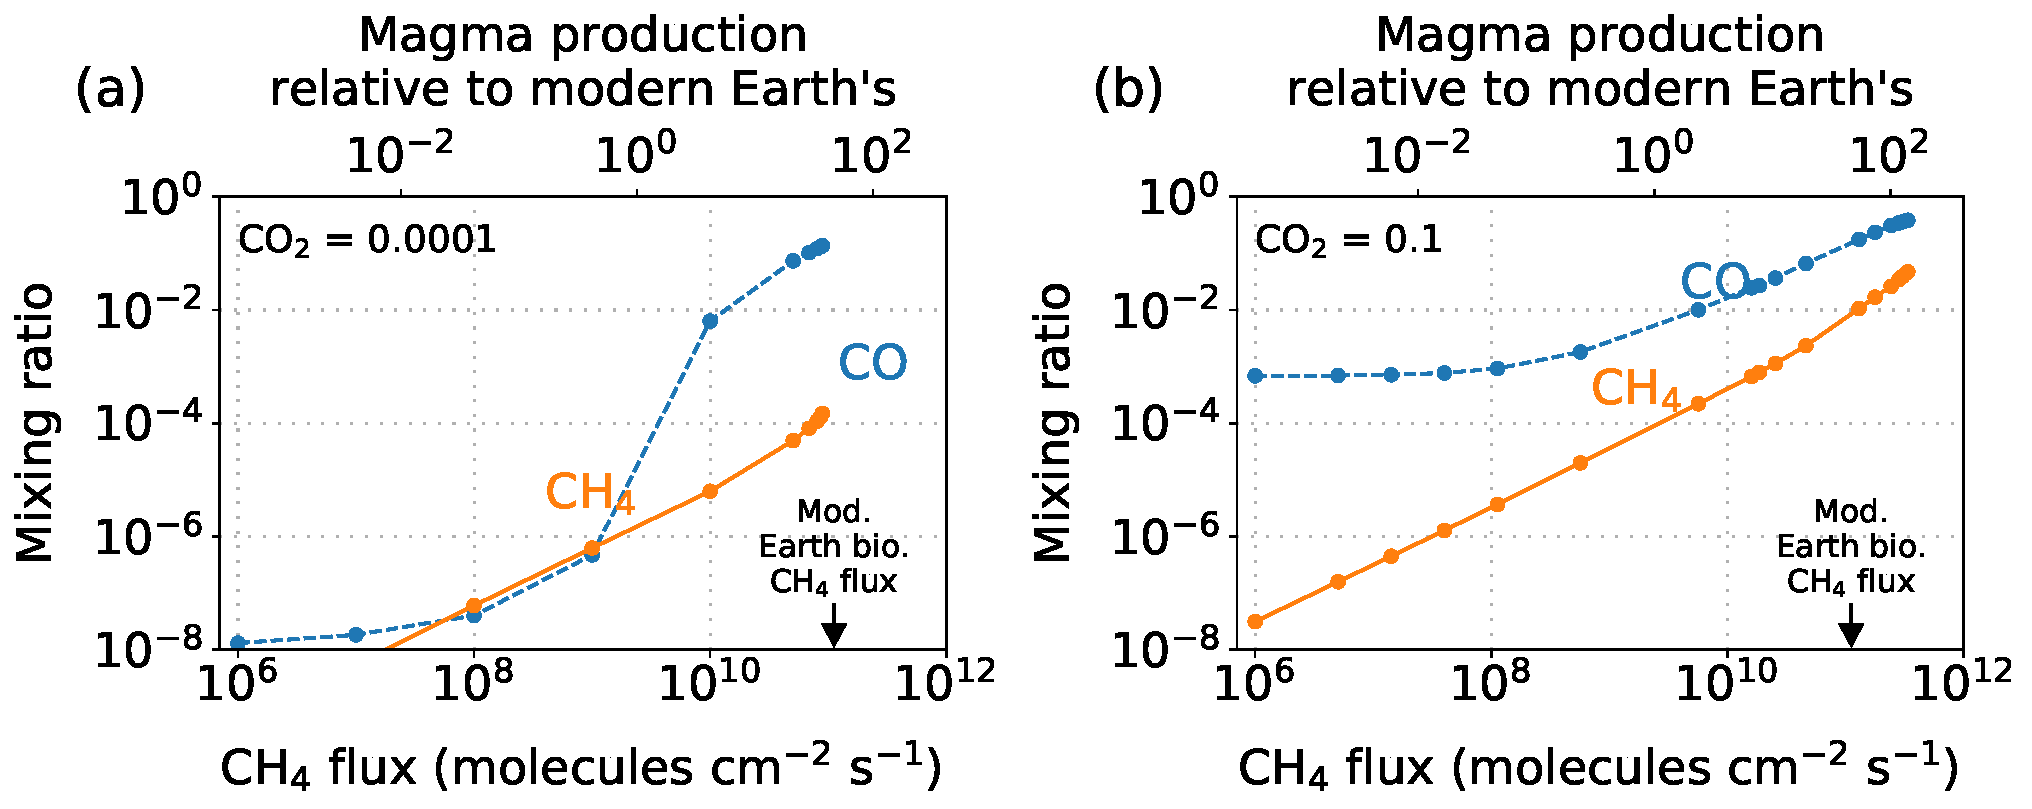
\includegraphics[width=\textwidth]{tex/3methane/figures/Figure5.pdf}
  \caption{Identical to Figure \ref{fig:photosun}, except for a planet that orbits a M8V star instead of a sun-like star.}
  \label{fig:photoM}
\end{figure*}

Figure \ref{fig:photoM} shows the CO and CH$_4$ mixing ratios on an Earth-sized ocean-world with reducing volcanic gases orbiting a cold M star. CO and CH$_4$ are more abundant on the ocean-world orbiting the M star compared to the ocean-world orbiting a Sun-like star (Figure \ref{fig:photosun}). This is because M8V stars have a low flux of near-ultraviolet radiation compared to sun-like stars. The low near-ultraviolet flux reduces OH produce from H$_2$O photolysis, thus allowing for relatively high CO and CH$_4$ concentrations. 

One consequence of M-dwarf photochemistry is a higher likelihood of Archean Earth-like CH$_4$ abundances on uninhabited planets with reducing gases from volcanism. Figure \ref{fig:photoM} shows that modern Earth magma production rates can result in CH$_4$ abundances up to 0.01\% which is comparable to what is expected in the Archean atmosphere. 

Potential CH$_4$ biosignature false positives from reducing volcanic gases might be discriminated from inhabited worlds using observations of CO. For planets orbiting Sun-like stars (Figure \ref{fig:photosun}) or M stars (Figure \ref{fig:photoM}) the CO abundance is higher than the CH$_4$ abundance in every case that is a potential outgassing false-positive. Some authors have argued that a large CO abundance is unlikely on an inhabited planet, because atmospheric CO should be readily consumed by biology \citep{Krissansen-Totton_2018a}. Conversely, \citet{Schwieterman_2019} has demonstrated hypothetical cases where large CO can coincide with with biology in an anoxic atmosphere. We further discuss CO as a false-positive discriminant in Section \ref{sec:CO_disc}.

\section{Discussion}

\subsection{The reasons why volcanoes produce little CH$_4$} \label{sec:littleCH4}

Our modeling results show that for modern Earth magma production rates, volcanic fluxes of reducing gases are unlikely to produce more than 1 Tmol CH$_4$/yr even in an extreme case (Figure \ref{fig:CH4}). This flux is relatively small compared to the flux of other volcanic gases on modern Earth. For example, Earth's modern volcanoes produce about ~7.5 Tmol CO$_2$/yr and ~95 Tmol H$_2$O/yr \citep[p. 203]{Catling_2017}. There are three main reasons why the outgassing model predicts little CH$_4$, which we discuss below.

\subsubsection{Volcanoes produce little CH$_4$ because of water solubility in magma} \label{sec:water_solu}

One reason for small CH$_4$ outgassing is the high solubility of water in magma at high pressures. Consider Equation \eqref{eq:react3}, which can be re-arranged to the following
\begin{equation}\label{eq:react3.1}
    \frac{P_{\mathrm{CH_4}}}{P_{\mathrm{CO_2}}}=\frac{K_3 P_\mathrm{H_2O}^2}{f_\mathrm{O_2}^2}
\end{equation}
The ratio $P_{\mathrm{CH_4}}/P_{\mathrm{CO_2}}$ in a gas bubble in magma is directly proportional to $P_\mathrm{H_2O}^2$ within that bubble. Generally speaking, $P_\mathrm{H_2O}$ increases as the total pressure of degassing increases because all partial pressures must sum to the total pressure (Equation \eqref{eq:pres}). For example, subaerial degassing at $\sim$1 bar will have a relatively small $P_\mathrm{H_2O}$, and thus a small $P_{\mathrm{CH_4}}/P_{\mathrm{CO_2}}$ ratio. On the other hand, submarine degassing at $\sim$400 bar should have a larger H$_2$O partial pressure, and thus a larger $P_{\mathrm{CH_4}}/P_{\mathrm{CO_2}}$ ratio. Here, the equilibrium constant and oxygen fugacity have extremely weak pressure dependencies, i.e. they are effectively constant as degassing pressure changes.

\begin{figure*}
  \centering
  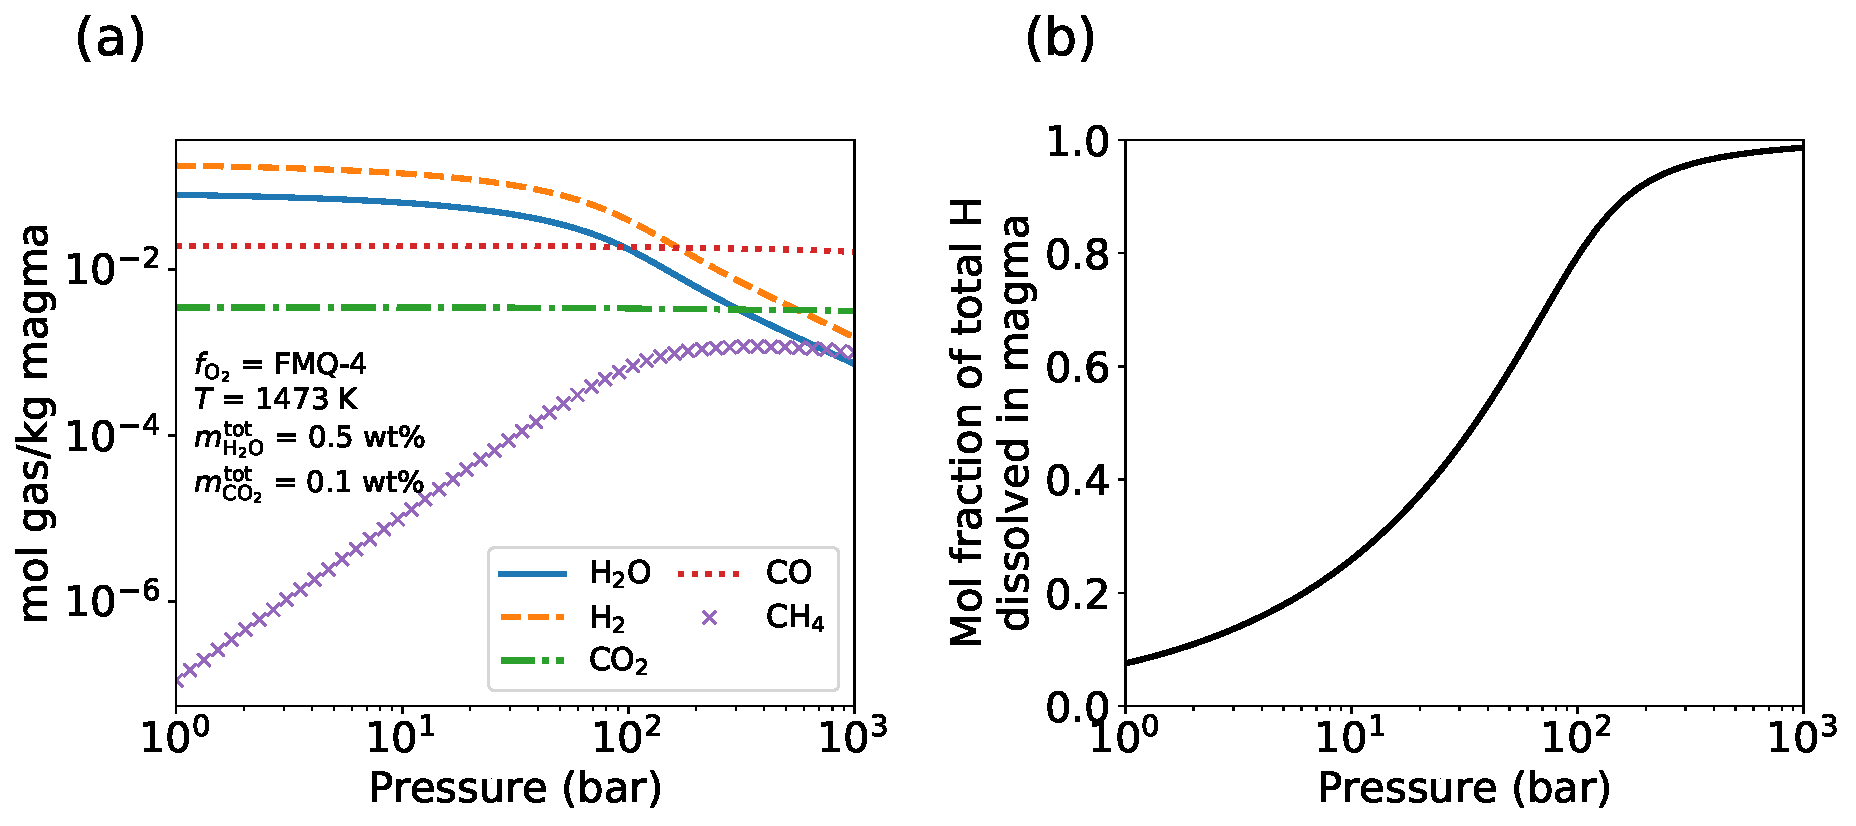
\includegraphics[width=\textwidth]{tex/3methane/figures/P_dependence.pdf}
  \caption{(a) Modeled gases speciation as a function of pressure. (b) Mole fraction of total hydrogen dissolved in the magma as a function of pressure. Model assumes $f_\mathrm{O_2}=$ FMQ-4, $T=1473$ K, $m_\mathrm{H_2O}^\mathrm{tot}$ = 0.5 wt\%, and $m_\mathrm{CO_2}^\mathrm{tot}$ = 0.1 wt\%. Methane becomes more prevalent in volcanic gases at higher pressures, but asymptotes because hydrogen dissolves into the magma, reducing the total amount of H-bearing volatiles released from the magma.}
  \label{fig:P_dependence}
\end{figure*}

Figure \ref{fig:P_dependence}a shows modeled gas speciation for highly reducing volcanism ($f_\mathrm{O_2}=$ FMQ-4) as a function of pressure. For small pressures ($<100$ bar), CH$_4$ increases with increasing pressure and then asymptotes for pressures $>100$ bar.

CH$_4$ asymptotes because of the high solubility of water in magma at high pressure. High pressures dissolve a large fraction of the total available hydrogen as H$_2$O into the magma, which is shown in Figure \ref{fig:P_dependence}b. Dissolving a large amount of H$_2$O into the magma limits the amount of hydrogen available in the gas phase for making H-bearing species, like CH$_4$, H$_2$O and H$_2$. 

In summary, high pressure is in some ways thermodynamically favorable for making methane because $P_{\mathrm{CH_4}}/P_{\mathrm{CO_2}} \propto P_\mathrm{H_2O}^2$, but also unfavorable because high pressure dissolves a large fraction of the available hydrogen in the magma as H$_2$O. Limited amounts of hydrogen in gas bubbles results in small amounts of CH$_4$ produced.

\citet{Kasting1998} used Equation \eqref{eq:react3.1} to argue that $\sim$1\% of the carbon outgassed by submarine volcanoes should be CH$_4$ for magma with $f_\mathrm{O_2} = \mathrm{FMQ}$. They assumed that $P_\mathrm{H_2O} \approx P$, the total pressure. This assumption is valid for oxidized subaerial volcanoes because $\sim$90\% of the gas exsolved by Earth's subaerial volcanoes is H$_2$O \citep[p. 203]{Catling_2017}. However, $P_\mathrm{H_2O} < P$ for submarine volcanoes because of the high-water solubility in magma at high pressure. Our outgassing model, which accounts for water's solubility in magma, produces negligible methane.

\citet{Li_2004} also predict abundant CH$_4$ produced by subaerial and submarine volcanoes (their Figure 5). However they calculated equilibrium constants in units of bars, but then used units of Pascals for equilibrium chemistry calculations. The result was that they calculated speciation for pressures a factor 10,000 times greater than reported. For example, we were able to reproduce their subaerial outgassing case (their Figure 5a) by assuming $P=10,000$ bar and not the $P=1$ bar total pressure they intended. Additionally, like \citet{Kasting1998}, they did not account for the high solubility of H$_2$O in magma at high pressure. Their methods assume the total hydrogen outgassed for submarine volcanoes is the same as the total hydrogen outgassed by subaerial volcanoes. This should not be the case because at high pressure water dissolves in magma and is unavailable for making H-bearing gas species (Figure \ref{fig:P_dependence}b).

The pressure dependence of volcanic outgassing has implications for planetary atmospheres generally \citep{Gaillard_2014}. Thin atmospheres will allow substantial degassing of both carbon and hydrogen bearing species. However, planets with thick atmospheres or large global oceans will have volcanic degassing dominated by CO$_2$ and CO, and almost no hydrogen bearing species. The overburden pressure where C-bearing species dominate depends primarily on the un-degassed concentrations of H$_2$O and CO$_2$ in the magma. In Figure \ref{fig:P_dependence}, CO$_2$ and CO overwhelms H-bearing species at $\sim$1000 bar for initial volatile concentrations of $m_\mathrm{CO_2}^\mathrm{tot} = 0.1$\%, and $m_\mathrm{H_2O}^\mathrm{tot} = 0.5$\%. In contrast, Figure 8 in \citet{Gaillard_2014} illustrates a case with less volatiles ($m_\mathrm{CO_2}^\mathrm{tot} = 0.007$\% and $m_\mathrm{H_2O}^\mathrm{tot} = 0.03$\%) where C-bearing species eclipse H-bearing species at $\sim$1 bar.

\subsubsection{Volcanoes produce little CH$_4$ because magma is hot}

Relatively little CH$_4$ is produced by volcanoes because CH$_4$ is generally not thermodynamically favorable at typical magma degassing temperatures. Figure \ref{fig:T_dep} shows gas speciation as a function of temperature for a submarine outgassing case. For these chosen inputs, CH$_4$ is the dominant carbon-bearing species for $T<1200$ K. Mid-ocean ridge basalts (MORB) are about 2/3 of total magma produced on Earth \citep{Crisp_1984}. MORB magma erupt at temperatures between 1473 K and 1650 K \citep{Scheidegger_1973} and are thus in a temperature regime where CH$_4$ is unfavorable even from more reducing volcanism.

\begin{figure}
    \centering
    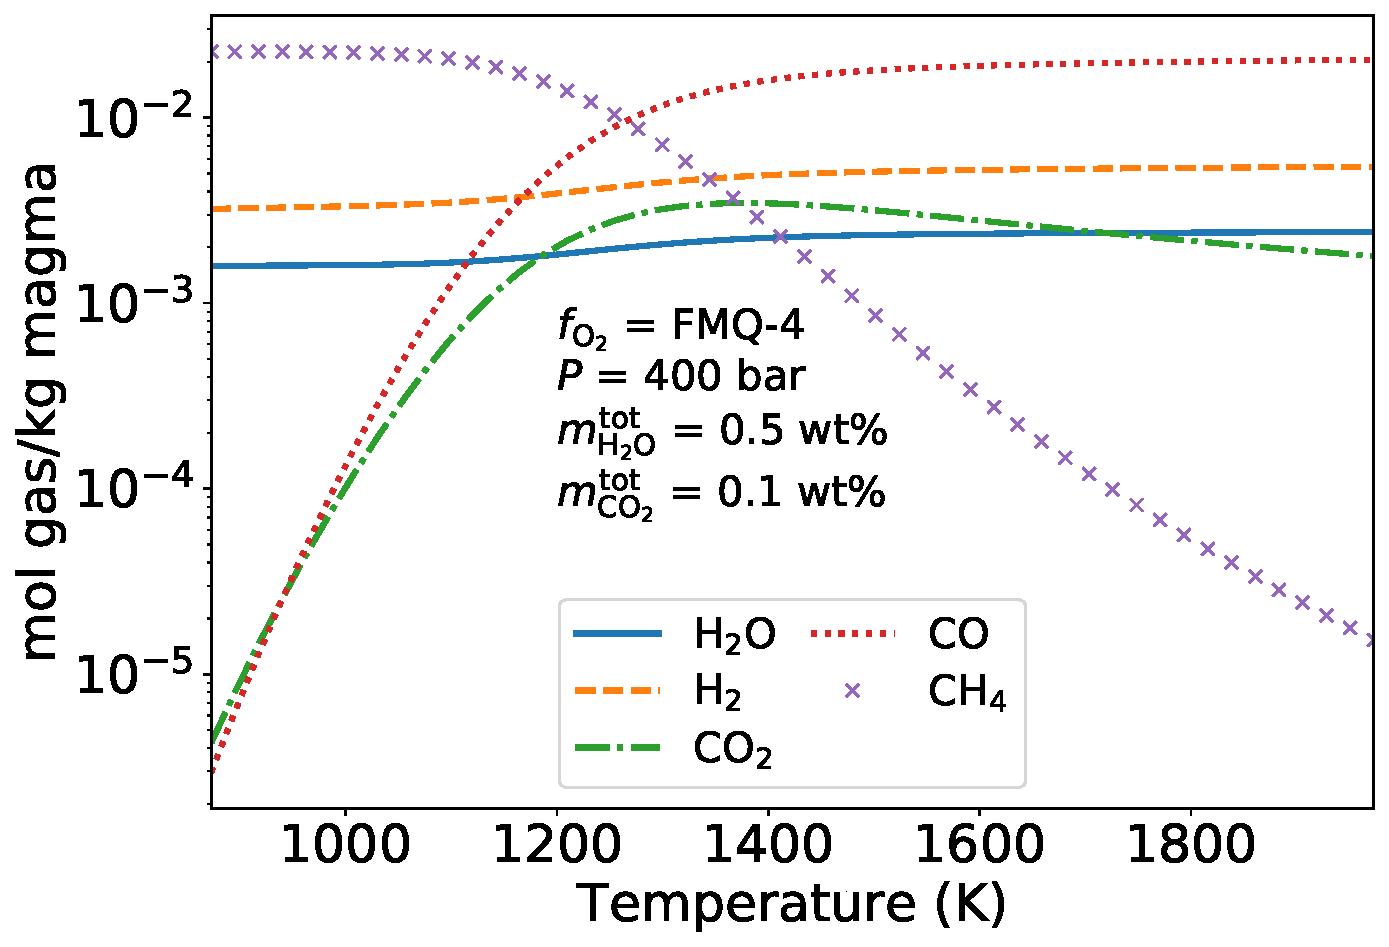
\includegraphics[width=10 cm]{tex/3methane/figures/T_dependence.pdf}
    \caption{Modeled volcanic outgassing speciation as a function of temperature. Model assumes $f_\mathrm{O_2}=$ FMQ-4, $P=400$ bar, $m_\mathrm{H_2O}^\mathrm{tot}$ = 0.5 wt\%, and $m_\mathrm{CO_2}^\mathrm{tot}$ = 0.1 wt\%. CH$_4$ is more thermodynamically favorable at lower degassing temperatures.}
    \label{fig:T_dep}
\end{figure}

On the other hand, magma from arc volcanoes is generally much colder than MORB magma. \citet{Moussallam_2019} report magma temperatures for many arc volcanoes (their Table S3), the coldest of which are 1123 K. Thus, it does seem possible for magma to be cold enough for CH$_4$ to be the dominant carbon-bearing outgassed species from an extremely reducing volcano with $f_\mathrm{O_2}=$ FMQ-4.

Recall that large magma production rates ($\sim$30x modern) are required for volcanoes to produce CH$_4$ fluxes compared to biological ones (Figure \ref{fig:photosun}). It seems unlikely that planets with large magma production rates will have magma temperatures cold enough to produce plentiful CH$_4$. For example, the Archean Earth may have had a larger magma production rate than the modern Earth because the Earth's mantle was hotter on the distant past \citep{Sleep_2001}. The hotter Archean mantle resulted in the eruption of $\sim$1800 K komatiite magmas \citep{Huppert_1984}, or possibly only $\sim$1600 K \citep{McKenzie_2020}. Such hot magma degassing is unfavorable for methane (Figure \ref{fig:T_dep}).

\subsubsection{Volcanoes produce little CH$_4$ because very low oxygen fugacity is required}

The final reason why volcanic CH$_4$ is unlikely on terrestrial planets is because very low $f_\mathrm{O_2}$ is required to make abundant methane. Figure \ref{fig:fO2} shows gas speciation as a function of oxygen fugacity for submarine volcanism. For these assumed inputs, methane is a substantial fraction of outgassed species for $f_\mathrm{O_2}<$ FMQ-3, and at FMQ-5 (roughly equivalent to the quartz-fayalite-iron buffer) half the carbon is converted to CH$_4$, while the other half is CO. Most degassing on Earth occurs at approximately $f_\mathrm{O_2}=\mathrm{FMQ}$ \citep[p. 208]{Catling_2017}, but magma spans FMQ-4 to FMQ+5 \citep{Stamper_2014}. Additionally, the oxygen fugacity of Martian meteorites ranges between FMQ and FMQ-3.7 \citep[p. 363]{Catling_2017}. Therefore, the $f_\mathrm{O_2}<$ FMQ-3 required for plentiful CH$_4$ outgassing is at the extremes of the oxygen fugacities observed for Earth and Mars. 

Astronomical observations and geochemical experiments suggest Earth-sized planets should generally have relatively oxidized magmas. \citet{Doyle_2019} spectroscopically measured the oxygen fugacity of material polluting the surface of several white dwarfs. Their observations suggest that rocky exoplanets are likely to have similar oxygen fugacities to Earth and Mars. Additionally, high pressure experiments suggest that the upper mantles of Earth-sized planets should self-oxidize by iron oxide disproportionation to roughly FMQ during the magma-ocean phase, early in a planet's life \citep{Armstrong_2019}.

\begin{figure}
    \centering
    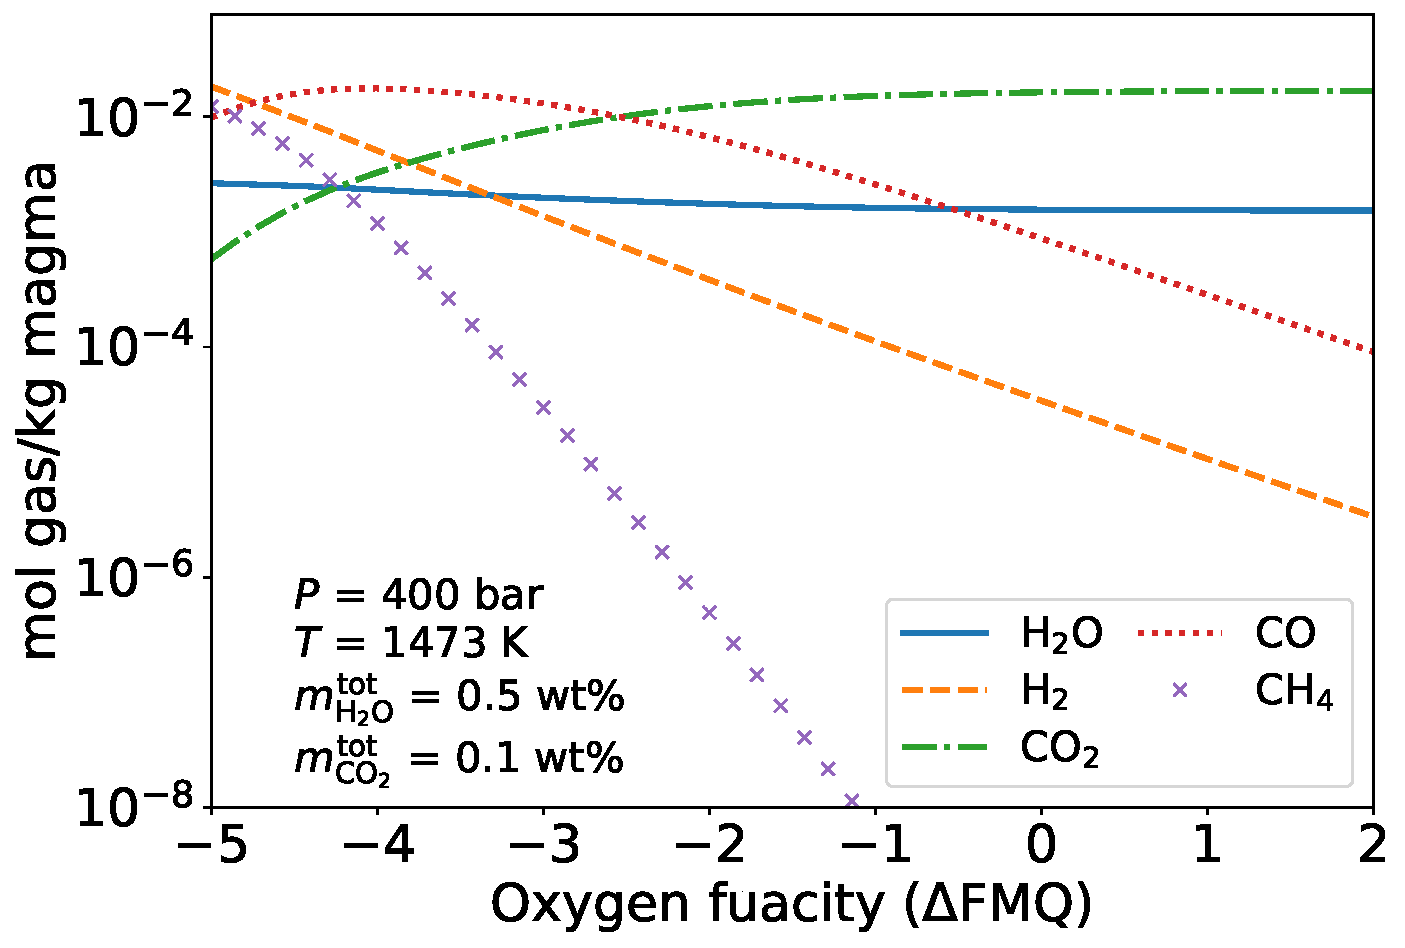
\includegraphics[width=10 cm]{tex/3methane/figures/fO2_dependence.pdf}
    \caption{Modeled volcanic outgassing speciation as a function of oxygen fugacity. Model assumes $P=400$ bar, $T=1473$ K, $m_\mathrm{H_2O}^\mathrm{tot}$ = 0.5 wt\%, and $m_\mathrm{CO_2}^\mathrm{tot}$ = 0.1 wt\%. Methane is most favorable at low oxygen fugacity.}
    \label{fig:fO2}
\end{figure}

\subsection{Carbon monoxide as a methane biosignature discriminant} \label{sec:CO_disc}

CO-consuming life evolved very early on Earth \citep{Adam_2018} and is a relatively simple metabolism. Therefore, it seems possible that life on other planets will evolve to consume CO. Planets with atmospheric CH$_4$+CO$_2$ produced by life might also have relatively small amounts of atmospheric CO because of CO consumers. Consequentially, the presence of abundant CO along with CH$_4$ can discriminate abiotic situations.

Monte-Carlo simulations shows that volcanoes should almost always produce more CO than CH$_4$ (Figure \ref{fig:result1}). Additionally, photochemical modeling (Figure \ref{fig:photosun} and \ref{fig:photoM}) suggests that CO should build up in the atmospheres of uninhabited planets with reducing submarine volcanic gases. Thus, atmospheric CO$_2$+CH$_4$ produced by volcanoes is likely accompanied by a large CO concentration. This is distinct from an inhabited world, which can have lower CO concentrations due to CO consuming life. 

However, the mere presence of large atmospheric CO is not a definitive sign of an uninhabited planet with reducing volcanic gases \citep{Schwieterman_2019}. This is because there are limits to how quickly gases can be transported from the atmosphere, into the ocean where they can be consumed by life \citep{Kharecha_2005}. For example, consider a planet with a very large volcanic CO flux (e.g., 100x modern). CO could build up in this planet's atmosphere even if CO consumers were present in an ocean because CO transport from the atmosphere to the ocean would not be sufficient to maintain low atmospheric CO. 

In summary, the CH$_4$+CO$_2$ biosignature is most compelling when the CO abundance is low or negligible because lack of CO potentially implies the presence of CO consuming biology. In comparison, atmospheric CH$_4$+CO$_2$ and large CO is ambiguous, and can either be explained by reducing volcanic gases or by an inhabited world that is unable to sequester atmospheric CO.

JWST might be able to put a tentative upper limit on atmospheric CO. \citet{Krissansen-Totton_2018a} simulated JWST retrievals of TRAPPIST-1e with an atmospheric composition similar to the Archean Earth containing 10 ppbv CO. Their synthetic retrieval suggested CO was below 652 ppmv with 90\% confidence after 10 transits. CO constraints could be improved by co-adding more transits and positive CO detections may also be possible with JWST \citep{Wunderlich_2020}.

However, even if observational CO constraints are poor, it may still be possible to say something about the abiotic or biotic origin of atmospheric CH$_4$. Reducing gases from volcanism are unlikely to mimic the modern biological CH$_4$ flux of 30 Tmol/yr (Section \ref{sec:littleCH4}). Additionally, serpentinization is unlikely to produce 30 Tmol CH$_4$/yr, and impact-generated CH$_4$ might be distinguished with system age \citep{Krissansen-Totton_2018b}. Therefore, JWST observations of atmospheric CH$_4$+CO$_2$ would be challenging to explain without the presence of biology regardless of atmospheric CO, as long as the CH$_4$ abundance implies a surface flux similar to the modern Earth's.

\subsection{CH$_4$ levels and implications for the origin on life}

Much current origin of life research revolves around the ``RNA world'' hypothesis \citep{Gilbert_1986,Joyce_2018,Sasselov_2020}. This hypothesis proposes an interval of time when primitive life consisted of self-replicating, evolving RNA molecules, which, at some point, were encapsulated in cells. On a rocky world, ``RNA world'' requires that RNA is synthesized from early raw materials. Laboratory experiments that have successfully synthesized nucleobases, which are building blocks of RNA, require the following nitriles: hydrogen cyanide (HCN), cyanoacetylene (HCCCN), and cyanogen (NCCN) \citep{Sutherland_2016,Ritson_2018,Benner_2019}. In addition, nitriles have also been used to synthesize amino acids \citep{Miller_1959,Sutherland_2016}.

The known natural source of nitriles is photochemistry in a chemically reducing atmosphere containing H$_2$, CH$_4$ and N$_2$ or perhaps NH$_3$. For example, Titan's photochemistry produces all the aforementioned nitriles \citep{Strobel_2009}. Importantly, to make the simplest nitrile, HCN, requires abundant CH$_4$ because HCN is formed from photochemical products of CH$_4$ and nitrogen \citep{Zahnle_1986,Tian_2011}.

Our results show that volcanic gases generally are unlikely to cause high atmospheric CH$_4$ abundances in prebiotic atmospheres. Consequently, the results lend credence to alternative proposals for making early CH$_4$-rich, reducing atmospheres, such as impacts \citep{Zahnle_2020}. Impacts can make a reducing atmosphere when reactions between iron-rich impact ejecta and shock-heated water vapor from an ocean generate copious H$_2$, CH$_4$ and NH$_3$. Subsequent photochemistry would generate HCN and other prebiotic nitriles over thousands to millions of years \citep{Zahnle_2020}.

\section{Conclusions}

Our modeling of volcanic outgassing speciation suggests that chemically reducing volcanism on terrestrial planets is unlikely to mimic biological CH$_4$ fluxes. The improbable cases where volcanoes do produce biological CH$_4$ fluxes also often produce CO. Volcanoes are not prone to produce CH$_4$ for several reasons. First, the high solubility of H$_2$O in magma limits the amount of total hydrogen outgassed, thus preventing the production of H-bearing molecules like CH$_4$. Second, CH$_4$ outgassing requires relatively low magma temperatures compared to the majority of magma erupted on Earth. Finally, CH$_4$ outgassing requires a very low magma oxygen fugacity unlike that of most terrestrial planets inferred from astronomical data \citep{Doyle_2019}.

We use a photochemical model to calculate atmospheric composition of planets with volcanoes that produce CH$_4$. We find that atmospheric CH$_4$ should coincide with abundant CO. On the other hand, biogenic CH$_4$ can coincide with a low CO abundance if CO-consuming microbial life is present.

Therefore, the CH$_4$-CO$_2$ biosignature is most compelling when little or no atmospheric CO is detected. Atmospheric CH$_4$-CO$_2$ and large CO is ambiguous and can be explained by an uninhabited planet with highly reducing volcanic gases, or an inhabited planet where biology is unable to sequester atmospheric CO \citep{Schwieterman_2019}.

However, observations of CO are not required to make conclusions about the abiotic or biotic origin of observed atmospheric CH$_4$. Atmospheric CH$_4$ and CO$_2$ alone would have a reasonable probability of being biological if the observed CH$_4$ abundance implies a surface flux similar to modern Earth’s biological CH$_4$ flux (30 Tmol/yr). Such a large CH$_4$ flux is difficult to explain with reducing volcanic gases or other abiotic processes that generate CH$_4$, such as serpentenization.

These conclusions should be taken with caution because they are based on what is understood about processes occurring on the Earth and our Solar System, which may be a very sparse sampling of what is possible.

\section{Chapter Appendix}

\subsection{Details of outgassing speciation model}

\subsubsection{Solubility constants for of H$_2$O and CO$_2$} \label{sec:solu_constants}
Our outgassing model uses solubility equations for H$_2$O and CO$_2$ in mafic magmas from \citet{Iacono-Marziano_2012} (Equations \eqref{eq:solu1} and \eqref{eq:solu2}). The parameters $S_1$ and $S_2$ in the solubility equations depend on the chemical make-up of the magma. We found that different mafic magma compositions did not significantly effect the outputs of our outgassing speciation model (Section \ref{sec:volcmodel}), therefore, for the purposes of calculating melt solubility, we fixed the chemical make-up of the magma to the magma erupting at Mt. Etna, Italy, reported by \citet{Iacono-Marziano_2012}. This reduced the complexity of the model without sacrificing any significant amount of accuracy.

Table \ref{tab:magmacomp} shows the chemical make-up of the magma at Mt. Etna, and Table \ref{tab:soluconst} shows several solubility constants from \citet{Iacono-Marziano_2012}. Together these values define the solubility parameters $S_1$ and $S_1$:
\begin{equation}
\begin{split}
    {S_1} &= \ln \left(\frac{\mu_\mathrm{magma}}{\mu_\mathrm{CO_2}10^{6}}\right) + \frac{{{C_{{\text{C}}{{\text{O}}_{\text{2}}}}}P}}{T} + {B_{{\text{C}}{{\text{O}}_{\text{2}}}}} + {b_{{\text{C}}{{\text{O}}_{\text{2}}}}}\left[ {\frac{{{\text{NBO}}}}{{\text{O}}}} \right] \\
    &+ \left( {\frac{{{x_{{\text{A}}{{\text{l}}_{\text{2}}}{{\text{O}}_{\text{3}}}}}}}{{{x_{{\text{CaO}}}} + {x_{{{\text{K}}_{\text{2}}}{\text{O}}}} + {x_{{\text{N}}{{\text{a}}_{\text{2}}}{\text{O}}}}}}} \right){d_{{\text{A}}{{\text{l}}_{\text{2}}}{{\text{O}}_{\text{3}}}{\text{/(CaO + }}{{\text{K}}_{\text{2}}}{\text{O + N}}{{\text{a}}_{\text{2}}}{\text{O)}}}}\\
    &+ ({x_{{\text{FeO}}}} + {x_{{\text{MgO}}}}){d_{{\text{FeO + MgO}}}} + ({x_{{\text{N}}{{\text{a}}_{\text{2}}}{\text{O}}}} + {x_{{{\text{K}}_{\text{2}}}{\text{O}}}}){d_{{\text{N}}{{\text{a}}_2}{\text{O + }}{{\text{K}}_2}{\text{O}}}}
\end{split}
\end{equation}
\begin{equation}
    {S_2} = \ln \left(\frac{\mu_\mathrm{magma}}{{\mu_{{{\text{H}}_2}{\text{O}}}}10^2}\right) + \frac{{{C_{{{\text{H}}_2}{\text{O}}}}P}}{T} + {B_{{{\text{H}}_2}{\text{O}}}} + {b_{{{\text{H}}_2}{\text{O}}}}\left[ {\frac{{{\text{NBO}}}}{{\text{O}}}} \right]
\end{equation}
\begin{equation}
    \left[ {\frac{{{\text{NBO}}}}{{\text{O}}}} \right] = \frac{{2({x_{{{\text{K}}_{\text{2}}}{\text{O}}}} + {x_{{\text{N}}{{\text{a}}_{\text{2}}}{\text{O}}}} + {x_{{\text{CaO}}}} + {x_{{\text{MgO}}}} + {x_{{\text{FeO}}}} - {x_{{\text{A}}{{\text{l}}_{\text{2}}}{{\text{O}}_{\text{3}}}}})}}{{2{x_{{\text{Si}}{{\text{O}}_{\text{2}}}}} + 2{x_{{\text{Ti}}{{\text{O}}_{\text{2}}}}} + 3{x_{{\text{A}}{{\text{l}}_{\text{2}}}{{\text{O}}_{\text{3}}}}} + {x_{{\text{MgO}}}} + {x_{{\text{FeO}}}} + {x_{{\text{CaO}}}} + {x_{{\text{N}}{{\text{a}}_{\text{2}}}{\text{O}}}} + {x_{{{\text{K}}_{\text{2}}}{\text{O}}}}}}
\end{equation}
Here, $T$ is magma temperature, $P$ is the total pressure of degassing, and $\left[\frac{\mathrm{NBO}}{\mathrm{O}}\right]$ is the amount of non-bridging oxygen per oxygen in the melt.

\begin{table}[]
  \caption{Mt. Etna magma composition}
  \label{tab:magmacomp}
  \centering
  \begin{tabular}{l c}
  \hline \hline
  Magma component & Mole fraction \\
  \hline
  $x_\mathrm{SiO_2}$     & 0.516   \\
  $x_\mathrm{TiO_2}$     & 0.014   \\
  $x_\mathrm{Al_2O_3}$     & 0.110   \\
  $x_\mathrm{FeO}$     & 0.091   \\
  $x_\mathrm{MgO}$     & 0.092   \\
  $x_\mathrm{CaO}$     & 0.126   \\
  $x_\mathrm{Na2O}$     & 0.035   \\
  $x_\mathrm{K_2O}$     & 0.002   \\
  $x_\mathrm{P_2O_5}$     & 0.016   \\
  \hline
  \multicolumn{2}{l}{Note. Taken from \citet{Iacono-Marziano_2012}.} 
  \end{tabular}
\end{table}

\begin{table}
  \caption{Solubility constants}
  \label{tab:soluconst}
  \centering
  \begin{tabular}{l c}
  \hline \hline
  Constant & Value \\
  \hline
  $C_\mathrm{CO_2}$     & 0.14   \\
  $B_\mathrm{CO_2}$     & -5.3   \\
  $b_\mathrm{CO_2}$     & 15.8   \\
  $B_\mathrm{H_2O}$     & -2.95   \\
  $b_\mathrm{H_2O}$     & 1.24   \\
  $d_\mathrm{Al_2O_3/(CaO+K_2O+Na_2O)}$     & 3.8   \\
  $d_\mathrm{FeO+MgO}$     & -16.3   \\
  $d_\mathrm{Na_2O+K_2O}$     & 20.1   \\
  \hline
  \multicolumn{2}{l}{Note. ``Anhydrous'' case from \citet{Iacono-Marziano_2012}.} 
  \end{tabular}
\end{table}

\subsubsection{Derivation of Equations \eqref{eq:C_con} and \eqref{eq:H_con}} \label{sec:Derivation_con}

Following is the derivation for the atom conservation equation for carbon used in our outgassing model (Equation \eqref{eq:C_con}). The derivation for the atom conservation equation for hydrogen follows the exact same procedure, so we do not include it. 

Consider some volume of magma with gas bubbles in it which contains a total number of moles $\gamma_\mathrm{tot}$. The total moles is the sum of the moles of magma ($\gamma_\mathrm{magma}$), and the moles of gas in bubbles suspended in that magma ($\gamma_\mathrm{gas}$):
\begin{equation} \label{eq:tot_con}
    \gamma_\mathrm{tot} = \gamma_\mathrm{gas} + \gamma_\mathrm{magma}
\end{equation}
Within this same volume of magma, the total moles of carbon ($\gamma_\mathrm{C}^\mathrm{tot}$) is equal to the moles of carbon in the gas phase ($\gamma_\mathrm{C}^\mathrm{gas}$) and the moles of carbon dissolved in the magma ($\gamma_\mathrm{C}^\mathrm{magma}$) combined. 
\begin{equation} \label{eq:CO2_con}
    \gamma_\mathrm{C}^\mathrm{tot} = \gamma_\mathrm{C}^\mathrm{gas} + \gamma_\mathrm{C}^\mathrm{magma}
\end{equation}
We assume that the only carbon bearing molecule that can dissolve in the magma is CO$_2$, therefore $\gamma_\mathrm{C}^\mathrm{magma}=\gamma_\mathrm{CO_2}^\mathrm{magma}$. Dividing by $\gamma_\mathrm{tot}$ and expanding gives
\begin{equation} 
    \frac{\gamma_\mathrm{C}^\mathrm{tot}}{\gamma_\mathrm{tot}} = \frac{\gamma_\mathrm{gas}}{\gamma_\mathrm{tot}}\frac{\gamma_\mathrm{C}^\mathrm{gas}}{\gamma_\mathrm{gas}} + \frac{\gamma_\mathrm{magma}}{\gamma_\mathrm{tot}}\frac{\gamma_\mathrm{CO_2}^\mathrm{magma}}{\gamma_\mathrm{magma}}
\end{equation}
We can replace $\frac{\gamma_\mathrm{magma}}{\gamma_\mathrm{tot}}$ with $1-\frac{\gamma_\mathrm{gas}}{\gamma_\mathrm{tot}}$ using Equation \eqref{eq:tot_con}. This leaves us with
\begin{equation} 
    \frac{\gamma_\mathrm{C}^\mathrm{tot}}{\gamma_\mathrm{tot}} = \frac{\gamma_\mathrm{gas}}{\gamma_\mathrm{tot}}\frac{\gamma_\mathrm{C}^\mathrm{gas}}{\gamma_\mathrm{gas}} + \left(1-\frac{\gamma_\mathrm{gas}}{\gamma_\mathrm{tot}}\right)\frac{\gamma_\mathrm{CO_2}^\mathrm{magma}}{\gamma_\mathrm{magma}}
\end{equation}
Here, $\frac{\gamma_\mathrm{CO_2}^\mathrm{magma}}{\gamma_\mathrm{magma}}$ is just $x_\mathrm{CO_2}$ (the mol fraction of CO$_2$ in the magma, see Table \ref{tab:1}). Also, we assume that CO$_2$, CO and CH$_4$ are the only carbon-bearing gas species, so $\gamma_\mathrm{C}^\mathrm{gas}=\gamma_\mathrm{CO_2}^\mathrm{gas}+\gamma_\mathrm{CO}^\mathrm{gas}+\gamma_\mathrm{CH_4}^\mathrm{gas}$. Making substitutions gives
\begin{equation} 
    \frac{\gamma_\mathrm{C}^\mathrm{tot}}{\gamma_\mathrm{tot}} = \frac{\gamma_\mathrm{gas}}{\gamma_\mathrm{tot}}\frac{\gamma_\mathrm{CO_2}^\mathrm{gas}+\gamma_\mathrm{CO}^\mathrm{gas}+\gamma_\mathrm{CH_4}^\mathrm{gas}}{\gamma_\mathrm{gas}} + \left(1-\frac{\gamma_\mathrm{gas}}{\gamma_\mathrm{tot}}\right)x_\mathrm{CO_2}
\end{equation}
Assuming the ideal gas law, $\gamma_i^\mathrm{gas}/\gamma_\mathrm{gas}=P_i/P$. Also, to make the equation more manageable, we substitute $\alpha_\mathrm{gas}=\frac{\gamma_\mathrm{gas}}{\gamma_\mathrm{tot}}$, which is the total mols in the gas phase divided by the moles in the gas phase and magma combined.
\begin{equation} \label{eq:IDK}
    \frac{\gamma_\mathrm{C}^\mathrm{tot}}{\gamma_\mathrm{tot}} = \frac{P_\mathrm{CO_2}+P_\mathrm{CO}+P_\mathrm{CH_4}}{P}\alpha_\mathrm{gas} + \left(1-\alpha_\mathrm{gas}\right)x_\mathrm{CO_2}
\end{equation}
Magma sometimes freezes deep in the Earth as a glass before it releases any volatiles. Measurements of volatiles like CO$_2$, in such glasses are reported in terms of mass fractions \citep{Wallace_2015}. To stay consistent with these unit conventions, we indicate the total carbon in undegassed magma as a mass fraction of CO$_2$ ($m_\mathrm{CO2}^\mathrm{tot}$). We can convert the mass fraction to a mole fraction using Equation \eqref{eq:convert}:
\begin{equation} \label{eq:IDK2}
    \frac{m_\mathrm{CO2}^\mathrm{tot}\mu_\mathrm{magma}}{\mu_\mathrm{CO_2}}=x_\mathrm{CO2}^\mathrm{tot}=\frac{\gamma_\mathrm{CO_2}^\mathrm{tot}}{\gamma_\mathrm{tot}}=\frac{\gamma_\mathrm{C}^\mathrm{tot}}{\gamma_\mathrm{tot}}
\end{equation}
Substituting Equation \eqref{eq:IDK2} into Equation \eqref{eq:IDK} gives 
\begin{equation} \label{eq:LAST}
    {\frac{{m_{{\text{C}}{{\text{O}}_{\text{2}}}}^{{\text{tot}}}}\mu_\mathrm{magma}}{{{\mu_{{\text{C}}{{\text{O}}_{\text{2}}}}}}}} = \frac{{{P_{{\text{C}}{{\text{O}}_{\text{2}}}}} + {P_{{\text{CO}}}} + {P_{{\text{C}}{{\text{H}}_{\text{4}}}}}}}{P}{\alpha _{{\text{gas}}}} + (1 - {\alpha _{{\text{gas}}}}){x_{{\text{C}}{{\text{O}}_{\text{2}}}}}
\end{equation}
Equation \eqref{eq:LAST} is identical to Equation \eqref{eq:C_con}.

\subsubsection{Graphite saturation and the solubility of CO, CH$_4$, and H$_2$} \label{sec:graphite_sat}

Several studies have shown that degassing can be affected by graphite saturation of of magma \citep{Hirschmann_2008} or by the solubility of CO, CH$_4$, and H$_2$ in magma \citep{Wetzel_2013,Ardia_2013,Hirschmann_2012}. Our model for outgassing speciation used throughout the main text does not account for these complications. Here, we show that our assumption is valid because it does not significantly change our results.

Consider the following equilibrium.
\begin{equation}
    \mathrm{C}+\mathrm{O_2}\leftrightarrow\mathrm{CO_2}
\end{equation}
\begin{equation} \label{eq:graphite_sat}
    K_9=\frac{f_\mathrm{CO_2}}{a_\mathrm{C}f_\mathrm{O_2}}\approx \frac{P_\mathrm{CO_2}}{a_\mathrm{C}f_\mathrm{O_2}}
\end{equation}
Here, $K_9$ is the equilibrium constant given by $\exp(47457/T+0.136)$, and $a_\mathrm{C}$ is the activity of carbon. To incorporate graphite saturation into our model, we first calculate outgassing speciation using the model described in the main text (Section \ref{sec:volcmodel}). Next, we check for graphite saturate by calculating the activity of carbon using Equation \eqref{eq:graphite_sat}. If $a_\mathrm{C}<1$, then we assume the melt is not graphite saturated and that the calculation is valid. If $a_\mathrm{C}>1$, then we assume graphite is saturated and recalculate outgassing speciation by replacing the carbon conservation equation (Equation \eqref{eq:C_con}), with the graphite saturation equation  with $a_\mathrm{C}=1$ (Equations \eqref{eq:graphite_sat}). Here, we are considering graphite saturation in the magma just before degassing occurs. Our treatment is different than, for example, the methods of \citet{Ortenzi_2020} because they are accounting for graphite saturation much deeper in a planet during partial melting of the mantle.

Figure \ref{fig:graphite} is identical to Figure \ref{fig:result1}, except Figure \ref{fig:graphite} accounts for graphite saturation. Graphite saturation appears to have a small effect on the results, therefore it is justified to ignore it.

\begin{figure}
    \centering
    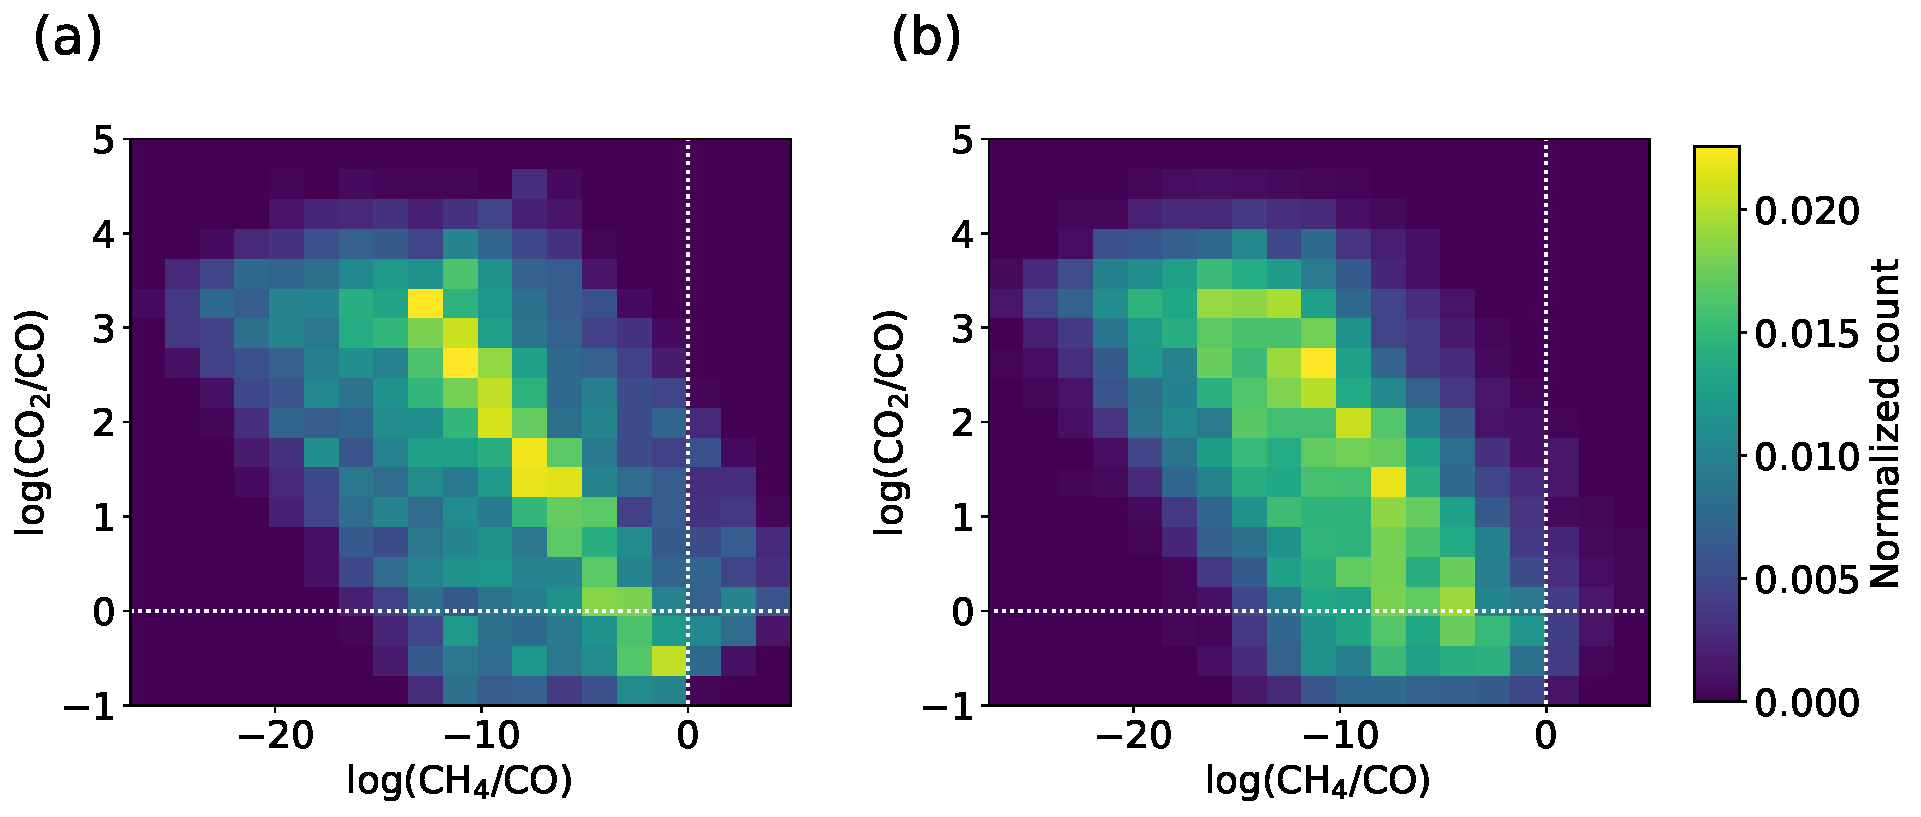
\includegraphics[width=\textwidth]{tex/3methane/figures/both_Csat.pdf}
    \caption{Identical to Figure \ref{fig:result1}, except here we account for graphite saturation in the melt. Like Figure \ref{fig:result1} (a) is for ocean worlds and (b) is for Earth-like worlds. Graphite saturation has a small effect on the results.}
    \label{fig:graphite}
\end{figure}

To incorporate the solubility of H$_2$, CH$_4$, and CO into our model, we add the following solubility relationships to or system of original outgassing equations (Section \ref{sec:volcmodel}).
\begin{equation}
    \exp(-11.403-0.000076P)=K_5=\frac{x_\mathrm{H_2}}{f_\mathrm{H_2}} \approx \frac{x_\mathrm{H_2}}{P_\mathrm{H_2}}
\end{equation}
\begin{equation}
    \exp(-7.63-0.000193P)=K_6=\frac{x_\mathrm{CH_4}}{f_\mathrm{CH_4}} \approx \frac{x_\mathrm{CH_4}}{P_\mathrm{CH_4}}
\end{equation}
\begin{equation} \label{eq:COsolub}
    \exp(-41.02-0.00056P) = K_7 = \frac{x_\mathrm{Fe(CO)_5}}{a_\mathrm{Fe}f_\mathrm{CO}^5} \approx \frac{x_\mathrm{Fe(CO)_5}}{a_\mathrm{Fe}P_\mathrm{CO}^5}
\end{equation}
Here, pressure dependent equilibrium constants $K_5$, $K_6$ and $K_7$ are from \citet{Hirschmann_2012}, \citet{Ardia_2013}, and \citet{Wetzel_2013}, respectively. For Equation \eqref{eq:COsolub}, we take the activity of iron to be $a_\mathrm{Fe}=0.6$ based on the experiments in \citet{Wetzel_2013}. Also, we only include the Equation \eqref{eq:COsolub} when the $f_\mathrm{O_2}<$ IW-0.55 (IW is the Iron-Wustite mineral buffer) because \citet{Wetzel_2013} only observed CO dissolved in magma for these low oxygen fugacities.

We also alter the carbon and hydrogen atom conservation equations to accommodate for new molecules in the melt.
\begin{equation} 
    \frac{m_\mathrm{CO_2}^\mathrm{tot}\mu_\mathrm{magma}}{\mu_\mathrm{CO_2}} = \frac{P_\mathrm{CO_2}+P_\mathrm{CO}+P_\mathrm{CH_4}}{P}\alpha_\mathrm{gas} + \left(1-\alpha_\mathrm{gas}\right)(x_\mathrm{CO_2}+x_\mathrm{CO}+x_\mathrm{CH_4})
\end{equation}
\begin{equation} 
    \frac{m_\mathrm{H_2O}^\mathrm{tot}\mu_\mathrm{magma}}{\mu_\mathrm{H_2O}} = \frac{P_\mathrm{H_2O}+P_\mathrm{H_2}+2P_\mathrm{CH_4}}{P}\alpha_\mathrm{gas} + \left(1-\alpha_\mathrm{gas}\right)(x_\mathrm{H_2O}+x_\mathrm{H_2}+2x_\mathrm{CH_4})
\end{equation}
Here, $x_i$ is the mol fraction of species $i$ in the melt.

Figure \ref{fig:Ch4COH2solu} is identical to Figure \ref{fig:result1}, except Figure \ref{fig:Ch4COH2solu} accounts for H$_2$, CH$_4$ and CO solubility in magma. The solubility of these three molecules has a small effect on the results, therefore they can be ignored.

\begin{figure}
    \centering
    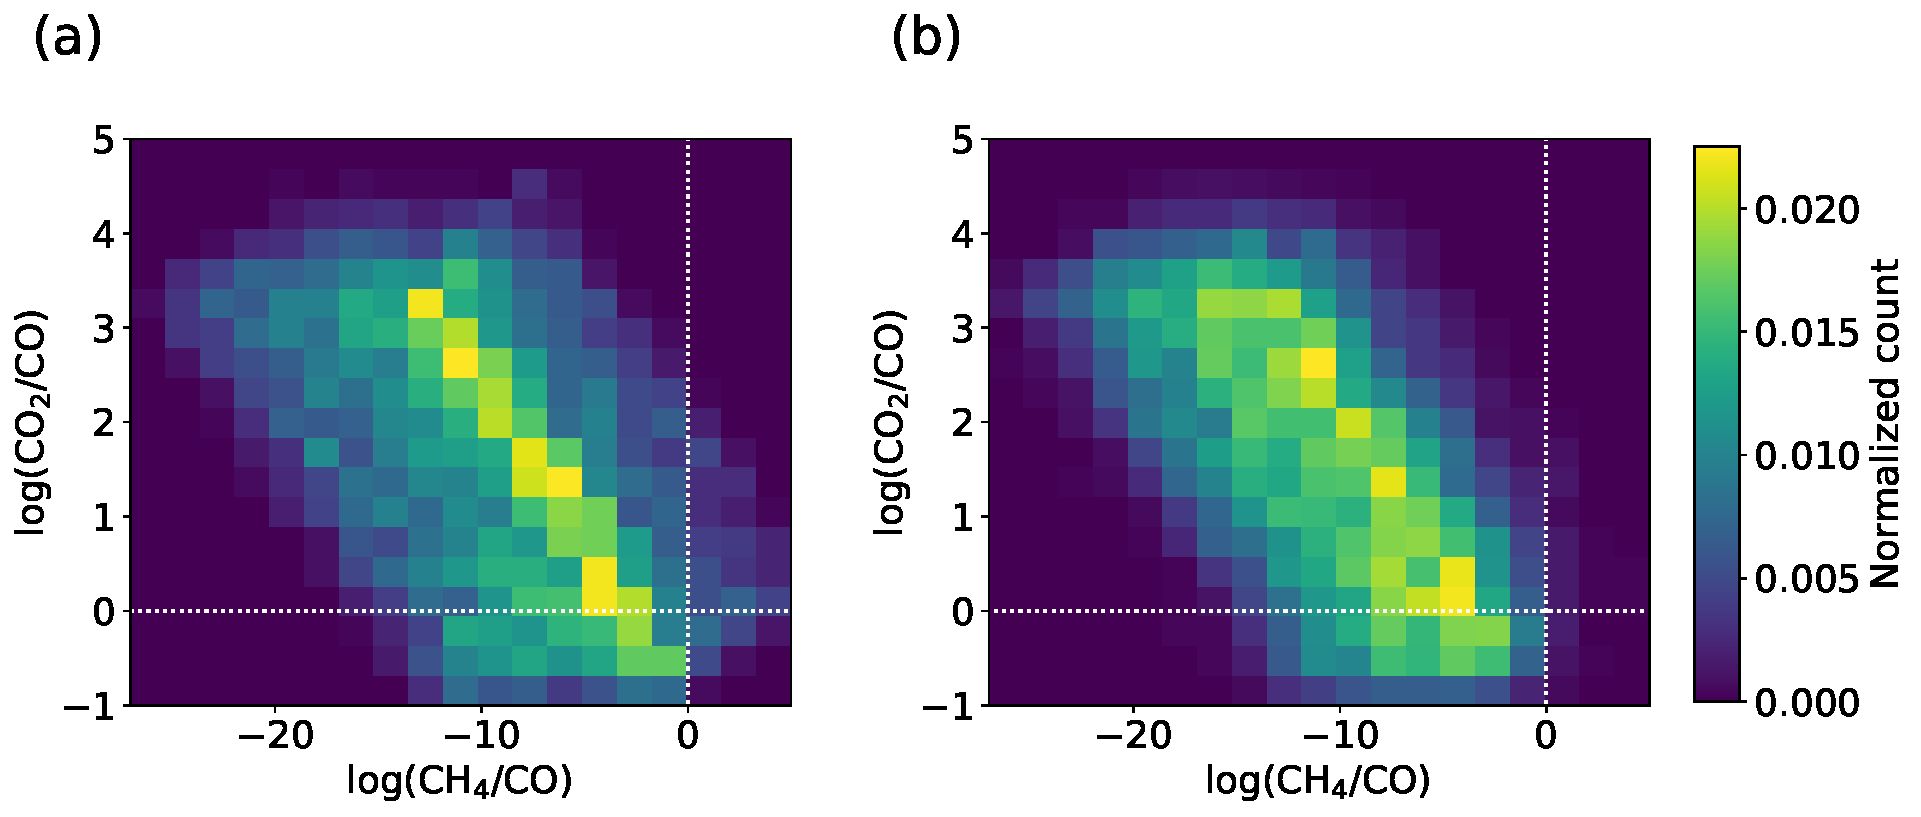
\includegraphics[width=\textwidth]{tex/3methane/figures/both_CO_H2_CH4_solu.pdf}
    \caption{Identical to Figure \ref{fig:result1}, except here we account for the solubility of H$_2$, CH$_4$ and CO in the melt. Like Figure \ref{fig:result1} (a) is for ocean worlds and (b) is for Earth-like worlds. H$_2$, CH$_4$ and CO  solubility has a small effect on the results.}
    \label{fig:Ch4COH2solu}
\end{figure}

\subsubsection{Closed system cooling and chemical kinetics}\label{sec:kinetics}

Our model for volcanic outgassing is a thermodynamic equilibrium model. We assume that during magma eruptions gas bubbles chemically and thermally equilibrate with magma, and then are released to the atmosphere unaltered (Figure \ref{fig:imagine}). This does not exactly reflect real degassing. 

In reality, the chemical composition of gas bubbles changes as bubbles leave the magma and enter the atmosphere \citep{Moussallam_2019, Kadoya_2020}. As a bubble leaves magma, it cools down, and new chemical equilibria are preferred. When the gas bubble first begins cooling, it is still very hot, so chemical reactions keep the bubble near chemical equilibrium. Once the bubble is cold enough, chemical reactions slow, and ultimately cease, quenching or freezing the chemical composition of the gas bubble. Therefore, the cooling process alters the chemistry of the gas. 

Gas re-equilibration to lower temperatures explains the observed chemistry of volcanic gases globally \citep{Moussallam_2019}, and \citet{Oppenheimer_2018} provides a specific example of this phenomenon at Kilauea volcano, Hawaii. During eruptions at Kilauea, gas bubbles in the magma would rise to the surface. As the bubbles rose in the magma, they adiabatically expanded, which cooled the gas below the temperature of the magma. Chemical reactions during adiabatic expansion changed the chemical make-up of the bubble.

For the purposes of understanding potential CH$_4$ biosignature false positives from volcanoes, we need to know if bubble cooling might generate a substantial amount of CH$_4$. Here, we first consider the kinetics of methane generation and show that reactions are likely too slow to generate substantial CH$_4$ during gas cooling. Next, we show that our Monte Carlo simulation results (Figure \ref{fig:CH4}) remain qualitatively unchanged even if our kinetics calculations are wrong, and CH$_4$ can be generated during gas cooling.

CO or CO$_2$ is converted to CH$_4$ through either of the net reactions \citep{Schaefer_2010}
\begin{equation}
    \mathrm{CO}+3\mathrm{H_2} \leftrightarrow \mathrm{CH_4} + \mathrm{H_2O}
\end{equation}
\begin{equation}
    \mathrm{CO_2}+4\mathrm{H_2} \leftrightarrow \mathrm{CH_4} + \mathrm{2H_2O}
\end{equation}
The rate limiting step to either CO or CO$_2$ conversion to CH$_4$ is debated in the literature \citep{Zahnle_2014}, but following are two good candidates and their corresponding rate constants:
\begin{equation}
    \mathrm{H_2}+\mathrm{H_2CO} \rightarrow \mathrm{CH_3} + \mathrm{OH}
\end{equation}
\begin{equation}
    k_{10} = 2.3\times10^{-10}\exp(-36200/T)
\end{equation}
\begin{equation}
    \mathrm{H}+\mathrm{H_2CO} \rightarrow \mathrm{CH_3} 
\end{equation}
\begin{equation}
    k_{12} = 4.0\times10^{-11}\exp(-2068/T)
\end{equation}
Here, $k_{10}$ and $k_{12}$ are rate constants (cm$^3$ s$^{-1}$). The lifetime of CO or CO$_2$ conversion to CH$_4$ is thus one of the following
\begin{equation} \label{eq:first_time}
    \tau_{10}(\mathrm{CO})=\frac{N_\mathrm{CO}}{k_{10}N_\mathrm{H_2}N_\mathrm{H_2CO}}
\end{equation}
\begin{equation}
    \tau_{12}(\mathrm{CO})=\frac{N_\mathrm{CO}}{k_{12}N_\mathrm{H}N_\mathrm{H_2CO}}
\end{equation}
\begin{equation}
    \tau_{10}(\mathrm{CO_2})=\frac{N_\mathrm{CO_2}}{k_{10}N_\mathrm{H_2}N_\mathrm{H_2CO}}
\end{equation}
\begin{equation} \label{eq:last_time}
    \tau_{12}(\mathrm{CO_2})=\frac{N_\mathrm{CO_2}}{k_{12}N_\mathrm{H}N_\mathrm{H_2CO}}
\end{equation}
Here, $\tau$ is chemical lifetime in seconds, and $N_i$ is number density of species $i$ in molecules cm$^{-3}$.

Figure \ref{fig:kinetics} shows timescales of CH$_4$ generation (Equations \eqref{eq:first_time}-\eqref{eq:last_time}) during the closed system cooling of submarine volcanic gas. To determine gas chemistry just before a bubble is released from magma we use our speciation model (section \ref{sec:volcmodel}). At 1473 K we calculate gas speciation assuming $P =$ 400 bar, $f_\mathrm{O_2} =$ FMQ-4, $m_\mathrm{CO_2}^{\mathrm{tot}} =$ 0.1\%, $m_\mathrm{H_2O}^{\mathrm{tot}} =$ 0.5\%.  We then calculate new chemical equilibrium as the gas cools assuming it is a closed system, i.e. we assume the gas is thermally and chemically decoupled from the magma (Figure \ref{fig:kinetics}a). Figure \ref{fig:kinetics}b shows the corresponding timescale of CH$_4$ generation (Equations \eqref{eq:first_time}-\eqref{eq:last_time}) at each temperature.

The “quench” temperature, i.e. the temperature where outgassing chemistry is frozen-in due to slow kinetics, of CH$_4$ depends on the cooling timescale of volcanic gases (not shown in Figure \ref{fig:kinetics}). CH$_4$ should quench where the cooling timescale is about the same as the timescale of CH$_4$ generation. After gases are released from a submarine volcano, we suspect they cool from magma temperatures to ocean temperatures on the order of seconds. If this is the case, then the CH$_4$ quench temperature is probably $>$1400 K. This would result in a negligible increase in the CH$_4$ content of the gas (Figure \ref{fig:kinetics}a).

\begin{figure}
    \centering
    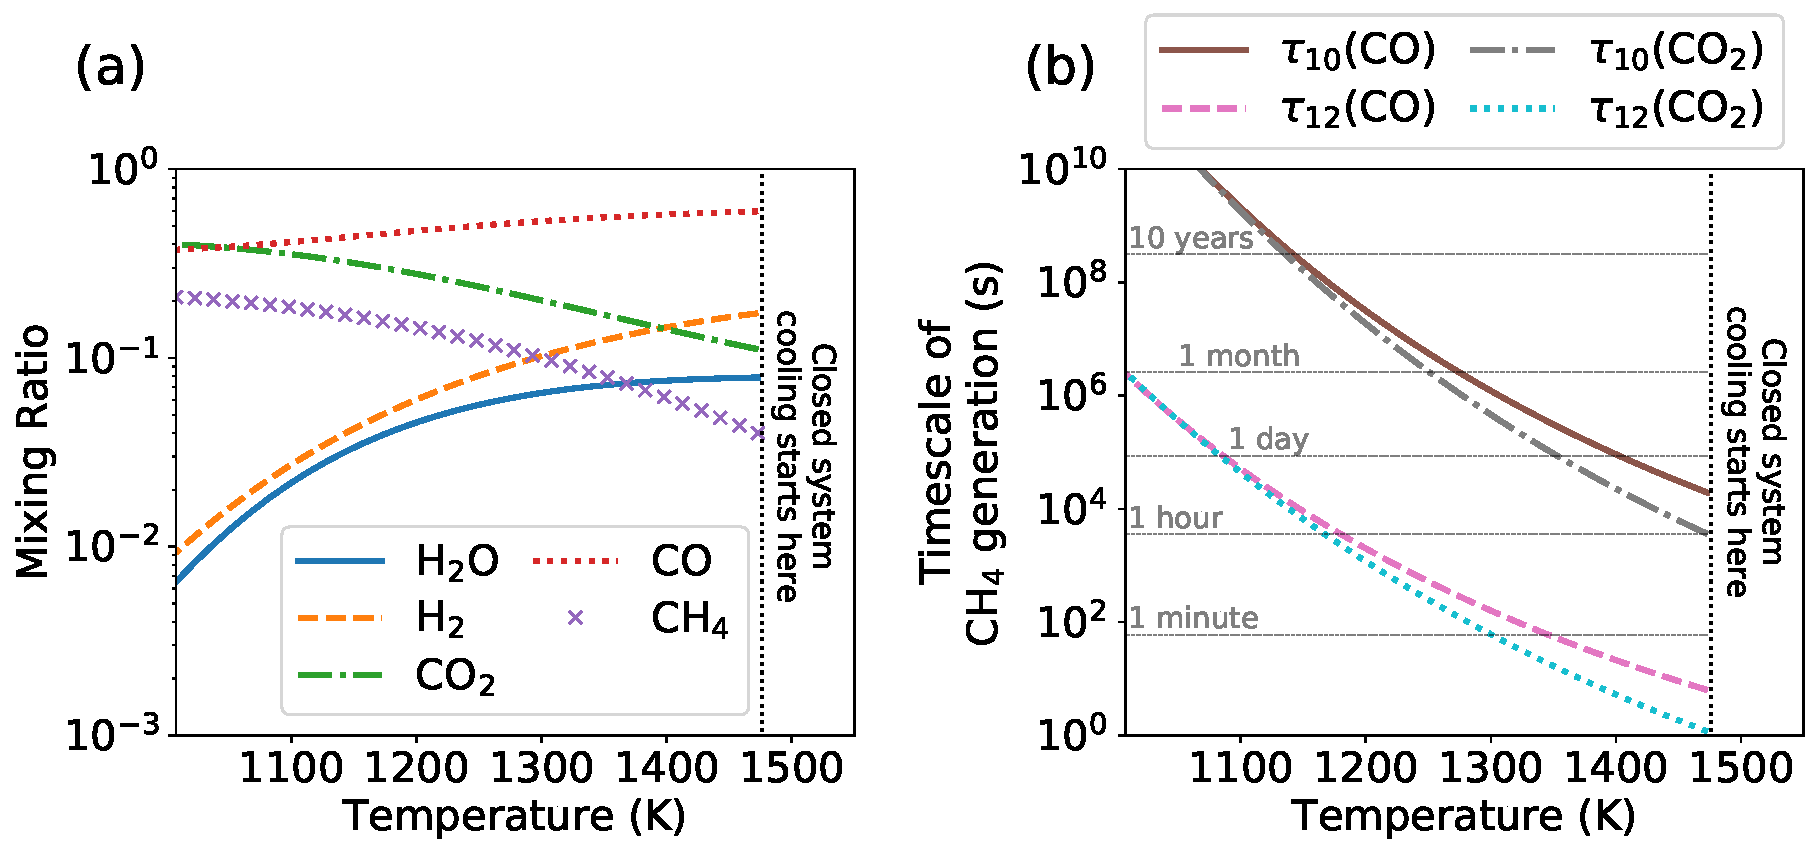
\includegraphics[width=\textwidth]{tex/3methane/figures/kinetics.pdf}
    \caption{(a) Equilibrium composition as a function of temperature for a submarine volcanic gas which is cooled as a closed system and (b) timescales of CH$_4$ formation during closed system cooling. Timescales of volcanic gas cooling are not shown or calculated.}
    \label{fig:kinetics}
\end{figure}

\begin{table}[hbt!]
  \caption{Boundary conditions for photochemical modeling}
  \label{tab:photochem_model}
  \centering
  \begin{tabularx}{\textwidth}{l c c c}
  \hline \hline
  Chemical Species & Deposition Velocity (cm s$^{-1}$) & Mixing Ratio & Flux (molecules cm$^{-2}$ s$^{-1}$)   \\
  \hline
  $\mathrm{O}$ & 1 & ... & ... \\
  $\mathrm{O_2}$ & $1.4\times10^{-4}$ & ... & ... \\
  $\mathrm{H_2O}$ & 0 & ... & ... \\
  $\mathrm{H}$ & 1 & ... & ... \\
  $\mathrm{OH}$ & 1 & ... & ... \\
  $\mathrm{HO_2}$ & 1 & ... & ... \\
  $\mathrm{H_2O_2}$ & $2\times10^{-1}$ & ... & ... \\
  $\mathrm{H_2}$ & 0 & ... & $5.9F_\mathrm{CH_4}$ \\
  $\mathrm{CO}$ & $1\times10^{-8}$ & ... & $1.7F_\mathrm{CH_4}$ \\
  $\mathrm{HCO}$ & 1 & ... & ... \\
  $\mathrm{H_2CO}$ & $2\times10^{-1}$ & ... & ... \\
  $\mathrm{CH_4}$ & 0 & ... & variable \\
  $\mathrm{CH_3}$ & 1 & ... & ... \\
  $\mathrm{C_2H_6}$ & 0 & ... & ... \\
  $\mathrm{NO}$ & $3\times10^{-4}$ & ... & ... \\
  $\mathrm{NO_2}$ & $3\times10^{-3}$ & ... & ... \\
  $\mathrm{HNO}$ & 1 & ... & ... \\
  $\mathrm{O_3}$ & $7\times10^{-2}$ & ... & ... \\
  $\mathrm{HNO_3}$ & $2\times10^{-1}$ & ... & ... \\
  $\mathrm{H_2S}$ & $2\times10^{-2}$ & ... & $0.1F_\mathrm{CH_4}$ \\
  $\mathrm{SO_3}$ & 0 & ... & ... \\
  $\mathrm{S_2}$ & 0 & ... & ... \\
  $\mathrm{HSO}$ & 1 & ... & ... \\
  $\mathrm{H_2SO_4}$ & 1 & ... & ... \\
  $\mathrm{SO_2}$ & 1 & ... & $0.1F_\mathrm{CH_4}$ \\
  $\mathrm{SO}$ & 0 & ... & ... \\
  $\mathrm{SO_4}$ aerosol & $1\times10^{-2}$ & ... & ... \\
  $\mathrm{S_8}$ aerosol & $1\times10^{-2}$ & ... & ... \\
  hydrocarbon aerosol & $1\times10^{-2}$ & ... & ... \\
  $\mathrm{CO_2}$ & ... & variable & ... \\
  $\mathrm{N_2}$ & ... & 0.8 & ... \\
  \hline
  \multicolumn{4}{>{\raggedright\arraybackslash}p{\textwidth}}{Notes. Species included in the photochemical scheme with a deposition velocity and flux of 0 include N, $\mathrm{C_3H_2}$, C$_3$H$_3$, CH$_3$C$_2$H, CH$_2$CCH$_2$, C$_3$H$_5$, C$_2$H$_5$CHO, C$_3$H$_6$, C$_3$H$_7$, C$_3$H$_8$, C$_2$H$_4$OH, C$_2$H$_2$OH, C$_2$H$_5$, C$_2$H$_4$, CH, CH$_3$O$_2$, CH$_3$O, CH$_2$CO, CH$_3$CO, CH$_3$CHO, C$_2$H$_2$, (CH$_2$)$_3$, C$_2$H, C$_2$, C$_2$H$_3$, HCS, CS$_2$, CS, OCS, S, and HS. Here, deposition velocities follow those used by \citet{Schwieterman_2019}.} 
  \end{tabularx}
\end{table}

Suppose that the CH$_4$ quench temperature was instead 1000 K. In this case, the CH$_4$ content of the gas would be increased by about a factor of 5 (Figure \ref{fig:kinetics}a). There are two ways that a $\sim$1000 K CH$_4$ quench is possible. First, gas cooling could occur on timescales of months rather than seconds. According to Figure \ref{fig:kinetics}b, month-long gas cooling should quench CH$_4$ by 1000 K. Second, catalysts could dramatically speed up the reactions creating CH$_4$, which might allow for quench temperatures near 1000 K for even gas cooling timescales of seconds. In the following two paragraphs we show that either of these scenario would not significantly change our results. 

To demonstrate that re-equilibration of gases to feasible lower temperatures does not change our conclusions, assuming low CH$_4$ quench temperatures can be achieved, we perform another Monte-Carlo simulation identical to the one described in Section \ref{sec:monte} except we account for closed system cooling of volcanic gases. In the Monte-Carlo simulation we first calculate gas composition using our outgassing model (Section \ref{sec:volcmodel}), then we re-equilibrate this gas mixture to the uniformly sampled gas equilibrium temperature between 800 and 1500 K. This range of gas equilibrium temperatures is the range observed in Earth's volcanic gases \citep{Moussallam_2019}. In cases where the randomly drawn gas equilibrium temperature is higher than the magma temperature, we assume no closed system cooling occurs.

Figure \ref{fig:CH4_closed} is identical to Figure \ref{fig:CH4}c and \ref{fig:CH4}d, except Figure \ref{fig:CH4_closed} accounts for closed system cooling of gases. Closed system cooling allows more CH$_4$ production on average, but still only 0.3\% and 0.1\% of calculations for ocean worlds or earth-like worlds respectively produce more than 10 Tmol CH$_4$/yr. The probability of volcanic CH$_4$ fluxes being comparable to modern Earth's biological flux (30 Tmol/yr) is still low.

\begin{figure*}
    \centering
    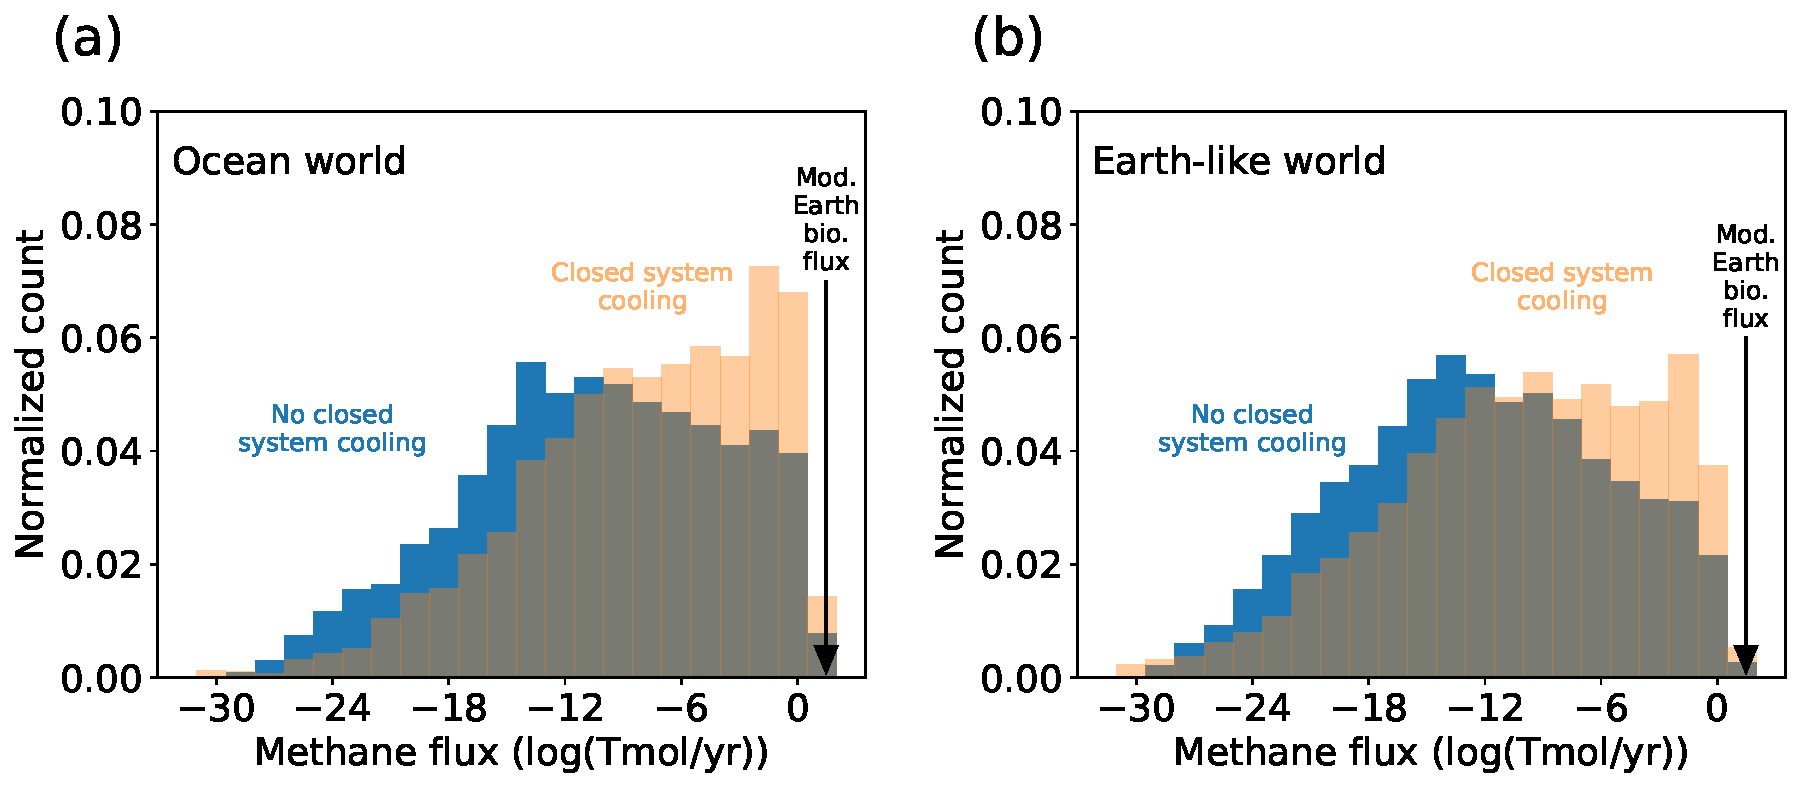
\includegraphics[width=\textwidth]{tex/3methane/figures/CH4_prod_closedsystem.pdf}
    \caption{The blue histograms in (a) and (b) are identical to Figure \ref{fig:CH4}c and \ref{fig:CH4}d, and orange histograms are identical Monte Carlo simulations except they account for the closed system cooling of volcanic gases to equilibrium temperatures observed on Earth (800 to 1500 K). To calculate CH$_4$ fluxes, we used modern Earth's magma production rate.}
    \label{fig:CH4_closed}
\end{figure*}

In summary, changes in gas chemistry during cooling might cause our speciation model to under-predict the CH$_4$ produced by an amount that does not change our conclusions significantly. Further consideration of the kinetics of CH$_4$ generation in volcanic gases is beyond the scope of this paper.

\subsection{Photochemical model boundary conditions} \label{sec:photo_boundary_cond}

Table \ref{tab:photochem_model} shows boundary conditions used for the \textit{Atmos} photochemical model. We used the same H$_2$O and temperature profile as \citet{Kharecha_2005} for all simulations. The version of Atmos that we used has updated rate constants and H$_2$O cross sections following \citet{Ranjan_2020}.

Every simulation for planets orbiting the Sun uses a solar spectrum at 2.7 Ga calculated using methods described in \citet{Claire_2012}, although our results are not sensitive to age of the Sun. For planets orbiting a M8V star, we use estimates of TRAPPIST-1's spectrum derived by \citet{Lincowski_2018}, scaled so that the solar constant of the planet is 0.822 relative to modern Earth's. We use this solar constant because it places the simulated planet at the same relative distance from the inner edge of the habitable zone as Earth today \citep{Kopparapu_2013}.

All of our models include the modern production rate of NO from lightning.

% Chapter 4
\chapter{Rapid timescale for an oxic transition during the Great Oxidation Event and the instability of low atmospheric O\textsubscript{2}}
\newpage
\noindent \textit{This chapter was originally published in collaboration with David C. Catling, Kevin J. Zahnle and Mark W. Claire in the Proceedings of the National Academy of Sciences \citep{Wogan_2022}, and is reproduced below with the permission of the journal.}

\section*{\centering Summary}

The Great Oxidation Event (GOE), arguably the most important event to occur on Earth since the origin of life, marks the time when an oxygen-rich atmosphere first appeared. However, it is not known whether the change was abrupt and permanent or fitful and drawn out over tens or hundreds of millions of years. Here, we developed a 1-D time-dependent photochemical model to resolve time-dependent behavior of the chemically unstable transitional atmosphere as it responded to changes in biogenic forcing. When forced with step-wise changes in biogenic fluxes, transitions between anoxic and oxic atmospheres take between only $10^2$ and $10^5$ years. Results also suggest that O$_2$ between $\sim10^{-8}$ and $\sim10^{-4}$ mixing ratio is unstable to plausible atmospheric perturbations. For example, when atmospheres with these O$_2$ concentrations experience fractional variations in the surface CH$_4$ flux comparable to those caused by modern Milankovitch cycling, oxygen fluctuates between anoxic ($\sim10^{-8}$) and oxic ($\sim10^{-4}$) mixing ratios. Overall, our simulations are consistent with possible geologic evidence of unstable atmospheric O$_2$, after initial oxygenation, which could occasionally collapse from changes in biospheric or volcanic fluxes. Additionally, modeling favors mid-Proterozoic O$_2$ exceeding $10^{-4}$ - $10^{-3}$ mixing ratio, otherwise O$_2$ would periodically fall below $10^{-7}$ mixing ratio, which would be inconsistent with post-GOE absence of sulfur isotope mass-independent fractionation.

\section{Introduction}

Abundant atmospheric O$_2$ at 21\% by volume is the most distinctive and consequential feature of Earth's atmosphere. Produced by cyanobacteria, algae and plants, O$_2$ is a clear sign of our biosphere that is detectable across interstellar space by telescopic spectroscopy \cite{Meadows_2018}. Oxygen permits aerobic respiration, the only known metabolism  with sufficient energy yield that can sustain complex animal life \cite{Catling_2005}. However, for about the first half of Earth's 4.5-billion-year-old history, the atmosphere had negligible O$_2$ \citep[e.g.][]{Catling_2020}. This changed $\sim$2.4 billion years ago.

The timing of the GOE, and magnitude of atmospheric O$_2$ concentrations before and after the GOE can be constrained by the geologic record of sulfur isotopes in combination with photochemical models. Archean and earliest Proterozoic sedimentary minerals contain sulfur isotopes with characteristic mass independent fractionation (MIF) which abruptly disappears 2.4 billion years ago \citep{Warke_2020}. Sulfur MIF in marine sediments likely requires that atmospheric photochemistry produce elemental sulfur, S$_8$ \citep[for explanation, see the introduction in][]{Zahnle_2006} \citep{Pavlov_2002,Farquhar_2000}. \citet{Zahnle_2006} used a 1-D photochemical model to show that atmospheric S$_8$ production only occurs when atmospheric O$_2$ is below $\sim 2 \times 10^{-7}$ mixing ratio. An often cited threshold of $2 \times 10^{-6}$ was from an earlier photochemical model that did not simulate atmospheres with surface O$_2$ mixing ratios between $2 \times 10^{-6}$ and $\sim 10^{-15}$ \citep{Pavlov_2002}. Therefore, the disappearance of the sulfur isotope MIF signal at 2.4 Ga is strong evidence that O$_2$ first rose above $2 \times 10^{-7}$ mixing ratio.

Geologic evidence may suggest that the GOE was not a single monotonic rise of oxygen but characterized by oscillations. Using U-Pb dating, \citet{Gumsley_2017} updated the chronology of sulfur isotope MIF in the stratigraphic record, finding evidence for two oxic-to-anoxic transitions between $\sim 2.4$ and $\sim 2.3$ Ga. More recently, \citet{Poulton_2021} report 2.3 - 2.2 Ga marine sediments with sulfur isotopes consistent with approximately five oxic-to-anoxic transitions. Fluctuating O$_2$ levels coincide with three to four widespread glaciations, indicating extreme climate instability \citep{Rasmussen_2013}. Overall, geochemical evidence tentatively suggests that O$_2$ concentrations and climate were unstable for 200 million years until $\sim 2.2$ Ga, which marks the most recent estimated timing of the permanent oxygenation of the atmosphere \citep{Poulton_2021}. However, interpretations of oscillating O$_2$ have been questioned \citep{Izon_2022}. While the geologic evidence for the O$_2$ oscillations remains equivocal, the data has raised significant questions regarding the feasibility and timescales for Earth's great oxidation. Some have argued that the oxygen-rich atmosphere is more stable than an oxygen-poor atmosphere \citep{Goldblatt_2006}, which favors a single rise of O$_2$ instead of O$_2$ oscillations.

Evidence for O$_2$ instability and the time-dependent behavior of O$_2$ concentrations have not been reconciled with atmospheric photochemical models. All previous models treated the GOE as successive photochemical steady states \citep{Kasting_1980,Segura_2003,Pavlov_2001,Pavlov_2002,Zahnle_2006,Bethan_2021,Claire_2014,Izon_2017,Kurzweil_2013}. A photochemical steady state occurs when no atmospheric species changes concentration over time because their production and loss from reactions and surface sources (e.g. volcanoes or biology) are balanced. Such steady state calculations have been crucial for understanding the GOE by contextualizing sulfur isotope MIF observations \citep{Pavlov_2002,Zahnle_2006}, and establishing the relationship between atmospheric O$_2$ concentrations and the degree to which O$_3$ blocks UV photons from Earth's surface (i.e. O$_3$ shielding) \citep{Kasting_1980,Pavlov_2001,Bethan_2021}, but they do not evaluate time-dependent changes and transient imbalances, or characteristic timescales.

Several theories for the rise of O$_2$ suggest that it relied on a global redox titration over $10^8$ - $10^9$ years involving oxidation of the upper mantle and/or crust, plausibly driven by hydrogen escape, which led to a tipping point where the source flux of O$_2$ exceeded a kinetically rapid O$_2$ sink from volcanic and metamorphic reductants \citep{Catling_2001,Claire_2006,Kadoya_2020,Holland_2002,Kasting_1993}. Beyond the tipping point, O$_2$ flooded the atmosphere, reaching a new, long-term balance limited by oxidative weathering. 

Here, we developed a novel, time-dependent 1-D photochemical model capable of investigating changes of O$_2$ at the tipping point itself over timescales $10^2$ - $10^5$ years rather than the longer-term planetary changes which initiated the GOE. We simulate changing O$_2$ as a time-dependent evolution, in contrast to the steady-state approach used in previous studies \citep[e.g.][]{Kasting_1980}, because O$_2$ can change on relatively rapid timescales that are not well characterized by steady-states. With our model, we compute the time required for an anoxic-to-oxic atmospheric transition, and the time required for de-oxygenation. Additionally, we investigate the stability of O$_2$ concentrations against perturbations to surface gas fluxes produced by biology. Finally, we use our model results to better constrain O$_2$ levels and stability during the GOE (starting $\sim 2.4$ Ga), and during the mid-Proterozoic eon (1.8 to 0.8 Ga).

\section{Results}

% Part 2
\part{Origin of life atmospheric chemistry}

% Chapter 5
\chapter{Origin of Life Molecules in the Atmosphere After Big Impacts on the Early Earth}
\newpage
% \noindent \textit{At the time of writing, this chapter is under review at the Planetary Science Journal written in collaboration with David C. Catling, Kevin J. Zahnle, and Roxana Lupu.}

\section*{\centering Summary}

The origin of life on Earth would benefit from a prebiotic atmosphere that produced nitriles, like HCN, which enable ribonucleotide synthesis. However, geochemical evidence suggests that Hadean air was relatively oxidizing with negligible photochemical production of prebiotic molecules. These paradoxes are resolved by iron-rich asteroid impacts that transiently reduced the entire atmosphere, allowing nitriles to form in subsequent photochemistry. Here, we investigate impact-generated reducing atmospheres using new time-dependent, coupled atmospheric chemistry and climate models, which account for gas-phase reactions and surface-catalysis. The resulting H$_2$-, CH$_4$- and NH$_3$-rich atmospheres persist for millions of years, until hydrogen escapes to space. HCN and HCCCN production and rainout to the surface can reach $10^9$ molecules cm$^{-2}$ s$^{-1}$ in hazy atmospheres with a mole ratio of $\mathrm{CH_4} / \mathrm{CO_2} > 0.1$. Smaller $\mathrm{CH_4} / \mathrm{CO_2}$ ratios produce HCN rainout rates $< 10^5$ molecules cm$^{-2}$ s$^{-1}$, and negligible HCCCN. The minimum impactor mass that creates atmospheric $\mathrm{CH_4} / \mathrm{CO_2} > 0.1$ is $4 \times 10^{20}$ to $5 \times 10^{21}$ kg (570 to 1330 km diameter), depending on how efficiently iron reacts with a steam atmosphere, the extent of atmospheric equilibration with an impact-induced melt pond, and the surface area of nickel that catalyzes CH$_4$ production. Alternatively, if steam permeates and deeply oxidizes crust, impactors $\sim 10^{20}$ kg could be effective. Atmospheres with copious nitriles have $> 360$ K surface temperatures, perhaps posing a challenge for RNA longevity, although cloud albedo can produce cooler climates. Regardless, post-impact cyanide can be stockpiled and used in prebiotic schemes after hydrogen has escaped to space.

\section{Introduction}

Two essential aspects of life are a genome and catalytic reactions, so the presence of ribonucleotide molecular ``fossils'' in modern biochemistry \citep{White_1976,Goldman_2021} and the ability of RNAs to store genetic information and catalyze reactions have led to the hypothesis that RNA-based organisms originated early \citep{Cech_2012}. This hypothesis proposes a stage of primitive life with RNA as a self-replicating genetic molecule that evolved by natural selection, which, at some point, became encapsulated in a cellular membrane and may have interacted with peptides from the beginning in the modified hypothesis of the RNA-Peptide World \citep[e.g.][]{Di_1997,Muller_2022}. In any case, RNA must be produced abiotically on early Earth for such scenarios. Chemists have proposed several prebiotic schemes that require nitriles - hydrogen cyanide (HCN), cyanoacetylene (HCCCN), cyanamide (H$_2$NCN), and cyanogen (NCCN) - to synthesize ribonucleobases, which are building blocks of RNA \citep{Benner_2020,Sutherland_2016,Yadav_2020}.

Abiotic synthesis of nitriles in nature is known to occur efficiently from photochemistry in reducing N$_2$-CH$_4$ atmospheres \citep{Zahnle_1986,Tian_2011}. Indeed, Titan's atmosphere, composed of mostly N$_2$ and CH$_4$, makes HCN, HCCCN and NCCN \citep{Strobel_2009}.

Geochemical evidence does not favor a volcanic source for a CH$_4$-rich prebiotic atmosphere. Redox proxies in old rocks indicate that Earth's mantle was only somewhat more reducing 4 billion years ago \citep{Aulbach_2016,Nicklas_2019}. Therefore, volcanoes would have mostly produced relatively oxidized gases like H$_2$O, CO$_2$ and N$_2$ instead of highly reduced equivalents, H$_2$, CH$_4$ and NH$_3$ \citep{Holland_1984,Catling_2017,Wogan_2020}. Thus, steady-state volcanism would have likely produced Hadean air with CO$_2$ and N$_2$ as bulk constituents, whereas reducing gases, such as CH$_4$, would have been minor or very minor.

However, \citet{Urey_1952} suggested that the prebiotic atmosphere was transiently reduced by large asteroid impacts. In more detail, \citet{Zahnle_2020} argued that iron-rich impact ejecta could react with an impact-vaporized ocean to generate H$_2$ ($\mathrm{Fe} + \mathrm{H_2O} \leftrightarrow \mathrm{FeO} + \mathrm{H_2}$). As the H$_2$O- and H$_2$-rich atmosphere cools, their chemical equilibrium modeling with parameterized quenching finds that H$_2$ can combine with atmospheric CO or CO$_2$ to generate CH$_4$. After several thousand years of cooling, the steam condenses to an ocean, leaving a H$_2$ dominated atmosphere containing CH$_4$. \citet{Zahnle_2020} used a photochemical box model to show that such a reducing atmosphere would have generated prebiotic molecules like HCN. The reducing atmospheric state terminates when H$_2$ escapes to space after millions of years.

Model simplicity in \citet{Zahnle_2020} left critical questions unanswered. Their model of a cooling steam post-impact atmosphere did not explicitly simulate chemical kinetics pertinent to Earth, which may inaccurately estimate the generated CH$_4$. Additionally, their photochemical box model did not include all relevant reactions or distinguish between different prebiotic nitriles (e.g. HCN and HCCCN). Finally, \citet{Zahnle_2020} only crudely computed the climate of post-impact atmospheres, yet surface temperature is important for understanding the possible fate of prebiotic feedstock molecules. These molecules are needed to initiate prebiotic synthesis and must be available in the prebiotic environment.

Here, we improve upon the calculations made in \citet{Zahnle_2020} using more sophisticated and accurate models of post-impact atmospheres. We estimate post-impact H$_2$ production by considering reactions between the atmosphere and delivered iron, and equilibration between the atmosphere and impact-generated melt. Our model explicitly simulates the 0-D chemical kinetics of a cooling steam atmosphere, considering gas-phase reactions, as well as reactions occurring on nickel surfaces which catalyze CH$_4$ production given that nickel is expected to be delivered by big impactors. After post-impact steam condenses to an ocean, we simulate the long-term evolution of a reducing atmosphere with a 1-D photochemical-climate model, quantifying HCN and HCCCN production and the climate in which they are deposited on Earth's surface. Additionally, we discuss the possible fate and preservation of prebiotic molecules in ponds or lakes on Hadean land. Finally, we discuss how ``lucky'' primitive life was if created by post-impact molecules, given a need to not be subsequently annihilated by further impactors.

\section{Methods}

We organize our investigation of post-impact Hadean atmospheres in three phases of atmospheric evolution depicted in Figure \ref{fig:impact_diagram}. Below, we briefly describe our numerical models for each phase and complete descriptions can be found in the Appendix.

In Phase 1, an impactor collides with Earth, vaporizing the ocean, and H$_2$ is generated by reactions between the atmosphere and iron-rich impact ejecta, and atmospheric reactions with an impact-produced melt pond. Our model of this phase (Appendix \ref{sec:phase1_appendix}) accounts for H$_2$ generation from impactor iron by assuming each mole of iron delivered to the atmosphere removes one mole of oxygen. For example, Fe can sequester O atoms from steam:

\begin{equation}
  \mathrm{Fe} + \mathrm{H_2O} \rightarrow \mathrm{FeO} + \mathrm{H_2}
\end{equation}
Simulations that consider reactions between the atmosphere and impact-melted crust follow a similar procedure to the one described in \citet{Itcovitz_2022}. Our model requires that the atmosphere and melt have the same oxygen fugacity. The oxygen fugacity of the melt is governed by relative amounts of ferric and ferrous iron \citep{Kress_1991}:

\begin{equation} 
  \label{eq:kress_carmichael}
  0.5 \mathrm{O_2} + 2 \mathrm{FeO} \leftrightarrow \mathrm{Fe_2O_3}
\end{equation}
We assume that oxygen atoms can flow from the atmosphere into the melt (or visa-versa), and use an equilibrium constant for Reaction \ref{eq:kress_carmichael} from \citet{Kress_1991}. Finally, we compute a chemical equilibrium state of the atmosphere (or atmosphere-melt system) at 1900 K using thermodynamic data from NIST for 96 gas-phase species (Appendix \ref{sec:photochem_reactions}). The result gives the estimated amount of H$_2$ generated by an impact.

In Phase 2 of Figure \ref{fig:impact_diagram}, the steam atmosphere cools for thousands of years generating CH$_4$ and NH$_3$, and eventually, the steam condenses to an ocean. We simulate these events with the 0-D kinetics-climate box model fully described in Appendix \ref{sec:kinetics_climate}. The gas-phase model tracks 96 species connected by 605 reversible reactions (Appendix \ref{sec:photochem_reactions}), but we do not account for photolysis. The model also optionally accounts for reactions that occur on nickel surfaces using the chemical network described in \citet{Schmider_2021}. As discussed later in Section \ref{sec:phase2}, nickel is potentially delivered to Earth's surface by impacts which may catalyze methane production. In the model, atmospheric temperature changes as energy is radiated to space and is modulated by latent heat released from water condensation. We estimate the net energy radiated to space by using a parameterization of calculations performed with our radiative transfer code (Appendix \ref{sec:clima}).

During Phase 3, photochemistry generates HCN and other prebiotic molecules. Hydrogen in the H$_2$ dominated atmosphere escapes to space over millions of years, ushering in the return of a CO$_2$ and N$_2$ atmosphere. We use our time-dependent photochemical-climate model, \emph{Photochem} (Appendix \ref{sec:photochem}), to simulate this phase of atmospheric evolution. The model solves a system of partial differential equations approximating molecular transport in the vertical direction and the effect of chemical reactions, photolysis, condensation, rainout in droplets of water, and atmospheric escape. Our reaction network (Appendix \ref{sec:photochem_reactions}) acceptably reproduces the steady-state composition of Earth and Titan (Appendix Figure \ref{fig:earth_titan_valid}). We evolve the model equations accurately over time using the CVODE Backward Differential Formula (BDF) method \citep{Hindmarsh_2005}. As the atmosphere evolves, we compute self-consistent temperature structures using the radiative transfer code described and validated in Appendix \ref{sec:clima}.


During Phase 3, photochemistry generates HCN and other prebiotic molecules. Hydrogen in the H$_2$ dominated atmosphere escapes to space over millions of years, ushering in the return of a CO$_2$ and N$_2$ atmosphere. We use our time-dependent photochemical-climate model, \emph{Photochem} (Appendix \ref{sec:photochem}), to simulate this phase of atmospheric evolution. The model solves a system of partial differential equations approximating molecular transport in the vertical direction and the effect of chemical reactions, photolysis, condensation, rainout in droplets of water, and atmospheric escape. Our reaction network (Appendix \ref{sec:photochem_reactions}) acceptably reproduces the steady-state composition of Earth and Titan (Appendix Figure \ref{fig:earth_titan_valid}). We evolve the model equations accurately over time using the CVODE Backward Differential Formula (BDF) method \citep{Hindmarsh_2005}. As the atmosphere evolves, we compute self-consistent temperature structures using the radiative transfer code described and validated in Appendix \ref{sec:clima}.

\section{Results}

The following sections simulates the three post-impact phases of atmospheric evolution shown in Figure \ref{fig:impact_diagram} for impactor masses between $10^{20}$ and $10^{22}$ kg (360 to 1680 km diameter) under various modeling assumptions.

\begin{figure}
  \centering
  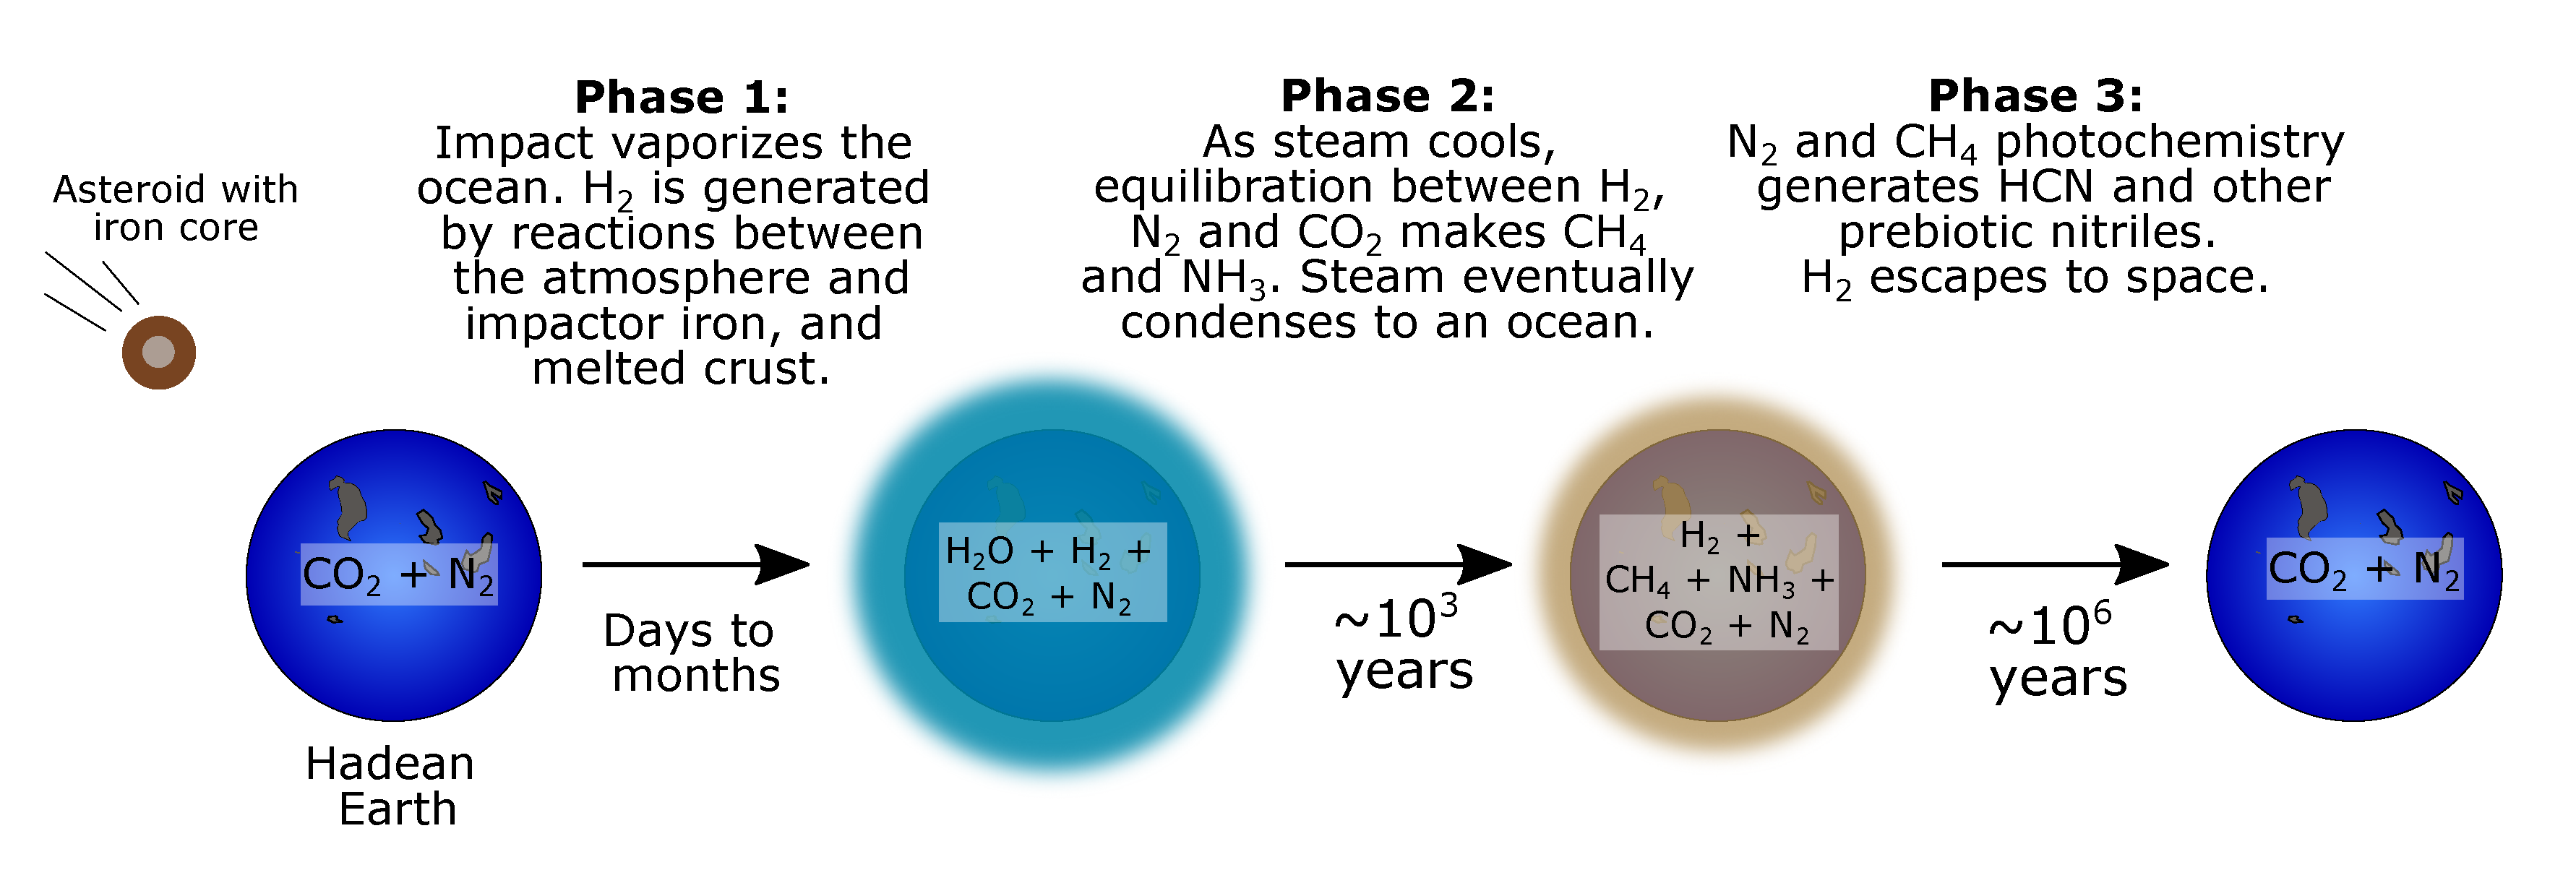
\includegraphics[width=1.0\textwidth]{tex/5impacts/figures/impact_diagram.pdf}
  \caption{The three phases of atmospheric evolution after a large asteroid impact on the Hadean Earth. In Phase 1, the impactor vaporizes the ocean and heats up the atmosphere. Iron delivered by the impactor reacts with hot steam to make H$_2$. H$_2$ is also modulated by equilibration between the atmosphere and an impact-generated melt pond. In Phase 2, as the steam-rich atmosphere cools for thousands of years, H$_2$ reacts with CO$_2$ to make atmospheric CH$_4$. Ultimately, the steam condenses to an ocean. Finally, in Phase 3, N$_2$ and CH$_4$ photochemistry generates HCN and other prebiotic nitriles. The H$_2$ dominated atmosphere escapes to space over millions of years, causing the return of a more oxidizing N$_2$ and CO$_2$ atmosphere.}
  \label{fig:impact_diagram}
\end{figure}

\subsection{Phase 1: Reducing the steam-generated atmosphere with impactor iron} \label{sec:phase1}

Within days, a massive asteroid impact would leave the Hadean Earth with a global $\sim$2000 K rock and iron vapor atmosphere, the iron derived from the impactor's core \citep{Itcovitz_2022}. In the following months to years, energy radiated downward from the silicates would vaporize a large fraction of the ocean, adding steam to the atmosphere \citep{Sleep_1989}. At this point, steam should rapidly react with iron to generate H$_2$. Eventually, the iron vapor and then rock would rain out leaving behind a steam-dominated atmosphere containing H$_2$, as well as CO$_2$ and N$_2$ from the pre-impact atmosphere. The sequence of metal followed by silicate condensation with falling temperature is loosely analogous to that of the well-known condensation sequence of the solar nebula.

Furthermore, the massive impact would generate a melt pool on Earth's surface inside the impact crater, which may contain reducing impact-derived iron. The atmosphere and melt pool could react to a redox-equilibrium state. This could add or sequester H$_2$ from the atmosphere, depending on whether the melt was more or less reducing than the atmosphere \citep{Itcovitz_2022}.

Recently, \citet{Itcovitz_2022} used a smoothed-particle hydrodynamics (SPH) code with $0.5 \times 10^6$ - $3 \times 10^6$ particles of 150 - 250 km diameter to estimate the amount of H$_2$ generated as these processes unfold under several different impact scenarios on the Hadean Earth. In their fiducial case (i.e. their ``Model 1A''), they assume that 100\% of iron delivered by an impactor is available to react and reduce a post-impact steam atmosphere. In another scenario, they assume that only $\sim$15 - 30\% of impactor iron reacts with the steam atmosphere based on their SPH simulations (their ``Model 1B'') \citep{Citron_2022}. For both cases, they also consider equilibration between the atmosphere and a melt pool (their ``Model 2'', ``Model 3A'' and ``Model 3B''). In their simulations, the melt pool is extremely reducing or more oxidizing depending on whether they assume it contains a fraction of the impactor's iron, and they use SPH models to predict the amount of iron accreted to the melt pool \citep{Citron_2022}. Overall, they conclude that melt-atmosphere equilibration generates about as much H$_2$ as their fiducial case as long as the iron delivered to the melt-atmosphere system can equilibrate. However, if iron delivered to the melt pool sinks into Earth and cannot react with the atmosphere, then approximately 2 - 10 times less H$_2$ is produced compared to their fiducial scenario (see the erratum in \citet{Itcovitz_2022}).

\citet{Itcovitz_2022} considers impactors between $2 \times 10^{21}$ and $2 \times 10^{22}$ kg, and assumes the pre-impact Earth has 1.85 oceans of water, 100 bars CO$_2$ and 2 bars of N$_2$. However, we investigate impacts as small as $10^{20}$ kg, and our nominal model (Table \ref{tab:fiducial_parameters}) assumes only 0.5 bars of pre-impact CO$_2$ motivated by models of the Hadean carbonate-silicate cycle \citep{Kadoya_2020} and assuming little mantle-hosted carbonate is vaporized. Therefore, we use a similar model (Appendix \ref{sec:phase1_appendix}) to the one described in \citet{Itcovitz_2022} to predict the post-impact H$_2$ for our alternative model assumptions (Table \ref{tab:fiducial_parameters}) and impactor sizes. Figure \ref{fig:melt_reaction_sup} shows the results.

\begin{figure}
  \centering
  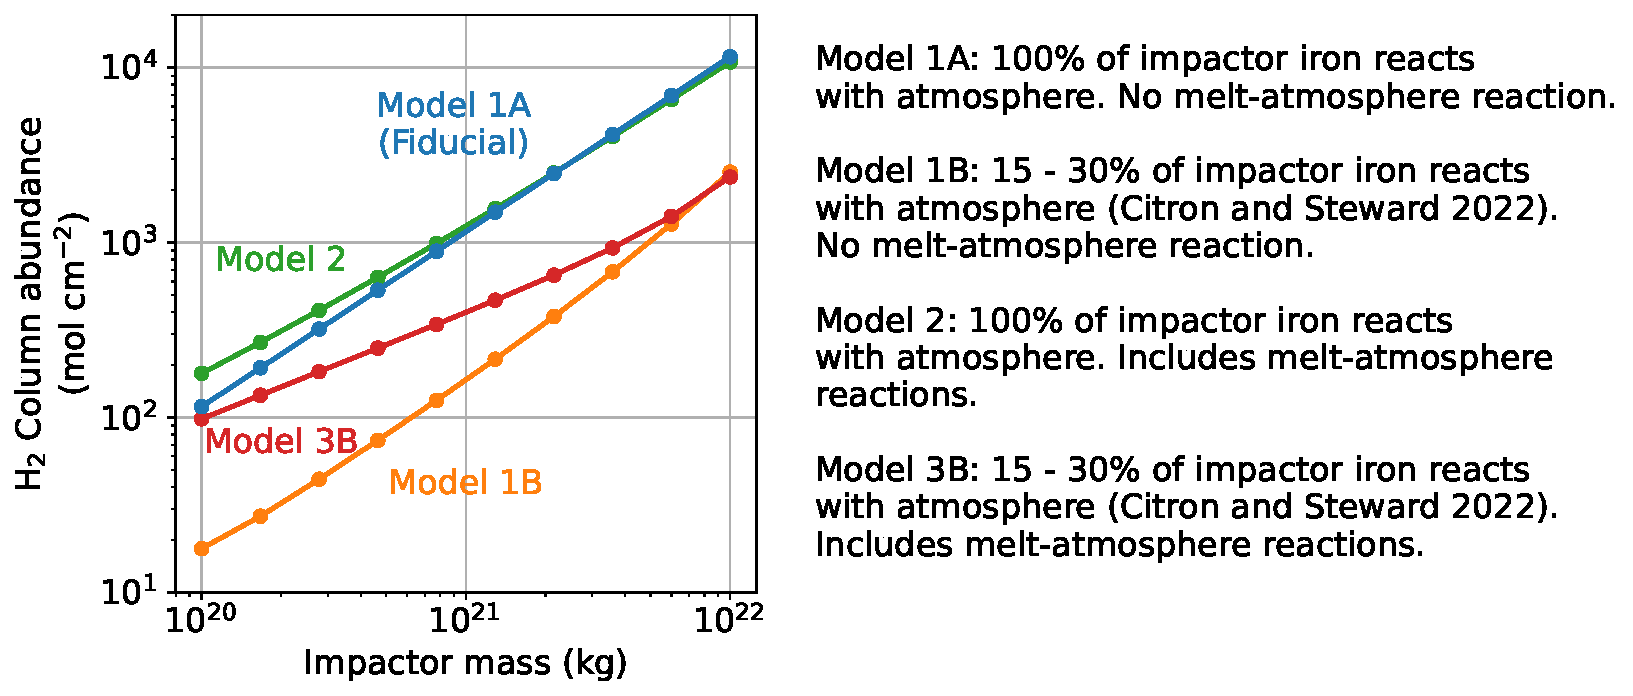
\includegraphics[width=0.95\textwidth]{tex/5impacts/figures/melt_reaction_sup.pdf}
  \caption{Post-impact H$_2$ generation as a function of impactor mass under different modeling assumptions. Models 1A, 1B, 2 and 3B are identical to those describe in Figure 1 of \citet{Itcovitz_2022}. The simulation's pre-impact volatile inventories, impact angle, and impact velocity are listed in Table \ref{tab:fiducial_parameters}. In Model 1A, all iron delivered by an impact reacts with steam to produce H$_2$. The resulting atmosphere does not equilibrate with a impact-generated melt pool. Model 1B assumes that a fraction ($\sim 15\%$ to $\sim 30\%$) of impactor iron reduces the steam atmosphere based on SPH simulations \citep{Citron_2022}, and that the atmosphere is chemically isolated from a melt pool. Model 2 is like Model 1A while also including post-impact equilibration with a melt pool with a redox state of $\Delta$FMQ-2.3 to represent peridotite \citep{Itcovitz_2022}. Model 3B assumes that a fraction ($\sim 15\%$ to $\sim 30\%$) of impactor iron reacts with the steam atmosphere based on SPH simulations, and includes melt-atmosphere redox equilibration with a pool magma initially at $\Delta$FMQ-2.3. As stated in Section \ref{sec:phase1}, we nominally assume Model 1A throughout the main text calculations. We also include simulations in the appendix that instead adopt Model 1B, which we consider to be a plausible lower bound for post-impact H$_2$ generation.}
  \label{fig:melt_reaction_sup}
\end{figure}

Our calculations give two end-member scenarios for impact H$_2$ production which we consider for subsequent calculations in this article. The more optimistic case assumes that 100\% of the impactor's iron reacts with an atmosphere that is chemically isolated from a melt pool (``Model 1A'' in Figure \ref{fig:melt_reaction_sup}). Following \citet{Zahnle_2020}, we adopt this scenario as our nominal model throughout the main text. This assumption produces a similar amount of H$_2$ as an atmosphere-melt system that retains most of the impactor's iron (e.g. ``Model 2'' in Figure \ref{fig:melt_reaction_sup}), which is consistent with \citet{Itcovitz_2022}. The ``Model 2'' calculation assumes the melt pool has an initial oxygen fugacity of $\Delta$FMQ-2.3 which is appropriate for a peridotite melt \citep{Itcovitz_2022}.\footnote{FMQ is the fayalite-magnetite-quartz redox buffer. See Chapter 7 in \citet{Catling_2017} for a discussion of redox buffers.} However, our results are not sensitive to this assumption because, for ``Model 2'', initial melt oxygen fugacities between $\Delta$FMQ and $\Delta$FMQ-4 changes the generated H$_2$ by a factor of at most $\sim 1.3$.

The less-optimistic case for H$_2$ production is ``Model 1B'' in Figure \ref{fig:melt_reaction_sup}, which assumes that only a fraction of the impactor iron reacts with an atmosphere, and that the latter does not react with a melt pool. We compute the fraction of available iron by extrapolating SPH simulations of impacts traveling at twice Earth's escape velocity and colliding with Earth at a 45$^{\circ}$ angle (Appendix Figure \ref{fig:citron_interpolations}), which is the most probable angle \citep{Citron_2022}. Most simulations shown in the main text have a complementary figure in the Appendix that makes this alternative pessimistic assumption regarding post-impact H$_2$ generation.

\begin{table}
  \caption{Nominal model assumptions}
  \label{tab:fiducial_parameters}
  \begin{center}
  \begin{tabularx}{0.9\linewidth}{p{0.3\linewidth} | p{0.2\linewidth} | p{0.3\linewidth}}
    \hline \hline
    Parameter & symbol & value \\
    \hline
    Pre-impact ocean inventory & $N_\mathrm{H_2O}$ & $1.5 \times 10^4$ mol cm$^{-2}$ (i.e. 1 ocean) 
    \\
    Pre-impact CO$_2$ inventory & $N_\mathrm{CO_2}$ & 12.5 mol cm$^{-2}$ (i.e. ``0.5 bars'') 
    \\
    Pre-impact N$_2$ inventory & $N_\mathrm{N_2}$ & 36 mol cm$^{-2}$ (i.e. ``1 bar'') 
    \\
    Impactor mass & $M_\text{imp}$ & $10^{20}$ - $10^{22}$ kg
    \\
    Iron mass fraction of the impactor & $m_\text{Fe,imp}$ & 0.33 
    \\
    Fraction of iron that reacts with atmosphere & $X_\mathrm{Fe,atmos}$ & 1.0$^{a}$ 
    \\
    Impact angle & - & 45$^{\circ}$
    \\
    Impact velocity relative to Earth & - & $20.7$ km s$^{-1}$
    \\
    Eddy diffusion coefficient$^\text{b}$ & $K_{zz}$ & $10^6$ cm$^{2}$ s$^{-1}$ 
    \\
    Aerosol particle radius$^\text{b}$ & - & 0.1 $\mu$m
    \\
    Troposphere relative humidity & $\phi$ & 1 
    \\
    Surface Albedo & $A_s$ & 0.2 
    \\
    Temperature of the stratosphere & T$_\mathrm{strat}$ & 200 K 
    \\
    Rainfall rate & $R_\mathrm{rain}$ & $1.1 \times 10^{17}$ molecules cm$^{-2}$ s$^{-1}$  (Modern Earth's value) 
    \\
    HCN deposition velocity$^\text{c}$ & $v_\mathrm{dep,HCN}$ & $7 \times 10^{-3}$ cm s$^{-1}$
    \\
    HCCCN deposition velocity$^\text{d}$ & $v_\mathrm{dep,HCCCN}$ & $7 \times 10^{-3}$ cm s$^{-1}$
    \\
    \hline
    \multicolumn{3}{p{0.9\linewidth}}{
    $^\text{a}$ This is the ``Model 1A'' scenario for H$_2$ production described near the end of Section \ref{sec:phase1} and in Figure \ref{fig:melt_reaction_sup}.

    $^\text{b}$ Assumed to be constant as a function of altitude.

    $^\text{c}$ Estimated based on the HCN hydrolysis rate in the ocean (Appendix \ref{sec:hcn_vdep}).

    $^\text{d}$ Assumed to the the same as HCN.
  }
  \end{tabularx}
  \end{center}
\end{table}

\subsection{Phase 2: The cooling post-impact steam atmosphere} \label{sec:phase2}

After reactions between impact-derived iron and steam produce H$_2$, the atmosphere would radiate at a rate determined by the optical properties of water vapor \citep{Zahnle_2020}. Chemical reactions would initially be rapid, forcing the whole atmosphere to chemical equilibrium. Methane is thermodynamically preferred at lower temperatures, so it should become more abundant as the atmosphere cools. Eventually the atmosphere would reach a temperature where the reactions producing methane would be extremely sluggish compared to the rate of atmospheric cooling. At this point, the methane abundance would freeze, or quench. Ammonia would exhibit the same behavior as methane by initially rising in abundance then quenching when kinetics become slow. After several thousand years, water vapor condenses and rains out of the atmosphere to form an ocean.

We use the 0-D kinetics-climate box model described in Appendix \ref{sec:kinetics_climate} to simulate these events. By simulating each elementary chemical reaction, the model automatically computes methane and ammonia quenching as the atmosphere cools and temperature-dependent reactions slow. We first consider gas-phase kinetics, and later we will also consider nickel-surface kinetics.

Figure \ref{fig:figure1} shows our model applied to a $1.58 \times 10^{21}$ kg ($\sim 900$ km diameter) impactor. As the steam cools, ammonia quenches when the atmosphere is $\sim 1200$ K, followed by CH$_4$ quenching at $\sim 950$ K. After quenching, nearly half of the total carbon in the atmosphere exists as CH$_4$. After 4200 years, the steam has largely rained out to form an ocean, leaving behind a H$_2$-dominated atmosphere containing CH$_4$ and NH$_3$. NH$_3$ is soluble in water, so a fraction should be removed from the atmosphere by dissolution in the newly formed ocean; however our simulations (e.g. Figure \ref{fig:figure1}) do not account for this effect. 

\begin{figure}
  \centering
  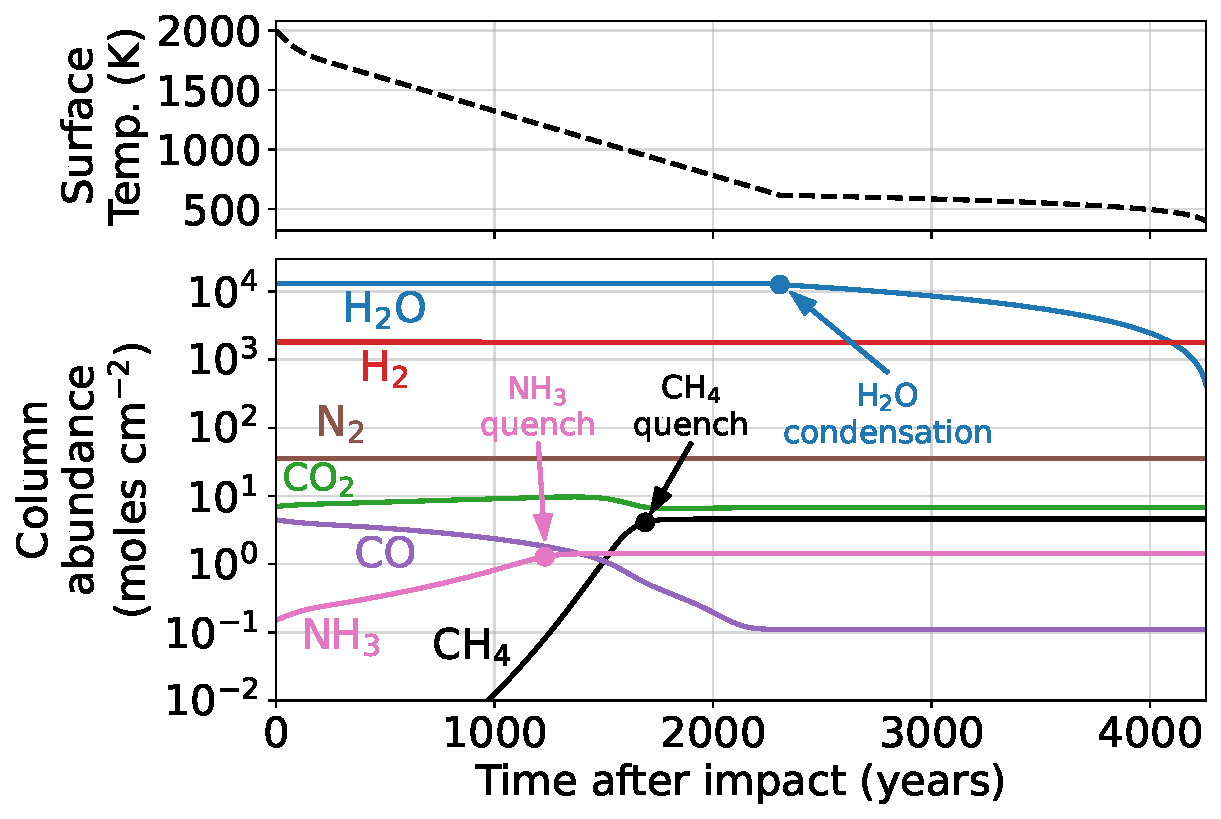
\includegraphics[width=0.7\textwidth]{tex/5impacts/figures/Figure1.pdf}
  \caption{A kinetics-climate simulation of a cooling steam atmosphere caused by a $1.58 \times 10^{21}$ kg impactor. The model uses the Table \ref{tab:fiducial_parameters} nominal parameters. The top panel is surface temperature and the bottom panel shows atmospheric composition.}
  \label{fig:figure1}
\end{figure}

Figure \ref{fig:figure2} shows predicted atmospheric composition at the end of the steam atmosphere (e.g. at 4200 years in Figure \ref{fig:figure1}) as a function of impactor mass. The calculations use gas-phase reactions, and our nominal model parameters (Table \ref{tab:fiducial_parameters}), including the assumption that 100\% of the iron delivered by the impactor reacts with the steam atmosphere to make H$_2$. For example, a $10^{20}$ kg impactor generates $1.2 \times 10^{2}$ H$_2$ moles cm$^{-2}$ which would have a partial pressure of 1.2 bars if the atmosphere did not contain water vapor. A $10^{22}$ kg impactor generates $1.1 \times 10^{4}$ H$_2$ moles cm$^{-2}$ which would have a ``dry'' partial pressure of 23.8 bars.\footnote{Partial pressures depend on the mean molecular weight of the atmosphere. The $10^{22}$ kg simulation in Figure \ref{fig:figure2} has 65.0 bars H$_2$ before ocean vapor condenses, and would have 23.8 bars H$_2$ if there was no water vapor in the atmosphere. Both scenarios have the same number of H$_2$ molecules in the atmosphere, but have different partial pressures because of dissimilar mean molecular weights. To avoid ambiguity, we occasionally report partial pressures in ``dry'' bars, which is the partial pressure of a gas if the atmosphere had no water vapor.}
We find that most of the CO$_2$ in the atmosphere is converted to CH$_4$ for impactors larger than $1.6 \times 10^{21}$ kg ($\sim 900$ km diameter), and that bigger impacts generate more NH$_3$, e.g., a $10^{22}$ kg impactor makes 0.013 ``dry'' bars of NH$_3$. Reduced species like CH$_4$ and NH$_3$ are thermodynamically preferred in the thick H$_2$ atmospheres generated by bigger impacts. Large impacts generate big amounts of hydrogen because they deliver more iron which more thoroughly reduces the atmosphere.

\begin{figure}
  \centering
  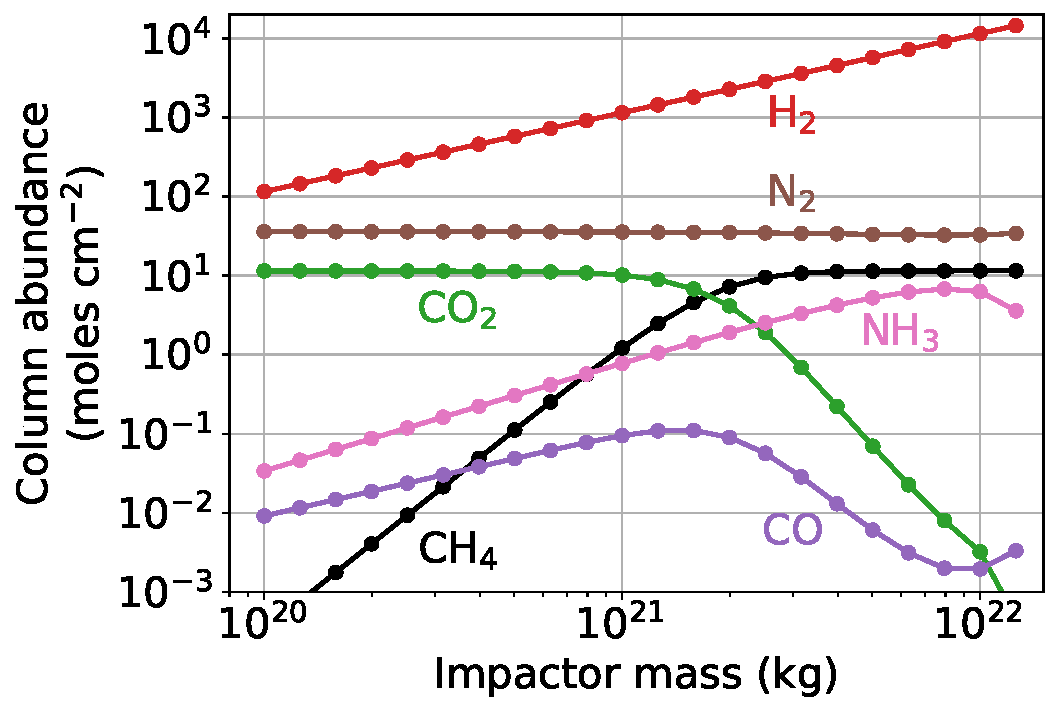
\includegraphics[width=0.65\textwidth]{tex/5impacts/figures/Figure2.pdf}
  \caption{Predicted atmospheric composition as a function of impactor mass after steam has condensed to an ocean. We use our nominal modeling assumptions (Table \ref{tab:fiducial_parameters}), and also use gas-phase kinetics. Most CO$_2$ is converted to CH$_4$ for impactors larger than $1.6 \times 10^{21}$ kg.}
  \label{fig:figure2}
\end{figure}

The Figure \ref{fig:figure2} calculations might underestimate the CH$_4$ produced in the post-impact atmosphere because they ignore reactions occurring on nickel surfaces that can catalyze CH$_4$ generation. If the impactors that struck the Earth during the Hadean resembled enstatite chondrite or carbonaceous chondrite composition then they would have contained 1\% - 2\% nickel \citep[Table 15]{Lewis_1992}. This nickel would have coexisted with the rock and iron vapor atmosphere that lasted months to years following a massive impact (Phase 1 in Figure \ref{fig:impact_diagram}). Metals along with silicates would have rained out as spherules covering the entire planet \citep{Genda_2017}. As the impact-generated steam cooled, chemical reactions catalyzing CH$_4$ production could have occurred on nickel surfaces in the bed of spherules \citep{Schmider_2021}. These surface reactions could lower the quench temperature of CH$_4$, causing more of the gas to be produced.

To estimate the effect of nickel catalysis on CH$_4$ production, we use our kinetics-climate model box model (Appendix \ref{sec:kinetics_climate}) with the nickel-surface reaction network developed by \citet{Schmider_2021}. The network is based on quantum chemistry calculations and about a dozen experiments from the literature. Our micro-kinetics approach is distinct from the empirical one taken by, e.g. \citet{Kress_2004}, because our model tries to capture each elementary step of catalysis, rather than use a parameterization that is specific to certain experimental conditions. 

Figure \ref{fig:figure3} shows the quenched methane abundance as a function of impactor mass predicted by our model that includes nickel catalysts. The amount of CH$_4$ generated depends strongly on the amount of available nickel surface area. Nickel areas bigger than 0.1 cm$^2$ nickel / cm$^2$ Earth permit more CH$_4$ production compared to our gas-phase only model. Assuming a nickel area of 1000 cm$^2$ nickel / cm$^2$ Earth, then a Vesta-size impactor ($2.6 \times 10^{20}$ kg, 500 km diameter) could convert most CO$_2$ in the pre-impact atmosphere to CH$_4$.

Unfortunately, a precise nickel surface area is hard to estimate. The correct value depends on how the rock, iron and nickel spherules mix and precipitate to the surface, and furthermore, how effectively the atmosphere can diffuse through and react on exposed nickel. We do not attempt to compute these effects here, and instead estimate possible upper bounds. Consider a $2.6 \times 10^{20}$ kg impactor (Vesta-sized) of enstatite chondrite composition, containing 2\% by mass Ni \citep{Lewis_1992}. If all this nickel is gathered into 1 mm spheres, a plausible droplet size according to \citet{Genda_2017}, then the total nickel surface area is $3.4 \times 10^3$ cm$^2$ nickel / cm$^2$ Earth. An impactor ten times more massive would deliver ten times more nickel resulting in an upper bound Ni area that is one order of magnitude larger. Significantly smaller nickel particles are conceivable. There is experimental support for the formation of ultra-fine $< 300$ nm particles in the wake of impacts colliding with an ocean \citep{Furukawa_2007}. For a Vesta-sized impactor, collecting all nickel into $100$ nm particles has a nickel area five orders of magnitude large than the 1 mm case - $3.4 \times 10^{9}$ cm$^2$ nickel / cm$^2$ Earth. Overall, the larger nickel areas shown in Figure \ref{fig:figure3} may be within the realm of possibility.

\begin{figure}
  \centering
  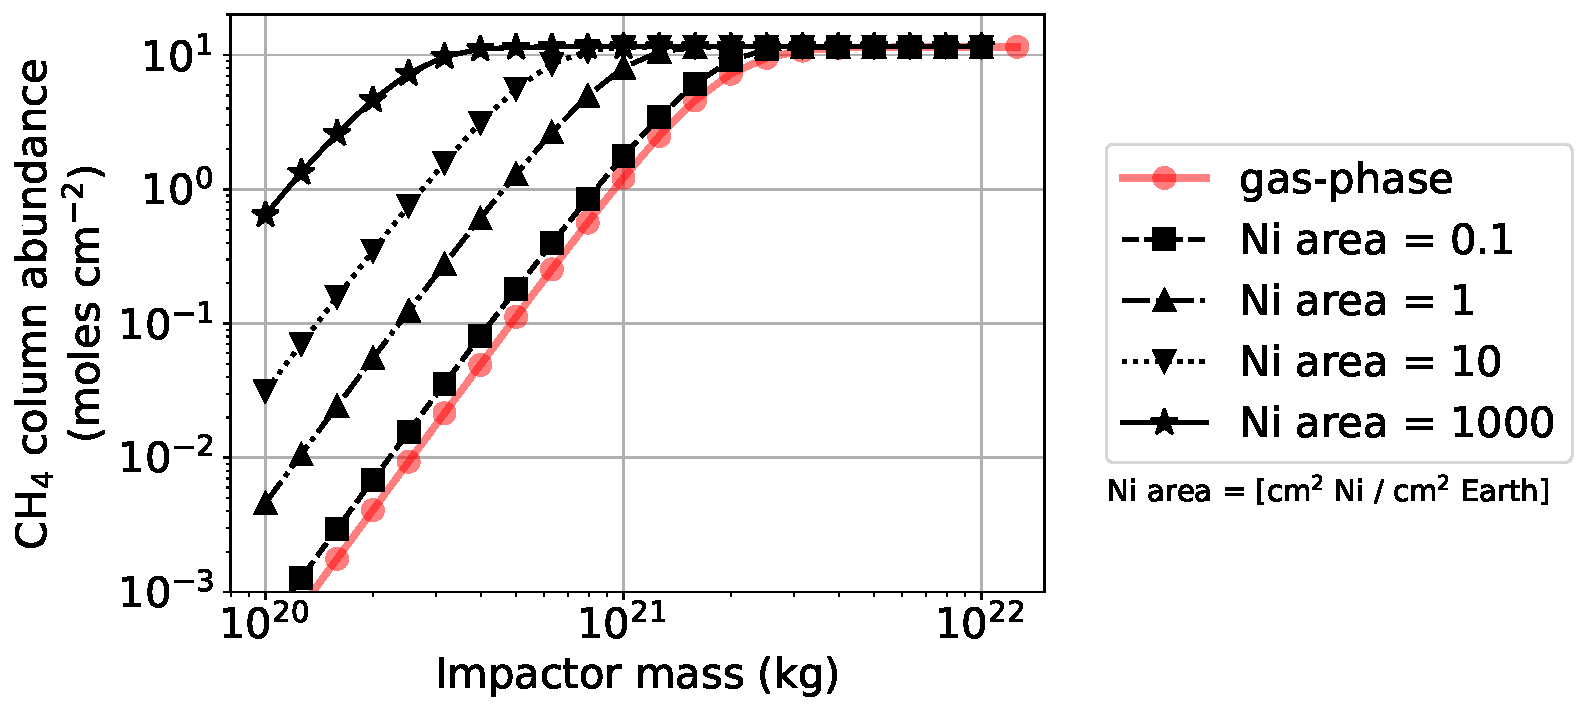
\includegraphics[width=0.8\textwidth]{tex/5impacts/figures/Figure3.pdf}
  \caption{The effect of nickel catalysts on post-impact methane production. The calculations use the Table \ref{tab:fiducial_parameters} model parameters and the \citet{Schmider_2021} surface reaction network. Ni areas larger than 0.1 cm$^2$ nickel / cm$^2$ Earth generates more methane than our model that uses gas-phase reactions, e.g., Figure \ref{fig:figure2}.}
  \label{fig:figure3}
\end{figure}

Figures \ref{fig:figure2} and \ref{fig:figure3} optimistically assume that all iron delivered by the impactor reacts with steam to make H$_2$, however, this may not be the case (see Section \ref{sec:phase1}). Therefore, in Appendix Figures \ref{fig:figure2_citron} and \ref{fig:figure3_citron} we recalculate Figures \ref{fig:figure2} and \ref{fig:figure3}, but assume that only a fraction of the impactor's iron reduces the steam atmosphere by extrapolating SPH simulations of impacts (``Model 1B'' in Figure \ref{fig:melt_reaction_sup}). The resulting H$_2$, CH$_4$, and NH$_3$ production appear similar, except shifted by a factor of $\sim 5$ to larger impactors. The results are shifted by this amount because SPH simulations suggest approximately $\sim 1/5$ of impactor iron is delivered to the atmosphere, while the rest is either embedded in Earth, or ejected to space. We consider these supplementary calculations lower-bounds for impactor generated CH$_4$ and NH$_3$.

\subsection{Phase 3: Long-term photochemical-climate evolution} \label{sec:phase3}

Several thousand years after a massive impact, the steam-dominated atmosphere would condense to an ocean leaving behind a H$_2$-dominated atmosphere containing CH$_4$ and NH$_3$ (e.g. at 4200 years in Figure \ref{fig:figure1}). The reducing atmospheric state should persist for millions of years until hydrogen escapes \citep{Zahnle_2020}.

\begin{figure}
  \centering
  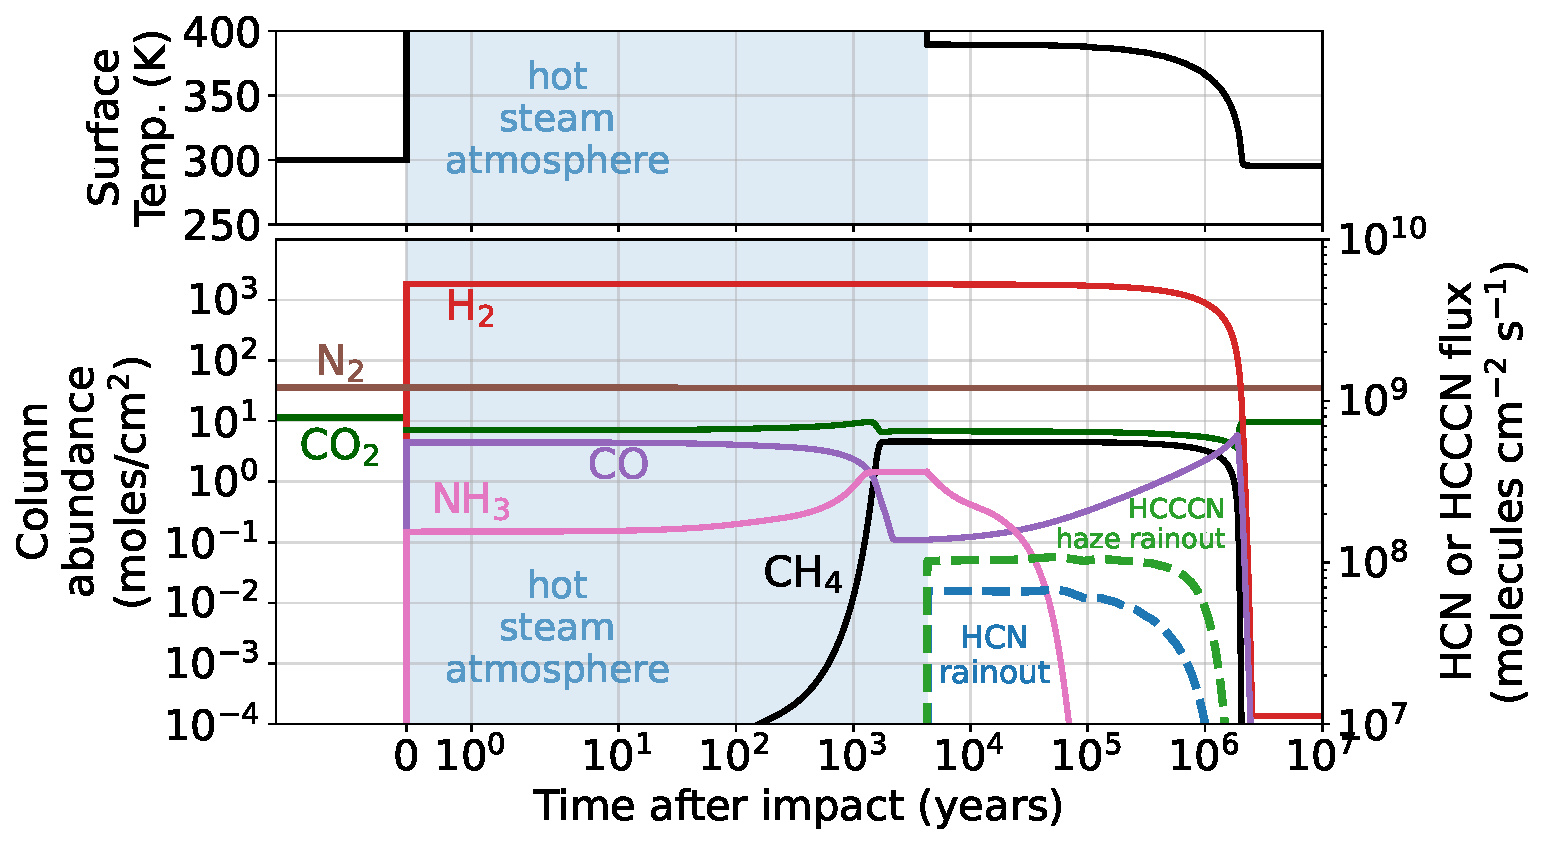
\includegraphics[width=0.9\textwidth]{tex/5impacts/figures/Figure4.pdf}
  \caption{Simulated composition and climate of the Hadean atmosphere after a $1.58 \times 10^{21}$ kg impactor that produces 7.0 bars of H$_2$ once vaporized ocean water condenses. We use the Table \ref{tab:fiducial_parameters} model parameters. The blue shaded region labeled ``hot steam atmosphere'', also called Phase 2 in Figure \ref{fig:impact_diagram}, is simulated by the kinetics-climate model described in Appendix \ref{sec:kinetics_climate}. After this time-period, during Phase 3 of a post-impact atmosphere, we evolve the atmosphere with 1-D photochemical-climate model (Appendix \ref{sec:photochem}), which maintains 0.018 bar of CH$_4$ between $4 \times 10^3$ and $\sim 10^6$ years. Dashed lines are referenced to the right-hand axis. ``HCN rainout'' is HCN molecules raining out in droplets of water. ``HCCCN haze rainout'' is the rainout rate of HCCCN incorporated into particles formed from the reaction $\mathrm{C_4H} + \mathrm{HCCCN} \rightarrow \mathrm{polymer}$. CH$_4$ and N$_2$ photochemistry generates HCN and HCCCN for about one million years until H$_2$ escapes to space.}
  \label{fig:figure4}
\end{figure}

We simulate the long-term evolution of this hydrogen-rich atmosphere using a coupled one-dimensional photochemical-climate model (Appendix \ref{sec:photochem}). Figure \ref{fig:figure4} shows our model applied to the atmosphere following a $1.58 \times 10^{21}$ kg ($\sim 900$ km diameter) impactor. We assume a pre-impact atmosphere with 1 bar N$_2$ and 0.5 bars of CO$_2$, and simulate the cooling steam atmosphere with our kinetics-climate climate model (Section \ref{sec:phase2}). Next, we use the end of the steam atmosphere simulation as initial conditions for our 1-D photochemical-climate model. 

We find that N$_2$ and CH$_4$ photochemistry generates HCN in a hazy Titan-like atmosphere for about one million years until it is halted by hydrogen escape to space. In this model, the dominant channel producing HCN is $\mathrm{N} + \mathrm{^3CH_2} \rightarrow \mathrm{HCN} + \mathrm{H}$ where $\mathrm{^3CH_2}$ is ground (triplet) state of the methylene radical derived form methane photolysis. There are two other important paths. The first is $\mathrm{N} + \mathrm{CH} \rightarrow \mathrm{CN} + \mathrm{H}$ followed by $\mathrm{H_2} + \mathrm{CN} \rightarrow \mathrm{HCN} + \mathrm{H}$, and the second is $\mathrm{N} + \mathrm{CH_3} \rightarrow \mathrm{H} + \mathrm{H_2CN}$ and $\mathrm{H_2CN} + \mathrm{H} \rightarrow \mathrm{HCN} + \mathrm{H_2}$. In all pathways, hydrocarbon radicals (e.g., $\mathrm{^3CH_2}$ and $\mathrm{CH_3}$) are sourced from photolyzed CH$_4$ and atomic N is derived from photolyzed N$_2$, which both occur at high altitudes ($p < 10^{-5}$ bar, Appendix Figure \ref{fig:ch4_n_hcn}). The largest chemical loss of HCN is photolysis followed by $\mathrm{N} + \mathrm{CN} \rightarrow \mathrm{N_2} + \mathrm{C}$. Other significant losses are paths that form HCCCN aerosols. HCN production and loss is our model is comparable to pathways discussed in similar studies \citep{Zahnle_1986,Tian_2011,Rimmer_2019}.

In Figure \ref{fig:figure4}, HCN mixes to the surface and rains out in droplets of water at a rate of $\sim 10^7$ molecules cm$^{-2}$ s$^{-1}$. HCN also dissolves into the ocean at a similar rate, where we assume it is eventually destroyed by hydrolysis (not shown in Figure \ref{fig:figure4}). To emulate HCN dissolution and destruction in the ocean, we assume a $7 \times 10^{-3}$ cm s$^{-1}$ deposition velocity justified in Appendix \ref{sec:hcn_vdep}. Additionally, a relatively small amount of HCN polymerizes to haze particles in our model via $\mathrm{H_2CN} + \mathrm{HCN} \rightarrow \mathrm{polymer}$ following \citet{Lavvas_2008}, which falls and rains out in water droplets to the surface.

Our results differ from the simulations of \citet{Zahnle_2020}, which suggested that the duration of HCN production after an impact was limited by rapid photolysis of methane. The Figure \ref{fig:figure4} simulation finds that the CH$_4$ lifetime is 4.8 million years because, following photolysis, CH$_4$ efficiently recombines in a hydrogen rich atmosphere from the following reaction, which is well known in the atmospheres of the giant planets in out solar system (Appendix Figure \ref{fig:ch4_prod_loss}).

\begin{equation} \label{eq:ch4_recom}
  \mathrm{CH_3} + \mathrm{H} + \mathrm{M} \rightarrow \mathrm{CH_4} + \mathrm{M}  
\end{equation}
\citet{Zahnle_2020} did not account for Reaction \ref{eq:ch4_recom}. The lifetime of cyanide production is therefore instead determined by the timescale of hydrogen escape to space. Significant hydrogen escape permits the destruction of most atmospheric CH$_4$ because Reaction \ref{eq:ch4_recom} becomes inefficient, which in turn ceases CH$_4$-driven HCN production.

In Figure \ref{fig:figure4}, HCCCN is primarily destroyed by photolysis and produced by the following reaction from acetylene and the cyanide radical,

\begin{equation} \label{eq:hcccn}
  \mathrm{C_2H_2} + \mathrm{CN} \rightarrow \mathrm{HCCCN} + \mathrm{H}  
\end{equation}
A fraction of produced HCCCN reacts to form aerosols via $\mathrm{C_4H} + \mathrm{HCCCN} \rightarrow \mathrm{polymer}$ following \citet{Lavvas_2008}. These polymers fall and mix toward the surface where they rainout in droplets of water at a rate of $\sim 10^{8}$ molecules cm$^{-2}$ s$^{-1}$. Most gas-phase HCCCN is either destroyed by photolysis or incorporated into aerosols, causing vanishingly small surface HCCCN gas pressures ($< 10^{-{16}}$ bar).

In Figure \ref{fig:figure4}, impact-generated ammonia persists for nearly $10^5$ years. NH$_3$ is primarily destroyed by photolysis, but then recombines from reactions with hydrogen:

\begin{gather} 
  \mathrm{NH} + \mathrm{H_2} + \mathrm{M} \rightarrow \mathrm{NH_3} + \mathrm{M} \label{eq:nh3_1} 
  \\
  \mathrm{NH_2} + \mathrm{H} + \mathrm{M} \rightarrow \mathrm{NH_3} + \mathrm{M} \label{eq:nh3_2}
\end{gather}
Reactions \ref{eq:nh3_1} and \ref{eq:nh3_2} are relatively efficient in a hydrogen-rich atmosphere. Ammonia photolyisis primarily occurs at the $10^{-3}$ bar altitude, while haze is largely produced above the $10^{-5}$ bar altitude. Therefore, haze particles partially shield ammonia from photolysis, extending the NH$_3$ lifetime \citep{Sagan_1997}. Our model assumes the haze particles are perfect spheres with optical properties governed by Mie theory. Observations of Titan's haze have revealed that hydrocarbon haze particles have a fractal structure which absorb and scatter UV more effectively than Mie spheres \citep{Wolf_2010}. Therefore, our model likely overestimates NH$_3$ photolysis in post-impact atmospheres. 

Figure \ref{fig:figure4} assumes that all NH$_3$ is in the atmosphere and that it does not rainout, but the gas is highly soluble in water and should dissolve in the ocean where it hydrolyzes to ammonium, NH$_4^+$. \citet{Zahnle_2020} showed that NH$_3$ partitioning between the atmosphere and ocean depends on ocean temperature and pH. For an atmosphere with 1.56 bars of total NH$_3$ and a 373 K ocean at $\text{pH} = 7.8$, \citet{Zahnle_2020} finds that $\sim 1\%$ of NH$_3$ would persist in the atmosphere, while the rest is dissolved in the ocean. Ammonia dissolution in the ocean would protect it from photolysis perhaps lengthening the lifetime of ammonia in the atmosphere-ocean system. Overall, since our model neglects NH$_3$ ocean dissolution and likely overestimates NH$_3$ photolysis, then we probably underestimate the lifetime of NH$_3$ in Figure \ref{fig:figure4}.

While HCN and HCCCN are produced in Figure \ref{fig:figure4}, the surface temperature would be $\sim 390$ K primarily caused by H$_2$-H$_2$ collision-induced absorption (CIA), which has a significant greenhouse effect in thick H$_2$ atmospheres like this one of 8.5 bars total pressure. The atmosphere cools to $\sim 300$ K after H$_2$ escapes to space.

\begin{figure}
  \centering
  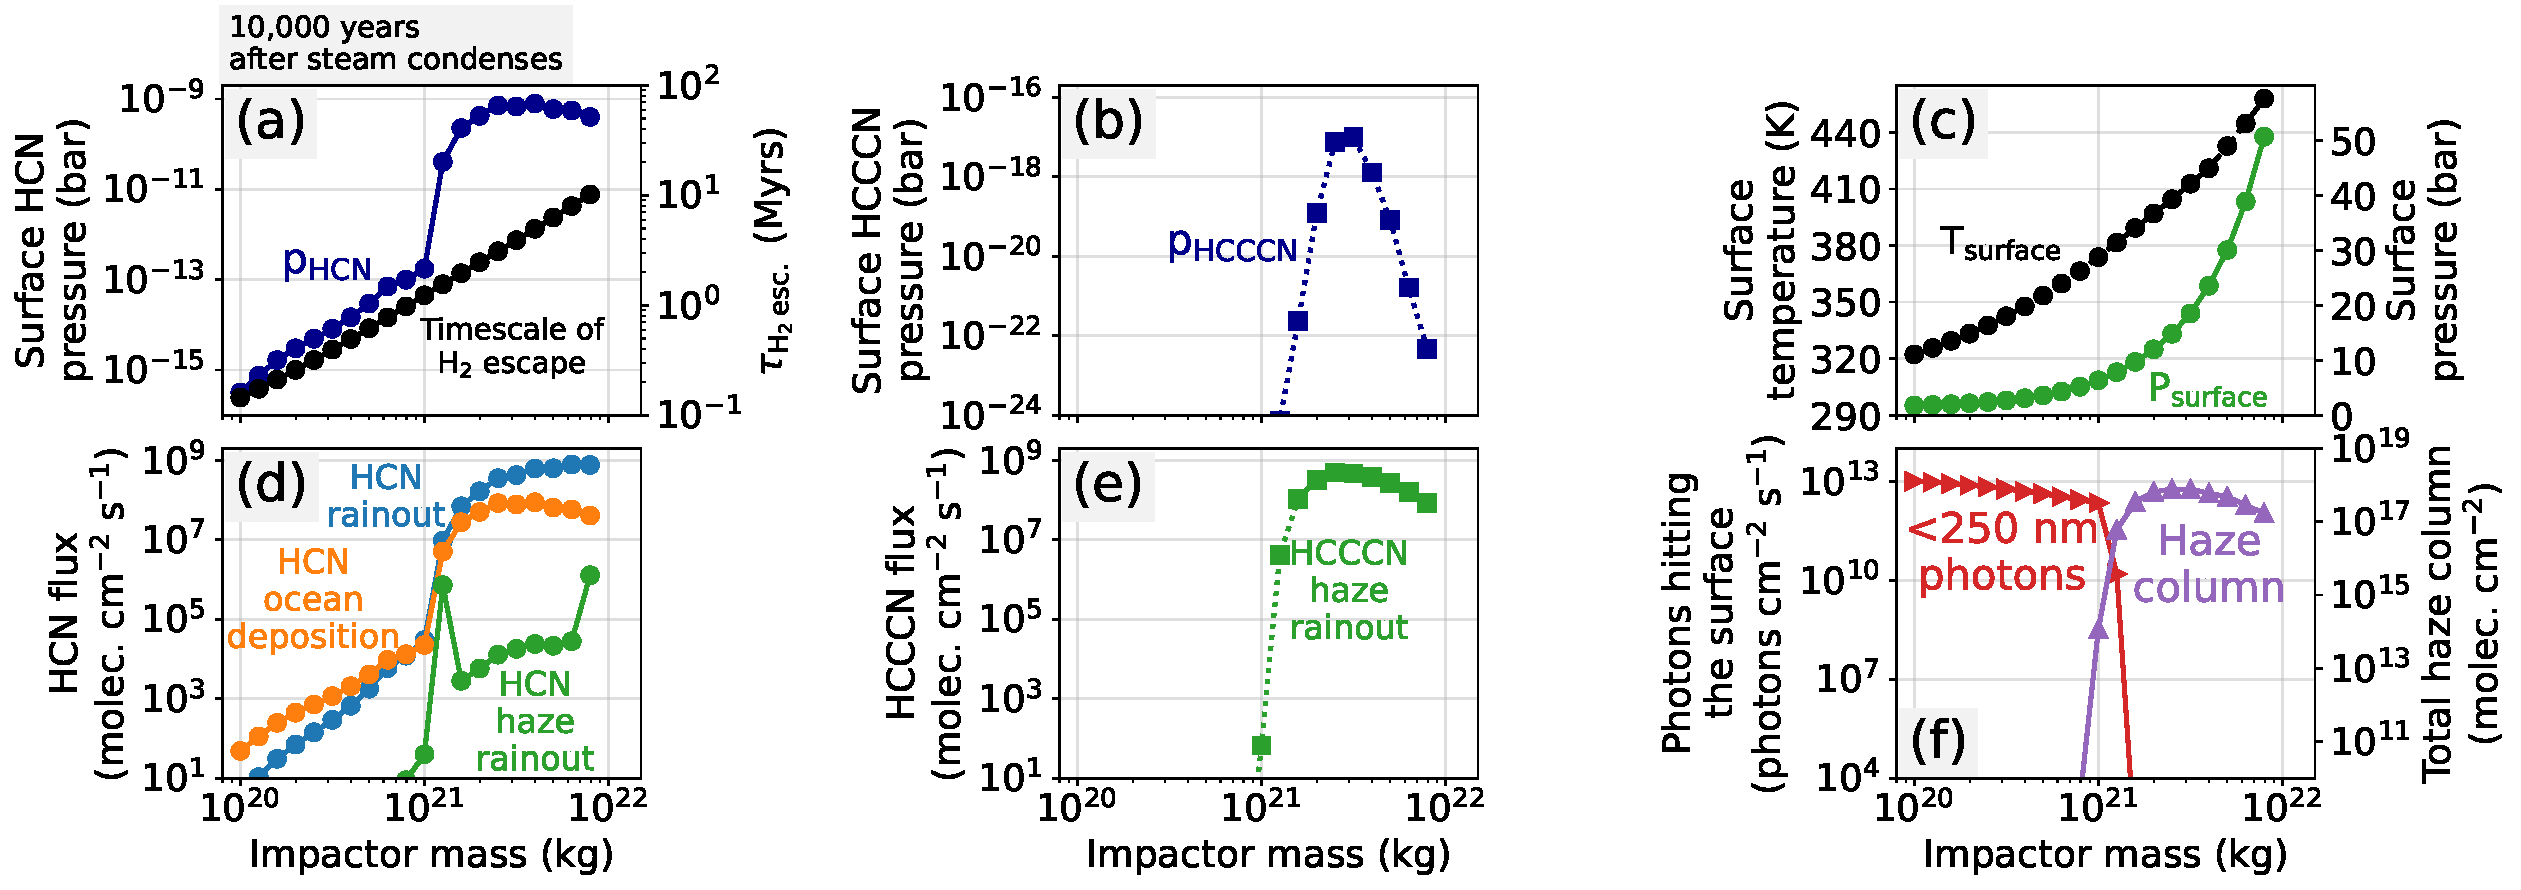
\includegraphics[width=1.0\textwidth]{tex/5impacts/figures/Figure5.pdf}
  \caption{The state of the Hadean post-impact atmospheres 10,000 years after steam condenses to an ocean. This time period is within Phase 3 of a post-impact atmosphere indicated in Figure \ref{fig:impact_diagram}. The simulations assume the Table \ref{tab:fiducial_parameters} parameters and gas-phase reactions during the cooling steam atmosphere. (a) The surface HCN pressure and timescale of H$_2$ escape, which can be interpreted as the approximate duration of HCN and HCCCN production. (b) The HCCCN surface pressure. (c) The surface temperature and pressure. (d) The HCN deposition rate in the ocean and the rate HCN leaves the atmosphere in rain drops. ``HCN haze rainout'' is the rainout rate of a aerosol created via the reaction $\mathrm{H_2CN} + \mathrm{HCN} \rightarrow \mathrm{polymer}$. (e) The rainout rate of an aerosol formed from the reaction $\mathrm{C_4H} + \mathrm{HCCCN} \rightarrow \mathrm{polymer}$. (f) The $< 250$ nm photons hitting the surface, and the total hydrocarbon haze column abundance. Impactors larger than $10^{21}$ kg produce haze-rich atmospheres and a stepwise increase in HCN and HCCCN production.}
  \label{fig:figure5}
\end{figure}

Figure \ref{fig:figure5} applies our model to various impactor masses. The results show the Hadean atmosphere 10,000 years after the post-impact generated steam atmosphere has condensed to an ocean. We choose 10,000 years after ocean condensation because this is adequate time for the atmosphere to reach a quasi-photochemical steady-state that does not change significantly until hydrogen escapes (e.g. Figure \ref{fig:figure4}). Figure \ref{fig:figure5}d and \ref{fig:figure5}e show a sharp increase in the HCN and HCCCN production for impactors larger than $10^{21}$ kg ($\sim 780$ km). Such large impacts generate $\mathrm{CH_4}/\mathrm{CO_2} > 0.1$ (Figure \ref{fig:figure2}), which makes a thick Titan-like haze \citep{Trainer_2006}. Haze shielding causes CH$_4$ photolysis to be higher in the atmosphere and closer to N$_2$ photolysis, therefore the photolysis products of both species can more efficiently combine to make cyanides (Appendix Figure \ref{fig:ch4_n_hcn}). Additionally, HCCCN production requires acetylene (Reaction \ref{eq:hcccn}), which is a haze precursor that accumulates when $\mathrm{CH_4}/\mathrm{CO_2} > 0.1$. These Titan-like atmospheres have $\sim 10^{-9}$ bar surface HCN, and HCN ocean deposition and rainout rates between $10^7$ and $10^9$ HCN molecules cm$^{-2}$ s$^{-1}$ persisting on hydrogen escape timescales ($> 1$ million years). HCCCN is incorporated into aerosols before raining out to the surface at a rate of up to $10^9$ HCCCN molecules cm$^{-2}$ s$^{-1}$.

In addition to photochemistry, lightning should also generate HCN \citep{Chameides_1981,Stribling_1987}. Appendix Figure \ref{fig:figure5_lightning} shows HCN production from lighting for the same time period as the Figure \ref{fig:figure5} simulation using methods described in \citet{Chameides_1981}. Assuming the same lightning dissipation rate as modern Earth's, we find that lightning produces up to $\sim 10^{4}$ HCN molecules cm$^{-2}$ s$^{-1}$. This value is small compared to the $10^{7}$ - $10^{9}$ HCN molecules cm$^{-2}$ s$^{-1}$ produced from photochemistry after $> 10^{21}$ kg impacts.

Larger impacts generate a thicker H$_2$ atmosphere which make the atmosphere warmer (Figure \ref{fig:figure5}c). For impactors $> 10^{21}$ kg, which generate substantial HCN and HCCCN, the surface temperature is $> 380$ K. Figure \ref{fig:figure5}f shows that impactors that produce substantial haze shield the surface from $< 250$ nm photons, which means that prebiotic schemes that require high energy UV light \citep[e.g.,][]{Patel_2015} would need to rely on stockpiling of the nitriles for later use. 

The Hadean Earth CO$_2$ concentration is uncertain. Models of the Hadean geologic carbon cycle argue for CO$_2$ levels between $\sim 10^{-5}$ and $1$ bar at 4 Ga with a median value of $\sim 0.5$ bar and a 95\% uncertainty spanning $10^{-5}$ to $1$ bar \citep{Kadoya_2020}. However, these values might be unrealistically small because a large impact would warm surface rocks possibly causing carbonates to degass thereby increasing the atmospheric CO$_2$ reservoir. Up to $\sim 80$ bars of CO$_2$ may potentially be liberated from surface carbonates \citep{KrissansenTotton_2021}.

\begin{figure}
  \centering
  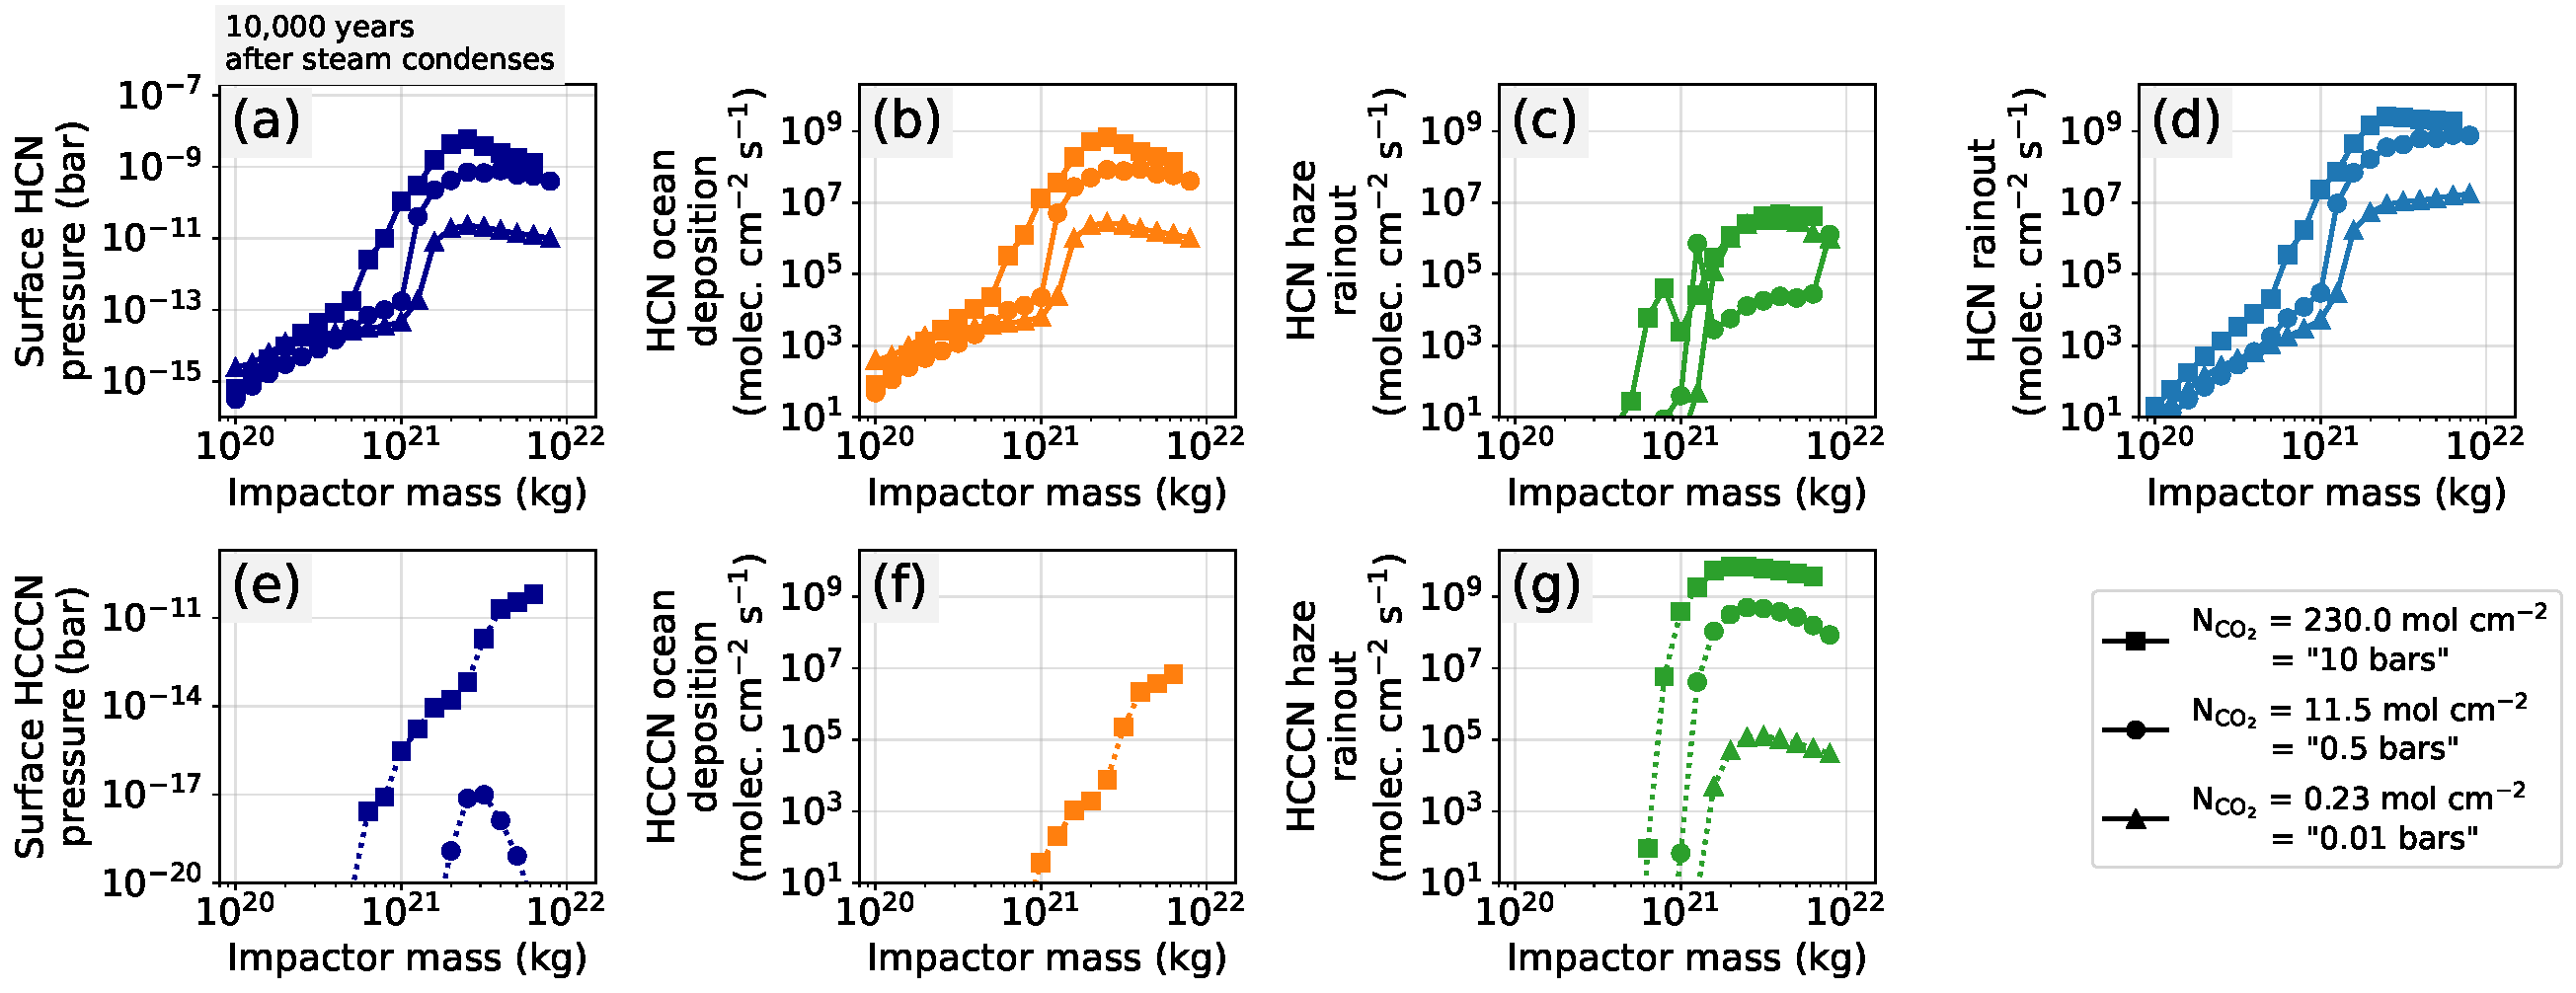
\includegraphics[width=1.0\textwidth]{tex/5impacts/figures/Figure6.pdf}
  \caption{The effect of the pre-impact CO$_2$ abundance on HCN and HCCCN production in post-impact atmospheres. All values are for the atmosphere 10,000 years after the steam condenses to an ocean, which is within Phase 3 of a post-impact atmosphere (Figure \ref{fig:impact_diagram}). The simulations assume the Table 1 parameters, except vary the pre-impact CO$_2$ inventory between 0.01 bar (triangles), 0.5 bar (circles), and 10 bars (squares). The calculations use gas-phase chemistry during the cooling steam atmosphere. Panels (a) - (d) show the surface HCN abundance and fluxes, while (e) - (g) show HCCCN production. Our model assumes that HCCCN is not soluble in water and does not rainout, therefore we omit a panel showing HCCCN rainout. Prebiotic nitrile production is directly correlated with the pre-impact CO$_2$ inventory.}
  \label{fig:figure6}
\end{figure}

Figure \ref{fig:figure6} explores the effect of different pre-impact CO$_2$ abundances on HCN and HCCCN production in post-impact atmospheres. The simulations are snapshots of the atmosphere 10,000 years after the impact-vaporized steam has condensed to an ocean. Larger pre-impact CO$_2$ causes larger HCN and HCCCN production because it allows more CH$_4$ to form in the cooling steam atmosphere. As discussed previously, CH$_4$ is closely tied to photochemical cyanide generation. Regardless of the pre-impact CO$_2$ concentrations, HCN and HCCCN production sharply increases for impactors larger than $\sim 10^{21}$ kg due to more efficient haze production (Figure \ref{fig:figure5}, and corresponding text).

\begin{figure}
  \centering
  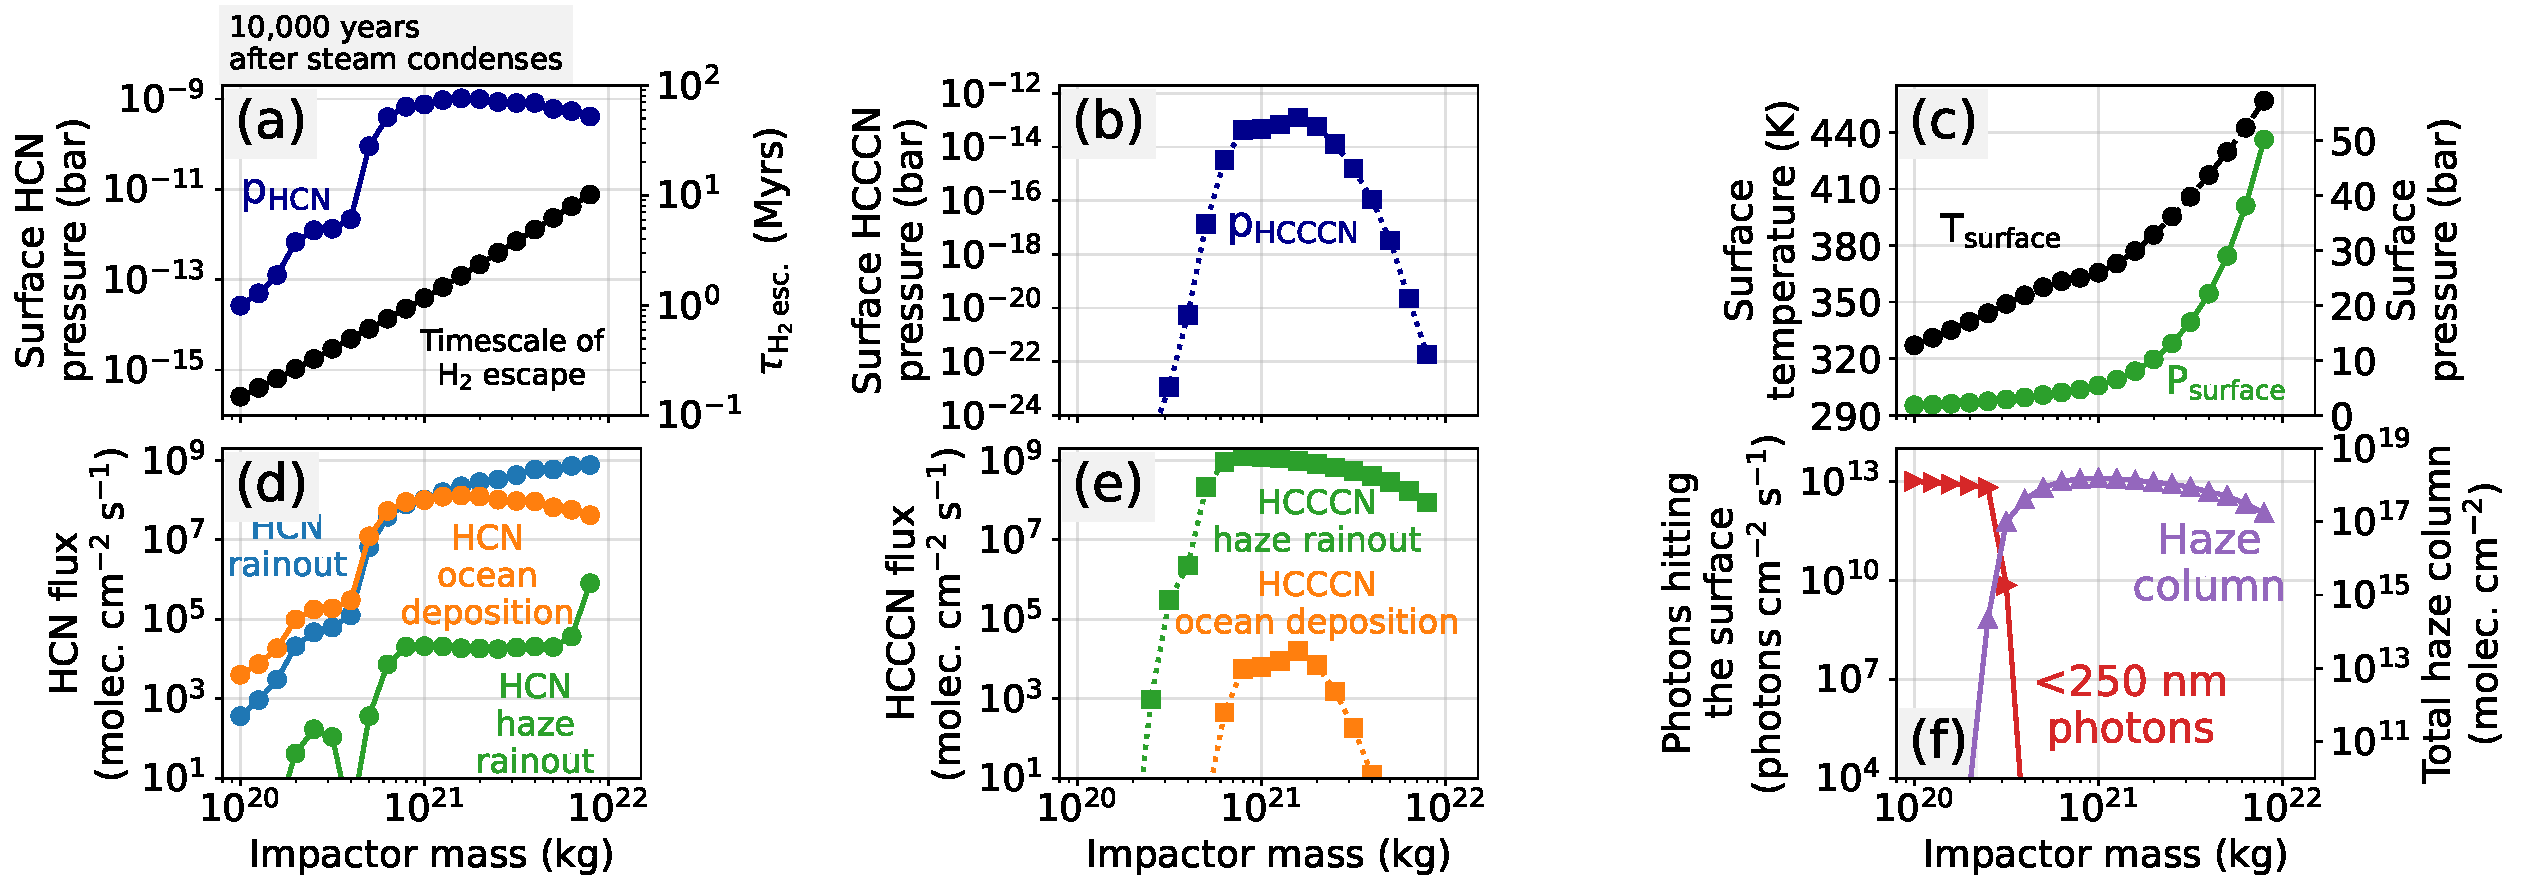
\includegraphics[width=1.0\textwidth]{tex/5impacts/figures/Figure7.pdf}
  \caption{Identical to Figure \ref{fig:figure5}, except simulations account for nickel-surface reactions which catalyze methane production as the steam atmosphere cools \citep{Schmider_2021}. We assume a nickel surface area of 10 cm$^2$ nickel / cm$^2$ Earth (for context, see Figure \ref{fig:figure3}). Nickel catalysts cause more efficient CH$_4$ generation, permitting bigger HCN and HCCCN production for smaller impactors compared to the gas-phase only scenario (Figure \ref{fig:figure5}).}
  \label{fig:figure7}
\end{figure}

Figure \ref{fig:figure7} shows the state of the atmosphere after impacts of various size assuming 10 cm$^2$ nickel / cm$^2$ Earth is present in the steam atmosphere to catalyze methane production. The nickel causes more efficient conversion of CO$_2$ to CH$_4$ compared to the gas-phase only scenario (Figure \ref{fig:figure5}) permitting bigger HCN and HCCCN for smaller impactors. For example, a $5 \times 10^{20}$ kg ($\sim 610$ km) impactor which accounts for nickel catalysts (Figure \ref{fig:figure7}) has comparable HCN and HCCCN production to a $1.6 \times 10^{21}$ kg ($\sim 900$ km diameter) impactor if no nickel catalysts are assumed in the cooling steam atmosphere (Figure \ref{fig:figure5}).

A critical assumption in this section is that 100\% of the iron delivered by impactors reacts with steam to generate H$_2$. As discussed in Section \ref{sec:phase1}, it is possible that the post-impact atmosphere is less thoroughly reduced by impactor iron. Appendix Figures \ref{fig:figure5_citron} and \ref{fig:figure7_citron} recalculate main text Figures \ref{fig:figure5} and \ref{fig:figure7}, assuming that a fraction (approximately 15\% to 30\%) of impactor iron reduces the steam atmosphere based on SPH simulations (``Model 1B'' in Figure \ref{fig:melt_reaction_sup}). This alternative assumption requires that impactors $\sim 5$ times more massive are required to generate a haze-rich post-impact atmosphere with copious HCN and HCCCN production. For example, in Figure \ref{fig:figure5}, recall that there is a sharp increase in cyanide production for impactors larger than $10^{21}$ kg ($\sim 780$ km). Appendix Figure \ref{fig:figure5_citron}, which instead assumes a fraction of iron reduces the steam atmosphere, finds that the sharp increase in cyanide production occurs for impacts larger than $5 \times 10^{21}$ kg ($\sim 1330$ km). However, the presence of nickel catalysts may permit large prebiotic nitrile production for smaller impactors, even under pessimistic post-impact H$_2$ generation (Appendix Figure \ref{fig:figure7_citron}).

\section{Discussion}

\subsection{Comparison to previous work}

Recently, \citet{Zahnle_2020} performed calculations of post-impact atmospheres using simpler models than the ones used in this article. Our results differ in several important ways. First, we find that our purely gas-phase model of the post-impact steam atmosphere (Section \ref{sec:phase2}) predicts less CH$_4$ generation than the model used in \citet{Zahnle_2020}. For example, Figure \ref{fig:figure2} predicts that most CO$_2$ is converted to CH$_4$ for impactors larger than $1.6 \times 10^{21}$ kg. Figure 2 (top panel) in \citet{Zahnle_2020}, which is a comparable scenario, suggests a $5 \times 10^{20}$ kg impactor is required to convert most of the atmospheric CO$_2$ to CH$_4$. The difference is likely caused by different approaches to computing CH$_4$ quenching, or freeze-out, as the atmosphere cools. Our kinetics-climate model automatically computes CH$_4$ quenching by tracking the elementary reactions producing and destroying CH$_4$ along with many other atmospheric species. In most of our simulations of cooling post-impact atmospheres, CH$_4$ quenches when the temperature is between $900$ and $1000$ K. \citet{Zahnle_2020} instead used equilibrium chemistry modeling with a parameterization for CH$_4$ quenching derived from kinetics calculations of H$_2$-dominated brown dwarf atmospheres \citep{Zahnle_2014}. This parameterization predicts $\sim 800$ K CH$_4$ quenching temperatures. The different quenching temperatures between our model and the \citet{Zahnle_2020} model suggests that the \citet{Zahnle_2020} kinetics parameterization is likely not suitable for a cooling steam-rich atmosphere.

The new photochemical model predicts longer post-impact CH$_4$ lifetimes than the \citet{Zahnle_2020} model. As mentioned previously, \citet{Zahnle_2020} included CH$_4$ photolysis, but neglected Reaction \ref{eq:ch4_recom}, which efficiently recombine photolysis products in hydrogen-rich atmospheres. In our model, these recombination reactions allow CH$_4$ to persist in most post-impact atmospheres until hydrogen escapes to space ($\sim $ millions of years). \citet{Zahnle_2020} instead finds that CH$_4$ is eradicated from the atmosphere before hydrogen escape. 

Finally, nitrile production and rainout in our new model depend strongly on the presence of haze and the $\mathrm{CH_4}/\mathrm{CO_2}$ ratio, which was not the case in \citet{Zahnle_2020}. Our model finds that up to $\sim 10^9$ molecules cm$^{-2}$ s$^{-1}$ HCN and HCCCN is rained out in hazy post-impact atmospheres with $\mathrm{CH_4}/\mathrm{CO_2} > 0.1$ (Figure \ref{fig:figure5}). When $\mathrm{CH_4}/\mathrm{CO_2} < 0.1$, there is little haze, and HCN production is $< \sim 10^5$ molecules cm$^{-2}$ s$^{-1}$ and HCCCN production is negligible. Haze causes CH$_4$ and N$_2$ photolysis products to be close in altitude so that they efficiently react to make cyanides (Appendix Figure \ref{fig:ch4_n_hcn}). Additionally, HCCCN generation requires C$_2$H$_2$ in our model (Reaction \ref{eq:hcccn}), which is only abundant in hazy atmospheres. In contrast, \citet{Zahnle_2020} finds that cyanide production rate in post-impact atmospheres is $10^8$ to $10^{10}$ molecules cm$^{-2}$ s$^{-1}$ regardless of the presence of haze and the $\mathrm{CH_4}/\mathrm{CO_2}$ ratio. Our results differ largely because our model is 1-D (has vertical transport), while the \citet{Zahnle_2020} is a zero dimensional box model. HCN production depends on the proximity of CH$_4$ and N$_2$ photolysis, but a box model cannot account for this 1-D effect. Furthermore, \citet{Zahnle_2020} does not distinguish between different prebiotic nitriles (e.g. HCN and HCCCN), or determine their surface concentrations and rainout rates. Also, \citet{Zahnle_2020} does not have a coupled climate model.

Cometary and lightning sources of HCN are relatively small compared to our estimated photochemical production rates in haze-rich post-impact atmospheres. \citet{Todd_2020} calculated that comets could deliver $\sim 1.8 \times 10^{5}$ HCN molecules cm$^{-2}$ s$^{-1}$ to the Hadean Earth, a value $\sim 4$ orders of magnitude smaller than HCN from photochemistry in our most optimistic models. As discussed in Section \ref{sec:phase3}, we find that HCN production from lightning in post-impact atmospheres to be at most $\sim 10^{4}$ HCN molecules cm$^{-2}$ s$^{-1}$ which is also small compared to UV photochemistry in a CH$_4$ rich atmosphere. This result agrees with \citet{Pearce_2022}, who also finds that lightning-produced HCN is relatively insignificant.

\citet{Rimmer_2019b} suggested that localized ultra-reducing magma rich in carbon and nitrogen might outgas HCN and HCCCN. They imagine this gas interacting with subsurface water causing high concentrations of dissolved prebiotic molecules, and therefore a setting for origin of life chemistry. While this idea may have merit, their calculations do not account for graphite saturation in magma, which may inhibit outgassing of reduced carbon-bearing species, like HCN \citep{Hirschmann_2008,Wogan_2020,Thompson_2022}. Additionally, \citet{Rimmer_2019b} did not self-consistently account for the solubility of gases in magma, which has been been hypothesized to prevent the outgassing of H-bearing gases, like CH$_4$ or HCN \citep{Wogan_2020}. Therefore, we argue that a hypothesized volcanic source of HCN and HCCCN requires further modeling and experiments before it can be compared to a photochemical source, but, in general, seems challenging.

\subsection{Origin of life setting and stockpiling of cyanides}

The Hadean Earth may have had less land but was likely speckled with hot-spot volcanic islands similar to modern-day Hawaii \citep{Bada_2018}, and possibly had continental land \citep{Korenaga_2021} where nitriles could accumulate. The majority of HCCCN and HCN produced in post-impact atmospheres would dissolve or rainout into the ocean where it would be diluted and gradually removed by hydrolysis reactions \citep{Miyakawa_2002} or complexation with dissolved ferrous iron \citep{Keefe_1996}. However, some of the nitriles would be deposited in lakes or ponds on land. We consider, first, equilibrium with atmospheric $p_\mathrm{HCN}$ and, second, time-integrated deposition.

Nitrile concentrations in waterbodies on land in equilibrium with the atmosphere according to Henry's law would be too small to participate in prebiotic schemes that form ribonucleotides. Our models predict HCN surface pressures up to $10^{-9}$ bar (Figure \ref{fig:figure5}). For a warm 373 K pond, Henry's law predicts the dissolved HCN concentration is $4 \times 10^{-11}$ mol L$^{-1}$. Yet, $\sim 0.01$ mol L$^{-1}$ HCN is required for polymerization \citep{Sanchez_1967} and published prebiotic schemes can use 1 mol L$^{-1}$ HCN \citep{Patel_2015}.

Additionally, while nitriles are produced in post-impact atmospheres, waterbodies on land would likely be too warm for prebiotic chemistry. In the Figure \ref{fig:figure4} simulation, substantial HCN and HCCCN production occurs in the aftermath of big impacts when the surface temperature is $\sim 390$ K caused by a H$_2$-H$_2$ CIA greenhouse. Nickel catalysts permit big HCN and HCCCN production for surface temperatures as small as $\sim 360$ K (Figure \ref{fig:figure7}). Nucleotide building blocks are fragile at such hot temperatures and conditions may not be conducive to an RNA world \citep{Bada_2002}. 

We propose that cyanides produced in hot post-impact atmospheres may instead be preserved, stockpiled, and concentrated, and used in prebiotic schemes at a later time when the climate is colder. Cyanide rainout and stockpiling could occur for millions of years until HCN production is halted by H$_2$ escape to space (Figure \ref{fig:figure4}). Once H$_2$ escapes, the surface temperature would drop to $\sim 300$ K (Figure \ref{fig:figure4}), and over longer timescales the carbonate-silicate cycle might settle on even colder climates because impact ejecta promotes CO$_2$ sequestration \citep{Kadoya_2020}. In this cold climate, cyanide stockpiled into salts could be released as HCN or CN$^-$ into water bodies on land because of rehydration, volcanic or impact heating \citep{Patel_2015,Sasselov_2020}, or UV exposure \citep{Todd_2022}. Liberation of cyanide could enable the prebiotic schemes that make RNA.

\citet{Toner_2019} investigated a mechanism for stockpiling cyanides. Their thermodynamic calculations show that HCN can be preserved as ferrocyanide salts in evaporating carbonate-rich lakes. However, the \citet{Toner_2019} numerical experiments were at 273 K and 298 K, which are far colder environments than the $> 360$ K surface temperatures that coincide with large HCN production in post-impact atmospheres (Figure \ref{fig:figure7}). Although, \citet{Toner_2019} did not address stockpiling of HCCCN, cyanoacetylene can be captured by 4,5-Dicyanoimidazole (DCI), a byproduct of adenine synthesis, to make crystals of 4,5-dicyanoimidazole (CV-DCI) \citep{Ritson_2022} and it is possible that other capture mechanisms are yet to be discovered. Overall, the feasibility of stockpiling prebiotic nitriles in post-impact conditions requires further geochemical modeling and experiments.

\subsection{Impactor size and the likelihood of the origin of life}

We hypothesize that $\mathrm{CH_4}/\mathrm{CO_2} > 0.1$ might be an important threshold required for a post-impact atmosphere to produce useful concentrations of nitriles for origin of life chemistry. Figure \ref{fig:figure7_5} shows HCN and HCCCN haze rainout as a function of the atmospheric $\mathrm{CH_4}/\mathrm{CO_2}$ mole ratio for every post-impact simulation in this article. When $\mathrm{CH_4}/\mathrm{CO_2} > 0.1$, the atmosphere is hazy, and HCN and HCCCN are delivered to the surface at a rate of up to $\sim 10^9$ molecules cm$^{-2}$ s$^{-1}$. In contrast, atmospheres with $\mathrm{CH_4}/\mathrm{CO_2} < 0.1$ rainout less than $10^5$ HCN molecules cm$^{-2}$ s$^{-1}$ and have surface HCN concentrations less than $10^{-13}$ bar (Figure \ref{fig:figure5}). Such small HCN concentrations may be challenging to stockpile as ferrocyanides \citep{Toner_2019}. Additionally, modeled atmospheres with $\mathrm{CH_4}/\mathrm{CO_2} < 0.1$ produce negligible HCCCN, yet the molecule is required in prebiotic schemes to synthesize pyrimidine (cytosine and uracil) nucleobase precursors to RNA \citep{Powner_2009,Okamura_2019,Becker_2019}.

\begin{figure}
  \centering
  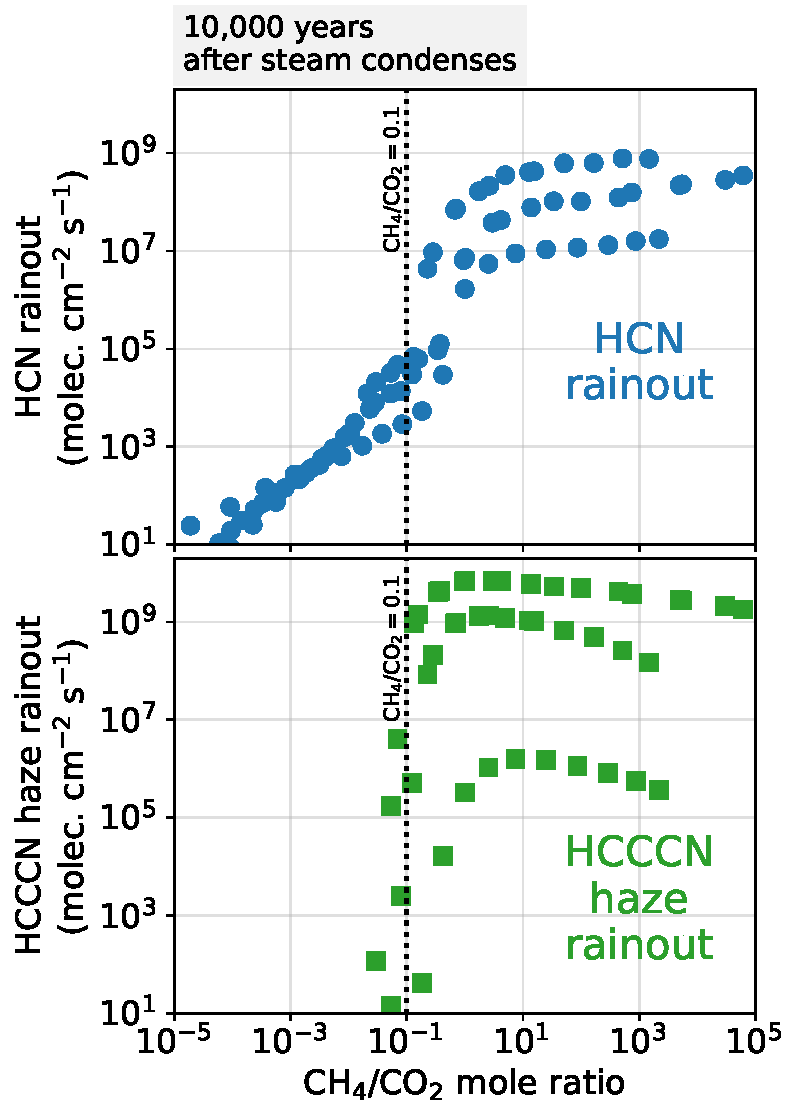
\includegraphics[width=0.5\textwidth]{tex/5impacts/figures/Figure7_5.pdf}
  \caption{HCN rainout and HCCCN haze rainout as a function of the $\mathrm{CH_4}/\mathrm{CO_2}$ mole ratio in all simulated post-impact atmospheres. The figure considers simulations shown in Figure \ref{fig:figure5}, \ref{fig:figure6}, \ref{fig:figure7}, \ref{fig:figure5_citron} and \ref{fig:figure7_citron}. All values are for the atmosphere 10,000 years after steam has condensed to an ocean. The HCN and HCCCN haze production is significantly larger for atmospheres with $\mathrm{CH_4}/\mathrm{CO_2} > 0.1$.}
  \label{fig:figure7_5}
\end{figure}

The impactor mass required to generate an atmosphere with $\mathrm{CH_4}/\mathrm{CO_2} > 0.1$ is uncertain. Our optimistic model, which considers the effect of nickel-catalyzed methane production, requires a $> 4 \times 10^{20}$ kg ($> 570$ km) impactor (Figure \ref{fig:figure7}). The lunar cratering record and abundance of highly siderophile elements Earth's mantle imply that between 4 and 7 such impacts occurred during the Hadean \citep{Marchi_2014, Zahnle_2020}. Our least optimistic model needs a $> 5 \times 10^{21}$ kg ($> 1330$ km) impact to create a post-impact atmosphere with $\mathrm{CH_4}/\mathrm{CO_2} > 0.1$ because it assumes only a fraction of iron delivered to Earth reacts with the ocean to create atmospheric H$_2$ (Appendix Figure \ref{fig:figure5_citron}). The Hadean only experienced 0 to 2 collisions this large \citep{Zahnle_2020}. The precise minimum impactor mass to make an atmosphere with $\mathrm{CH_4}/\mathrm{CO_2} > 0.1$ depends on the importance of atmospheric equilibration with a melt pond (Section \ref{sec:phase1}, and \citet{Itcovitz_2022}), the fraction of impactor iron that reduces the atmosphere, and the effect of Nickel and other surface catalysts on CH$_4$ kinetics.

An additional consideration is that any progress toward the origin of life caused by an impact could be erased by a subsequent impact that sterilizes the planet. For example, suppose a $> 500$ km impact that vaporizes the ocean sterilizes the globe \citep{Citron_2022}. With our most pessimistic calculations for post-impact CH$_4$ generation a $> 1330$ km ($> 5 \times 10^{21}$ kg) impact is required to create an atmosphere that generates significant HCN and HCCCN. In this scenario, the last $> 1330$ km impact favorable for prebiotic chemistry would likely be followed by a $500$ to $1330$ km impact that would destroy any primitive life without rekindling it. Alternatively, our optimistic model for post-impact CH$_4$ generation only requires a $> 4 \times 10^{20}$ kg ($> 570$ km) impact to create an atmosphere with $\mathrm{CH_4}/\mathrm{CO_2} > 0.1$. In this case, the final $> 570$ km impact that might kickstart the origin of life is unlikely to be followed by a slightly smaller $500$ km to $570$ km sterilizing impact.

A caveat to the reasoning in the previous paragraph is that ocean-vaporization may not have sterilized the planet because microbes could have possibly survived in the deep subsurface \citep{Sleep_1989,Grimm_2018}. 

In summary, we suggest that $\mathrm{CH_4}/\mathrm{CO_2} > 0.1$ may be an important threshold for post-impact atmospheres to be conducive to the origin of life because they generate $> 4$ orders of magnitude larger surface HCN concentrations, and are the only modeled atmospheres capable of generating HCCCN. We find that the minimum impactor mass required to create a post-impact atmosphere with $\mathrm{CH_4}/\mathrm{CO_2} > 0.1$ is between $4 \times 10^{20}$ and $5 \times 10^{21}$ kg  ($570$ to $1330$ km). The value is uncertain because we do not know how effectively iron delivered by an impact reduces the atmosphere (Section \ref{sec:phase1}), the importance of atmospheric equilibration with a melt pond (Section \ref{sec:phase1}), and because it is hard to estimate a realistic surface area of nickel catalysts available during the cooling steam atmosphere (Section \ref{sec:phase2}).

\subsection{Model caveats and uncertainties}

Perhaps the most significant caveat to the modeling effort described above is that we did not consider H$_2$ from reactions between a hot post-impact atmosphere and solid, non-melted crust. Section \ref{sec:phase1} explores impact H$_2$ made by two mechanisms: (1) reduction of the atmosphere by impact-derived iron and (2) atmospheric equilibration with a melt pond made by the impact. However, it is also conceivable that while the atmosphere is hot and  steam-rich in the $\sim 10^3$ years following an impact (i.e. Phase 2), water vapor could permeate through and react with the solid crust to produce H$_2$ by a process like serpentinization. Specifically, H$_2$O reduction by FeO in the solid crust could make H$_2$: 

\begin{equation} \label{eq:serp}
  \mathrm{H_2O} + 3 \mathrm{FeO} \rightarrow \mathrm{H_2} + \mathrm{Fe_3O_4}
\end{equation}

In our nominal model (Figure \ref{fig:figure2} and \ref{fig:figure5}), we require a post-impact atmosphere has $> 2 \times 10^3$ H$_2$ mol cm$^{-2}$ (i.e. the equivalent of converting 13\% of Earth's ocean to H$_2$) in order to reach a $\mathrm{CH_4}/\mathrm{CO_2} > 0.1$ and big nitrile production rates. Assuming a crustal FeO content of 8 wt\% \citep{Takahashi_1986}, then $2 \times 10^3$ H$_2$ mol cm$^{-2}$ could be produced by reacting water with FeO in the top $\sim 16$ km of Earth's lithosphere. The feasibility of extensive water-rock H$_2$ generation depends on the permeability of the crust and the pressure gradients driving subsurface fluid circulation. For example, low permeability rocks with slow water circulation may not permit serpentinization of the upper crust within $\sim 10^3$ years while the atmosphere is hot and steam-rich. A comprehensive model is out of the scope of this article, but if attainable, significant water-rock reactions might produce a thick H$_2$ atmosphere after relatively small impacts (e.g. $10^{20}$ kg) which favors a $\mathrm{CH_4}/\mathrm{CO_2} > 0.1$ and significant nitrile generation. 

Another possibility, which we do not investigate in detail, is that atmosphere-crust reactions occur in the immediate aftermath of a giant impact (i.e. Phase 1), rather than over $\sim 10^3$ as previously discussed. A large impact could produce a global ejecta blanket several kilometers thick of mixed hot water and rock. As water was vaporized to form a steam atmosphere, the water and rock slurry could chemically equilibrate, producing H$_2$.

\citet{Zahnle_2020} attempted to account for atmosphere-crust interaction by equilibrating the post-impact steam atmosphere (Phase 2) to a mineral redox buffer. For example, their Figure 5 assumes the atmosphere has a fixed oxygen fugacity set by the FMQ buffer at an assumed 650 K methane quench temperature. The calculation predicts most CO$_2$ is converted to CH$_4$ for impacts as small as $\sim 5 \times 10^{19}$ kg, but \citet{Zahnle_2020} did not determine whether such significant atmosphere-crust interaction is physically plausible.

An additional shortcoming is that our climate model is relatively simple. Throughout the Results section, our climate code assumes an isothermal 200 K stratosphere, a saturated adiabatic troposphere (i.e. relative humidity, $\phi = 1.0$), and ignores clouds. However, many of our simulated post-impact atmospheres contain a hydrocarbon haze which should absorb sunlight and warm the stratosphere \citep{Arney_2016}. Also, in a hydrogen-dominated atmosphere, water vapor has a larger molecular weight compared to the background gas which could inhibit convection \citep{Leconte_2017} and perhaps cause low relative humidities. Furthermore, low-altitude clouds reflect sunlight and should cool a planet while high clouds have a greenhouse warming effect \citep{Goldblatt_2011}.

Figure \ref{fig:figure8} attempts to show the uncertainty in our climate calculations as a function of three free parameters: stratosphere temperature, relative humidity, and low-altitude clouds which we crudely approximate by varying the surface albedo. The calculation uses the composition of the atmosphere after a $5 \times 10^{20}$ kg impact in Figure \ref{fig:figure7} immediately after the steam atmosphere has condensed to an ocean. Our nominal climate parameters ($T_\mathrm{strat} = 200$ K, $\phi = 1$, $A_s = 0.2$) predict a 361 K surface temperature. A warm stratosphere caused by hydrocarbon UV absorption and high albedo surface clouds might cause the surface to be $\sim 30$ K colder than our nominal model, assuming water vapor is saturated. On the other hand, low relative humidities, which might be favored in convection-inhibited H$_2$ dominated atmospheres, flatten the troposphere adiabat which warms the surface \citep{Leconte_2017}. While Figure \ref{fig:figure8} gives a sense for the possible uncertainty in our climate calculations, it does not self-consistently simulate haze, relative humidity and clouds feedbacks. A more comprehensive model is required to resolve these nuances.

\begin{figure}
  \centering
  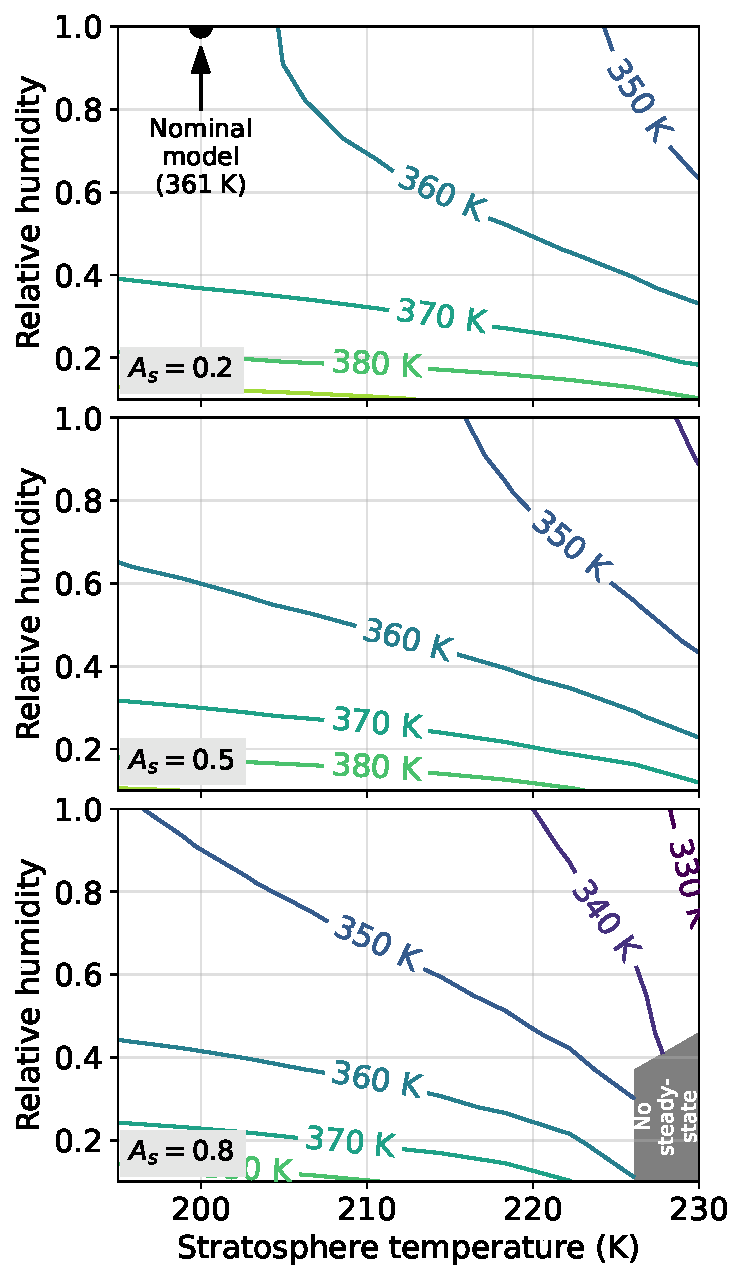
\includegraphics[width=0.5\textwidth]{tex/5impacts/figures/Figure8.pdf}
  \caption{Surface temperature of a post-impact atmosphere as a function of stratosphere temperature, relative humidity, and surface clouds which we crudely approximate with the surface albedo ($A_b$). The atmosphere has 5.9 mol cm$^{-2}$ CO$_2$, 5.6 mol cm$^{-2}$ CH$_4$, 36 mol cm$^{-2}$ N$_2$, 557 mol cm$^{-2}$ H$_2$, 0.01 mol cm$^{-2}$ CO, and a liquid water ocean at the surface. This is the same composition of the atmosphere after a $5 \times 10^{20}$ kg impact in Figure \ref{fig:figure7} once steam has condensed to an ocean. The gray shaded region labeled ``no steady-state'' has no steady-state climate solutions that balance incoming shortwave and outgoing longwave energy. Uncertainties in our assumed stratosphere temperature, relative humidity and the effects of low-altitude clouds predict surface temperatures from $\sim 330$ K to $\sim 390$ K with a nominal value of 361 K.}
  \label{fig:figure8}
\end{figure}

Moreover, our photochemical model does not include ion chemistry, which is likely a reasonable simplification because ions are not important for HCN or HCCCN formation on Titan \citep{Loison_2015}. Only some heavy hydrocarbons, like benzene (C$_6$H$_6$), rely on coupled neutral-ion chemistry to explain their observed abundances in Titan's atmosphere \citep{Horst_2017}.

\section{Conclusions}

We use atmospheric models to investigate the production of prebiotic feedstock molecules in impact-generated reducing atmospheres on the Hadean Earth, updating simpler calculations made by \citet{Zahnle_2020}. We find that massive asteroid impacts can generate temporary H$_2$-, CH$_4$- and NH$_3$-rich atmospheres, which photochemically generate HCN and HCCCN for the duration of hydrogen escape to space ($10^5$ to $10^7$ years). The production of nitriles increases dramatically for haze-rich atmospheres that have mole ratios of $\mathrm{CH_4}/\mathrm{CO_2} > 0.1$. In these cases, HCN can rain out onto land surfaces at a rate of $\sim 10^9$ molecules cm$^{-2}$ s$^{-1}$, and HCCCN incorporated in haze rains out at a similar rate. Atmospheres with $\mathrm{CH_4}/\mathrm{CO_2} < 0.1$ produce 3 to 4 orders of magnitude less HCN, and generate negligible HCCCN. The impactor mass required to create an atmosphere with $\mathrm{CH_4}/\mathrm{CO_2} > 0.1$ is uncertain and depends on how efficiently atmosphere-iron, atmosphere-melt and atmosphere-crust reactions generate H$_2$ and the surface area of nickel catalysts exposed to the cooling steam atmosphere. In an optimistic modeling scenario a $> 4 \times 10^{20}$ kg ($> 570$ km) impactor is sufficient, while in our least optimistic scenario a $> 5 \times 10^{21}$ kg ($> 1330$ km) impactor is required. 

We find that post-impact atmospheres that generate significant prebiotic molecules have $> 360$ K surface temperatures caused by a H$_2$-H$_2$ greenhouse which may be too hot for prebiotic chemistry, although the temperature may be cooler if reflective clouds occur. An alternative is that HCN and HCCCN generated in post-impact atmosphere are stockpiled. Cyanide can plausibly be stockpiled and concentrated in ferrocyanide salts and cyanoacetylene could be captured by byproducts of adenine synthesis into imidazole-based crystals \citep{Ritson_2022}. HCN and HCCCN can be used to create nucleotide precursors to RNA millions of years after the impact, once the H$_2$ has escaped to space, and the atmosphere has cooled to a more temperate state.

Nominally, the Hadean Earth appears to have experienced several impacts that would have produced an atmosphere that made significant prebiotic feedstock molecules. Like Earth, all rocky exoplanets accreted from impacts. Consequently, impact-induced reducing atmospheres may be a common planetary processes that provides windows of opportunity for the origin of exoplanet life.

\section{Chapter Appendix} \label{sec:impacts_appendix}

\begin{figure}
  \centering
  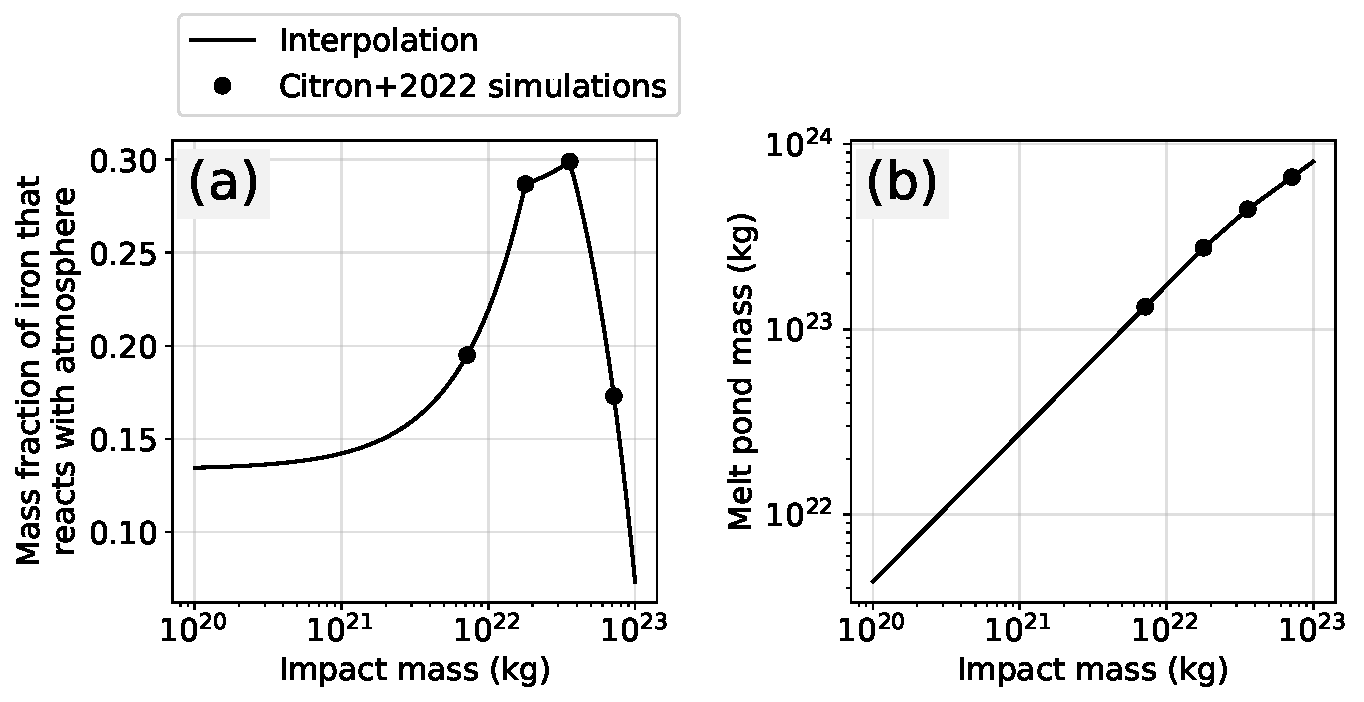
\includegraphics[width=0.9\textwidth]{tex/5impacts/figures/supplement/citron_interpolations.pdf}
  \caption{Interpolation and extrapolation of the \citet{Citron_2022} SPH simulations of impacts that collide with Earth at a $45^\circ$ angle and with a velocity of twice Earth's escape velocity. (a) is the mass fraction of iron that reacts with the atmosphere and (b) is the mass of the melt pool produced by an impact.  These interpolations are relevant to Figure \ref{fig:melt_reaction_sup} in the main text, and Appendix Figures \ref{fig:figure2_citron}, \ref{fig:figure3_citron}, \ref{fig:figure5_citron}, and \ref{fig:figure7_citron}.}
  \label{fig:citron_interpolations}
\end{figure}

\begin{figure}
  \centering
  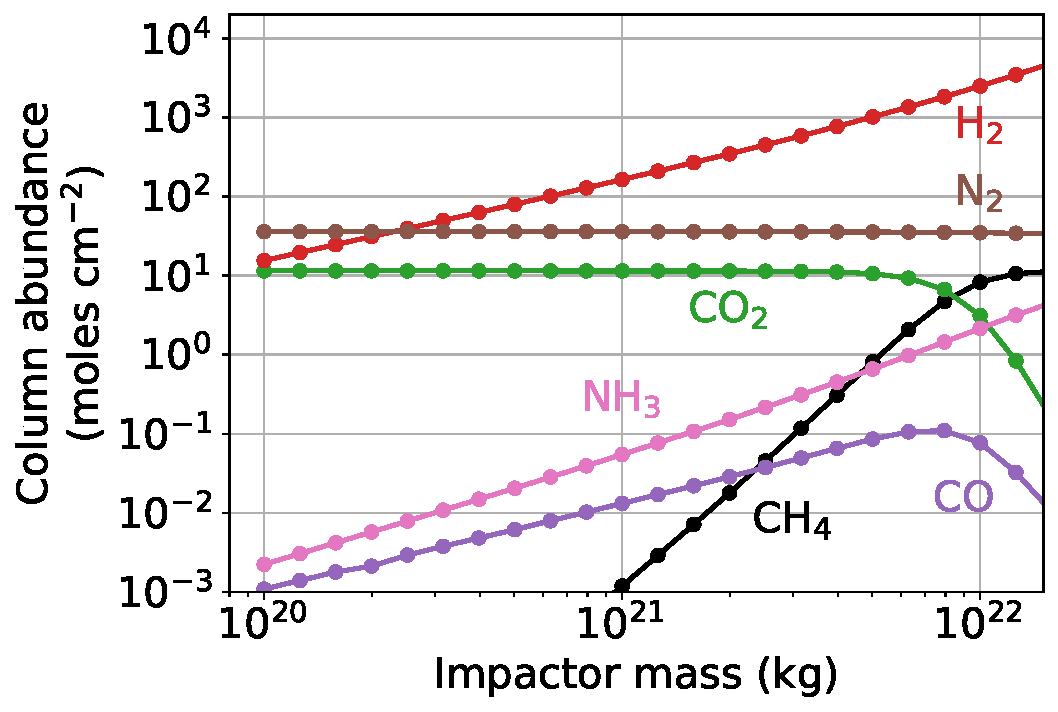
\includegraphics[width=0.65\textwidth]{tex/5impacts/figures/supplement/Figure2_Citron.pdf}
  \caption{Identical to Figure \ref{fig:figure2} in the main text, but instead assumes post-impact H$_2$ generation if governed by ``Model 1B'' described in Figure \ref{fig:melt_reaction_sup}.}
  \label{fig:figure2_citron}
\end{figure}

\begin{figure}
  \centering
  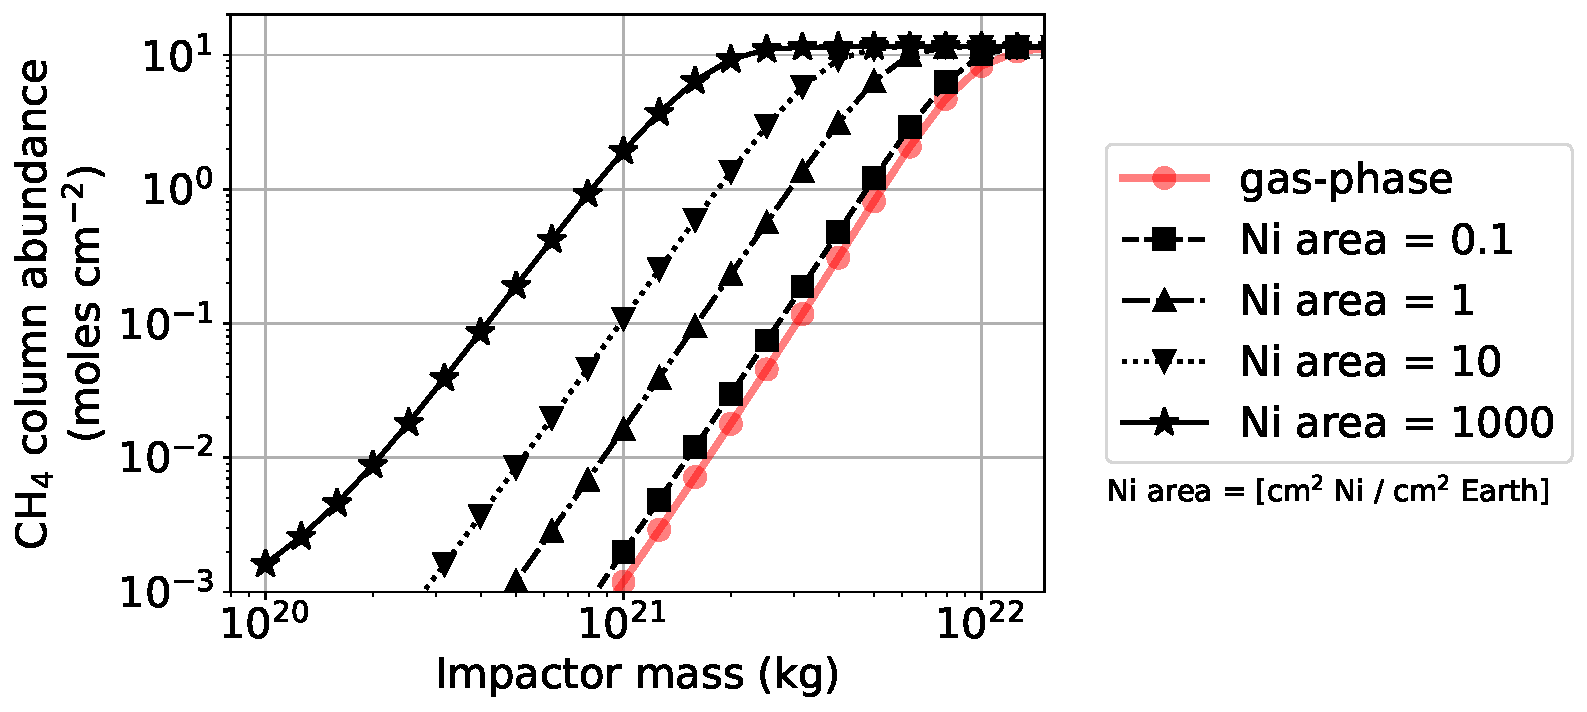
\includegraphics[width=0.8\textwidth]{tex/5impacts/figures/supplement/Figure3_Citron.pdf}
  \caption{Identical to Figure \ref{fig:figure3} in the main text, but instead assumes post-impact H$_2$ generation if governed by ``Model 1B'' described in Figure \ref{fig:melt_reaction_sup}.}
  \label{fig:figure3_citron}
\end{figure}

\begin{figure}
  \centering
  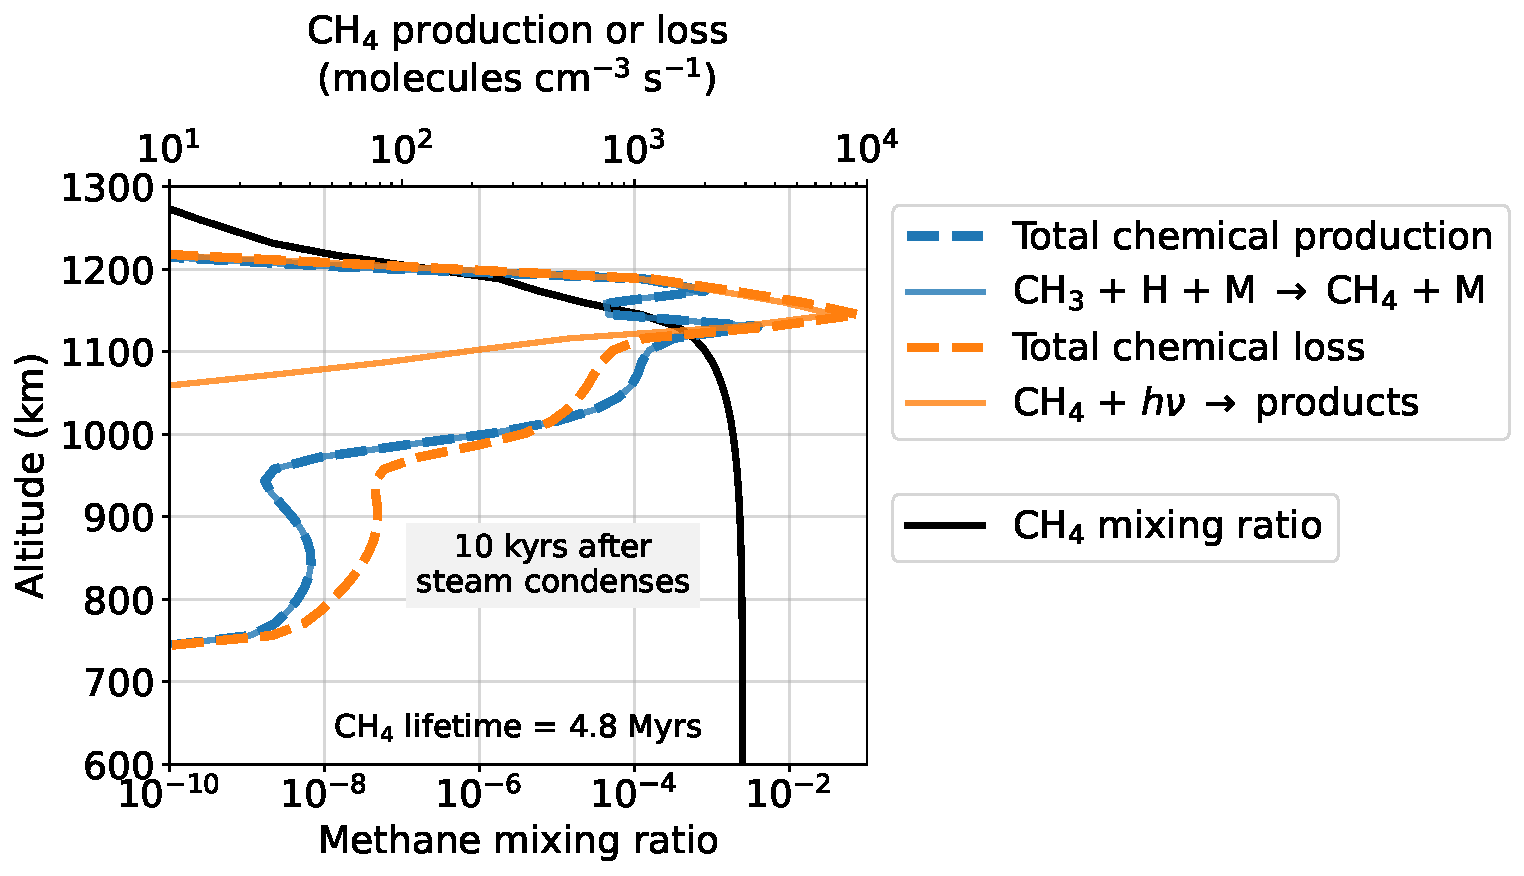
\includegraphics[width=0.8\textwidth]{tex/5impacts/figures/supplement/CH4_prod_and_loss.pdf}
  \caption{The methane photochemical lifetime in post-impact atmospheres. The plot shows the CH$_4$ mixing ratio and production and loss as a function of altitude 10,000 years after the steam atmosphere has condensed to an ocean following the $1.58 \times 10^{21}$ kg impact described in Figure \ref{fig:figure4}. CH$_4$ is primarily destroyed by photolysis, but reforms efficiently in the H$_2$ rich atmosphere from $\mathrm{CH_3} + \mathrm{H} + \mathrm{M} \rightarrow \mathrm{CH_4} + \mathrm{M}$. The result is a 4.8 million year CH$_4$ photochemical lifetime. CH$_4$ only persists in the atmosphere for about one million years because H$_2$ escapes to space in this amount of time which inhibits CH$_4$ recombination.}
  \label{fig:ch4_prod_loss}
\end{figure}

\begin{figure}
  \centering
  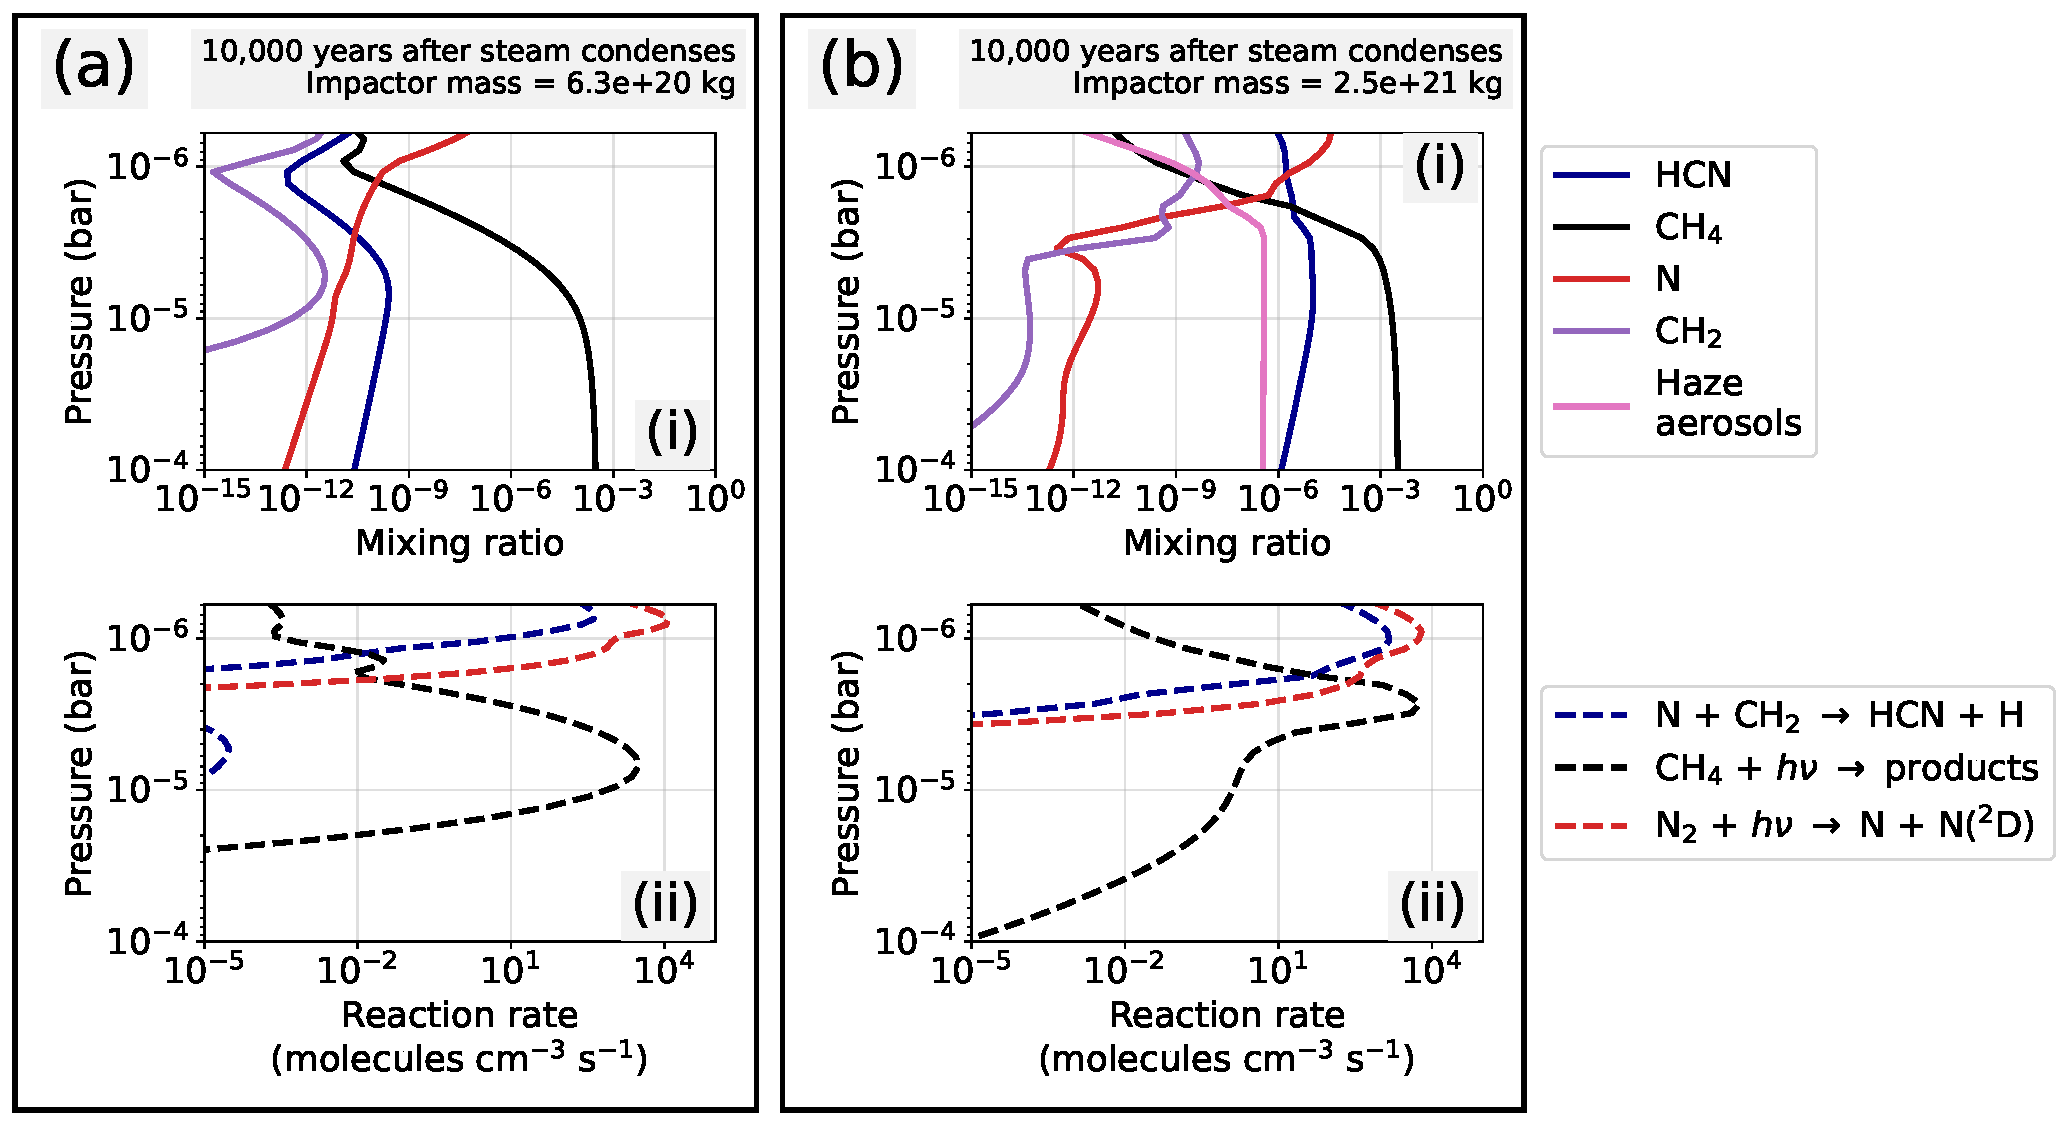
\includegraphics[width=1.0\textwidth]{tex/5impacts/figures/supplement/CH4_N_HCN.pdf}
  \caption{HCN production and precursor species after a (a) $6.3 \times 10^{20}$ kg and (b) $2.5 \times 10^{21}$ kg impactor. In both (a) and (b) panels (i) shows mixing ratios, while (ii) shows photolysis and reaction rates. Panel (b) contains haze aerosols which cause CH$_4$ photolysis to be higher in the atmosphere compared to panel (a). High altitude CH$_4$ photolysis, closer to N$_2$ photolysis, promotes HCN production because photolysis produced can more readily combine to make cyanides.}
  \label{fig:ch4_n_hcn}
\end{figure}

\begin{figure}
  \centering
  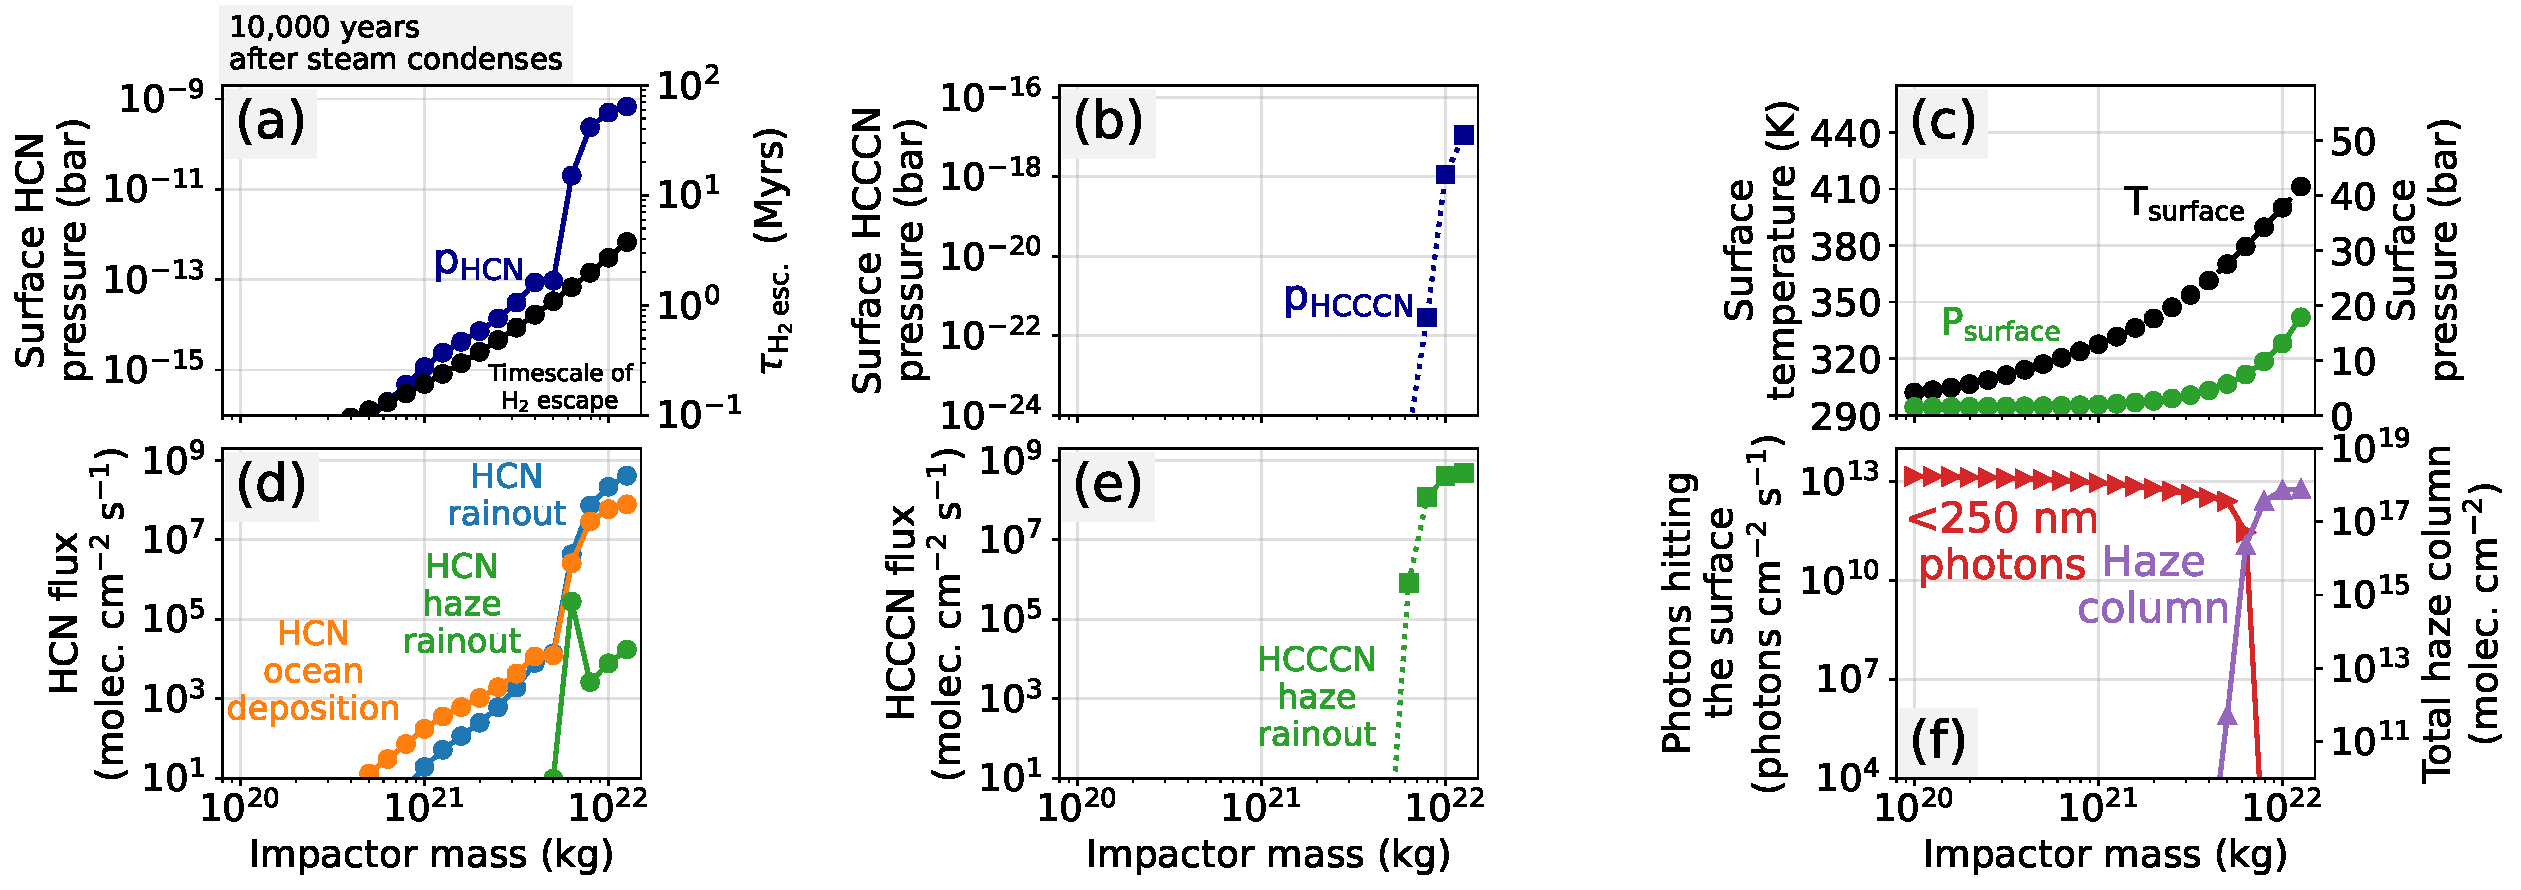
\includegraphics[width=1.0\textwidth]{tex/5impacts/figures/supplement/Figure5_Citron.pdf}
  \caption{Identical to Figure \ref{fig:figure5} in the main text, but instead assumes post-impact H$_2$ generation if governed by ``Model 1B'' described in Figure \ref{fig:melt_reaction_sup}.}
  \label{fig:figure5_citron}
\end{figure}

\begin{figure}
  \centering
  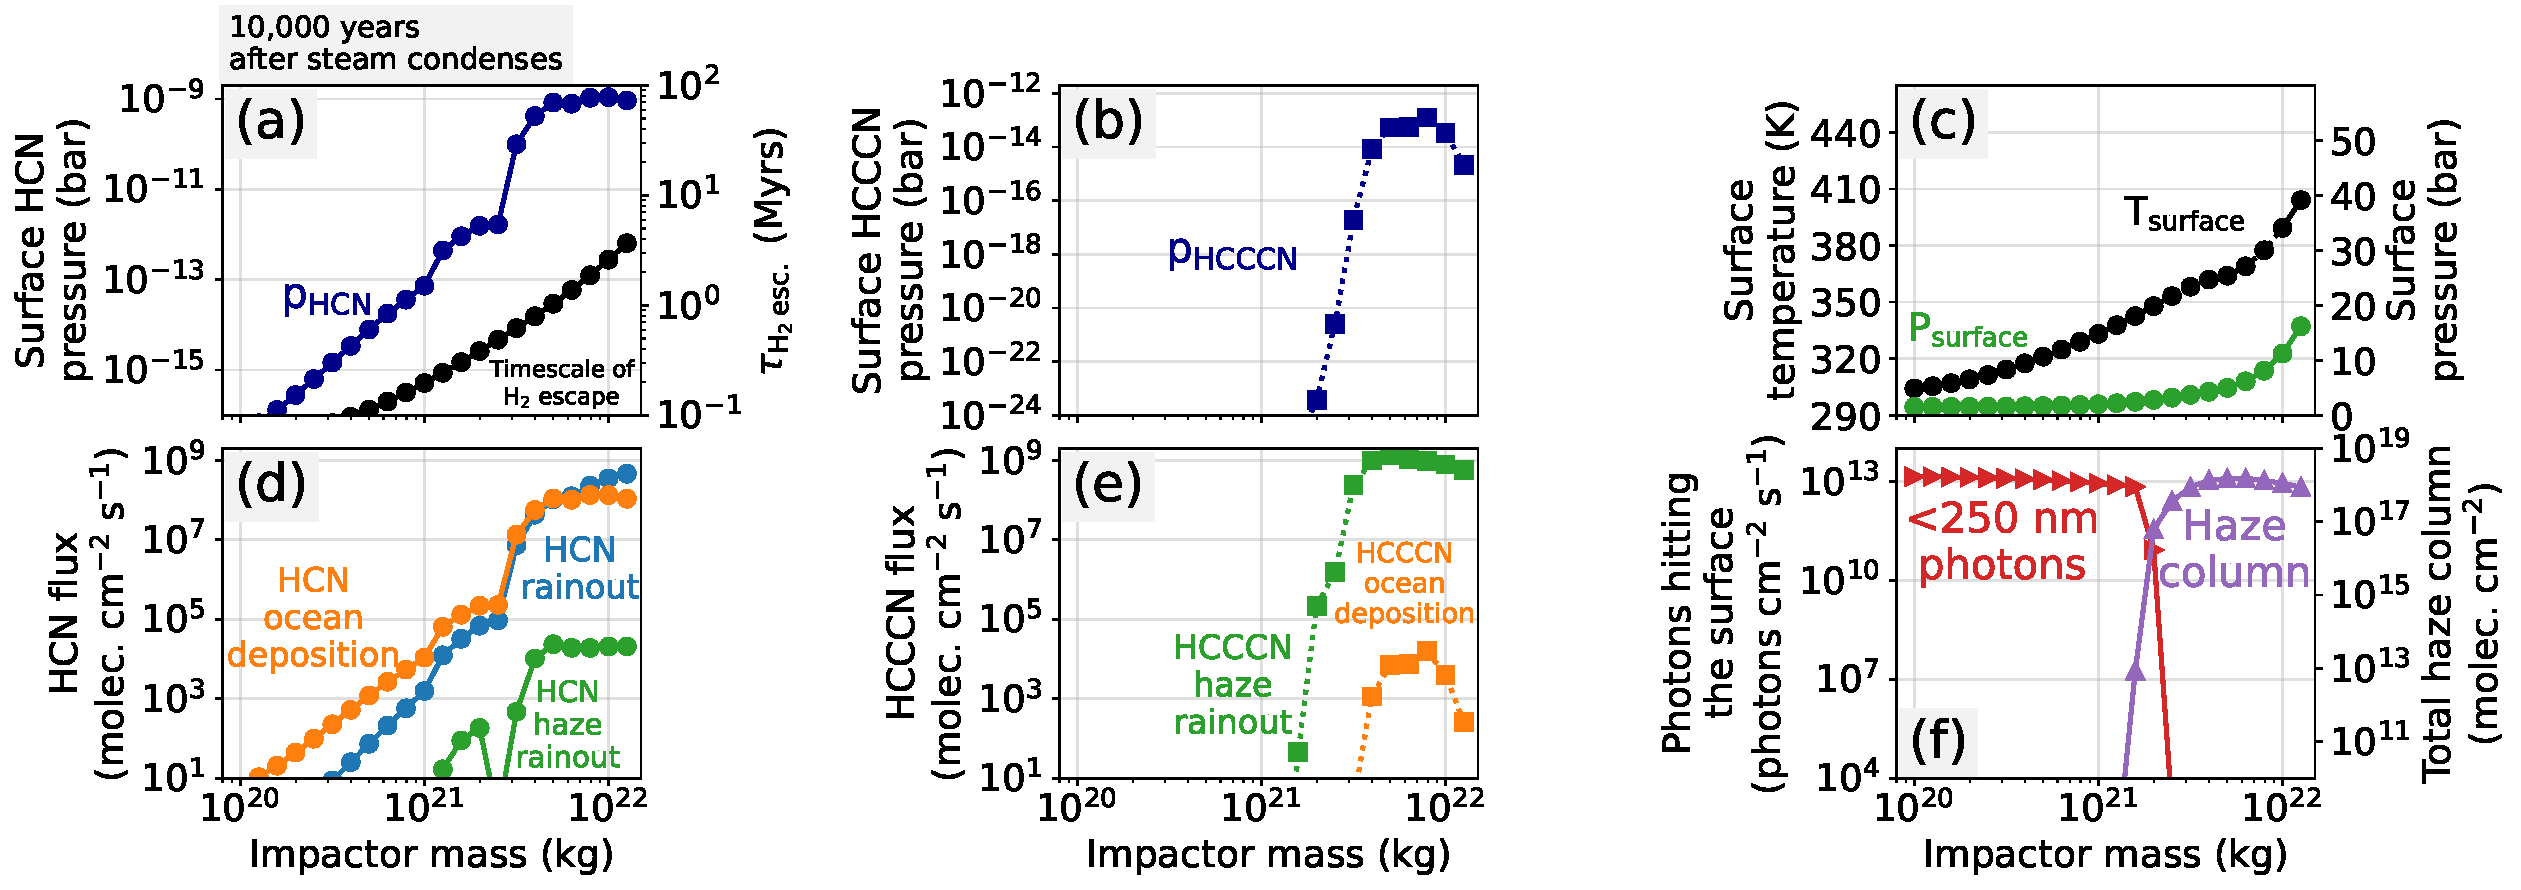
\includegraphics[width=1.0\textwidth]{tex/5impacts/figures/supplement/Figure7_Citron.pdf}
  \caption{Identical to Figure \ref{fig:figure7} in the main text, but instead assumes post-impact H$_2$ generation if governed by ``Model 1B'' described in Figure \ref{fig:melt_reaction_sup}.}
  \label{fig:figure7_citron}
\end{figure}

\begin{figure}
  \centering
  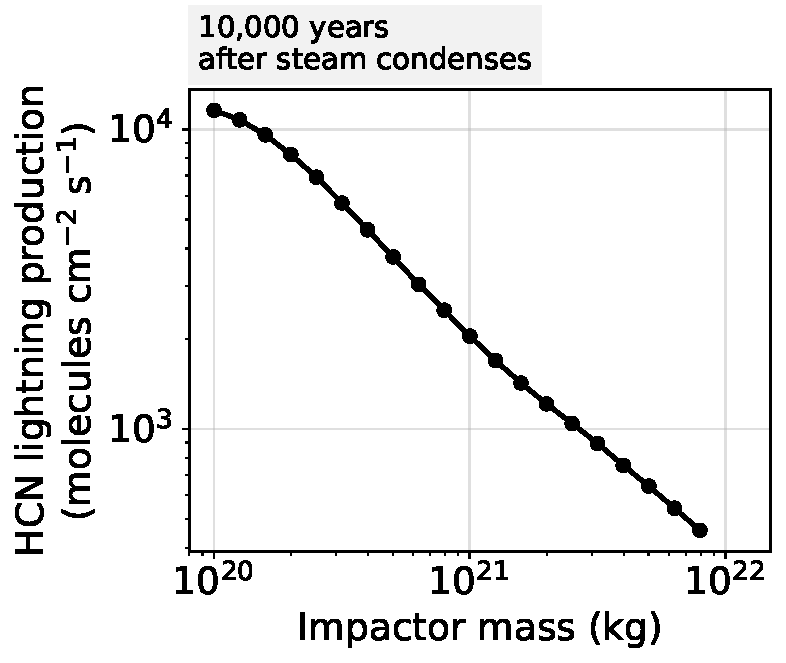
\includegraphics[width=0.5\textwidth]{tex/5impacts/figures/supplement/Figure5_lightning.pdf}
  \caption{HCN production from lighting for the same simulations and time-period shown in Figure \ref{fig:figure5}. The calculations use methods described in \citet{Chameides_1981} assuming modern Earth's lightning dissipation rate ($9.8 \times 10^{-9}$ J cm$^{-2}$ s$^{-1}$), and a 2250 K HCN freeze-out temperature. HCN production from lightning is small compared to what is achievable with photochemistry.}
  \label{fig:figure5_lightning}
\end{figure}

\subsection{H\textsubscript{2} generation from iron and molten crust} \label{sec:phase1_appendix}

Here, we describe our model for atmospheric H$_2$ generation in the days to months following a massive asteroid impact (Phase 1 in Figure \ref{fig:impact_diagram}). All our simulations assume a pre-impact atmosphere containing CO$_2$, N$_2$, and ocean water. First, we assume that half of the impactor's kinetic energy heats the atmosphere and ocean water to $\sim 2000$ K. We assume the atmosphere is heated to $\sim 2000$ K because this is roughly the evaporation temperature of silicates. For our assumed impact velocity of $20.7$ km s$^{-1}$, all impactor masses that we consider in the main text ($10^{20}$ to $10^{22}$ kg) have kinetic energies $> 2 \times 10^{28}$ joules delivering $> 10^{28}$ joules to the atmosphere which is larger than the $5 \times 10^{27}$ joules required to vaporize an ocean \citep{Sleep_1989}. 

Next, our model assumes each mole of iron delivered reacts with the atmosphere and removes one mole of oxygen. The moles cm$^{-2}$ of iron delivered to the atmosphere is

\begin{equation}
  N_\mathrm{Fe,atmos} = \frac{X_\mathrm{Fe,atmos} X_\mathrm{Fe,imp} M_\mathrm{imp}}{\mu_\mathrm{Fe} A_\oplus}
\end{equation}
Here, $M_\mathrm{imp}$ is the mass of the impact in grams, $X_\mathrm{Fe,imp}$ is the iron mass fraction of the impact, $X_\mathrm{Fe,atmos}$ is the fraction of the impactor iron that reacts with the atmosphere, $\mu_\mathrm{Fe}$ is the molar weight of iron, and $A_\oplus$ is the area of Earth in cm$^2$. Following \citet{Zahnle_2020} we take $X_\mathrm{Fe,imp} = 0.33$. In main text, we assume $X_\mathrm{Fe,atmos} = 1$ (e.g. ``Model 1A'' in Figure \ref{fig:melt_reaction_sup}), while the Appendix contains calculations with $X_\mathrm{Fe,atmos} = 0.15$ to $0.3$ based on extrapolations of the \citet{Citron_2022} SPH impact simulations for $45^{\circ}$ impactors traveling at 20.7 km s$^{-1}$ (e.g. ``Model 1B'' in Figure \ref{fig:melt_reaction_sup}). To approximate equilibration between the delivered iron and the atmosphere, we simply remove $N_\mathrm{Fe,atmos}$ of O from the atmosphere.

Our model also optionally considers reactions between the atmosphere and a melt pond generated by the impact. Our approach is similar to the one described in \citet{Itcovitz_2022}. We estimate the total mass of the melt pond ($M_\mathrm{melt}$) by interpolating SPH impact simulations from \citet{Citron_2022} for a $45^{\circ}$ impact angle. The smallest impact they consider is $7 \times 10^{21}$ kg, so we extrapolate their results down to $10^{20}$ kg. We additionally take the melted crust to be basaltic in composition except with variable initial amounts of ferric and ferrous iron. Effectively, this means that the initial oxygen fugacity of the melted crust is a free parameter because iron redox state is related to oxygen fugacity through the equilibrium reaction,

\begin{equation} 
  \label{eq:kress_carmichael_1}
  0.5 \mathrm{O_2} + 2 \mathrm{FeO} \leftrightarrow \mathrm{Fe_2O_3}
\end{equation}
We assume the oxygen atoms can flow from the atmosphere into the melt (or vice-versa) in order to bring Reaction \ref{eq:kress_carmichael_1} to an equilibrium state defined by \citet{Kress_1991} thermodynamic data. Our model also considers H$_2$O gas dissolution in the melt using the Equation (19) solubility relation in \citet{Itcovitz_2022}.

Finally, given a heated post-impact atmosphere that has been reduced by impactor iron and, optionally, in contact with an melt pool, we compute thermodynamic equilibrium of the atmosphere-melt system at $1900$ K. We choose 1900 K because any impact-produced silicate vapors should have condensed and rained out of the atmosphere, and the melt pool should have not yet solidified \citep{Itcovitz_2022}. To find an equilibrium state, we first compute an equilibrium composition for the atmosphere alone using the equilibrium solver in the Cantera chemical engineering package \citep{Goodwin_2022} with our thermodynamic data (Appendix \ref{sec:photochem_reactions}). Next, to equilibrate the atmosphere-melt system, we perform a zero-dimensional kinetics integration for 1000 years at constant temperature and pressure with our reaction network (Appendix \ref{sec:photochem_reactions}). All reactions in our network are reversible thermodynamically, therefore integrating the kinetics forward in time should ultimately reach a state of thermodynamic equilibrium. Our integration includes additional reactions representing Reaction \ref{eq:kress_carmichael_1} and H$_2$O dissolution in the melt. We arbitrarily choose forward reaction rates of $10^{-10}$ s$^{-1}$ for both reactions, then reverse the rates using the \citet{Kress_1991} equilibrium constant, and the Equation (19) solubility relation in \citet{Itcovitz_2022}. Overall, our approach finds a chemical equilibrium state between the atmosphere and the melt pond, and therefore an estimation of the amount of H$_2$ generated from atmosphere-iron and atmosphere-melt reactions.

Our code for solving melt-atmosphere equilibrium is available at the following Zenodo link: \url{https://doi.org/10.5281/zenodo.7802966}.

\subsection{Kinetics model of a cooling steam atmosphere} \label{sec:kinetics_climate}

We simulate the chemistry of a cooling post-impact atmosphere using a zero-dimensional kinetics-climate model. We assume the atmosphere's composition, pressure, and temperature are homogeneous in all directions, and has a vertical extent of one atmospheric scale height ($H_a$). For these assumptions, the following system of ordinary differential equations govern our model:

\begin{equation} \label{eq:prod_loss}
  \frac{\partial N_i}{\partial t} = \frac{H_a}{N_a} (P_i - L_i) + \frac{A_c}{N_a} (P_{i,\text{surf}} - L_{i,\text{surf}})
\end{equation}
\begin{equation} \label{eq:temp}
  \frac{\partial T_s}{\partial t} = -\frac{1}{\rho c_p} \left(\frac{F_\text{net}}{H_a}\right) - \frac{1}{\rho c_p}\left(\frac{d M_\mathrm{H_2O}}{dt} \frac{l_\mathrm{H_2O}}{A_\oplus H_a}\right) 
\end{equation}

All variables and units are in Table \ref{tab:5impacts_variables}. In Equation \eqref{eq:prod_loss}, $N_i$ is the column abundance of species $i$ in mole cm$^{-2}$, which changes because of gas-phase chemical reactions (production rate $P_i$ and loss rate $L_i$) and reactions occurring on surfaces ($P_{i,\text{surf}}$ and $L_{i,\text{surf}}$). In Equation \eqref{eq:temp}, $T$ is surface temperature, which changes because of energy radiated to space ($F_\text{net}$), and because of latent heat from H$_2$O condensation ($\frac{d M_\mathrm{H_2O}}{dt}$), where $M_\mathrm{H_2O}$ is the mass of H$_2$O in the atmosphere. We approximate the energy radiated to space in ergs cm$^{-2}$ s$^{-1}$ from a steam-dominated atmosphere with the following parameterization:

\begin{equation}
  F_\text{net} = 8.3 \times 10^4 + 1000 \max(T_s - 1750,0)
\end{equation}
This parameterization fits calculations from our radiative transfer model (see Appendix \ref{sec:clima}), which uses the a solar spectrum at 4.0 Ga derived from methods described in \citet{Claire_2012}. 

We can rewrite Equation \eqref{eq:temp}, replacing $\rho H_a$ using the ideal gas law and the definition of atmospheric scale height,

\begin{equation}
  \rho H_a = \frac{p \bar\mu}{N_a k T} \frac{N_a k T}{\bar\mu g} = \frac{p}{g}
\end{equation}
Here, $p$ is the total atmospheric pressure in dynes cm$^{-2}$, $g$ is gravitational acceleration in cm s$^{-2}$, $k$ is the Boltzmann constant, $\bar\mu$ is the mean molecular weight in g mol$^{-1}$, and $N_a$ is Avogadro's number. Therefore,

\begin{equation} \label{eq:temp0}
  \frac{\partial T_s}{\partial t} = -\frac{g}{p c_p} F_\text{net} - \frac{g}{p c_p}\left(\frac{d M_\mathrm{H_2O}}{dt} \frac{l_\mathrm{H_2O}}{A_\oplus}\right) 
\end{equation}

Next, we must derive an expression for the steam condensation rate ($d M_\mathrm{H_2O}/dt$) in terms of known variables. Working in CGS units, the total pressure of the atmosphere is given by its gravitational force divided by Earth's surface area ($5.1 \times 10^{18}$ cm$^2$):

\begin{equation}
 p = \frac{Mg}{A_\oplus}
\end{equation}
Here, $M$ is the mass of the atmosphere in grams. We are considering steam-dominated atmospheres, therefore, the mass and pressure in the above relation is approximately equal to the mass of atmospheric H$_2$O and the H$_2$O partial pressure.

\begin{align}
  p_\mathrm{H_2O} &\approx \frac{M_\mathrm{H_2O}g}{A_\oplus} \\
  M_\mathrm{H_2O} &\approx \frac{p_\mathrm{H_2O}A_\oplus}{g} \label{eq:atmos_pressure}
\end{align}
Taking a time derivative of Equation \eqref{eq:atmos_pressure} yields

\begin{equation}
  \frac{d M_\mathrm{H_2O}}{dt} \approx \frac{A_\oplus}{g} \frac{d p_\mathrm{H_2O}}{dt} \label{eq:conden}
\end{equation}
We assume that the only processes changing the H$_2$O mass in the atmosphere is condensation, which occurs in our model when steam becomes saturated. We further assume that the H$_2$O partial pressure is fixed at saturation once steam condensation begins. We approximate the saturation vapor pressure of H$_2$O, $p_\mathrm{H_2O}^\text{sat}$, using the Clausius-Clapeyron equation, assuming a temperature-independent latent heat, $l_\mathrm{H_2O}$,

\begin{equation}
  p_\mathrm{H_2O}^\text{sat} = p_0 \exp\left(\frac{l_\mathrm{H_2O} \mu_\mathrm{H_2O}}{R}\left( \frac{1}{T_0} - \frac{1}{T}  \right)\right) \label{eq:sat_press}
\end{equation}
$p_0$ and $T_0$ are reference pressures and temperatures, respectively. Taking a time derivative of Equation \eqref{eq:sat_press} yields

\begin{equation}
  \frac{dp_\mathrm{H_2O}^\text{sat}}{dt} = \left(\frac{l_\mathrm{H_2O} \mu_\mathrm{H_2O}}{RT^2}\right) \frac{dT_s}{dt} p_\mathrm{H_2O}^\text{sat} \label{eq:sat_press_deriv}
\end{equation}
Substituting Equation \eqref{eq:sat_press_deriv} into Equation \eqref{eq:conden} gives

\begin{equation}
  \frac{d M_\mathrm{H_2O}}{dt} = \frac{A_\oplus}{g} \left(\frac{l_\mathrm{H_2O} \mu_\mathrm{H_2O}}{RT^2}\right) \frac{dT_s}{dt} p_\mathrm{H_2O}^\text{sat} \label{eq:conden2}
\end{equation}
Finally, we can substitute Equation \eqref{eq:conden2} into Equation \eqref{eq:temp0} and rearrange to solve for $dT/dt$. The result below gives the rate of change of temperature when the steam is too hot to condense ($p_\mathrm{H_2O} > p_\mathrm{H_2O}^\text{sat}$), and when the steam is condensing ($p_\mathrm{H_2O} = p_\mathrm{H_2O}^\text{sat}$).
\begin{equation} \label{eq:temp1}
  \frac{d T_s}{d t} = 
  \begin{cases} 
    -\frac{g}{p c_p} F_\text{net} & p_\mathrm{H_2O} > p_\mathrm{H_2O}^\text{sat} \\
    -\frac{g}{p c_p} F_\text{net}\left( 1 + \frac{l_\mathrm{H_2O}^2 \mu_\mathrm{H_2O} p_\mathrm{H_2O}^\text{sat}}{p c_p R T^2} \right)^{-1} & p_\mathrm{H_2O} = p_\mathrm{H_2O}^\text{sat}
 \end{cases}
\end{equation} 

Equations \eqref{eq:prod_loss} and \eqref{eq:temp1} are a system of ordinary differential equations, which we approximately solve over time using the CVODE BDF method developed by Sundials Computing \citep{Hindmarsh_2005}. Additionally, for either gas-phase or surface reactions, we make use of the Cantera software library \citep{Goodwin_2022} to compute chemical production and destruction rates. Our code for solving the equations derived in this section is available at the following Zenodo link: \url{https://doi.org/10.5281/zenodo.7802966}.

\begin{spacing}{1.0}
\begin{center}
  \begin{tabularx}{\linewidth}{p{0.15\linewidth} | p{0.55\linewidth} | p{0.3\linewidth}} \caption{Variables} \label{tab:5impacts_variables} \\
  \hline \hline
  Variable & Definition & Units \\
  \hline
  $f_{i}$ & Mixing ratio of species $i$ & dimensionless 
  \\
  $n_{i}$ & Number density of species $i$ & molecules cm$^{-3}$ 
  \\
  $n$ & Total number density & molecules cm$^{-3}$ 
  \\
  $N_{i}$ & Column abundance of species $i$ & mol cm$^{-2}$ 
  \\
  $N$ & Total column abundance & mol cm$^{-2}$ 
  \\
  $\rho$ & Density of the atmosphere & g cm$^{-3}$ 
  \\
  $c_p$ & Specific heat capacity of the atmosphere & erg g$^{-1}$ K$^{-1}$
  \\
  $F_\text{net}$ & Net radiative energy leaving the atmosphere & erg cm$^{-2}$ s$^{-1}$
  \\
  $z$ & Altitude & cm 
  \\
  $t$ & Time & seconds 
  \\
  $P_{i}$ & Total chemical production of species $i$ & molecules cm$^{-3}$ s$^{-1}$ 
  \\
  $L_{i}$ & Total chemical loss of species $i$ & molecules cm$^{-3}$ s$^{-1}$ 
  \\
  $P_{i,\text{surf}}$ & Total chemical production of species $i$ from surface reactions & molecules
  cm$^{-2}$ s$^{-1}$ 
  \\
  $L_{i,\text{surf}}$ & Total chemical loss of species $i$ from surface reactions & molecules
  cm$^{-2}$ s$^{-1}$ 
  \\
  $R_{\text{i, rainout}}$ & Production and loss of species $i$ from rainout & molecules cm$^{-3}$ s$^{-1}$
  \\
  $Q_{i\text{, cond}}$ & Production and loss of species $i$ from condensation and evaporation & molecules cm$^{-3}$ s$^{-1}$
  \\
  $\Phi_{i}$ & Vertical flux of species $i$ & molecules cm$^{-2}$ s$^{-1}$ 
  \\
  $K_{zz}$ & Eddy diffusion coefficient & cm$^{-2}$ s$^{-1}$ 
  \\
  $D_{i}$ & Molecular diffusion coefficient & cm$^{-2}$ s$^{-1}$ 
  \\
  $H_{i}$ & $= N_{a}\text{kT}\text{/}\mu_{i}g$, The scale heights of species $i$ & cm 
  \\
  $H_{a}$ & $= N_{a}\text{kT}\text{/}\overline{\mu}g$, The average scale height. & cm 
  \\
  $N_{a}$ & Avogadro's number & molecules mol$^{-1}$ 
  \\
  $k$ & Boltzmann's constant & erg K$^{-1}$ 
  \\
  $R$ & Gas constant & erg mol$^{-1}$ K$^{-1}$ 
  \\
  $\mu$ & Molar mass. $\overline{\mu}$ is mean molar mass of the atmosphere, and $\mu_{i}$ is the molar mass of species $i$ & g mol$^{-1}$ 
  \\
  $A_c$ & Catalyst surface area per atmospheric column & cm$^2$ catalyst / cm$^2$ Earth
  \\
  $l_\mathrm{H_2O}$ & Latent heat of H$_2$O condensation & erg g$^{-1}$ 
  \\
  $A_\oplus$ & Area of Earth's surface & cm$^2$
  \\
  $\phi$ & Relative humidity & dimensionless
  \\
  $A_s$ & Optical surface albedo & dimensionless
  \\
  $p$ & Atmospheric pressure. $p_\mathrm{i}$ is the partial pressure of species $i$. & dynes cm$^{-2}$ 
  \\
  $M$ & Mass of the atmosphere. $M_\mathrm{i}$ is the mass of species $i$. $M_\mathrm{imp}$ is the mass of an impactor. & g
  \\
  $g$ & Gravitational acceleration & cm s$^{-2}$ 
  \\
  $\alpha_{\text{Ti}}$ & Thermal diffusion coefficient of species $i$. We neglect this term ($\alpha_{\text{Ti}} = 0$) & dimensionless
  \\
  $T$ & Temperature. $T_s$ is the surface temperature. & K 
  \\
  \hline
  \end{tabularx}
\end{center}
\end{spacing}

\subsection{The \emph{Photochem} model} \label{sec:photochem}

To simulate the photochemistry of post-impact reducing atmospheres, we developed a photochemical model called \emph{Photochem}. The model is a re-written and vastly updated version of \emph{PhotochemPy} \citep{Wogan_2022}. \emph{Photochem} is written in modern Fortran and C, with a Python interface made possible by Cython \citep{Behnel_2010}. This article uses \emph{Photochem} version v0.3.14 archived in the following Zenodo repository: \url{https://doi.org/10.5281/zenodo.7802921}.

The following sections briefly describe the fundamental model equations solved by \emph{Photochem}, our chemical network, and validates the model against observations of Earth and Titan.

\subsubsection{Model equations}

We begin our derivation of the equations governing \emph{Photochem} with modified versions of Equations B.1, B.2 and B.29 in \citet{Catling_2017}:

\begin{gather}
  \frac{\partial n_{i}}{\partial t} = - \frac{\partial}{\partial z}\Phi_{i} + P_{i} - L_{i} - R_{i\text{, rainout}} + Q_{i\text{, cond}} \label{eq:5impacts_continuity} 
  \\
  \Phi_{i\text{,gas}} = - K_{zz} n\frac{\partial}{\partial z}\left( \frac{n_{i}}{n} \right) - n_i D_{i} \left( \frac{1}{n_i} \frac{\partial n_i}{\partial z} + \frac{1}{H_i} + \frac{1}{T} \frac{\partial T}{\partial z}  + \frac{\alpha_{Ti}}{T} \frac{\partial T}{\partial z} \right) \label{eq:flux_gas} 
  \\
  \Phi_{i\text{,particle}} = - K_{zz} n\frac{\partial}{\partial z}\left( \frac{n_{i}}{n} \right) - w_i n_i \label{eq:flux_part}
\end{gather}
Table \ref{tab:5impacts_variables} explains the variables and their units. Equation \eqref{eq:5impacts_continuity} states that molecule concentration ($n_i$ in molecules cm$^{-3}$) changes over time at a point in space because of vertical movement of particles ($\frac{\partial}{\partial z}\Phi_{i}$), and chemical reactions, rainout or condensation/evaporation ($P_{i}$, $L_{i}$, $R_{i\text{, rainout}}$, and $C_{i\text{, cond}}$). The equation is 1-D, because it only considers vertical gas transport and differs from Equation B.1 in \citet{Catling_2017} because we explicitly include rainout and condensation. Equation \eqref{eq:flux_gas} states that the flux of gases ($\Phi_{i\text{,gas}}$) is determined by eddy and molecular diffusion, and Equation \eqref{eq:flux_part} assumes that the flux of particles ($\Phi_{i\text{,particle}}$) is given by eddy diffusion and the rate particles fall through the atmosphere.

Many 1-D photochemical models further simplify Equation \eqref{eq:5impacts_continuity} by assuming that total number density does not change over time ($\partial n / \partial t \approx 0$). Using this assumption, Equation \eqref{eq:5impacts_continuity} is recast in terms of evolving mixing ratios ($f_i$) rather than number densities (see Appendix B.1 in \citet{Catling_2017} for a derivation). Such models assume a time-constant temperature profile. The surface pressure is also prescribed, and pressures above the surface are computed with the hydrostatic equation. In order to guarantee that all mixing ratios in the atmosphere sum to 1, models assume a background filler gas with a mixing ratio $f_\mathrm{background} = 1 - \sum_i f_i$. N$_2$, CO$_2$ or H$_2$ are common choices for the background gas, depending on the atmosphere under investigation. By definition, the background gas is not conserved. This approach is valid for steady-state photochemical calculations, and is also reasonable for atmospheric transitions which maintain approximately constant surface pressure and atmospheric temperature. The \emph{Photochem} code contains an implementation of this traditional approach to photochemical modeling.

Unfortunately, solving a simplified version of Equation \eqref{eq:5impacts_continuity} in terms of mixing ratios does not work well for post-impact atmospheric modeling. For example, a post-impact atmosphere can contain 10 bars of H$_2$ which escapes to space over millions of years, lowering the surface pressure to a 1 bar N$_2$ dominated atmosphere (e.g. Figure \ref{fig:figure4}). Traditional photochemical models fail to simulate this scenario because it is not reasonable to assume a single background gas and time-constant surface pressure. Additionally, most models fix atmospheric temperature during any single model integration, but surface temperature should change significantly as impact-generated H$_2$ escapes to space.

Therefore, \emph{Photochem} implements a code that solves
Equation \eqref{eq:5impacts_continuity} in terms of number densities ($n_i$) without the assumption of fixed surface pressure or a background gas. This approach requires slight modifications to Equation \eqref{eq:flux_gas} and \eqref{eq:flux_part} which we describe below. Consider the hydrostatic equation and ideal gas law

\begin{gather}
  \frac{\partial p}{\partial z} = \frac{-g p \bar \mu}{N_a k T} \\
  p = n k T
\end{gather}
Substituting the ideal gas law in  the hydrostatic equation yields

\begin{gather}
  \frac{\partial}{\partial z} (n T) = \frac{-g n \bar \mu}{N_a k} \\
  n \frac{\partial T}{\partial z} + T \frac{\partial n}{\partial z} = \frac{-g n \bar \mu}{N_a k}
\end{gather}
After rearrangement and substituting the definition of scale height,

\begin{equation}
  \frac{1}{n} \frac{\partial n}{\partial z} = - \frac{1}{H_a} - \frac{1}{T} \frac{\partial T}{\partial z} \label{eq:hydrostatic_ideal_gas}
\end{equation}
Now consider the following expansion using the quotient rule

\begin{equation}
  \frac{\partial }{\partial z} \left(\frac{n_i}{n}\right) = \frac{1}{n} \frac{\partial n_i}{\partial z} - \frac{n_i}{n^2} \frac{\partial n}{\partial z} \label{eq:quotient_expansion}
\end{equation}
Substituting Equation \eqref{eq:hydrostatic_ideal_gas} into Equation \eqref{eq:quotient_expansion} and rearrangement gives

\begin{equation}
  n \frac{\partial }{\partial z} \left(\frac{n_i}{n}\right) = \frac{\partial n_i}{\partial z} + \frac{n_i}{H_a} + \frac{n_i}{T} \frac{\partial T}{\partial z} \label{eq:densub}
\end{equation}
Finally, we can substitute Equation \eqref{eq:densub} into Equations \eqref{eq:flux_gas} and \eqref{eq:flux_part} to derive new equations for the flux of gases and particles

\begin{gather}
  \Phi_{i\text{,gas}} = - K_{zz} n_i \left(\frac{1}{n_i} \frac{\partial n_i}{\partial z} + \frac{1}{H_a} + \frac{1}{T} \frac{\partial T}{\partial z}\right)
  - n_i D_{i} \left( \frac{1}{n_i} \frac{\partial n_i}{\partial z} + \frac{1}{H_i} + \frac{1}{T} \frac{\partial T}{\partial z}  + \frac{\alpha_{Ti}}{T} \frac{\partial T}{\partial z} \right) \label{eq:flux_gas1} 
  \\
  \Phi_{i\text{,particle}} = - K_{zz} n_i \left(\frac{1}{n_i} \frac{\partial n_i}{\partial z} + \frac{1}{H_a} + \frac{1}{T} \frac{\partial T}{\partial z}\right)
  - w_i n_i \label{eq:flux_part1}
\end{gather}

We then apply a finite-volume approximation to the Equation \eqref{eq:5impacts_continuity} system of particle differential equations using fluxes for gases and particles given by Equations \eqref{eq:flux_gas1} and \eqref{eq:flux_part1}, which results in a system of ordinary differential equations. We use a second-order centered scheme for all spatial derivatives except falling particles, which use a first-order upwind scheme for stability. \emph{Photochem} evolves the finite volume approximate forward in time using the CVODE BDF method developed by Sundials Computing \citep{Hindmarsh_2005}. The model assumes no background gas, and surface pressure can evolve over time as, for example, gases escape to space. Additionally, our model computes a self-consistent temperature structure within each time step using the \emph{Clima} radiative transfer code (Appendix \ref{sec:clima}) assuming a pseudo-moist adiabat troposphere connected to an isothermal upper atmosphere.

An additional challenge of post-impact atmospheres is that the scale height changes by a factor of $\sim 10$ or more when H$_2$ escapes leaving behind a N$_2$ or CO$_2$ dominated atmosphere (Figure \ref{fig:figure4}). Most relevant photochemistry occurs at pressures $> 10^{-7}$ bar, and so we choose a model domain which starts at the surface and extends to an altitude that is approximately this pressure. However, suppose we choose a model domain extending to $\sim 1000$ km (i.e. the $10^{-7}$ bar level) appropriate for an H$_2$ dominated atmosphere. After H$_2$ escapes to space, all relevant photochemistry would occur below $~100$ km, in the bottom several grid cells of the model. Therefore, the important photochemistry would be poorly resolved and inaccurate, and the extremely small pressures at the top of the model domain would likely cause numerical instability. Our solution is to adaptively adjust the model domain so it is always appropriate for atmospheres scale height. We use the root finding functionally in CVODE BDF to halt integration whenever the pressure at the top of the atmosphere falls below $10^{-7}$ bar and lower the top of the model domain before continuing integration. This procedure is done automatically tens to hundreds of times during each post-impact integration.

\subsubsection{Chemical network, photolysis cross sections and thermodynamic data} \label{sec:photochem_reactions}

Our chemical reactions, photolysis cross sections, and thermodynamic data used for all gas-phase kinetics are archived in the following Zenodo repository: \url{https://doi.org/10.5281/zenodo.7802962}. Chemical reactions and thermodynamic data are in the file ``reaction\_mechanisms/zahnle\_earth.yaml'', and photolysis cross sections are in the folder ``xsections/''. All thermodynamic data is from the NIST Chemistry WebBook. The chemical and photolysis reactions are an updated version of rates presented in \citet{Zahnle_2016}.

\subsubsection{Model validation}

Figure \ref{fig:earth_titan_valid} shows \emph{Photochem} applied to Earth and Titan compared to observations gathered from the literature. All boundary conditions and settings for each model are archived in the ``ModernEarth'' and ``Titan'' templates in the following Zenodo repository: \url{https://doi.org/10.5281/zenodo.7802921}. Our model of Titan fixes the surface CH$_4$ mixing ratio to $0.015$ volume mixing ratio, permits H$_2$ escape at the diffusion-limited rate, and allows aerosols to fall to Titan's surface, but otherwise has zero-flux boundary conditions. We ignore the effects of galactic cosmic rays, which causes our model to under-predict the nitrile haze production in the lower atmosphere \citep{Lavvas_2008b}. Additionally, we neglect ion chemistry which is argued to be important for the formation of large hydrocarbons (e.g., $\mathrm{C_6H_6}$), but inconsequential for smaller molecular weight species. Despite these omissions, \emph{Photochem} broadly reproduces the main cyanide chemistry on Titan.

\begin{figure}
  \centering
  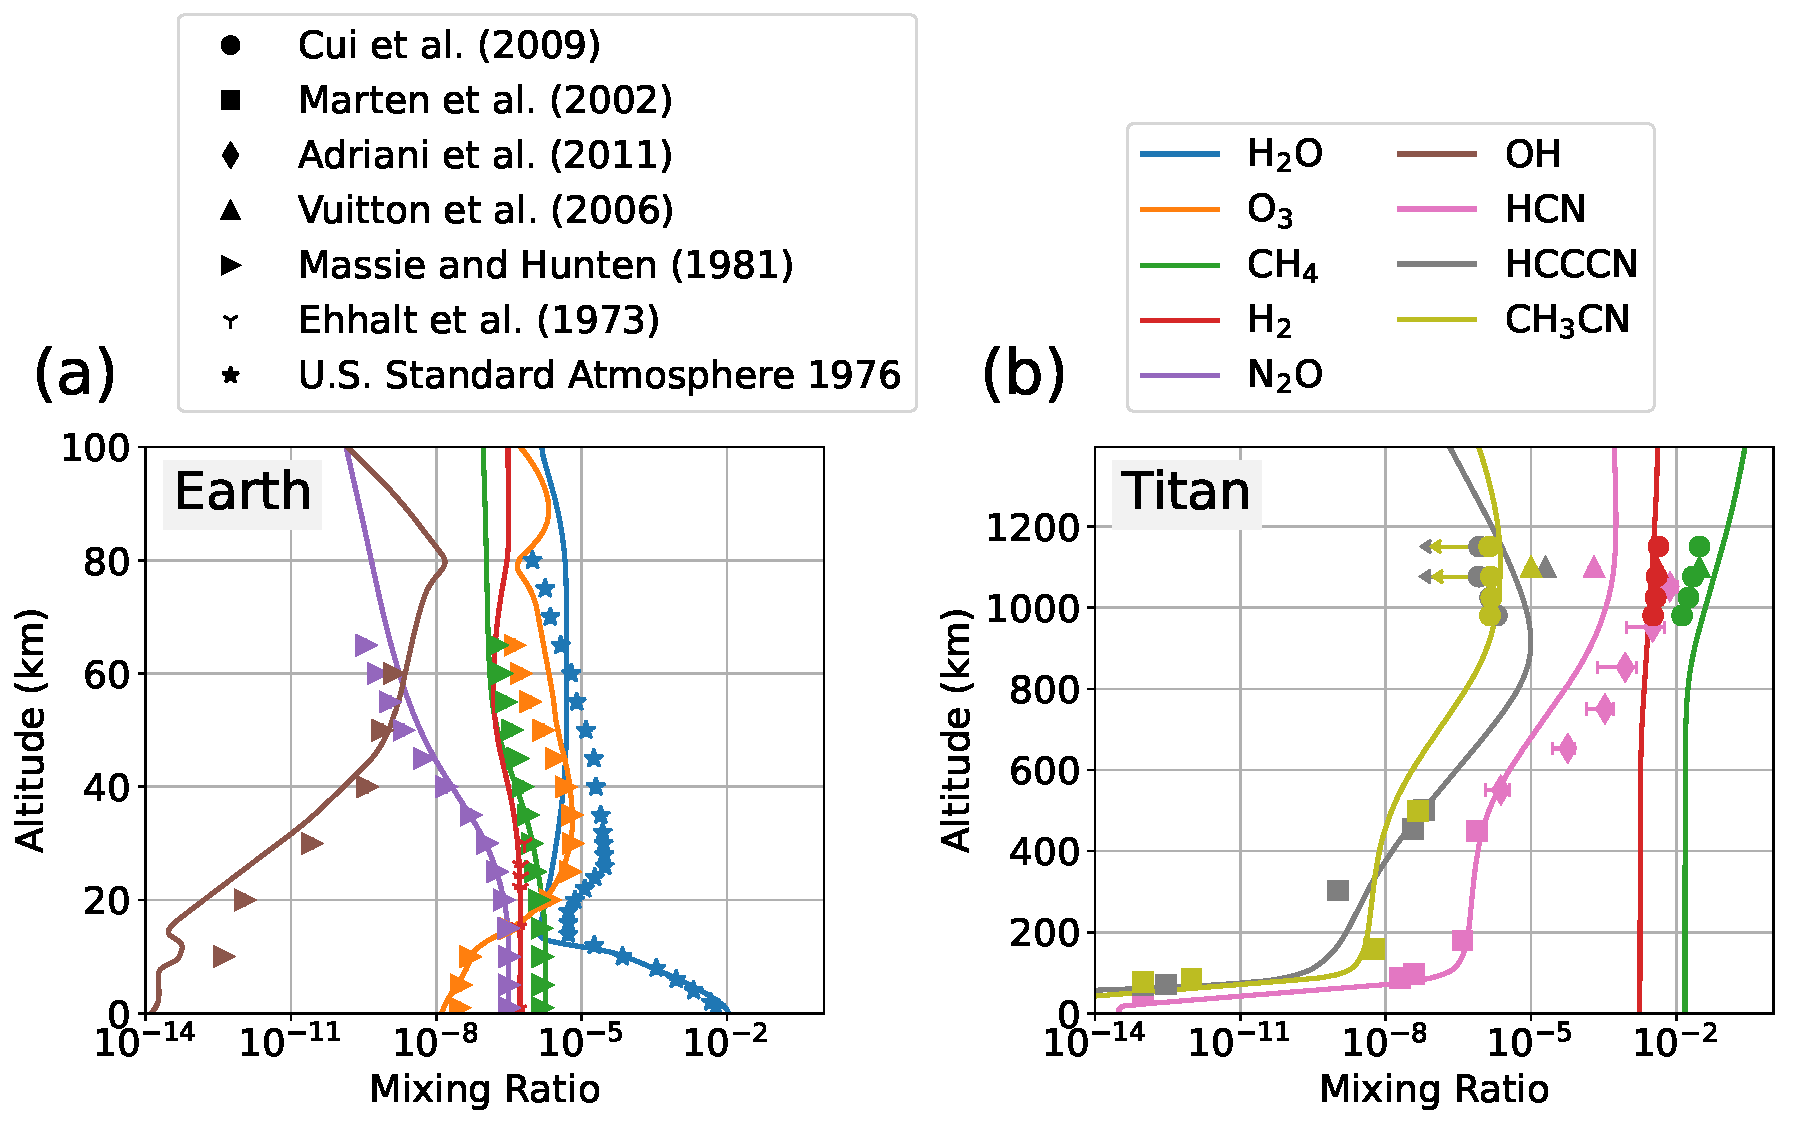
\includegraphics[width=0.9\textwidth]{tex/5impacts/figures/supplement/Earth_Titan_validation.pdf}
  \caption{Earth and Titan photochemical model validation. (a) and (b) shows the \emph{Photochem} model applied to Earth and Titan, respectively, compared to data from the literature \citep{Cui_2009,Marten_2002,Adriani_2011,Vuitton_2006,Massie_1981,Ehhalt_1975}.}
  \label{fig:earth_titan_valid}
\end{figure}

\subsubsection{Deposition velocity of HCN} \label{sec:hcn_vdep}

Our photochemical-climate simulations of post-impact atmosphere assume a HCN surface deposition velocity of $7 \times 10^{-3}$ cm s$^{-1}$. Here, we describe a simple model of HCN hydrolysis in the ocean which justifies this value.

Motivated by Appendix 3 in \citet{Kharecha_2005}, we imagine a two-box ocean model with a surface ocean of depth $\sim 100$ m and a deep ocean ($\sim 4$ km). We assume HCN transport into the ocean is governed by a stagnant boundary layer model (see Figure 3 in \citet{Kharecha_2005}), where it is destroyed by hydrolysis reactions. HCN is mixed between the surface and deep ocean reservoirs by a turnover velocity, $v_\text{over}$, which we nominally take to be $1.2 \times 10^{-5}$ cm s$^{-1}$ which is appropriate for modern Earth. Under these circumstances, the following system of ordinary differential equations governs the concentration of HCN in the surface and deep ocean.

\begin{gather}
  \frac{d m_\mathrm{HCN,s}}{dt} = \frac{\Phi_\mathrm{HCN}}{C z_s} - k_\mathrm{tot} m_\mathrm{HCN,s} - \left(\frac{v_\mathrm{over}}{z_s}\right)(m_\mathrm{HCN,s} - m_\mathrm{HCN,d}) \label{eq:hydro1}
  \\
  \frac{d m_\mathrm{HCN,d}}{dt} = - k_\mathrm{tot} m_\mathrm{HCN,s} + \left(\frac{v_\mathrm{over}}{z_d}\right)(m_\mathrm{HCN,s} - m_\mathrm{HCN,d}) \label{eq:hydro2}
\end{gather}

Here, $m_\mathrm{HCN,s}$ and $m_\mathrm{HCN,d}$ are the concentration of HCN in the surface and deep ocean, respectively, in mol L$^{-1}$, $C$ is a constant equal to $6.022 \times 10^{20}$ molecules mol$^{-1}$ L cm$^{-3}$, $z_s$ is the depth of the surface ocean, and $z_d$ is the depth of the deep ocean. We compute the temperature and pH dependent hydrolysis rate coefficient, $k_\mathrm{tot}$, following \citet{Miyakawa_2002}. $\Phi_\mathrm{HCN}$ is the HCN flux into the ocean in molecules cm$^{-2}$ s$^{-1}$, which is determined by a stagnant boundary layer model:

\begin{equation} \label{eq:flux_lid}
  \Phi_\mathrm{HCN} = v_\mathrm{p,HCN} (\alpha_\mathrm{HCN} 10^{-6} p_\mathrm{HCN} - m_\mathrm{HCN,s}) C
\end{equation}
We assume the piston velocity of HCN is $5 \times 10^{-3}$ cm s$^{-1}$, which is the same as the piston velocity of CO \citep[Table 1]{Kharecha_2005}. Also, $\alpha_\mathrm{HCN}$ is the henry's law coefficient for HCN. The flux of a gas can also be parameterized with a deposition velocity ($v_\mathrm{d,HCN}$):

\begin{align}
\begin{split}
  \Phi_\mathrm{HCN} &= n_\mathrm{HCN} v_\mathrm{d,HCN} \\
  &= \frac{p_\mathrm{HCN}}{k T} v_\mathrm{d,HCN} \label{eq:dep_vel}
\end{split}
\end{align}

Assuming a steady state ($d m_\mathrm{HCN,s}/dt = d m_\mathrm{HCN,d}/dt = 0$) and solving for $v_\mathrm{d,HCN}$ in Equations \eqref{eq:hydro1} - \eqref{eq:dep_vel} yields

\begin{equation}
  v_\mathrm{d,HCN} = 10^{-6} k T \alpha_\mathrm{HCN} C k_\mathrm{tot} v_\mathrm{p,HCN} \frac{k_\mathrm{tot} z_d z_s + v_\mathrm{over} (z_d + z_s)}{k_\mathrm{tot} z_d (v_\mathrm{p,HCN} + k_\mathrm{tot} z_s) + v_\mathrm{over}(v_\mathrm{p,HCN} + k_\mathrm{tot} (z_d + z_s))} \label{eq:HCN_vdep}
\end{equation}
Here, we assume that the temperature and pH of the ocean is uniform, and that the temperature of the surface air is the same as the temperature of the ocean. 

Figure \ref{fig:vdep_hcn} computes the deposition velocity of HCN using Equation \eqref{eq:HCN_vdep} over a wide range of ocean temperatures and pH. \citet{Kadoya_2020} used a model of the geologic carbon cycle to argue that the Hadean ocean was moderately alkaline (pH $\approx 8$). Therefore, we choose a HCN deposition velocity of $7 \times 10^{-3}$ cm s$^{-1}$ for our nominal model because it a reasonable approximation of the pH $= 8$ case over a wide range of temperatures. Additionally, we assume that HCCCN has the same deposition velocity as HCN, also caused by hydrolysis reactions in the ocean.

We have re-run our photochemical-climate simulations of post-impact atmospheres with order-of-magnitude larger and smaller HCN deposition velocities. The results are qualitatively unchanged. For example, assuming $v_\mathrm{d,HCN} = 7 \times 10^{-4}$ cm s$^{-1}$ for a $2 \times 10^{21}$ kg impactor in Figure \ref{fig:figure5} causes one order of magnitude smaller HCN ocean deposition. However, the HCN rainout and HCN surface pressure is unchanged because HCN rainout dominates over the HCN ocean deposition.

\begin{figure}
  \centering
  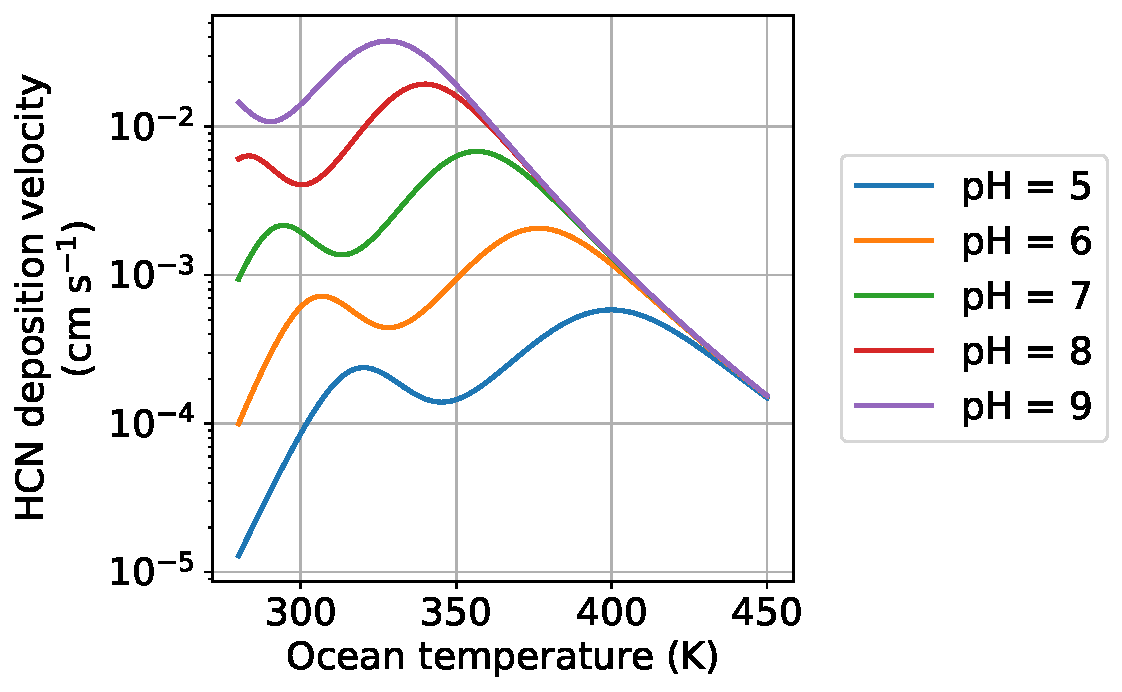
\includegraphics[width=0.6\textwidth]{tex/5impacts/figures/supplement/vdep_HCN.pdf}
  \caption{The deposition velocity of HCN caused by hydrolysis in the ocean. Calculations use Equation \eqref{eq:HCN_vdep} assuming $v_\mathrm{over} = 1.2 \times 10^{-5}$ cm s$^{-1}$, $z_s = 10^{4}$ cm, $z_d = 4 \times 10^{5}$ cm.}
  \label{fig:vdep_hcn}
\end{figure}

\subsection{The \emph{Clima} radiative transfer and climate model} \label{sec:clima}

To simulate the climate of post-impact atmospheres, we developed a new radiative transfer and climate code called \emph{Clima}. We approximately solve the radiative transfer equation using standard two-stream methods \citep{Toon_1989}. The code includes opacities representing photolysis, Rayleigh scattering, collision-induced absorption, and approximates line absorption with k-distributions. All available opacities and citations, except photolyisis cross sections, are listed in Table \ref{tab:climate_opacities}. In this article, to account for line absorption of multiple species, we use the ``random overlap with resorting and rebinning'' method described in \citet{Amundsen_2017}. 

Figure \ref{fig:early_mars_validation} shows a thermal emission spectra computed with \emph{Clima} for a two bar pure CO$_2$ atmosphere on Mars with a 250 K surface temperature. This same benchmark has been computed by several other radiative transfer codes: SOCRATES \citep[Figure 2]{Wolf_2022}, ExoRT \citep[Figure 2]{Wolf_2022}, SMART (Figure \ref{fig:early_mars_validation}), and the radiative transfer code used in \citet{Kopparapu_2013} (their Figure 1). All codes estimate the total outgoing thermal energy to be between 86 and 94 W m$^{-2}$, which is comparable to the value computed by \emph{Clima} (92.9 W m$^{-2}$).

The \emph{Clima} code also includes an adiabatic climate model. Given partial pressures of gases at the surface, the code draws a psuedoadiabat temperature profile upward using Equation (1) in \citet{Graham_2021} until the temperature reaches an assume isothermal stratosphere. The code is general and can consider any number of condensing species, but H$_2$O is the only relevant condensible for post-impact atmospheres. Finally, to find an equilibrium climate, we solve a nonlinear equation for the surface temperature that balances incoming solar and outgoing longwave radiation. Each iteration of the nonlinear solve involves drawing an adiabat upward then computing the solar and infrared radiative fluxes.

The version of \emph{Clima} used in this article (v0.3.1) is archived on Zenodo (\url{https://doi.org/10.5281/zenodo.7802952}), while the most up-to-date version can be found on GitHub (\url{https://github.com/Nicholaswogan/clima}).

\begin{spacing}{1.0}
\begin{center}
  \begin{tabularx}{\linewidth}{p{0.15\linewidth} | p{0.1\linewidth} | p{0.38\linewidth} | p{0.3\linewidth}} \caption{Opacities used in the \emph{Clima} radiative transfer code} \label{tab:climate_opacities} \\
    \hline \hline
    Opacity type & Opacity & Notes & Citation \\
    \hline 

    k-distributions$^\text{a}$ & H$_2$O & HITEMP2010 for 0 to 30,000 cm$^{-1}$ and HITRAN2016 for 30,000 to 42,000 $^{-1}$. Voigt line shape with 25 cm$^{-1}$ cutoff. Assumes Earth air broadening coefficients. Plinth or base is removed because this opacity is combined with MT\_CKD H$_2$O continuum. & \citet{Rothman_2010,Gordon_2017} \\

     & CO$_2$ & HITEMP2010. Sub-Lorentzian line shape with 500 cm$^{-1}$ cutoff. Assumes self-broadening coefficients. & \citet{Rothman_2010} \\

     & CH$_4$ & HITEMP2020. Voigt line shape with 25 cm$^{-1}$ cutoff. Assumes Earth air broadening coefficients. & \citet{Hargreaves_2020} \\

     & CO & HITEMP2019. Voigt line shape with 25 cm$^{-1}$ cutoff. Assumes self-broadening coefficients. & \citet{Li_2015} \\

     & O$_2$ & HITRAN2016. Voigt line shape with 25 cm$^{-1}$ cutoff. Assumes Earth air broadening coefficients. & \citet{Gordon_2017} \\

     & O$_3$ & HITRAN2016. Voigt line shape with 25 cm$^{-1}$ cutoff. Assumes Earth air broadening coefficients. & \citet{Gordon_2017} \\

    \hline

    CIA & H$_2$-H$_2$ & - & \citet{Molliere_2019} \\
    & H$_2$-He & - & \citet{Molliere_2019} \\
    & N$_2$-N$_2$ & - & \citet{Molliere_2019} \\
    & CH$_4$-CH$_4$ & - & \citet{Karman_2019} \\
    & N$_2$-O$_2$ & - & \citet{Karman_2019} \\
    & O$_2$-O$_2$ & - & \citet{Karman_2019} \\
    & H$_2$-CH$_4$ & - & \citet{Karman_2019} \\
    & CO$_2$-CO$_2$ & - & \citet{Karman_2019} \\
    & CO$_2$-CH$_4$ & - & \citet{Karman_2019} \\
    & CO$_2$-N$_2$ & - & \citet{Karman_2019} \\
    & N$_2$-H$_2$ & - & \citet{Karman_2019} \\

    \hline

    Rayleigh scattering$^\text{b}$ & N$_2$ & - & \citet{Keady_2002,Penndorf_1957} \\
    & CO$_2$ & - & \citet{Keady_2002,Shemansky_1972} \\
    & O$_2$ & - & \citet{Keady_2002,Penndorf_1957} \\
    & H$_2$O & - & \citet{Keady_2002,Ranjan_2017,Murphy_1977} \\
    & H$_2$ & - & \citet{Keady_2002} \\

    \hline

  \multicolumn{4}{p{1.0\linewidth}}{
    $^\text{a}$ All k-distributions are computed using HELIOS-K \citep{Grimm_2021}.

    $^\text{b}$ Rayleigh scattering opacities are computed using a parameterization from \citet{Vardavas_1984}.
  }

  \end{tabularx}
\end{center}
\end{spacing}

\begin{figure}
  \centering
  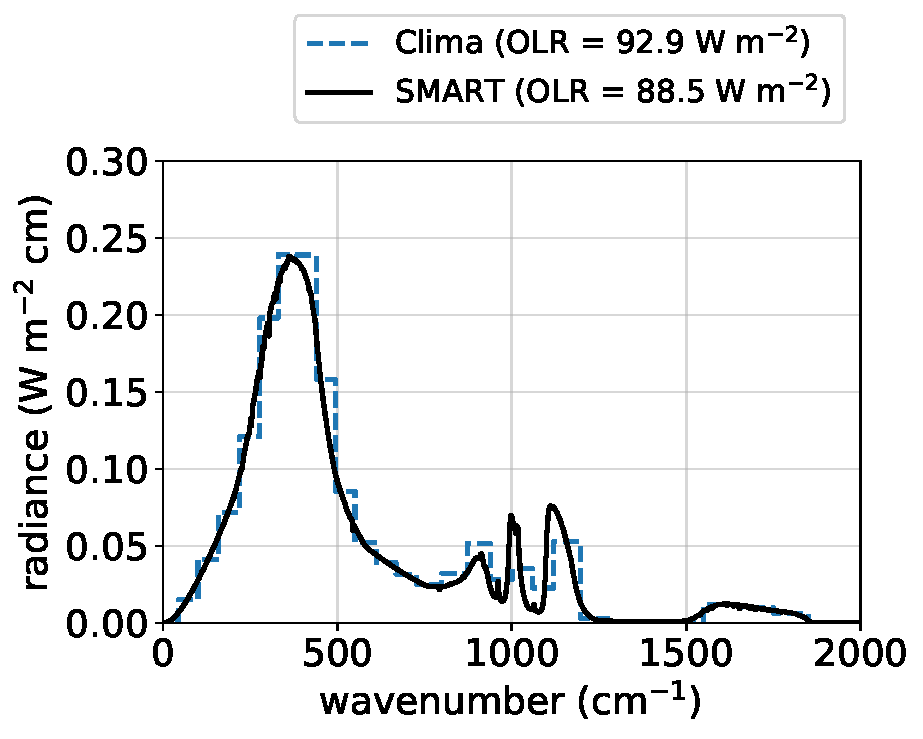
\includegraphics[width=0.5\textwidth]{tex/5impacts/figures/supplement/early_mars_validation.pdf}
  \caption{Outgoing longwave radiation of a 2 bar CO$_2$ atmosphere on Mars with a 250 K surface temperature, computed with \emph{Clima} (this work) and SMART \citep{Meadows_1996}. The agreement between the two codes validates \emph{Clima}.}
  \label{fig:early_mars_validation}
\end{figure}

\chapter{Timing and Likelihood of the Origin of Life Derived from Post-Impact Highly Reducing Atmospheres}
\newpage
\noindent \textit{This chapter was written in collaboration with David C. Catling and Kevin J. Zahnle, and will soon be submitted for publication in an academic journal.}

\section*{\centering Summary}

Big impacts on the early Earth would have created highly reducing atmospheres that generated molecules needed for the origin of life, such as nitriles. However, such impactors can be followed by collisions that were still sufficiently big to vaporize the ocean and destroy any pre-existing life. Thus, a post-impact reducing atmosphere that gives rise to life needs to be followed by a lack of subsequent sterilizing impacts for life to persist. Using statistics and limits for the impact history on early Earth and the impact mass needed to generate post-impact highly reducing atmospheres, we show that the median timing of impact-driven biopoiesis (i.e., the origin of life) is favored early in the Hadean eon. However, uncertainties are large because impact bombardment is stochastic, so biopoiesis could have occurred in $\sim 0.5$ billion year window from 4.45 to 3.9 Ga within 95\% uncertainty. Previous claims of a far narrower window for the origin of life are unsupported. In an optimistic scenario for life starting from post-impact reducing atmospheres, we find that the origin of life is possible in $\sim 90\%$ of stochastic impact realizations. In our most pessimistic case, life's origin is still fairly likely ($\sim 20\%$ chance). This potentially bodes well for life on rocky planets elsewhere because they will have experienced an early episode of enhanced impact bombardment given how planets form.

\section{Introduction}

\citet{Benner_2020} argued that the most likely time for the origin of life in an RNA-world scenario would have been $4.36 \pm 0.1$ Ga in the wake of a $\sim 2 \times 10^{22}$ kg ($\sim 2100$ km) asteroid impact called Moneta. They suggested that iron delivered by Moneta's core would have reacted with impact-vaporized ocean water to generate a reducing Hadean atmosphere conducive to the photochemical generation of essential prebiotic nitriles like HCN and HCCCN. Nitriles are required in prebiotic schemes that synthesize ribonucleotide precursors to RNA \citep{Patel_2015,Powner_2009,Becker_2019}. A transient period of profuse nitrile production after a Moneta impact could have been a window of opportunity for the origin of RNA and, ultimately, life.

A single Moneta impact could also explain the highly-siderophile elements (i.e. iron-loving, abbreviated HSEs) in the Moon's and the Earth's mantles. During the Moon-forming impact, HSEs should have been sequestered in each planetary core, so over-abundant HSEs in today's mantles are commonly interpreted as evidence for late-accretion impactors. Earth's mantle has substantially more HSEs than the Moon by an amount that cannot be accounted for by Earth's greater gravitational cross section \citep{Day_2015}. A single massive Moneta impact could explain the Earth-Moon HSE discrepancy because, by the statistics of small numbers, Moneta could have missed the Moon and hit the Earth \citep{Sleep_1989,Bottke_2010}.

However, the lunar HSE depletion may be explained without a Moneta impact. Lunar HSEs could have been lost to space during impact-delivery because of the Moon's small gravity \citep{Kraus_2015}. Alternatively, HSEs delivered to the Moon during its $\sim 150$ million-year magma ocean could have been sequestered in the core due to iron sulfide exsolution \citep{Morbidelli_2018,Rubie_2016}. Finally, there is some chance that the Earth's HSEs do not record late impacts because the Moon-forming impact delivered HSEs \citep{Sleep_2016}. Another explanation for Earth's HSEs that does not require impacts is that HSEs are gradual core contributions over time from mantle plumes \citep{Halliday_2023,Mundl_2020}. If indeed Earth's HSEs reflect asteroid bombardment after the Moon formed, then the HSEs can be explained by multiple $\sim 500$ to 2000 km impacts rather than a single big ($\sim 2100$ km) collision.

Chapter \ref{ch:5} and \citet{Zahnle_2020} used photochemical models of post-impact atmospheres to show that impacts significantly smaller than Moneta can efficiently produce prebiotic molecules. In their simulations, impactor iron equilibrates with vaporized ocean water to generate atmospheric H$_2$, CH$_4$ and NH$_3$ that form thermochemically as the reducing steam atmosphere cools. Once steam condenses to an ocean, subsequent photochemistry of a Titan-like, hazy atmosphere produces prebiotic nitriles. \citet{Zahnle_2020} was a preliminary study that used simple atmospheric models, and Chapter \ref{ch:5} improves upon their calculations with more sophisticated and accurate simulations. Photochemical modeling in Chapter \ref{ch:5} shows that the production of both HCN and HCCCN only occurs when $\mathrm{CH_4} / \mathrm{CO_2} \gtrsim 0.1$ while the atmosphere is hazy. In an optimistic scenario, which includes nickel-catalyzed methane production, results suggests that $\mathrm{CH_4} / \mathrm{CO_2} > 0.1$ (i.e. significant nitriles) occurs for impacts $> 4 \times 10^{20}$ kg ($> 570$ km diameter). In a pessimistic case, which assumes only a fraction of impactor iron reacts with the atmosphere \citep{Citron_2022}, a $> 5 \times 10^{21}$ kg ($> 1330$ km diameter) impactor is required to produce substantial HCN and HCCCN (Chapter \ref{ch:5}). Regardless of uncertainty, atmospheric models suggest that an impactor much smaller than Moneta could deliver the nitriles needed for an RNA origin of life.

Here, we use the Chapter \ref{ch:5} results, along with Monte-Carlo simulations of Earth's impact history, to make an alternative estimate for when life most likely emerged during an RNA-first process. Our calculations account for the possibility of planet sterilization by impacts that vaporize the ocean \citep{Sleep_1989}. We assume that a life-starting impact is one that produces significant prebiotic nitriles and is not subsequently followed by an ocean-vaporizing impact that destroys the biosphere. By considering the fraction of stochastic impact realizations that do not have a life-starting impact, we also estimate the probability of life beginning if Earth history was rerun.

\section{Methods} \label{sec:ch6_methods}

The rate impacts hit Earth bigger than mass $m$ at age $t$ can be written

\begin{equation}
  f(t,m) = F_0(t) S_0(m)
\end{equation}
Here, $S_0(m)$ is the size-frequency distribution of impactors normalized to a reference mass $m_0$ so that $S_0(m_0) = 1$. Also, $F_0(t)$ is the number of impacts per billion years with mass greater than $m_0$.

We assume that the the majority of the size-frequency distribution of impactors is identical to the main-belt asteroids \citep[Extended Data Figure 1 in][]{Marchi_2014}. Data for the frequency of main-belt asteroids only extends down to about 1 km diameter ($1.3 \times 10^{12} $ kg). To extend the distribution to smaller objects, we use the observed 1400 ratio between the frequency of $> 1$ km and $> 20$ km craters on the Moon following \citet{Morbidelli_2018}. Crater scaling relations suggest that 1 km and 20 km craters on the Moon corresponds to 50 m and 1 km asteroids, respectively \citep{Morbidelli_2018}. The largest main belt asteroid is $\sim 1000$ km, so we must extrapolate to larger impactors. Through the main text, we use the same extrapolation as \citet{Marchi_2014}, which extends the distribution to big impacts with a slope $d (\ln S_0)/d (\ln m) = - 0.415$ (Figure \ref{fig:sfd_and_flux}). In Chapter Appendix \ref{sec:append_sfd} we show that instead extrapolating with the red dashed line in Figure \ref{fig:sfd_and_flux}a (with slope $d (\ln S_0)/d (\ln m) = - 1.0$) does not significantly change our overall conclusions. Finally, we normalize the size-frequency distribution to the impact mass required to make a 1 km crater on the moon (50 m object, $m_0 = 1.64 \times 10^{8}$ kg). Figure \ref{fig:sfd_and_flux}a shows the resulting size-frequency distribution.

\begin{figure}
  \centering
  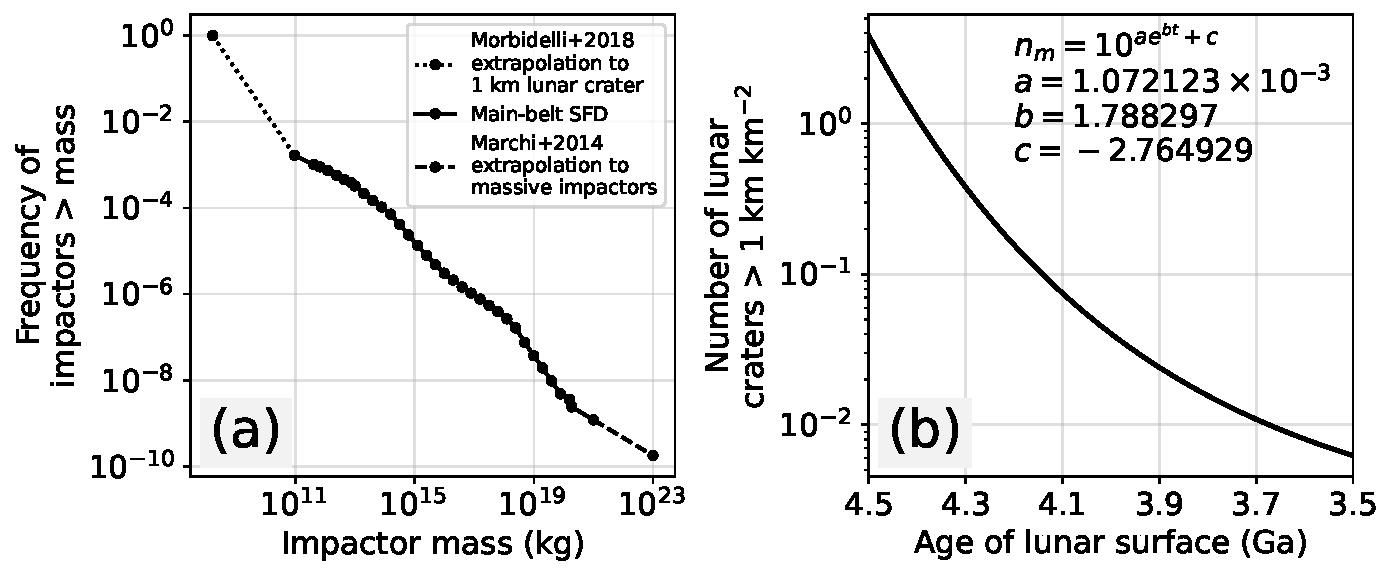
\includegraphics[width=1.0\textwidth]{tex/6time/figures/SFD_and_flux.pdf}
  \caption{Our assumed (a) size-frequency distribution of impactors and (b) lunar cratering record. Most of the size-frequency distribution is identical to the main-belt asteroids \citep[Extended Data Figure 1 in][]{Marchi_2014}. We extrapolate to objects $\lesssim 10^{11}$ kg using the observed frequency ratio of $> 1$ km and $> 20$ km lunar craters following \citet{Morbidelli_2018}, and, in the main text, log-log extrapolate to asteroids $\gtrsim 10^{21}$ kg following \citet{Marchi_2014}. In Chapter Appendix \ref{sec:append_sfd} we also consider the red dashed extrapolation to $\gtrsim 10^{21}$ kg impacts. The lunar cratering record is the red line in Figure 5 of \citet{Morbidelli_2018}.}`'
  \label{fig:sfd_and_flux}
\end{figure}

The flux of impactors, $F_0(t)$, can be estimated from the lunar cratering record. We adopt the accretionary tail scenario discussed in \citet{Morbidelli_2018}. In other words, we assume that the ``late heavy bombardment'' did not happen \citep{Cartwright_2022,Hartmann_2019,Zellner_2017}, and that the impact flux on Earth was monotonically decreasing throughout the Hadean eon. Figure \ref{fig:sfd_and_flux}b shows $n_m$, our assumed lunar impact history taken from \citet{Morbidelli_2018} (red line in their Figure 5). We use the parameterization $n_m = 10^{a e^{b t} + c}$, where $a$, $b$, and $c$ are fit parameters given in Figure \ref{fig:sfd_and_flux}b.

Extrapolating the lunar impact history to Earth requires correcting for Earth's greater gravitational attraction. Assuming that the approach velocity of impactors far from the Earth and Moon was on average 18 km/s \citep{Morbidelli_2018}, then Earth should receive $s_0 = 1.36$ times more impacts per surface area than the Moon. Therefore, the number of impacts on Earth is

\begin{equation}
  N_0 = A_\oplus s_0 n_m = A_\oplus s_0 10^{a e^{b t} + c}
  \label{eq:num_earth_impacts}
\end{equation}
Equation \eqref{eq:num_earth_impacts} also accounts for Earth's surface area ($A_\oplus$), making $N_0$ the number of impacts on Earth since age $t$ that would cause a crater $> 1$ km on the moon. As discussed previously, \citet{Morbidelli_2018} use crater scaling relations to show that a 1 km lunar crater corresponds to a 50 m object with mass $m_0 = 1.64 \times 10^8$ kg.

The time derivative of $N_0$ gives the flux, $F_0$:

\begin{equation}
  F_0(t) = \frac{d N_0}{dt}
\end{equation}
The average number of impacts on Earth between time $t_1$ and $t_2$ with mass greater than $m$ is then

\begin{align}
\begin{split}
  N(m,t_1,t_2) &= \int_{t_1}^{t_2} f(t,m) dt \\
  &= S_0(m) \int_{t_1}^{t_2} \frac{d N_0}{dt} dt \\
  &= S_0(m) A_\oplus s_0 \left( 10^{a e^{b t_2} + c} - 10^{a e^{b t_1} + c} \right)
\end{split}
\end{align}

To simulate impact histories, we consider a grid of $s\sim 200$ impactor masses between $10^{12}$ and $10^{23}$ kg, and a grid of $\sim 60$ times between 4.5 and 3.5 Ga. Indexes $j$ and $i$ indicate the mass and time grid cells respectively, while, for example, $j-\frac{1}{2}$ and $j+\frac{1}{2}$ indicate the edges of the grid cell. We can compute the expected number of impacts within a mass and time grid cell with the following

\begin{equation}
  \overline{N}_{ij} = N(m_{j-\frac{1}{2}},t_{i-\frac{1}{2}},t_{i+\frac{1}{2}}) - N(m_{j+\frac{1}{2}},t_{i-\frac{1}{2}},t_{i+\frac{1}{2}})
\end{equation}
Next, we sample a Poisson distribution for each $\overline{N}_{ij}$, giving a stochastic number of impacts in each mass and time grid cell which constitutes an impact history. By modeling impacts as a Poisson process, we are assuming that each impact does not change the probability of the next one (i.e., impacts are independent). Performing this sampling thousands of times captures many of the possible impact histories. We only keep impact histories that accrete a total mass of $2 \times 10^{22}$ to $6 \times 10^{22}$ kg because this is approximately the mass implied by the HSEs in Earth's mantle, assuming that HSEs were delivered by late accretion. This range of masses is based on \citet{Day_2015} who used mantle HSEs to suggest that the Earth was impacted by $\sim 3 \times 10^{22}$ to $4.8 \times 10^{22}$ kg of material, but we choose a wider range of masses because HSEs could have been lost to Earth's core or to space during impacts \citep{Marchi_2018}.

Our final step is to assign impact velocities to each collision in the many sampled impact histories. Figure \ref{fig:velocity_distribution} in the Chapter Appendix shows Earth's impact velocity distribution. We created this distribution using the JPL database of close approaches to Earth by small bodies \citep{Park_2023}, considering all close-approach asteroids within 0.05 AU to Earth. The database gives the approach velocity of each asteroid far from Earth, so we compute the impact velocity by accounting for Earth's gravitational potential energy. Here, we are assuming that the impact velocity distribution for small bodies (e.g. $< 10$ km) is identical to the velocity distribution for bigger asteroids (e.g. $> 10 km$). This may not be the case because small bodies are more strongly influenced by processes like the Yarkovsky effect \citep{Bottke_2006}, where an asteroid's orbit is altered by anisotropic thermal emission.

The final collection of sampled impact histories can then be used to compute impact statistics that are relevant to the timing and likelihood of the origin of life.

\section{Results} \label{sec:results}

\begin{figure}
  \centering
  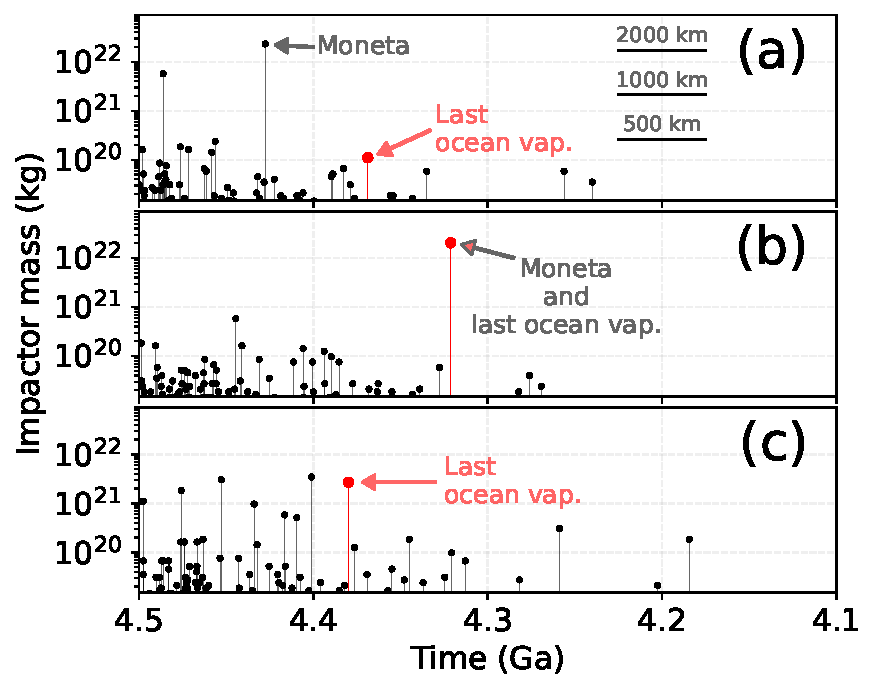
\includegraphics[width=0.7\textwidth]{tex/6time/figures/example_impact_histories.pdf}
  \caption{Three simulated impact histories of the 5000 derived from our Monte-Carlo approach (Section \ref{sec:ch6_methods}). Each vertical line indicates an impact of a mass shown by the y-axis. The red lines indicate the last impact to vaporize the ocean assuming 10\% of an impacts kinetic energy heats the ocean. (a) gives conversions between impact mass and diameter for 500, 1000 and 2000 km asteroids.}
  \label{fig:example_impact_histories}
\end{figure}

Figure \ref{fig:example_impact_histories} illustrates three of the 5000 impact histories computed with our Monte-Carlo approach (Section \ref{sec:ch6_methods}). In Figure \ref{fig:example_impact_histories}a, a Moneta-sized impact occurs at $\sim 4.43$ Ga delivering nearly all of Earth's mantle HSEs. The impact should also reduce the Hadean atmosphere creating conditions favorable for prebiotic chemistry. However, in this case, Moneta is not a life-starting impact because Moneta is followed by an ocean-vaporizing collision at $\sim 4.37$ Ga which we assume destroys any existing biosphere. Based on smoothed-particle hydrodynamics impact simulations, we nominally assume that 10\% of an impact's kinetic energy goes into vaporizing the ocean \citep[Chapter Appendix \ref{sec:append_vap},][]{Citron_2022}. Vaporizing the ocean requires $5 \times 10^{27}$ J, so a $> 5 \times 10^{28}$ J impact should deliver sufficient energy under our assumptions. Chapter Appendix \ref{sec:append_vap} considers alternative criteria for ocean-vaporization. In Figure \ref{fig:example_impact_histories}a, the last ocean-vaporizing impact is only $\sim 10^{20}$ kg (360 km) but has a large impact velocity of $32$ km/s giving it $5.12 \times 10^{28}$ J of kinetic energy. 

Moneta also occurs in the Figure \ref{fig:example_impact_histories}b impact realization. In this scenario, any life created in the wake of Moneta will not be subsequently impact-exterminated because Moneta is the last impact to vaporize the ocean.

Figure \ref{fig:example_impact_histories}c shows an impact history where Moneta does not occur. Instead, Earth's mantle HSEs are delivered by multiple $10^{21}$ to $4 \times 10^{21}$ kg collisions. Whether this bombardment history would cause biopoiesis depends on the required minimum impact mass to produce significant origin-of-life nitriles (e.g. HCN and HCCCN). Chapter \ref{ch:5} uses photochemical models of post-impact atmospheres to show that, optimistically, an impact $> 4 \times 10^{20}$ kg should give rise to an atmosphere that makes significant HCN and HCCCN. Under this optimistic requirement, the last ocean-vaporizing impact in Figure \ref{fig:example_impact_histories}c could successfully start life and occurs at 4.38 Ga with mass $3 \times 10^{21}$ kg. However, with pessimistic modeling assumptions, Chapter \ref{ch:5} finds that a $> 5 \times 10^{21}$ kg impactor is instead required for substantial nitrile delivery to the surface. In this alternative scenario, an origin of life never occurs in Figure \ref{fig:example_impact_histories}c because there is no impactor larger than $5 \times 10^{21}$ kg.

\begin{figure}
  \centering
  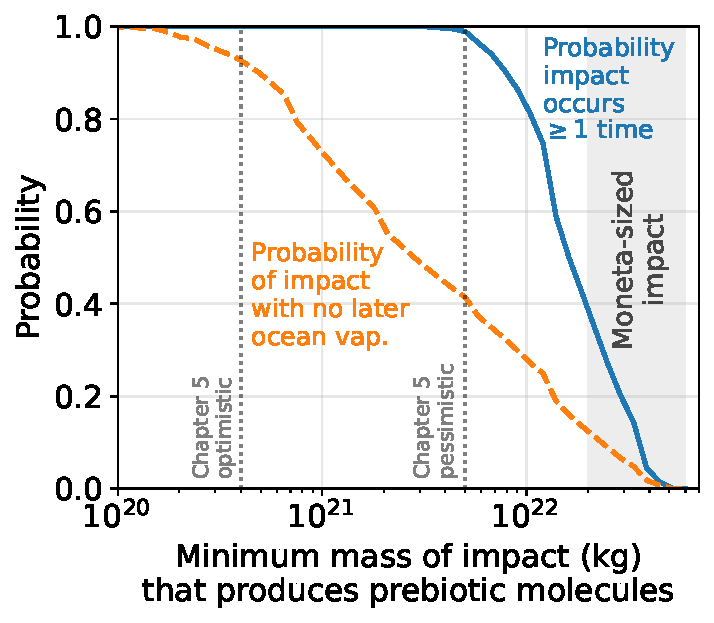
\includegraphics[width=0.55\textwidth]{tex/6time/figures_thesis/probabilities_of_impacts.pdf}
  \caption{The probability of an impact that causes favorable conditions for an origin of life on Earth. The blue solid line is the probability of an impact occurring at least once. The orange dashed line is the probability of an impact without a subsequent ocean-vaporizing collision. Probabilities are shown as a function of the minimum impact mass to produce significant prebiotic molecules (e.g. HCN). Two plausible minimum masses are the Chapter \ref{ch:5} optimistic and pessimistic scenarios indicated with vertical dotted lines. The shaded region between $2 \times 10^{22}$ and $6 \times 10^{22}$ kg are Moneta-sized impacts because they deliver most all of Earth's mantle HSEs. There is a 92\% chance of an impact creating favorable origin of life conditions in the Chapter \ref{ch:5} optimistic case, and a 41\% chance in the pessimistic case.}
  \label{fig:probabilities_of_impacts}
\end{figure}

As illustrated in Figure \ref{fig:example_impact_histories}, a life-starting impact does not occur in every simulated impact history. In our impact-driven model for the origin of life, biopoiesis requires (1) an impact of sufficient mass to make prebiotic nitriles and (2) the lack of a later ocean-vaporizing collision that destroys the biosphere without rekindling it. Figure \ref{fig:probabilities_of_impacts} shows the probability of both conditions occurring as a function of the minimum impact mass that produces prebiotic molecules. For example, consider the Chapter \ref{ch:5} optimistic minimum mass of $4 \times 10^{20}$ kg indicated in Figure \ref{fig:probabilities_of_impacts}. All simulated impact histories have at least one impact bigger than $4 \times 10^{20}$ kg (blue line in Figure \ref{fig:probabilities_of_impacts} is 1.0 at the given mass). However, the probability of the origin of life in this scenario is 92\%, because 8\% of the time the last $4 \times 10^{20}$ kg collision is followed by a smaller ocean-vaporizing impact that perhaps sterilizes the planet (orange dashed line in Figure \ref{fig:probabilities_of_impacts} with 0.92 at $4 \times 10^{20}$ kg). An origin of life is less probable if we consider the Chapter \ref{ch:5} pessimistic minimum mass ($> 5 \times 10^{21}$ kg) to produce significant origin-of-life nitriles. A $> 5 \times 10^{21}$ kg impact without later ocean vaporization occurs 41\% of the time. A life-starting impact was therefore relatively likely on the early Earth, and was strongly favored (92\% probability) under optimistic assumptions.

\begin{figure}
  \centering
  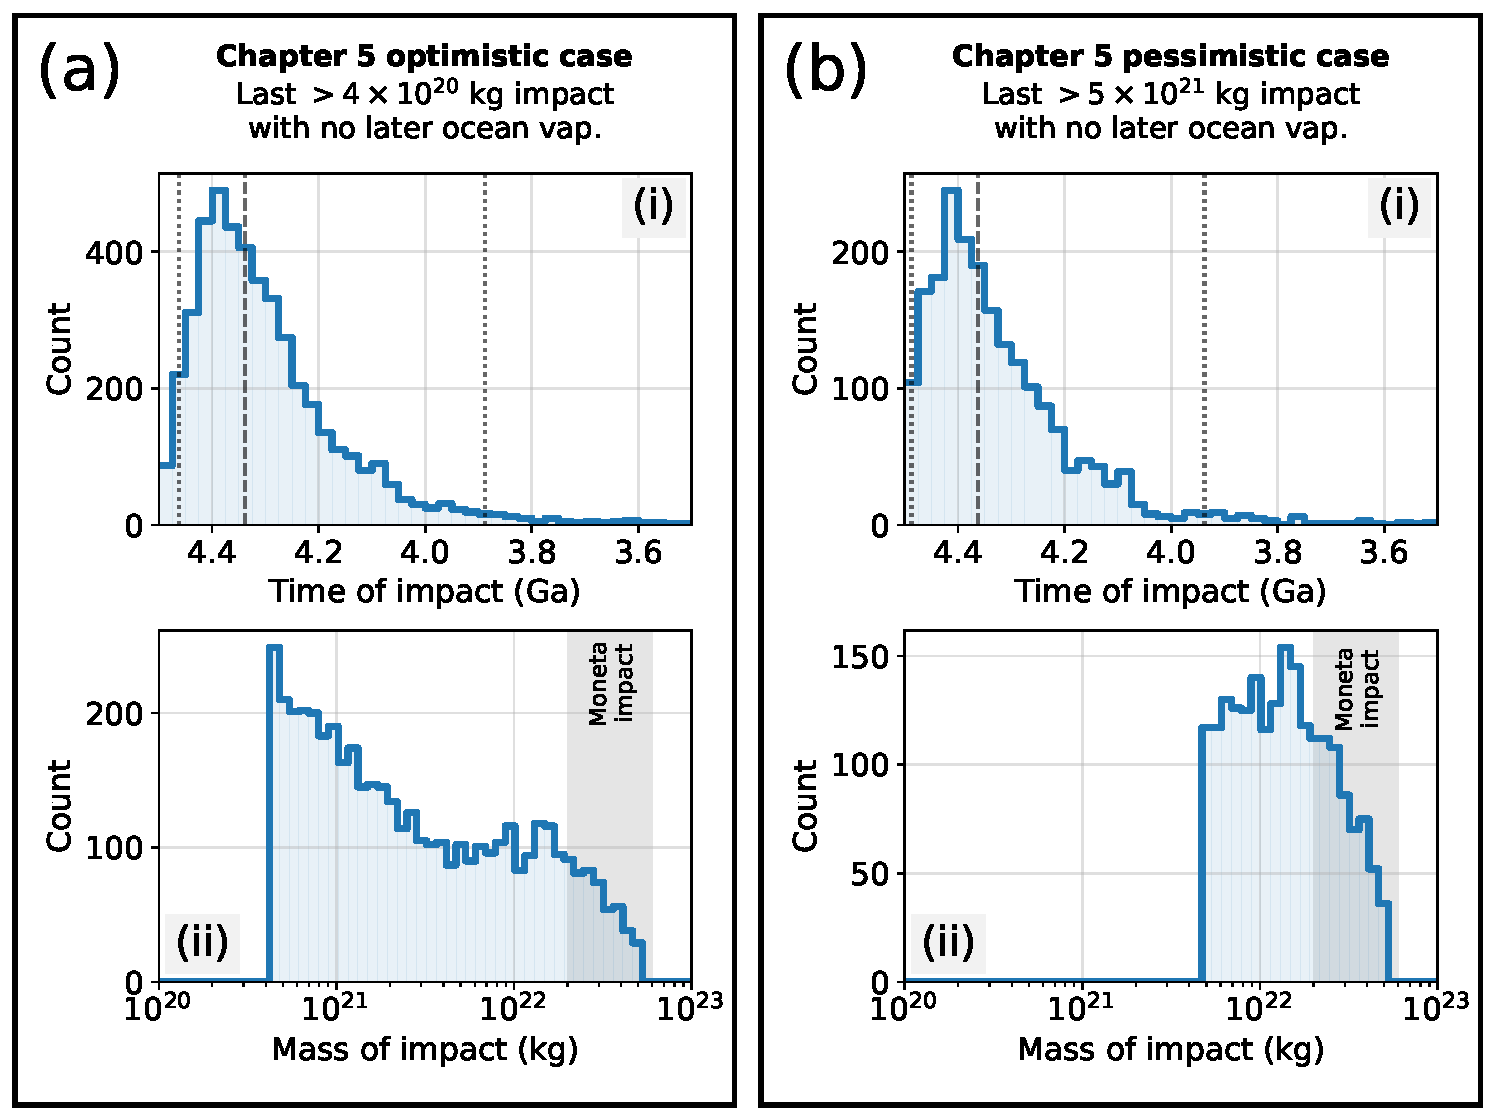
\includegraphics[width=1.0\textwidth]{tex/6time/figures_thesis/timing_and_mass.pdf}
  \caption{The timing and mass of a life-starting impact on the early Earth. (a) considers an optimistic minimum impact mass needed to generate the molecules for an RNA origin of life and (b) examines a pessimistic minimum impact mass Chapter \ref{ch:5}. In either (a) or (b), panels (i) and (ii) show probability distributions for the timing and mass, respectively, of the last impact the produces prebiotic molecules which does not have a later ocean-vaporizing collision. The vertical dashed lines on (a) i and (b) i plot are median values, and the vertical dotted lines are the 95\% confidence intervals. In an impact-driven origin of life, biopoiesis most likely occurred at $4.34$ Ga (95\% CI: 3.89 to 4.46 Ga) assuming panel (a) and at $4.36$ Ga (95\% CI: 3.94 to 4.49 Ga) assuming panel (b).}
  \label{fig:time_and_mass}
\end{figure}

To estimate the most likely timing for the origin of life, we consider both the optimistic and pessimistic criteria of Chapter \ref{ch:5}. Figure \ref{fig:time_and_mass}a is the optimistic case, showing the timing (Figure \ref{fig:time_and_mass}a (i)) and mass (Figure \ref{fig:time_and_mass}a (ii)) of the last $> 4 \times 10^{20}$ kg impactor for the 92\% of impact histories that do not experience later ocean vaporization. The median timing of a life-starting impact is 4.34 Ga with 95\% uncertainty between 3.89 and 4.46 Ga. The large uncertainty mostly stems from the stochastic, Poisson nature of asteroid bombardment. The probability distribution for the mass of the life-starting impact peaks at $4 \times 10^{20}$ kg and decreases with increasing mass because of the size-frequency distribution of asteroids (Figure \ref{fig:sfd_and_flux}a). There is only a 10\% chance that the impactor is Moneta-sized (i.e., between $2 \times 10^{22}$ and $6 \times 10^{22}$ kg).

The timing of an origin of life impact is qualitatively unchanged when instead adopting the Chapter \ref{ch:5} pessimistic case, which requires a $> 5 \times 10^{21}$ kg impact without later ocean vaporization (Figure \ref{fig:time_and_mass}b). In this scenario, the median timing for life's origin is 4.36 Ga with a 95\% confidence interval spanning 3.94 to 4.49 Ga (Figure \ref{fig:time_and_mass}b (i)). Under these assumptions, the life-starting impact is Moneta-sized 31\% of the time (Figure \ref{fig:time_and_mass}b (ii)), which is more probable compared to ``optimistic'' case (Figure \ref{fig:time_and_mass}a (ii)).

In this model for biopoiesis, life would probably start approximately within 10s of millions of years after a life-starting impact because this is the maximum duration of the H$_2$- and CH$_4$- rich atmosphere that makes nitriles like HCN (Chapter \ref{ch:5}). We ignore the $< 10$s million year span between an impact and life's origin because it is small compared to our $\sim 500$ million-year uncertainty for the timing of a life-starting impact.

\section{Discussion}

Our estimated timing for biopoiesis is compatible with the earliest well-accepted geologic evidence of life in the form of stromatolites in the 3.5 Ga Pilbara block of western Australia \citep{Walter_1980,Buick_1981,Van_2018}. Older geologic evidence of life exists, such as a $> 3.7$ Ga black shale metamorphosed to graphite with negative $\delta^{13}$C characteristic of biology \citep{Rosing_1999,Ohtomo_2014}. Also, \citet{Bell_2015} discovered graphite inclusions in a 4.1 Ga zircon grain with $^{13}$C depletions compatible with biological activity, but this is a tentative biosignature because there are abiotic mechanisms for making isotopically light carbon \citep{Javaux_2019}. If the \citet{Bell_2015} finding is indeed a sign of life, then it would be generally compatible with our estimated timing in Figure \ref{fig:time_and_mass}, because we find that there is only a $\sim 10\%$ chance of life starting after 4.1 Ga.

Furthermore, Hadean zircons provide some constraint on Earth's impact history which we do not explicitly account for in our calculations. The oldest zircons are from Jack Hills, Australia, with U-Pb dates as old as $\sim 4.38$ Ga \citep{Valley_2014}. \citet{Benner_2020} argued that a Moneta-scale impact ($\sim 2 \times 10^{22}$ kg) could not have occurred after this date, because such a collision would heat the crust enough to potentially reset all U-Pb chronometers. \citet{Benner_2020} makes this claim based on \citet{Abramov_2013}, who used models of impact ejecta coupled to simulations of radiogenic Pb-loss in zircons to investigate chronometers resetting during the hypothesized ``late-heavy bombardment''. However, \citet{Abramov_2013} considers impacts much smaller than Moneta (e.g. $< 10^{21}$ kg), and does not clearly establish a minimum impactor mass that would reset all zircon chronometers globally. Given this ambiguity, our simulations do not use zircon chronometers as a constraint on Earth's impact history.

Even if an impact failed to reset a zircon chronometer, the shock wave produced by an asteroid collision may create micro- to nano-structural features in zircons that could be preserved over billions of years \citep{Reimink_2023}. Therefore, the presence or absence of shocked Hadean zircons in the geologic record may provide some constraint on Earth's impact history. For example, \citet{Reimink_2023} estimated the probability of preserved zircons with shock features assuming Earth experienced a ``late-heavy bombardment'' at 3.9 Ga. In this scenario, they find that shocked zircons were likely preserved yet find none in a collection of 4.02 Ga zircons from the Acasta Gneiss Complex. Overall, the absence of preserved shocked zircons suggests that a ``late-heavy bombardment'' did not occur at 3.9 Ga. Our Monte-Carlo models of Earth's impact history do not use zircon shock features as a constraint. A better model would incorporate this information.

It is temping to extrapolate our results beyond the early Earth to exoplanets, but we must do so with caution because planets orbiting different stars may have bombardment histories unlike the Hadean. Planets in the habitable zone of a late M-type star during the stellar main-sequence phase were interior to the habitable zone for several hundred million years during the super luminous pre-main-sequence phase \citep{Luger_2015}. \citet{Lichtenberg_2022} use N-body simulations to show that, for planets hosted by late M-dwarfs, large asteroid impacts are not useful for prebiotic chemistry because big impacts most likely occur within 100 million years of planet formation during the stellar pre-main-sequence when the planet is outside of the habitable zone. The pre-main-sequence phase is not an issue for an impact-induced origin of life on planets orbiting sun-like stars because the phase only lasts $\sim 3$ Myrs, while large asteroid impacts occur for 100s Myrs \citep{Lichtenberg_2022}. Therefore, our result that a life-starting impact was likely on the early Earth (92\% chance in an optimistic case) might be best extrapolated to habitable zone exoplanets orbiting sun-like stars.

A caveat to our results is that ocean-vaporization by an impact is likely a complicated function of impact mass, velocity, and incident angle, which we do not account for (Chapter Appendix \ref{sec:append_vap}). Throughout Section \ref{sec:results} we have assumed that 10\% of an impactor's kinetic energy heats the planetary surface ($f_\mathrm{E,vap} = 0.1$), leading to a required $> 5 \times 10^{28}$ J collision to vaporize an ocean. Figure \ref{fig:energy_for_ocean_vap} in the Chapter Appendix uses simulations of impacts from \citet{Citron_2022} to show that $f_\mathrm{E,vap} = 0.1$ is a reasonable assumption, but that values between 2.5\% and 25\% are also possible and that $f_\mathrm{E,vap}$ likely also depends on impact angle.

To determine the sensitivity of our results to $f_\mathrm{E,vap}$, we recomputed the likelihood and timing of an impact that starts life in Chapter Appendix \ref{sec:append_vap} using $f_\mathrm{E,vap} = 0.025$ and $f_\mathrm{E,vap} = 0.25$. We find that the probability of a life-starting impact is somewhat sensitive to $f_\mathrm{E,vap}$, while the timing does not depend strongly on $f_\mathrm{E,vap}$. Overall, this uncertainty does not change our qualitative conclusion that an origin of life impact on the early Earth was not a fluke. Even in our worst-case scenario (i.e., Chapter \ref{ch:5} pessimistic case with $f_\mathrm{E,vap} = 0.25$) a life-starting impact occurs in 20\% of impact realizations (Figure \ref{fig:probabilities_of_impacts_sens} in the Chapter Appendix). Additionally, uncertainty in $f_\mathrm{E,vap}$ does not change our general conclusion that the most likely timing for the origin of life was $\sim 4.35$ Ga, with 95\% uncertainty spanning the Hadean eon (Figure \ref{fig:timing_sensitivity} in the Chapter Appendix). However, a more complete understanding of $f_\mathrm{E,vap}$ as a function of impact angle and other similar parameters may change this result.

An additional related caveat is that our calculations assume that an impact that vaporizes the ocean also sterilizes the planet, but this may not be the case because microbes might have survived in the deep subsurface \citep{Sleep_1989,Grimm_2018}. If ocean-vaporization does not destroy the biosphere, then our results would favor an origin of life earlier than we predict in Figure \ref{fig:time_and_mass}, and a life-starting impact would also be more probable than we have estimated (Figure \ref{fig:probabilities_of_impacts}).

\section{Conclusions}

We use Monte-Carlo simulations of Earth's impact history to determine the most likely timing for the origin of life that requires early ribonucleobase synthesis. We use the results of Chapter \ref{ch:5}, which finds that significant origin of life precursor molecules, such as HCN, are produced in the Hadean atmosphere after a $> 4 \times 10^{20}$ kg impact in an optimistic case, and after a $> 5 \times 10^{21}$ kg impact in a pessimistic scenario. We consider both possibilities, and assume such impacts can cause life's origin so long as they are not followed by a smaller ocean-vaporizing collision that sterilizes the planet.

For either the optimistic or pessimistic cases, we find that the most likely timing for an origin of life impactor is $\sim 4.35$ Ga with a 95\% uncertainty spanning the entire Hadean eon (approximately 4.45 to 3.9 Ga). The large uncertainty is caused by the intrinsic stochastic nature of impacts. These results suggest that the \citet{Benner_2020} proposed timing of the origin of life, at $4.36 \pm 0.1$ Ga, is too narrow. Furthermore, the mass of the life-starting impactor is most likely (69\% to 90\% probability) smaller than the Moneta impactor (Figure \ref{fig:time_and_mass}) proposed by \citet{Benner_2020}, because the size frequency distribution of asteroids prefers more frequent smaller impactors.

Our simulations of Earth's impact history do not always result in a bombardment favorable for an origin of life. There are some impact histories where a collision of sufficient mass to produce prebiotic molecules does not occur, or alternatively, does occur but primitive life is subsequently destroyed by an ocean-vaporizing impact that does not rekindle the biosphere. With our nominal assumptions, a life-starting impact occurs 92\% or 41\% of the time when we assume a $> 4 \times 10^{20}$ kg or $> 5 \times 10^{21}$ kg impact without later ocean-vaporization is required to start life, respectively. In our worst-case scenario, which assumes that impacts can more easily vaporize the ocean, a $> 5 \times 10^{21}$ kg impact without subsequent planet sterilization occurs in 20\% of simulated impact histories (Figure \ref{fig:probabilities_of_impacts_sens} in the Chapter Appendix).

If life began after an impact that generated a reducing atmosphere, then this work suggests that origin of life on Earth was fairly likely (at least a 20\% chance) and was indeed strongly favored (92\% chance) under optimistic assumptions. Given that rocky planets form from accretionary impacts, our work supports an optimistic outlook for life on exoplanets orbiting sun-like stars and future searches for biosignatures.

\section{Chapter Appendix}

\subsection{Size-frequency distribution sensitivity test} \label{sec:append_sfd}

\begin{figure}
  \centering
  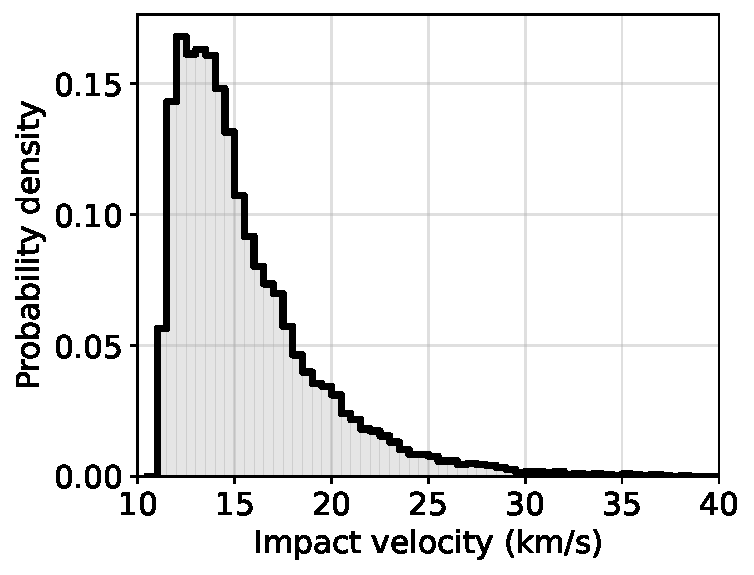
\includegraphics[width=0.5\textwidth]{tex/6time/figures/velocity_distribution.pdf}
  \caption{Our assumed probability distribution for the velocity of impacts derived from modern observations of asteroid close approaches \citep{Park_2023}.}
  \label{fig:velocity_distribution}
\end{figure}

We assume that the size-frequency distribution of objects that struck the early Earth is similar to the main-belt asteroids. A problem with this approach is that the main-belt asteroids only contain objects up to $\sim$ 1000 km diameter, yet the early Earth is expected to have experience impacts larger than this \citep{Marchi_2014}. Therefore, we must extrapolate the size-frequency distribution above $\sim$ 1000 km to larger objects. Throughout the main text we use the same extrapolation as \citet{Marchi_2014} (the black dashed line in Figure \ref{fig:sfd_and_flux}), who extends the size-frequency distribution with a log-log slope of $d (\ln S_0)/d (\ln m) = - 0.415$.

To test the sensitivity of our results to this chosen extrapolation, we re-did our Monte-Carlo analysis using a log-log slope of $d (\ln S_0)/d (\ln m) = - 1$ (the red dashed line in Figure \ref{fig:sfd_and_flux}) for impactors bigger than $\sim$ 1000 km diameter. Figures \ref{fig:probabilities_of_impacts_extrapolation_sens} and \ref{fig:timing_extrapolation_sensitivity} show how our results change when adopting this alternative extrapolation. Overall, our results are qualitatively unchanged for the different extrapolation slope ($d (\ln S_0)/d (\ln m)$).

\begin{figure}
  \centering
  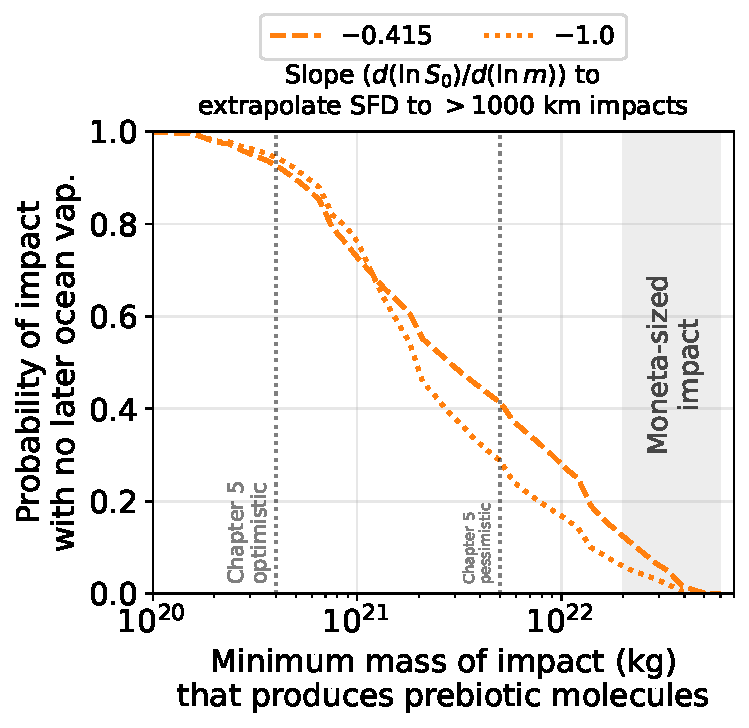
\includegraphics[width=0.55\textwidth]{tex/6time/figures_thesis/probabilities_of_impacts_extrapolation_sens.pdf}
  \caption{Similar to Figure \ref{fig:probabilities_of_impacts}, except we consider different extrapolations of the size-frequency distribution (SFD) for impactors larger than 1000 km diameter. The line labeled $d (\ln S_0)/d (\ln m) = - 0.415$ is the black dashed extrapolation in Figure \ref{fig:sfd_and_flux}a. The $d (\ln S_0)/d (\ln m) = - 1.0$ case is shown by the red dashed extrapolation in Figure \ref{fig:sfd_and_flux}a.}
  \label{fig:probabilities_of_impacts_extrapolation_sens}
\end{figure}

\begin{figure}
  \centering
  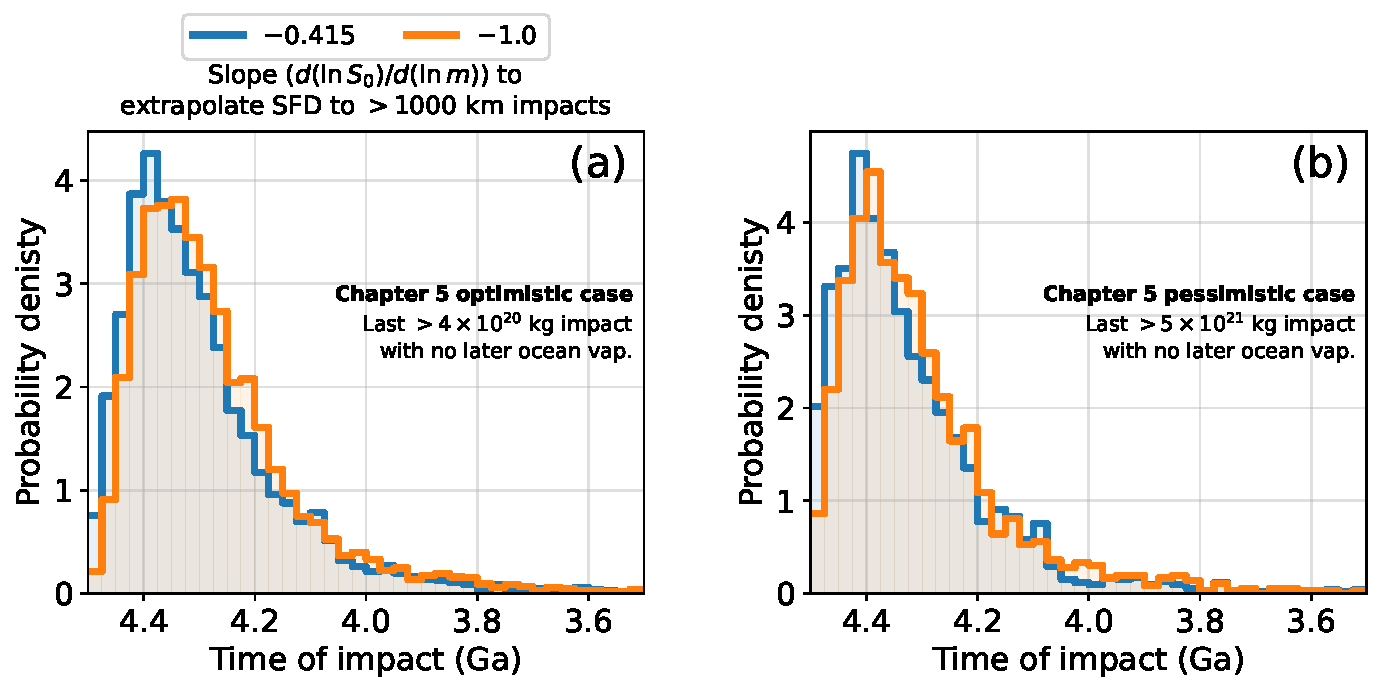
\includegraphics[width=1.0\textwidth]{tex/6time/figures_thesis/timing_extrapolation_sensitivity.pdf}
  \caption{Similar to Figure \ref{fig:time_and_mass}, except we consider different extrapolations of the size-frequency distribution (SFD) for impactors larger than 1000 km diameter. The line labeled $d (\ln S_0)/d (\ln m) = - 0.415$ is the black dashed extrapolation in Figure \ref{fig:sfd_and_flux}a. The $d (\ln S_0)/d (\ln m) = - 1.0$ case is shown by the red dashed extrapolation in Figure \ref{fig:sfd_and_flux}a.}
  \label{fig:timing_extrapolation_sensitivity}
\end{figure}

\subsection{Impact energy required for ocean vaporization} \label{sec:append_vap}

Recently, \citet{Citron_2022} performed smoothed-particle hydrodynamics impact simulations over a range of impact angles, masses and velocities to estimate the impact properties that can vaporize an ocean. Figure \ref{fig:energy_for_ocean_vap}a shows their simulation results for the change in the atmosphere's and ocean's internal energy ($\Delta \mathrm{IE}_\mathrm{atmo}$) as a function of impact kinetic energy ($\mathrm{E}_\mathrm{imp}$), along with log-log extrapolations for each impact angle. Figure \ref{fig:energy_for_ocean_vap} gives the same information, but the y-axis is instead the fraction of the impactor's energy that heats the atmosphere and ocean over the course of their simulations. For the most probable incident impact angle of $45^\circ$ about $\sim 10\%$ of the impactors kinetic energy heats the atmosphere ($f_\mathrm{E,vap} = 0.1$), so we nominally adopt this value in the main text to determine which collisions vaporize the ocean.

Energy delivery to the atmosphere/ocean appears to depend on impact angle, mass and velocity (Figure \ref{fig:energy_for_ocean_vap}). Additionally, all of the \citet{Citron_2022} simulations are far more massive than the minimum threshold for ocean-vaporization, so we must rely on extrapolations. Therefore, our assumption of a constant $f_\mathrm{E,vap} = 0.1$ is an over-simplification. To remedy this shortcoming, we considered building a parameterization for $f_\mathrm{E,vap}$ that depends on multiple impact properties (e.g., impact angle) using the \citet{Citron_2022} simulation results, but this was unsuccessful because their calculations do not consider a wide enough parameter space.

\begin{figure}
  \centering
  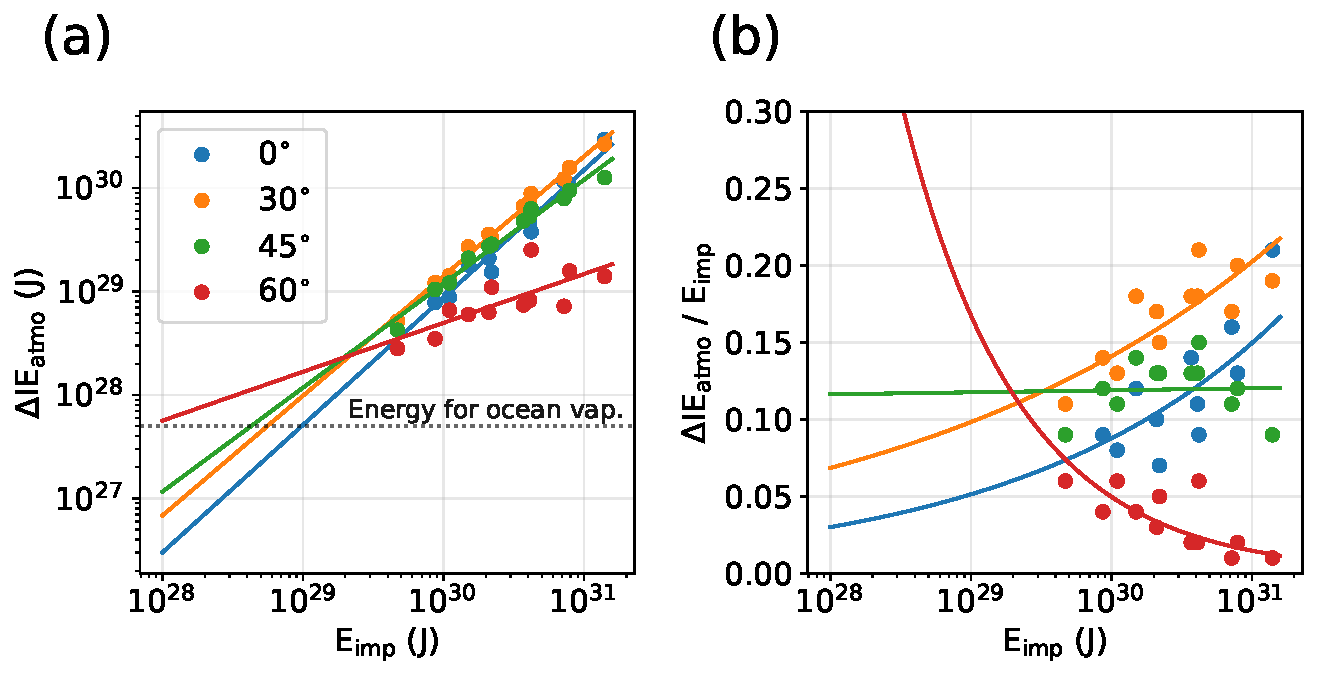
\includegraphics[width=1.0\textwidth]{tex/6time/figures/energy_for_ocean_vap.pdf}
  \caption{\citet{Citron_2022} smoothed-particle hydrodynamics simulations that show how much impactor kinetic energy heats the atmosphere and ocean. Different colors indicated various incident impact angles. (a) shows the simulated change in internal energy of the atmosphere and ocean as a function of the impactor energy, with linear log-log extrapolations for each impact angle. The dotted horizontal line at $5 \times 10^{27}$ J indicates the energy needed to vaporize an ocean \citep{Sleep_1989}. (b) contains the same information as (a), except the y-axis is the fraction of impactor energy that heats the atmosphere and ocean.}
  \label{fig:energy_for_ocean_vap}
\end{figure}

The evaluate the sensitivity of our results to an assumed constant $f_\mathrm{E,vap} = 0.1$, we recomputed the likelihood and timing of a life-starting impact using $f_\mathrm{E,vap} = 0.025$ and $f_\mathrm{E,vap} = 0.25$ (Figure \ref{fig:probabilities_of_impacts_sens} and \ref{fig:timing_sensitivity}). We chose these values because they are reasonable lower and upper bounds based on the \citet{Citron_2022} simulations (Figure \ref{fig:energy_for_ocean_vap}b). The probability of an impact that produces substantial prebiotic molecules without later ocean vaporization decreases with increasing $f_\mathrm{E,vap}$ (Figure \ref{fig:probabilities_of_impacts_sens}). For example, for $f_\mathrm{E,vap} = 0.1$, the probability of a $>4 \times 10^{20}$ kg impact (Chapter \ref{ch:5} optimistic case) without subsequent ocean vaporization is 92\%. For $f_\mathrm{E,vap} = 0.025$ and $f_\mathrm{E,vap} = 0.25$ the probabilities are instead 99.9\% and 60\%, respectively.

\begin{figure}
  \centering
  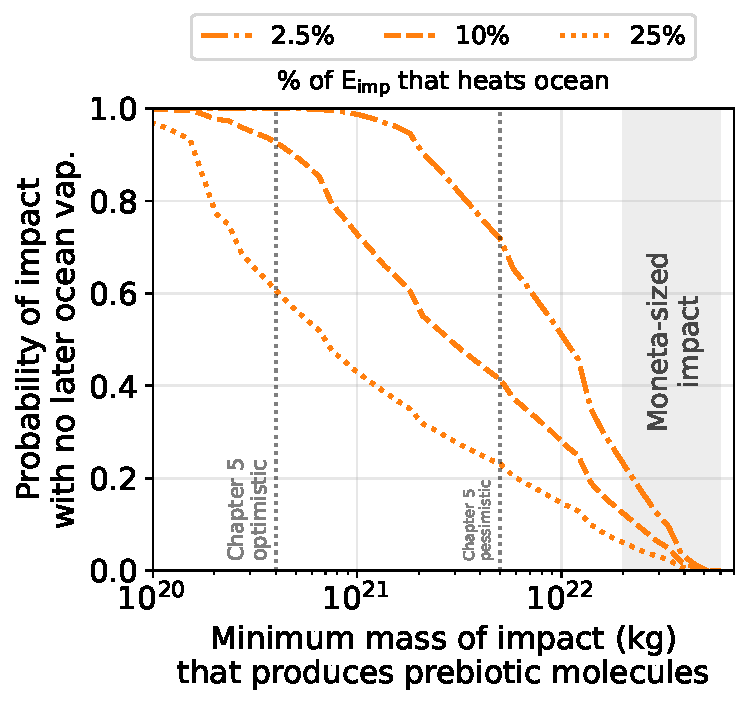
\includegraphics[width=0.55\textwidth]{tex/6time/figures_thesis/probabilities_of_impacts_sens.pdf}
  \caption{Similar to Figure \ref{fig:probabilities_of_impacts}, except we consider different values for the fraction of impactor energy that heats the ocean.}
  \label{fig:probabilities_of_impacts_sens}
\end{figure}

Figure \ref{fig:timing_sensitivity} shows the timing of the last impact to make conditions favorable for biopoiesis that does not experience subsequent ocean vaporization for $f_\mathrm{E,vap}$ values of 0.025, 0.1 (nominal value), and 0.25. As in the main text, we consider the Chapter \ref{ch:5} optimistic (Figure \ref{fig:timing_sensitivity}a) and pessimistic (Figure \ref{fig:timing_sensitivity}b) minimum impactor masses to produce significant prebiotic molecules. In Figure \ref{fig:timing_sensitivity}a, the timing of the last life-starting impact is relatively insensitive to $f_\mathrm{E,vap}$. In the Chapter \ref{ch:5} pessimistic case (Figure \ref{fig:timing_sensitivity}b), an origin of life is preferred later in the Hadean for larger values of $f_\mathrm{E,vap}$.

\begin{figure}
  \centering
  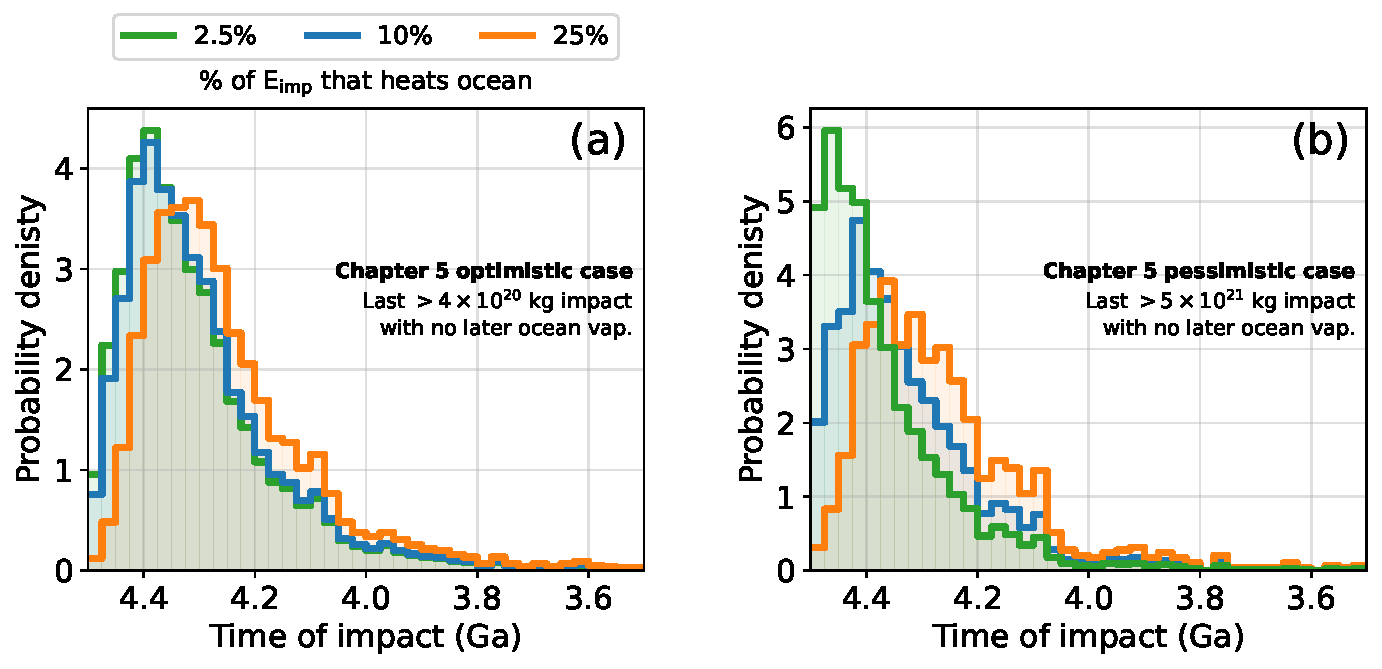
\includegraphics[width=1.0\textwidth]{tex/6time/figures_thesis/timing_sensitivity.pdf}
  \caption{Similar to Figure \ref{fig:time_and_mass}, except we consider different values for the fraction of impactor energy that heats the ocean.}
  \label{fig:timing_sensitivity}
\end{figure}

Overall, uncertainty in the impact properties required to vaporize the ocean has a small effect on our qualitative conclusions. Regardless of $f_\mathrm{E,vap}$, the origin of life on Earth from an impact does not appear to be a fluke (Figure \ref{fig:probabilities_of_impacts_sens}) and biopoiesis is preferred early in the Hadean with uncertainty spanning the entire eon (Figure \ref{fig:timing_sensitivity}). However, it is conceivable that a more complete understanding $f_\mathrm{E,vap}$ as a function of impact angle and other impact parameters could change these results.

\printendnotes

%
% ==========   Bibliography
%
\nocite{*}
\bibliographystyle{plainnat}
\bibliography{bib}
%
% ==========   Appendices
%
\appendix
\raggedbottom\sloppy
 
% ========== Appendix A
 
\chapter{the first appendix}
 

\end{document}